\documentclass{phd_class}%
\graphicspath{{images_hardlinked/}{images_simulation/}}%
\addbibresource{bibliography.bib}%

\begin{document}%
\pagecolor{gray!20}%
\tableofcontents%
\newpage%

\section{Random notes to sort}
\label{sec:random-notes-sort}

\begin{itemize}
\item When  in excited  state, qubit  emits a single  photon -  a Fock
  state, whose  phase is undefined.   Therefore this is  an incoherent
  emission.
\end{itemize}

\newpage

%% Fabrication
% -*- TeX-master: "../all_the_notes.tex" -*-

\section{Fabrication}
\label{sec:fabrication}

\textit{Fabrication is not  an easy thing, and yet it  can be completed
  in the space of a single week}

\subsection{No Category}
\label{sec:no-category}

\begin{framed}\noindent
  \begin{itemize}
  \item Always ground the qubits directly - never through a capacitor;
  \end{itemize}
\end{framed}

\subsection{Macroscopic parameters}\label{sec:size-parameters}
\begin{figure}[ht]
  \centering         \includegraphics[height=4cm]{fabrication_cassette}
  \includegraphics[height=4cm]{qubit_chip_annotated}
  \caption{\small   Big  markers   are   the   P,Q  markers   described
    below.\label{fig:qubit_chip}}
\end{figure}
\begin{enumerate}
\item \textbf{Sample chips} are mounted in a cassette with windows. The
  available sizes are:

  \begin{itemize}
  \item \iunit{18}{mm} x \iunit{18}{mm};
  \item \iunit{13}{mm} x \iunit{13}{mm};
  \item \iunit{8}{mm} x \iunit{8}{mm}.
  \end{itemize}

  \noindent \red{\textbf{The  chip must be  larger than this  window in
      order to be fixed in place.}}

\item \textbf{Qubit  chip}: \iunit{5}{mm} x \iunit{3}{mm}.   This means
  that a \iunit{18}{mm} chip will fit $ 3\times7 $ of them.

\item  \textbf{Transmission  line}:  is   characterized  by  width  and
  separation  with the  ground planes.   \red{\textbf{This defines  the
      impedance of the line, which must be 50$\Omega$}}.

  \begin{itemize}
  \item  \textbf{Narrow:}  Width  =  \iunit{20}{$\mu$m},  Separation  =
    \iunit{12}{$\mu$m};
  \item  \textbf{Wide:}   Width  =  \iunit{55}{$\mu$m},   Separation  =
    \iunit{30}{$\mu$m};
  \item  The  width  determines  the   speed  of  propagation  -  wider
    $ \equiv $ greater speed and higher frequencies.
  \end{itemize}

  \begin{center}
    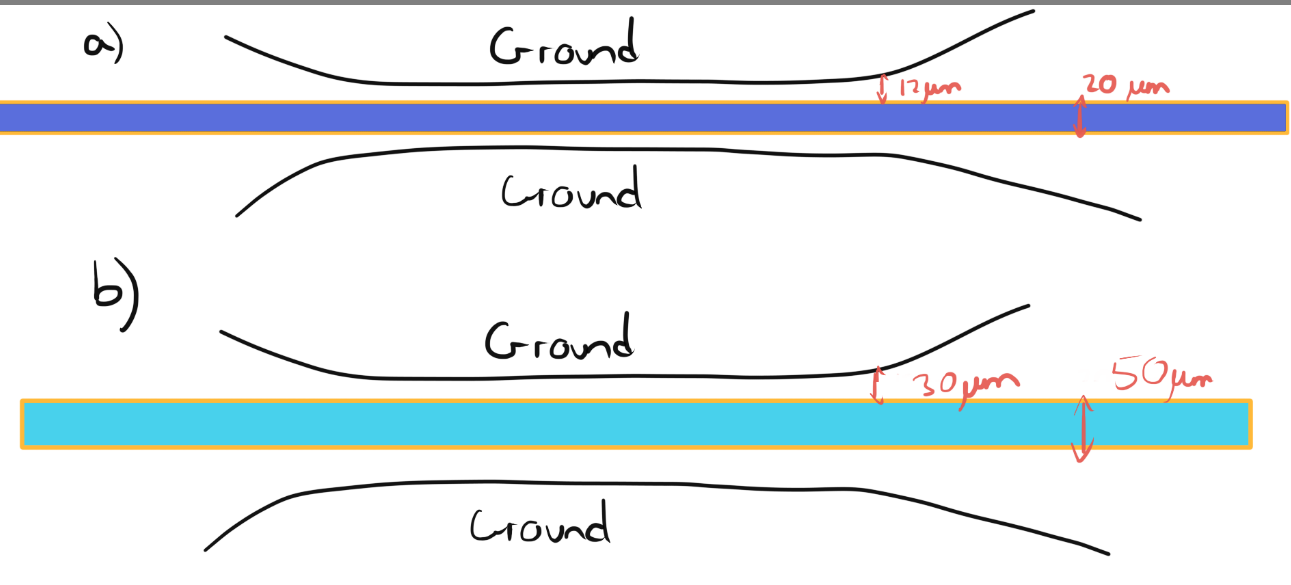
\includegraphics[height=3cm]{fab_transmission_line}
  \end{center}
\end{enumerate}

\subsection{Resonators}
\label{sec:resonators}

\noindent Resonators designed by Rais come in two lengths:
\begin{itemize}
\item \iunit{400}{$\mu$m};
\item \iunit{200}{$\mu$m}.
\end{itemize}

\noindent The frequency of a resonator is given by:

\begin{equation}
  \label{eq:fabrication_groupSpeed}
  \begin{aligned}
    & f j= \frac{v}{L_{r}}\\
    & \begin{cases}
      v = \frac{1}{\sqrt{L*C}}\\
      L = \text{ inductance per unit length}\\
      C = \text{ capacitance per unit length}\\
      L_{r} = \text{ length of resonator}
    \end{cases}
  \end{aligned}
\end{equation}

\noindent

\newpage\subsection{Materials parameters}
\label{sec:materials-parameters}

\begin{framed}\noindent
  In a charge qubit, the only  part that needs to be superconducting is
  the    JJ     superconducting-insulator-superconducting    structure.
  \red{\textbf{All other components  can be made from  normal metal, as
      there is no persistent current.}}
\end{framed}

\subsubsection{Transition temperatures}
\label{sec:trans-temp}
\begin{itemize}
\item NbN\hfill \iunit{4.5}{K};
\item Al \hfill \iunit{1.3}{K};
\item Ti \hfill \iunit{0.63}{K}.
\end{itemize}

\newpage\subsection{Deposition}
\label{sec:deposition}


\begin{itemize}
\item \textbf{Ground planes and  bonding contacts:} Ti (\iunit{10}{nm})
  - Au (\iunit{80}{nm})
\item \textbf{Aluminum JJ:}
  \begin{itemize}
  \item Copolymer 13\% \hfill \red{T = 600nm};
  \item  Either ZEP520a:Anisol  1:2  or ARP6200\  4\%  \hfill \red{t  =
      100nm};
  \item \red{\textbf{The undercut is 150\,nm}};
  \item Angle evaporation leads to:
    \begin{itemize}
    \item Shift in the pattern by $ T\tan(\alpha) $;
    \item Shortening of the pattern by $ t\tan(\alpha) $.
    \end{itemize}
  \item Meaning that  in order to get an overlap  between \red{red} and
    \gold{yellow} we need to shift the deposition holes;
  \end{itemize}
  \begin{figure}[h]
    \centering \includegraphics[height=8cm]{fabrication_angle}
    \caption{\small    Angle   $\alpha$    shifts   the    pattern   by
      $ T\tan(\alpha) $  and shortens it by $  t\tan(\alpha).$ Thus the
      pattern needs  to be made longer  and shifted to get  the desired
      structure. \label{fig:fabrication_angle}}
  \end{figure}
  \begin{itemize}
  \item Shift the bottom layer and top layer in opposite directions by
    \begin{equation}
      \label{eq:jj_overlap}
      \text{Shift} = T\tan(\alpha).
    \end{equation}
  \item  Elongate  the windows  \red{\textbf{on  the  inner sides}}  by
    \hfill \textbf{NO NEED TO DO THIS}
    \begin{equation}
      \label{eq:jj_elongate}
      \text{Elongate} = t\tan(\alpha),
    \end{equation}
  \end{itemize}
\end{itemize}
\begin{framed}\noindent
  For T  = \iunit{600}{nm} and  t = \iunit{100}{nm} and  12$^o$: \hfill
  \red{Shift = \iunit{150}{nm}};

  \noindent For T = \iunit{600}{nm}  and t = \iunit{100}{nm} and 9$^o$:
  \hfill \red{Shift = \iunit{110}{nm}};

  The separation between neighbouring holes for the resist to be stable
  is 100\,nm.



\begin{center}
  \red{After the first deposition the mask gets smaller, so avoid vertical symmetry} \\
\end{center}
\end{framed}

\subsubsection{Perpendicular deposition}
\label{sec:perp-depos}

A  better deposition  is  the  one that  was  proposed  by Rais,  where
deposition is done at 0 and 30 degrees.
\begin{figure}[h]
  \centering \inkfig{15cm}{0and30}
  \caption{\small  Perpendicular deposition  followed  by 30$^o$  angle
    deposition     will     remove     the    ``shadow''     of     the
    tbar.\label{fig:0and30}}
\end{figure}


\subsection{Coupling-capacitance}
\label{sec:coupling-capacitance}

\begin{framed}\noindent
  \begin{itemize}
  \item   Separation  of   elements   should  be   of   the  order   of
    \iunit{2}{$\mu$m};
  \item  \red{\textbf{Each  \iunit{10}{$\mu$m} of  parallel  structures
        adds on \iunit{1}{fF} of capacitance.}}
  \end{itemize}

   \begin{center}
     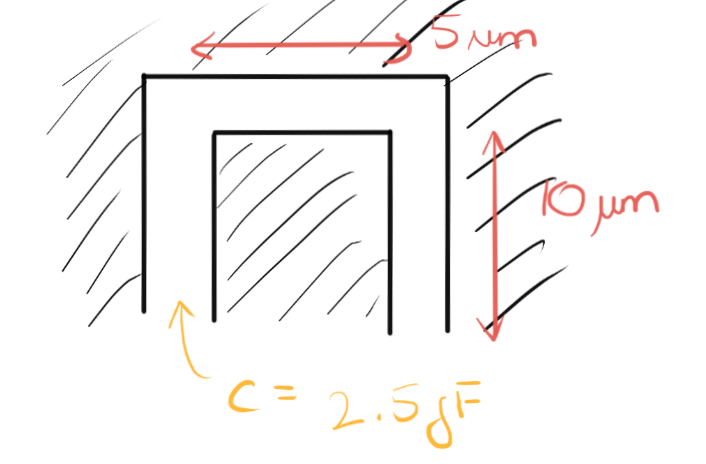
\includegraphics[height=4cm]{fab_capacitance} {\small  Think of it
       as counting the length of  the meander between structures.  Each
       \iunit{10}{$\mu$m}           of            length           adds
       \iunit{1}{pA}.\label{fig:example-image-c}}
   \end{center}
 \end{framed}


 \subsection{Josephson parameters}
 \label{sec:josephson-parameters}
 \begin{equation}
   \label{eq:fabrication_jj_1}
   \begin{aligned}
     & \red{E = E_J(1-\cos(\phi))} \\
     & \begin{cases}
       E_J = \frac{\Phi_0I_c}{2\pi}\\
       I_cR_n =  \frac{\pi\Delta(0)}{2e} \qquad  \text{critical current
         from BCS theory.}
     \end{cases}
   \end{aligned}
 \end{equation}

 \noindent A  typical JJ  will have  an area  of say  \iunit{100 \times
   200}{nm}$^{2}$

 \begin{framed}\noindent
   \begin{equation}\label{eq:fabrication_jj_2}
     \begin{aligned}
       & E_J = \frac{R_q}{R_n/N_{sq}}\frac{\Delta(0)}{2}\\
       & \begin{cases}
         R_n = 18.4\,\text{k}\Omega \qquad \text{sheet resistance of 100 } \times 100\,\text{nm}^{2}\\
         R_q = \frac{h}{(2e)^2}
       \end{cases}
     \end{aligned}
   \end{equation}
   \noindent The wider the JJ is in  squares, $ N_{sq} $, the lower the
   resistance   of  the   junction.   The   calibration  graph   for  a
   $ 200 \times \iunit{800}{nm}^2 $ junctions is shown below:

   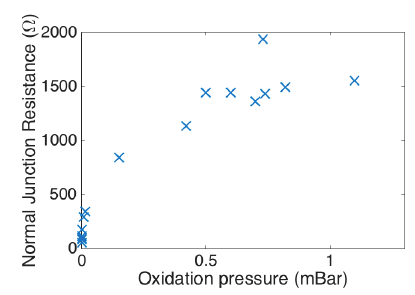
\includegraphics[height=4cm]{oxidation}

   \red{JJ resistance increases by $ \sim  10\% $ as one goes from room
     to cryogenic temperatures.}
 \end{framed}

 % The resistances go as follows:

 % \begin{table}[h]
 %   \centering
 %   \begin{tabular}{|c|c|c|}
 %     \textbf{Resistance}    & \textbf{Symmetrical JJ} & \textbf{Straddled}\\
 %     \iunit{1}{k$\Omega$} & 4838 & 2710 \\

 %   \end{tabular}
 %   \caption{Resistance of JJ}
 %   \label{tab:resistances_jj}
 % \end{table}


 \subsection{Capacitance parameters}
 \label{sec:capac-param}

\begin{equation}\label{eqn:sim_1}
  E_c = \frac{(2e)^2}{2C},
\end{equation}

\noindent  we need  the capacitance  of the  JJ. We  can treat  the two
overlapping parts of the JJ acting a parallel plate capacitor with

\begin{framed}\noindent
  \begin{equation}\label{key}
    C = \frac{\varepsilon\varepsilon_0A}{d},
  \end{equation}

  \noindent   with   the   permittivity  for   Aluminum   oxide   being
  $ \varepsilon \approx 10 $ and thickness $ d \approx \iunit{2}{nm} $.
  This  give s  a  junction 200  $ \times  $  800\,nm$^{2}$ a  charging
  frequency of $ E_c/\hbar \approx\iunit{19}{GHz} $.
\end{framed}

\newpage\subsection{Summary}
\label{sec:summary}

\hspace{-3cm}\begin{table}[h] \centering
  \begin{tabular}{|c|c|p{6cm}|c|}
    \hline\textbf{Energy} &  & \textbf{Variable  parameter} &
                                                              \textbf{Energy ($ N_{sq}=10, N_{NbN} = 5$)}\\\hline
    $ E_J $ & $ \frac{R_q}{R_{\square}/N_{sq}}\frac{\Delta(0)}{2} $ & $ R_q = \frac{h}{(2e)^2} = 6.484\,\text{k}\Omega,\newline \Delta = 1.73*(k_b\times 1.3\,\text{K}) = 3.1\times10^{-23}, \newline R_\square = \iunit{18.4}{k}\Omega $ & \iunit{77.5}{GHz}\\\hline

    $ E_C $ & $ \frac{(2e)^2}{2CN_{sq}} $ & $ \varepsilon = 10, d = \iunit{2}{nm}, \newline A = 100\times\iunit{100}{nm}^2, \newline C = \frac{\varepsilon\varepsilon_0A}{d} = \iunit{0.5}{fF} $ & \iunit{17.4}{GHz}\\\hline

    $       E_L       $       &        $       \frac{\Phi_0^2}{(2\pi)^22LN_{NbN}}       $       &
                                                                                                  $  \Phi_0 =  2\times10^{-15}\,\text{Wb}, \newline  L =
                                                                                                  \iunit{1.5}{nH}
                                                                                                  $
                                                                                                  per
                                                                                                  NbN
                                                                                                  square
                                                            &
                                                              \iunit{16.2}{GHz}\\\hline
  \end{tabular}
\end{table}


\newpage \subsection{Autocad-Beamer Design}
\label{sec:autocad-design}

\begin{itemize}
\item All shapes \textbf{must} be polylines.  They must be joined up in
  a single line, or they wont work;
\item Units are in microns;
\item \red{\textbf{Place small markers in the corners of the pattern so
      that centering is correct}};
\item Once design  is finished, \texttt{select all \ira  Purge \ira All
    \ira type "none*" \ira Yes to all};

\item \red{\textbf{Decide  on the  P, Q  markers that  will be  used to
      align the chip - note down their chip coordinates}}
\end{itemize}

\newpage\subsection{Typical exposure}
\label{sec:typic-expos-param}
\begin{itemize}
\item Depending  on the current you'd  like to use, you  have to choose
  between:
  \begin{itemize}
  \item High  Throughput: EOS  mode 3,  100 keV, lens  4, from  2nA and
    above
  \item High Resolution: EOS mode 6, 100 keV, lens 5, 100-400 pA.
  \end{itemize}
\item \iunit{100}{nA} for the bulky regions;
\item \textbf{Reading markers:}
  \begin{enumerate}
  \item Select window to work with: A, B, C or D;
  \item Find  global markers P,Q that  are usually on the  periphery of
    the chip (green)
  \item For each chip define a chip mark (blue) e.g. 490,490;
  \item Specify  the center the  central chip (-3500,2500) so  that the
    chip pattern is tied to the global markers.
  \end{enumerate}
  \begin{figure}[h]
    \centering \includegraphics[height=8cm]{jeol_layout}
    \caption{\small Red  is the  measured values of  the P,  Q markers.
      Green   is    the   designed   positions   that    are   set   as
      targets. \label{fig:jeol_layout}}
  \end{figure}
\end{itemize}
%
% -*- TeX-master: "all_the_notes.tex" -*-

\section{Experiment}

\subsection{S-parameters}
\label{sec:s-parameters}

\begin{equation}
  \begin{pmatrix}
    b_{1}\\b_2
  \end{pmatrix} = \begin{pmatrix} S_{11} & S_{12} \\ S_{21} & S_{22}
  \end{pmatrix}
  \begin{pmatrix}
    a_{1} \\ a_2
  \end{pmatrix}
\end{equation}

\begin{itemize}
\item $S_{11}$, is the input port voltage reflection coefficient;
\item $S_{12}$, is the reverse voltage gain;
\item $S_{21}$, is the forward voltage gain;
\item $S_{22}$, is the output port voltage reflection coefficient.
\end{itemize}

\begin{figure}[h]
  \centering \inkfig{5cm}{s_parameters}
  \caption{\small Measurement of tranmission and reflection\label{fig:s_parameters}}
\end{figure}
%

%% Quantum Electrodynamics
% -*- TeX-master: "../all_the_notes.tex" -*-
\newpage
\section{Dipole          operator          for          coupling          \cite{Astafiev2010}
  \cite{abdumalikov2010} \label{sec:dipole_coupling}}

\begin{framed}\noindent
  \textbf{Premise}

  We examine driving close to \iket{i}\ilra\iket{j}.
\end{framed}

\begin{minipage}[l]{0.5\linewidth}%
  %% Capacitive
  \begin{framed}\noindent
    \begin{equation}\label{eq:couple1}
      \begin{aligned}
        \hbar\Omega_{ij}\grey{\cos(\omega_{ij}t)} = \blue{\vartheta_{ij}}\iabs{V_\text{mw}}\grey{\cos(\omega_{ij}t)} & \\
        \blue{\vartheta_{ij} = C_\text{q-mw}V_\text{qubit}\zeta_{ij}} &
      \end{aligned}
    \end{equation}

    \begin{itemize}
    \item $ \iabs{V_\text{mw}} $:\hfill voltage amplitude in the transmission line;
    \item $ C_{q-mw} $:\hfill mutual capacitance between the line and qubit;
    \item $ V_\text{qubit} $:\hfill persitent voltage on the qubit;
    \item $ \zeta = \begin{pmatrix}
        \bra{0}\hat{A}\ket{0} & \bra{0}\hat{A}\ket{1} & \cdots\\
        \bra{1}\hat{A}\ket{0} & \bra{1}\hat{A}\ket{1} & \cdots\\
        \vdots & \vdots & \ddots
      \end{pmatrix} $:\hfill normalised (to unity) matrix elements.
    \end{itemize}%
  \end{framed}%
\end{minipage}%
\begin{minipage}[r]{0.5\textwidth}
  %% Inductive
  \begin{framed}\noindent

    \begin{equation}\label{eq:couple7}
      \begin{aligned}
        \hbar\Omega_{ij}\grey{\cos(\omega_{ij} t)} = \red{\vartheta_{ij}}\iabs{I_{mw}}\grey{\cos(\omega_{ij} t)}&  \\
        \red{\vartheta_{ij} = MI_p\zeta_{ij}} &
      \end{aligned}
    \end{equation}

    \begin{itemize}
    \item $ \iabs{I_{mw}} $:\hfill current amplitude in the transmission line;
    \item M:\hfill mutual inductance between the line and qubit;
    \item $ I_p $:\hfill persitent current in the loop;
    \item $ \zeta = \begin{pmatrix}
        \bra{0}\hat{A}\ket{0} & \bra{0}\hat{A}\ket{1} & \cdots\\
        \bra{1}\hat{A}\ket{0} & \bra{1}\hat{A}\ket{1} & \cdots\\
        \vdots & \vdots & \ddots
      \end{pmatrix} $:\hfill normalised (to unity) matrix elements.
    \end{itemize}

  \end{framed}
\end{minipage}
\begin{figure}[h]
  \centering 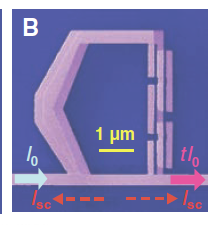
\includegraphics[height=4cm]{oleg_mutual}
\end{figure}

\noindent

\newpage

\begin{minipage}{0.5\linewidth}%
  %% Capacitive
  \begin{enumerate}%
  \item Writing out the charging energy in the  qubit, due to the qubits, $ Q_\text{qubit} $,
    and induced capacitively charges:

    \begin{equation}\label{eq:couple2} {\scriptsize
      \begin{aligned}
        E_C & = \frac{Q_\text{total}^2}{2C_\text{total}}\\
        & = \frac{1}{2C_\text{total}}\bigg[Q_\text{qubit} + {C_\text{q-r}V_{mw}}\bigg]^2\\
        & = {\frac{1}{2C_\text{total}}\bigg[Q_\text{qubit}^2 + \red{2Q_\text{qubit}C_\text{q-mw}V_\text{mw}} + C_\text{q-mw}^2V_\text{mw}^2\bigg]}\\
      \end{aligned}}
  \end{equation}
  \noindent Only the red terms are of interest for interaction, since they link the qubit and
  microwave systems.\red{Therefore only the red one is carried on}.

\item \begin{equation}\label{eq:couple3}
    \begin{aligned}
      E_c & = \frac{Q_\text{qubit}}{C_\text{total}}C_\text{q-mw}V_\text{mw}\\
      & = V_\text{qubit}C_\text{q-mw}V_\text{mw},
    \end{aligned}
  \end{equation}
  \noindent   where  we   have  the   residual  voltage   from  the   charge  on   the  qubit
  $ V_\text{qubit} $.

\item Now  let us take the  quantum mechanical operators  and evaluate with the  qubit states
  (which \textbf{do not} act on the microwave line operator $ \hat{V}_{mw} $):
  \begin{equation}\label{eq:couple4}
    \begin{aligned}
      \mathcal{H}_{int} & = \hat{V}_\text{qubit}\hat{C}_\text{q-r}\hat{V}_{mw} \\
      & = \sum_{i,j}\iketbra{i}{j}\blue{\bra{i}\hat{C}_{qr}\hat{V}_{\text{qubit}}\ket{j}} \hat{V}_{mw}\\
      & = \sum_{i,j}\iketbra{i}{j}\blue{\vartheta_{ij}} \hat{V}_{mw}\\
    \end{aligned}
  \end{equation}
\end{enumerate}
\end{minipage}%
\begin{minipage}{0.5\linewidth}%
  %% Inductive
  \begin{enumerate}%
  \item Writing out the  flux energy in the qubit, due to the  qubits, $ \Phi_\text{qubit} $,
    and induced, $ M_I $ magnetic fluxes:

    \begin{equation}\label{eq:couple8}{\scriptsize
      \begin{aligned}
        E_\Phi &= \frac{\Phi_\text{total}^2}{2L}\\
        & = \frac{1}{2L_{\text{total}}}\bigg[\Phi_\text{qubit} + MI_{mw}\bigg]^2\\
        &        =       \frac{1}{2L_\text{total}}\bigg[\Phi_\text{qubit}^2        +
        \red{2\Phi_\text{qubit}MI_{mw}} + M^2I_{mw}^2\bigg]
      \end{aligned}}
  \end{equation}
  \noindent Only the red terms are of interest for interaction, since they link the qubit and
  microwave systems.\red{Therefore only the red one is left}.

\item \begin{equation}\label{eq:couple9}
    \begin{aligned}
      E_\Phi &= \frac{\Phi_\text{qubit}}{L_\text{total}}MI_{mw}\\
      & = I_pMI_{mw}
    \end{aligned}
  \end{equation}

  \noindent where we added the persistent current in the loop $ I_p $.

\item Now  let us  take the  quantum mechanical  operators and  evaluare the  matrix elements
  \cite{Astafiev2010}:
  \begin{equation}\label{eqn:dipole_1}
    \begin{aligned}
      \mathcal{H}_{int} & = \hat{I}_{mw}\hat{M}\hat{I}_p\\
      & = \sum_{i,j}\iketbra{i}{j}\red{\bra{i}\hat{M}\hat{I}_p\ket{j}} \hat{I}_{mw}\\
      & = \sum_{i,j}\iketbra{i}{j}\red{\vartheta_{ij}} \hat{I}_{mw}\\
    \end{aligned}
  \end{equation}

\item \begin{equation}\label{eq:couple10} \red{\vartheta_{ij} = MI_p\zeta_{ij}}.
  \end{equation}

  \noindent  \red{Effectively  the  atom  transitions  from 1  persistent  current  state  to
    another.}

  Adding a  matrix element  factor, so  that only a  change of  state (\iket{0}\ilra\iket{1})
  generates a change

    \begin{equation}\label{eq:couple13}
      \iabs{MI_p}\zeta_{ij}.
    \end{equation}

  \end{enumerate}
\end{minipage}

\newpage

\begin{framed}
  \noindent Dispelling common myths: so what is the difference between

  \begin{equation}
    \label{eq:myth1}
    \delta A = \ibra{e}\hat{A}\iket{e} - \ibra{g}\hat{A}\iket{g} \qquad \text{and} \qquad \ibra{e}\hat{A}\iket{g}
  \end{equation}

  \noindent Well, it comes down to what elements you need from the interaction matrix:

  \begin{center}
    \includegraphics[height=4cm]{matrix_coupling}

    {\small These cross terms can be used in perturbation theory\label{fig:matrix_coupling}}
  \end{center}

\end{framed}
\begin{enumerate}

\item  $ \mathbf{\hat{V}_\text{qubit}}  $ is  the  qubit voltage  operator, which  next to  a
  transition reads

  \begin{equation}\label{eq:couple5}
    \hat{V}_\text{qubit} = \frac{2e}{C_\text{total}}\sigma_x.
  \end{equation}

\item $ \mathbf{\hat{V}_\text{mw}} $ is the microwave field operator
  \begin{equation}\label{eq:couple6}
    {\hat{V}_\text{mw} = \iabs{V_{\text{mw}}}\cos(\omega t)\bigg(a^\dagger +a\bigg)}
  \end{equation}
\item Fully we have

  \begin{equation}
    \begin{aligned}
      H_{int}&=2e\frac{\hat{C}_\text{q-mw}}{C_\text{total}}\iabs{V_{\text{mw}}}\cos(\omega t)\sigma_x\\
      &= \hbar\Omega\cos(\omega t)\sigma_x.
    \end{aligned}
  \end{equation}
\end{enumerate}

\begin{framed}\noindent
  \begin{equation}
    \mathcal{H}_{\text{int}}=g_0\big(\sigma^++\sigma^-\big)\big(a+a^\dagger\big),          \qquad
    g_0=V_{q0}C_{qr}V_{r0},
  \end{equation}
\end{framed}

\begin{enumerate}


\item  Now,  to express  the  value  $  \hat{I}_{mw}  = \iabs{I_{mw}}\cos(\omega_dt)$  as  an
  operator, we follow these reasons:
  \begin{itemize}
  \item The current which supplied the energy couples the
  \end{itemize}
  \noindent to get
  \begin{equation}\label{eq:couple15}
    \hat{I}_{mw} = \iabs{I_{mw}}\cos(\omega_{ij}t)\bigg(a + a\idagger\bigg).
  \end{equation}
\end{enumerate}

\begin{framed}\noindent
  So alltogether, the operator on the qubit system is
  \begin{equation}\label{eq:couple16}
    \begin{aligned}
      \mathcal{H}_{int} & = \sum_{i,j}{\bigg[\iabs{I_{mw}}\vartheta_{ij}\cos(\omega_{ij}t)\bigg]}\iketbra{i}{j}\\
      & = \sum_{i,j} \hbar\Omega_{ij} \cos(\omega_{ij}t) \iketbra{i}{j}\qquad \red{\hbar\Omega_{ij} = \iabs{I_{mw}}MI_p\zeta_{ij}}\\
    \end{aligned}
  \end{equation}

\end{framed}



\subsection{Summary \cite{Astafiev2010}}
\begin{framed}\noindent
  \noindent When a qubit system emits, the  strength of emission depends on the dipole moment
  of the system, as we saw in Chapter~\ref{sec:dipole_coupling}:
  \begin{equation}\label{eq:couple17}
    \vartheta_{ij} = \left[\begin{aligned}
        & \blue{C_{q-mw}V_\text{qubit}\zeta_{ij}} \qquad&& \text{\blue{capacitive coupling causes induced charge}}\\
        & \red{MI_p\zeta_{ij}} \qquad&& \text{\red{inductive coupling causes induced flux}}
      \end{aligned}\right.
  \end{equation}
\end{framed}

\noindent adding some  time dependence of $  \omega $, \textbf{since the system  will repospond at
  the rate of out driving}, and expanding out the matrix elements for a two level system

\begin{equation}\label{eq:couple18}
  \zeta = \begin{pmatrix}
    \bra{0}\hat{A}\ket{0} & \bra{0}\hat{A}\ket{1} \\
    \bra{1}\hat{A}\ket{0} & \bra{1}\hat{A}\ket{1} \\
  \end{pmatrix} \ira \begin{pmatrix} 0 & \red{\isigmaminus}\\\isigmaplus&0
  \end{pmatrix}
\end{equation}

\noindent we can concentrate on the \red{relaxation} matrix element to get

\begin{equation}\label{dipole_2level}
  \vartheta_{ij}(t) = MI_p\isigmaminus e^{-i\omega t}
\end{equation}

\newpage
%
\section{Emission from system} 
 Before we begin, let us clarify certain assumptions:
 \begin{itemize}
 	\item An atom left to itself in an excited state \textbf{will never decay};
 	\item Decay only occurs due to quantum noise. The most trivial case, is having two $ Z_0 $ resistors somewhere on the tranmission line:
 	
 	\ipic{3cm}{noise}
 	
 	\item  The quantum noise \textbf{\red{which is the variation of current squared}} is defined by
 	\begin{equation}\label{key}
 		S(w) = \red{\iaverage{j^2}} = \frac{1}{Z_0}\hbar\omega
 	\end{equation}
 	
 	\noindent but only a small part of it will be affecting relaxation of our $ \omega_0 $ qubit.
 	
 	\ipic{4cm}{noise_spectrum}
 	
	\item This mean square current, $ \iaverage{j^2} $ will interact with the flux being created by the switching state of the atom, $ \vartheta = MI_p\isigmaminus e^{-i\omega t} $, to give an energy
	
	\begin{equation}\label{key}
		E_\text{interaction}^2 = \iaverage{j^2}\vartheta^2 = \hbar\omega_0\frac{1}{Z_0}\vartheta^2
	\end{equation}
	
	\item The frequency associated with this energy (and hence the transition rate associated with this energy)
	
	\begin{equation}\label{key}
		\Gamma = \sqrt{\frac{E_\text{interaction}^2}{\hbar^2}} = \cdots (\text{ oleg promised to explain})
	\end{equation}
 \end{itemize} 

 \subsection{As derived in Oleg's papers \cite{abdumalikov2010}\cite{Astafiev2010}}
Here it is written, that relaxation occur due to quantum noise in the system:
\begin{equation}\label{key}
\Gamma_{ij} = \hbar\omega_{ij}\frac{\vartheta_{ij}^2}{\hbar^2Z_0},
\end{equation}

\noindent which depends on
\begin{itemize}
	\item The energy associated with the transition\hfill $ \hbar\omega_{ij} $;
	\item The dipole matrix transition element \hfill $ \vartheta_{ij} = \bra{i}U\ket{j} \equiv MI_\text{PC}\zeta_{ij}$;
	\item The impedance of the line \hfill $ Z_0 $;
\end{itemize}

\subsection{Atom emission}
The atom will scatter waves according to
\[
I_\text{sc}(x,t) = \big[i\frac{\hbar\Gamma_{21}}{\phi_{21}}\iaverage{\sigma_{21}}\big]e^{ik\iabs{x}-\omega_{21}t},
\]

\noindent and \iaverage{\sigma_{21}} is found from the stationary state of the Master equation $ \dot{\rho} = 0 $. The transmission coefficient is:

\[
\begin{aligned}
t = & \frac{\text{Input current + scattered current}}{\text{Input current}} \ge 1\\
& = 1 + \big[i\frac{\hbar\Gamma_{21}}{\phi_{21}}\iaverage{\sigma_{21}}\big]\red{e^{ik\iabs{x}-\omega_{21}t}}/\frac{\hbar\Omega_{21}}{\phi_{21}}\quad \red{\text{ignore}}\\
& = 1 + i\frac{\Gamma_{21}}{\Omega_{21}}\iaverage{\sigma_{21}}
\end{aligned}
\]

\iframe{The relaxation rate is caused by quantum noise in the 1D space:
	\[
	\Gamma_{21} = \hbar\omega_{21}\bigg(\frac{MI_\text{persistent}}{\hbar}\bigg)^2\frac{1}{Z}
	\] 
}

\subsection{Emission by the atom\label{subsec:Scattering}}  
\iframe{The input-output theory shows that the average field emitted by an artificial atom to an open transmission line is

\begin{equation}\label{theoEmission}
\iexpectation{V_{\text{sc}}} =  i\sqrt{\frac{\Gamma_{ij}}{2}}\iexpectation{\sigma_{ji}},
\end{equation}}

\noindent where $ \iexpectation{\sigma_{ji}}=\text{Tr}\left\lbrace \ketbra{j}{i}\rho \right\rbrace = \rho_{ij} $, and $ \Gamma_{ij} $ is the \iket{i}\lra\iket{j} relaxation rate. The angular frequency of the emission is $ \omega_{ij} $.
\begin{itemize}
	\item $ V_{\text{L}}^{+} $ resonant input with the \iket{i}\lra\iket{j} transition and defined by Eq.~\eqref{theoField};
	\item $ V_{\text{L}}^{-} = V_{\text{L}}^{+}+V_{\text{sc}}$ the transmitted field, which is a combination of the incident and emitted fields\footnote{The artificial atom, whose dynamics, Eq.~\eqref{rwaHamitlonianApprox}, are determined by the incident field, is treated as a stand-alone quantum system that emits a field $ V_{\text{sc}} $. This resultant field is a sum of the incident, $V_{L}^{+} $, and emitted, $ V_{\text{sc}} $, fields, created by two distinct objects in the quantum system.};
	\item $ V_{\text{R}}^{-} = - V_{\text{sc}}$ the reflected field, only composed of emission by the artificial atom.
\end{itemize}

The transmission, $ t $, and reflection, $ r $, coefficients are defined as

\begin{equation}\label{theoRefTran}
\begin{aligned}
t & = \frac{\iexpectation{V_{\text{L}}^{-}}}{\iexpectation{V_{\text{L}}^{+}}} = 1+\frac{i\Gamma_{ij}}{\iexpectation{V_{\text{L}}^{+}}\sqrt{2\Gamma_{ij}}}\rho_{ij};\\
r & = \frac{\iexpectation{V_{\text{L}}^{-}}}{\iexpectation{V_{\text{L}}^{+}}} = 1-t;
\end{aligned}
\end{equation}

\noindent where $\iexpectation{V} = \frac{1}{T}\int_{0}^{T}V(t)dt$ is the average voltage over a normalisation time $ T $. Since the Rabi frequency, $ \Omega $, is related to the drive amplitude, $ \iexpectation{V_{\text{L}}^{+}}  $,

\begin{equation}
\Omega_{ij}=\iexpectation{V_{\text{L}}^{+}}\sqrt{2\Gamma_{ij}},
\end{equation}

\noindent Equation~\eqref{theoEmission}, \eqref{theoRefTran}, reduce to

\begin{equation}\label{theoCoeff}
\begin{aligned}
t & = 1 + i\frac{\Gamma_{ij}}{\Omega_{ij}}\rho_{ij};\\
r & = 1-t.
\end{aligned}
\end{equation}

\noindent The coefficients of Eq.~\eqref{theoCoeff} apply to coherent emission, when angular frequencies of the driving and emitted fields coincide, $ \omega^{d}_{ij} \approxeq\omega_{ij} $, and interference between the onset and emitted waves occur.  	

  \subsection{Single drive configuration\label{subsec:singleDrive}}
When a single drive couples two levels \iket{i}, \iket{j}, the non-interacting third level can be traced out from Eq.~\eqref{rawTransformedFinal}-\eqref{linLinTerm}. The procedure of solving the Master equation, and determining~$ \rho $, was done with \texttt{Mathematica}. The $ \rho_{21} $, $ \rho_{31} $ coefficients obtained, for respective \iket{1}\lra\iket{2}, \iket{1}\lra\iket{3}, drives, upon substitution into Eq.~\eqref{theoCoeff} give

\begin{equation}
r_{21}=\frac{\Gamma_{21}}{2\gamma_{21}}\frac{1+i\delta\omega_{21}/\gamma_{21}}{1+(\delta\omega_{21}/\gamma_{21})^2+\Omega_{21}^2/\Gamma_{21}\gamma_{21}}; \quad r_{31}=\frac{\Gamma_{31}}{2\gamma_{31}}\frac{1+i\delta\omega_{31}/\gamma_{31}}{1+(\delta\omega_{31}/\gamma_{31})^2+\Omega_{31}^2/\Gamma_{31}\gamma_{31}},
\label{singleReflectance}
\end{equation}

Figure~\ref{singleDriveReflection} shows the real components of $ r_{ij} $ as function of the detuning of the driving field from the atomic transition, $ \delta\omega_{ij} = \delta\omega_{ij}^{d}-\delta\omega_{ij}$. The reflectance peak corresponds to the case when the atom relaxes to the ground state, and emits a photons that is coherent~\footnote{Of the same frequency.} with the incident field, but shifted by a phase of $ \pi $.\footnote{Signified by the $ i $ factor in Eq.~\eqref{theoCoeff}.} Destructive interference occurs with the incident field and the wave is fully reflected.

\begin{figure}[h]
	\ipic{5cm}{transmission_purely_theoretical}
	\caption{\small \textbf{Simulations of elastic scattering of an incident microwave in an arbitrary $ \mathbf{\ket{i}, \ket{j}}, $ system}. Shown are the real part of the reflection coefficient, $ \re{r_{ij}} $, evaluated with Eq.~\eqref{singleReflectance} for $ \Gamma_{ij}=50, \Gamma_{\phi,ij}=5 $, for a range of driving powers, $ \Omega_{ij} $. When the incident field is on resonance with the atomic transition, $ \delta\omega_{ij}=0  $, the reflectance curve exhibits a peak, as emission from the artificial atom undergo destructive interference with the incident wave. The weaker the driving power, the stronger this interference becomes.}
	\label{singleDriveReflection}
\end{figure}

The sharpness of the central features diminishes for larger driving amplitudes, $ \Omega $. As the number of photons in the transmission line grows, the photon emitted by the atom cannot interfere with all the ones propagating down the transmission line. This photon overload causes $ t $ and $ r $ to become insensitive to atomic transitions.  To saturate the peak, one applies weak drives, $ \Omega_{ij}<<\Gamma_{ij}\gamma_{ij} $ in which case Eq.~\eqref{singleReflectance} no longer depends on the driving amplitude

\begin{equation}
\begin{aligned}
\re{r_{21}} = \frac{\Gamma_{21}}{2\gamma_{21}}\frac{1}{1+(\delta\omega_{21}/\gamma_{21})^2}; \quad \re{r_{31}}=\frac{\Gamma_{31}}{2\gamma_{31}}\frac{1}{1+(\delta\omega_{31}/\gamma_{31})^2},
\end{aligned}
\label{singleLorentzian}
\end{equation}

\noindent allowing on to determine the decoherence rates  $ \gamma_{ij}, \Gamma_{ij} $ from fittings to observed values.


\subsection{Combining the sections above}
 Emission from a system is linked to the voltage operator, $ V^{+} $.
 \begin{itemize}
 	\item The voltage operator is defined as:
 	
 	\begin{equation}\label{feb22018}
 	\hat{V}^{+} = i\frac{\hbar\Gamma_1}{\phi}\sigma^{-},
 	\end{equation}
 	
 	\noindent the `-' coming from the fact that the atom must relax in order for voltage to be produced. The average produced field would be
 	
 	\[
 	\iaverage{\hat{V}^{+}} = i\frac{\hbar\Gamma_1}{\phi}\iaverage{\sigma^{-}},
 	\]
 	
 	\item Now, the power resulting from this voltage, which is effectively noise as the atom relaxes spontaneously, can be found:
 	
 	\begin{equation}\label{feb22018:1}
 	\begin{aligned}
 	\iaverage{V^2(\omega)} = & \frac{1}{2\pi}\int_{-\infty}^{\infty}\iaverage{\hat{V}^{-}(0)\hat{V}^{+}(\tau)}e^{i\omega \tau}d\tau\\
 	= & \frac{\hbar^2\Gamma_1^{2}}{\phi^2}\frac{1}{2\pi}\int_{-\infty}^{\infty}\iaverage{\sigma_{+}(0)\sigma_{-}(\tau)}e^{i\omega \tau}d\tau
 	\end{aligned}
 	\end{equation}
 	
 	\item \red{Using a trick in Olegs book, one can find that the term $ \iaverage{\sigma_{+}(0)\sigma_{-}(\tau)} $ can be decomposed as:
 		\begin{itemize}
 			\item \textbf{Total sum is} \[ \frac{1+{\isigmaz}}{2}. \]
 			\item \textbf{The coherent part is} \[ \iaverage{\sigma_{+}}\iaverage{\sigma_{-}}. \]
 			\item \textbf{Therefore the incoherent part must be the difference between the two}: \[ \frac{1+{\isigmaz}}{2} - \iaverage{\sigma_{+}}\iaverage{\sigma_{-}}. \]
 		\end{itemize}
 	} 
 	
 	\item Finding the total emitted power, by integrating over the full frequency range \red{and assuming that we are dealing with stationary states (ss) that would form in the system when averaging:}
 	
 	\begin{equation}\label{feb220183}
 	\begin{aligned}
 	\text{Power}_\text{total} &= \frac{1}{Z}\int 	\iaverage{V^2(\omega)}  d\phi\\
 	& = \frac{1}{Z}\int \frac{\hbar^2\Gamma_1^{2}}{\phi^2}\frac{1}{2\pi}\int_{-\infty}^{\infty} \frac{1+{\isigmaz}_{ss}}{2} e^{i\omega \tau}d\tau   d\phi\\
 	& = \frac{\hbar^2\Gamma_1^2}{Z\phi^2} \frac{1+{\isigmaz}_{ss}}{2} \int\frac{1}{2\pi}\int e^{i\omega\tau}d\tau d\phi\\
 	& \text{Using the fact that the integral over the delta function is just 0 and } \Gamma_1 = \frac{\hbar\omega\phi^2Z}{\hbar^2}\\
 	& = \hbar\omega\Gamma_1  \frac{1+{\isigmaz}_{ss}}{2}
 	\end{aligned}
 	\end{equation}
 	
 	\noindent Now, because we are driving continously, decoherence will result in our rotation of the state from \iket{0} to \iket{1} to form an intermediate value when $ \isigmaz = 0 $ and so the maximum emitted power from the atom will be:
 	
 	\iframe{\begin{equation}\label{key}
 		\text{Power}_\text{total} = \frac{\hbar\omega\Gamma_1}{2}	
 		\end{equation}}
 	
 	
 	\item Now, redoing the same, but only considering the coherent contribution i.e. instead of $  \frac{1+{\isigmaz}_{ss}}{2} $ use $ \iaverage{\sigma_{+}}\iaverage{\sigma_{-}} $ we round up at:
 	
 	\begin{equation}\label{maximalCoherentEmission}
 	\begin{aligned}
 	\text{Power}_\text{coherent} &= \hbar\omega\Gamma_1 \iaverage{\sigma_{+}}_{ss} \iaverage{\sigma_{-}}_{ss} = \text{ upon subbing in the obtained expectationv values }\\
 	& = \hbar\omega\Gamma_1\bigg(\frac{2\Gamma_1\Omega}{2\Gamma_1^2+\Omega^2}\bigg)\\&\Rightarrow \text{max value } = \frac{\hbar\omega\Gamma_1}{8}
 	\end{aligned}
 	\end{equation}
 	
 	\begin{itemize}
 		\item \red{You can measure this power with the SPA i.e. you measure 1/8 of a single photon power;}
 		\item Then, you can tune your VNA power to match this $ 8\times $ coherent signal power, and be supplying exactly one photon to the system. Then there will be no leakages, as the photon will be absorbed by the system, with no leftover for leaking;
 	\end{itemize}
 	\item The total number of photons in the system can be found from 
 	\begin{equation}\label{key}
 	N = \frac{\Omega}{\Gamma_1}
 	\end{equation}
 \end{itemize} 
 
 \newpage
 
\subsection{Coherent and incoherent emission}
 \begin{enumerate}
 	\item \textbf{Coherent field}, means a fixed phase relation with the two input fields. For example, supplying $ e^{i\omega_1t} $ and $ e^{i\omega_2t} \iright e^{i(\omega_1+\omega_2)t + \phi}$ where $ \phi $ is a fixed value. This allow further entanglement procedures;
 		\item \textbf{Emission by qubit} can be characterised as coherent and incoherent emission. One needs to work with \iaverage{\sigma_i} values and look at the corresponding bloch sphere. 
 	
 	\begin{figure}[h]
 		\ifigure{7cm}{sphere}
 	\end{figure}
 	
 	Recalling that
 	
 	\red{{\large \begin{equation}\label{expectationPauli}
 			\rho_{00} = \frac{\iaverage{\sigma_z}+1}{2};\quad \rho_{01}=\frac{\iaverage{\sigma_x}-i\iaverage{\sigma_y}}{2} = \iaverage{\sigma_{+}};\quad\rho_{10}=\frac{\iaverage{\sigma_x}+i\iaverage{\sigma_y}}{2} = \iaverage{\sigma_{-}};
 			\end{equation}
 			\begin{equation}\label{expectationPauli2}
 			\iaverage{\sigma_x}=\rho_{01}+\rho_{10};\quad\iaverage{\sigma_y} = i\rho_{01}-i\rho_{10};\quad\iaverage{\sigma_z}=\rho_{00}-\rho_{11}
 			\end{equation}}}
 	
 	\noindent The more a state is on the equator, the more coherence it has since a superposition is formed. Recall that, so that when the ``arrrow'' projects fully onto the equator, it means that the atom is in a superposed state e.g. $ \frac{\iket{0}+\iket{1}}{\sqrt{2}} \ra \imatrix{1/2}{1/2}{1/2}{1/2} \ra \isigma_z = 0, \isigma_x = 1$ (or some other rotation around y).
 	
 	\begin{center}
 		\textbf{Coherent emissions $ \propto \isigmax$\newline
 			Incoherent $ \propto\isigmaz $. \large}
 	\end{center}
 	\red{Both emissions will occur at the frequency of the qubit $ \omega_0 $ (i.e. energy level separaion), but emission from \isigmax will be sharp, while incoherent emission from \isigmaz will be broad as shown below}
 	
 	\ipic{5cm}{emission}
 	\item Now draw the parrallels between:
 	
 	\begin{itemize}
 		\item The field in a resonator \hfill \ia\ and \iadagger;
 		\item Qubit\hfill excitation $ \sigma_{+} = \ketbra{1}{0} = \imatrix{0}{0}{1}{0} = (\sigma_x-i\sigma_y)/2$ and relaxation $ \sigma_{-} = \ketbra{0}{1} = \imatrix{0}{1}{0}{0} = (\sigma_x+i\sigma_y)/2$
 		
 	\end{itemize}
 	in the following way
 	
 	\begin{center}
 		\begin{tabular}{|c|c|c|}
 			\hline 
 			\textbf{Coherent field} & $ \big(\ia + \iadagger\big) $ & $ \isigmax $ \\ 
 			\hline 
 			\textbf{Photon number} & $ \ia\iadagger $& \isigmaz \\ 
 			\hline 
 		\end{tabular} 
 	\end{center}

\end{enumerate}
\newpage %
\section{Scattering by system \cite{Astafiev2010}}
 \iframe{
 	\begin{equation}\label{key}
 				2ikV_{sc} = i\omega \phi_p\iaverage{\sigma_{-}}.
 	\end{equation}
	}
	Now we consider a system scattering waves due changing it's state:
	
	\ipic{5cm}{scattering}
	
 \begin{enumerate}
 	\item Beggining with the telegraph equations for the voltage difference at the position of the atom:
 	\begin{equation}\label{7thFeb1}
 	\left\lbrace\begin{aligned}
 	\difffrac{\Delta V}{x} & = l\difffrac{I}{t}\\
 	\Delta V & = \iabs{V_{sc}}\left[e^{i(kx - \omega t)} - e^{i(-kx - \omega t)}\right]
 	\end{aligned}\right. \Rightarrow \difffrac{\Delta V}{x} = 2ikV_{sc}
 	\end{equation}
 	
 	\item Now, the atom is situated specific point on the line, $ x = 0 $, \red{\textbf{and only at this point is the voltage discontinous.}} Thus we incoporate delta function into Eq.~\eqref{7thFeb1}
 	\begin{equation}\label{7thFeb4}
 	\frac{d\Delta V}{dx} = 2ikV_{sc}\delta(x)
 	\end{equation}
 	
 	\item This voltage is caused by a change of the linked flux (dipole) during a transition (Eq.~\eqref{dipole_2level})
 	
 	\begin{equation}\label{key}
 		\text{small change in flux } = \vartheta_{ij}(t) = MI_p\isigmaminus e^{i\omega t}.
 	\end{equation}
 	
 	\item Let's evaluated the induced voltage due to this changing of flux
 	
 	\begin{equation}\label{7thFeb5}
 		\Delta V = \dot{\Phi} = i\omega MI_p\isigmaminus e^{i\omega t}
 	\end{equation}
 	
 	\item Integrating Eq.~\eqref{7thFeb4} and subbing in Eq.~\eqref{7thFeb5} we arrive at
 	
 	\begin{equation}\label{7thFev5}
 	2ikV_{sc} = i\omega\phi_p\iaverage{\sigma_{-}}\qquad \phi_p = MI_pe^{i\omega t}
 	\end{equation}
 	
 \end{enumerate}%
\section{Relaxation due to noise}
% A system coupled to resonators in thermal equilibrium energy exchange
% depends   on    the   temperature   of   these    resonators.    When
% $ kT>>\hbar\omega $ photons will  be exchanged between the medium and
% system. When $ kT<<\hbar\omega $  the system will remain indefinitely
% in the ground state
\subsection{Relaxation from the noise spectrum}

\begin{figure}[h]
  \centering 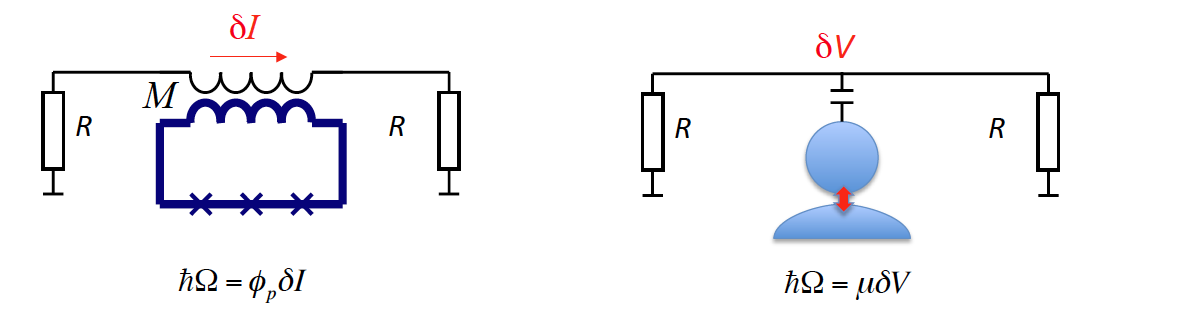
\includegraphics[height=4cm]{noise1}
\end{figure}

\noindent

\noindent In the  systems above noise may come from  current or voltage
fluctuations. We  shall analyse the  latter case, in which  the voltage
fluctuation acts as an effective driving field

\begin{equation}\label{noise1}
  \mathcal{H} = -\frac{\hbar\omega}{2}\sigma_z+\frac{\mu\delta V(\omega)}{2}\sigma_x\cos(\omega t);\quad\delta V(\omega) = \frac{1}{T}\int_{-T/2}^{T/2}\delta V(t e^{-i\omega t})dt,
\end{equation}

\noindent and after applying the RWA

\begin{equation}\label{noise2}
  \mathcal{H} = \frac{\mu\delta V(\omega)}{2}\sigma_x,
\end{equation}

\noindent the evolution of a system state

\begin{equation}\label{noise3}
  U(T)\iket{0} = \iket{0} - \frac{\mu\delta V(\omega)}{2}\frac{T}{\hbar}\iket{1} \quad \rightarrow \quad P_1 = \frac{\mu^2T^2}{4\hbar^2}\iaverage{\delta V^2},
\end{equation}

\noindent and incorporating  the spectral noise density $  S(\Omega) $ which
we integrate  over in  the frequency  range $  \Delta\omega =  2\pi/T $
(longer  acquisition time  means narrower  spectrum of  noise since  we
average more  and more, and only  low frequency remains will  remain in
the system.)

\begin{equation}\label{noise4}
  \begin{aligned}
    \iaverage{\delta V^2}&=S(\omega)\frac{2\pi}{T}\\
    P_1 &= \frac{\mu^2T^2}{4\hbar^2}\iaverage{\delta V^2}
  \end{aligned}\Rightarrow P_1 = \frac{\pi\mu^2}{2\hbar^2}S(\omega)T \rightarrow \text{ rate of
    excitation } \approx \Gamma = \frac{\pi\mu^2}{2\hbar^2}S(\omega).
\end{equation}


\begin{figure}[h]
  \centering 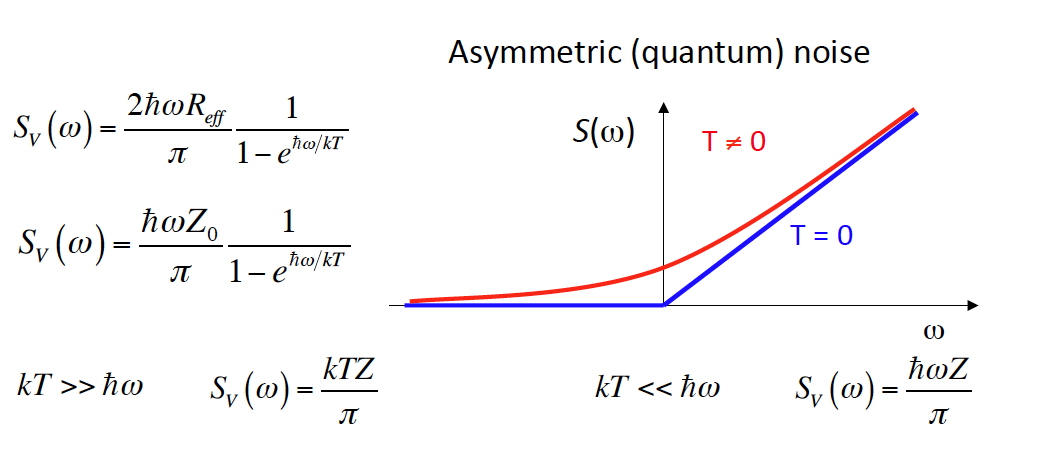
\includegraphics[height=4cm]{noise2}
\end{figure}

\newpage
%
\section{Unitary       transformations       and      the       rotating
  frame\label{sec:unitary}}
The Hermitian conjugate of an operator is defined as

 \begin{equation}\label{uniHermetian}
   U^{\dagger} = (U^{*})^{T},
 \end{equation}

 \noindent and the operator can be classified under two types

 \begin{itemize}
 \item $ U^{\dagger}\equiv U $ a Hermitian operator;
 \item $ U^{\dagger}\equiv U^{-1} $ is a unitary operator.
 \end{itemize}

 The most important equation for unitary operators is

 \begin{equation}\label{uniDef}
   U^{\dagger}U=\mathbb{I},
 \end{equation}

 \noindent    examples    of    which   are    Pauli    spin    matrices
 $ \sigma_x, \sigma_y, \sigma_z $.
 \begin{framed}
   \red{Now we  shall examine {the  rotation operator}, {  which rotates
       the state of  a two levels system  by an angle $  2\alpha $ about
       the $ j $ axis of the Bloch sphere}}
 \end{framed}

 \red{\begin{equation}
     \begin{aligned}
       U &= \exp\bigg[i\alpha\sigma_j\bigg] = \sum_{k}\frac{(i\alpha)^k}{k!}\sigma_j^k \\&= \sum_{k=0}\frac{{\alpha^{2k}(-1)^k}}{2k}\mathbb{I}+i\sum_{k=0}\frac{{\alpha^{2k+1}(-1)^k}}{2k+1}\sigma_j\\
       &= \cos(\alpha)\mathbb{I}+i\sin(\alpha)\sigma_j,
     \end{aligned}
   \end{equation}}

 \noindent where we  utilise $ \sigma_j\sigma_j = \mathbb{I}  $. For the
 three Pauli spin matrices this will read

 \begin{equation}\label{uniPauli}
   U(\sigma_x) = \begin{pmatrix}
     \cos{\alpha} & i\sin{\alpha}\\i\sin{\alpha}&\cos{\alpha}
   \end{pmatrix};\quad   U(\sigma_u)   =   \begin{pmatrix}   \cos{\alpha}   &
     \sin{\alpha}\\-\sin{\alpha}&\cos{\alpha}
   \end{pmatrix};\quad  U(\sigma_z)  =   \begin{pmatrix}  e^{i\alpha}  &
     0\\0&e^{-i\alpha}
   \end{pmatrix}.
 \end{equation}

 \noindent  Furthermore,  one can  double  check  the unitarity  of  the
 matrix:

 \begin{equation}\label{uniunitary}
   U^{\dagger}U =\bigg( \cos(\alpha)\mathbb{I}+i\sin(\alpha)\sigma_j\bigg)bigg( \cos(\alpha)\mathbb{I}-i\sin(\alpha)\sigma_j\bigg) = \mathbb{I}\cos^2(\alpha)+\sigma_j\sigma_j\sin^2(\alpha)\equiv\mathbb{I}.
 \end{equation}

 \noindent         When         a         unitary         transformation
 \red{$  \Psi'=U\Psi \leftrightarrow  \Psi =  U^{\dagger}\Psi'$} is  applied, the  \schrodinger
 equation will be modified as such

 \begin{equation}\label{duninewschroer}
   \begin{aligned}
     i\hbar\frac{dU^{\dagger}\Psi'}{dt} & = \mathcal{H}U^{\dagger}\Psi'\\
     i\hbar{U}^{\dagger}\frac{d\Psi'}{dt} + i\hbar\dot{U}^{\dagger}{\Psi'} & = \mathcal{H}U^{\dagger}\Psi' \quad\text{ \red{no time dependance of $ U $}}\\
     i\hbar\frac{d\Psi'}{dt} & = \bigg[U\mathcal{H}U^{\dagger} \red{-i\hbar U\dot{U}^{\dagger}}\bigg]\Psi'\\
   \end{aligned}
 \end{equation}

\begin{framed}\noindent
  Expectation values are conserved in unitary transformations:
  \[
    \begin{aligned}
      \bra{\psi}A\ket{\psi} & \equiv \left(\bra{\psi}U\right)U\idagger AU\left(U\idagger\ket{\psi}\right)\\
      & \equiv \bra{\psi'}A'\ket{\psi'}
    \end{aligned}
  \]
  \red{So   expectation  values   of  an   operator  remain   unchanged.
    \textbf{This  means that  physical  quantities can  be equally  well
      calculated in transformed frames e.g.  enter the rotating frame to
      find \isigmax.}}
\end{framed}

\noindent Also  important are  commutation properties between  the three
Pauli Matrices

 \begin{equation}\label{uniComm}
   \sigma_i\sigma_j=-\sigma_j\sigma_i,
 \end{equation}

 \noindent  which  results  in  the following  relations  involving  the
 unitary operator of rotation about the y-axis

 \begin{equation}\label{uniComm1}
   \left\lbrace\begin{aligned}
       U_{y}\sigma_z & = \bigg(\cos(\alpha)\mathbb{I}+i\sin(\alpha)\sigma_y\bigg)\sigma_z = \sigma_z\bigg(\cos(\alpha)\mathbb{I}-i\sin(\alpha)\sigma_y\bigg) = \sigma_zU_y^{\dagger}\\
       U_{y}\sigma_x & = \sigma_xU_y^{\dagger}\\
       U_{y}\sigma_y & = \sigma_yU_y\\
     \end{aligned}\right.
 \end{equation}

 \subsection{Example application\label{subsec:ExampleApplication}}
 A general  two levels system with  energy separation $ \varepsilon  $ interaction
 between the two states of strength $ \Delta $ can be written

 \begin{equation}
   \label{l1-uni}
   \begin{aligned}
     \mathcal{H} = \left(\begin{matrix} -\epsilon/2 & 0\\ 0 & \epsilon/2
       \end{matrix}\right) + \begin{pmatrix}
       0 & -\Delta/2\\-\Delta/2 & 0
     \end{pmatrix} & = {-\frac{\epsilon}{2}\sigma_z-\frac{\Delta}{2}\sigma_x}\\
     & = -\frac{\sqrt{\epsilon^2+\Delta^2}}{2}\left(\frac{\epsilon}{\sqrt{\epsilon^2+\Delta^2}}\sigma_z+\frac{\Delta}{\sqrt{\epsilon^2+\Delta^2}}\sigma_x\right)\\
     & = -\frac{\Delta E}{2}\left(\cos\left(\theta\right)\sigma_z+\sin\left(\theta\right)\sigma_x\right)\\
     {\Rightarrow \left\lbrace\begin{aligned}
           \mathcal{H} & = -\frac{\Delta E}{2}\big(\sigma_z\cos(\theta)+\sigma_x\sin(\theta)\big)\\
           \Delta E & = \sqrt{\epsilon^2+\Delta^2}\\
           \tan(\theta) & = \frac{\Delta}{\epsilon}
         \end{aligned}\right.}
   \end{aligned},
 \end{equation}

\begin{figure}[h]
  \centering 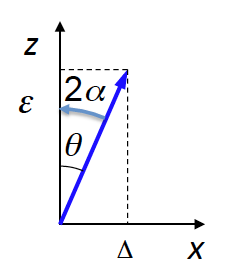
\includegraphics[height=4cm]{rot}
\end{figure}

\noindent

\noindent  Now  we perform  a  transformation  to  rotate the  state  by
$ 2\alpha = \theta $

  \begin{equation}
    \mathbf{U=e^{i\frac{\theta}{2}\sigma_y}} =  \cos(\alpha)\mathbb{I}+i\sin(\alpha)\sigma_y
  \end{equation}

  \noindent to rotate  the basis in this  plane.  \red{\textbf{Note that
      the transformation uses an angle HALF of the required turn}}.  The
  {time  independent  Hamiltonian}  will  be  transformed  according  to
  Eq.\eqref{uninewschrodinger},  and  evaluating using  the  commutation
  relations Eq.\eqref{uniComm1}

  \begin{equation}\label{uniRot}
    \begin{aligned}
      \mathcal{H}' & = U\mathcal{H}U^{\dagger} = U \bigg[-\frac{\Delta E}{2}\big(\sigma_z\cos(\theta)+\sigma_x\sin(\theta)\big)\bigg]\bigg[\cos(\theta/2)\mathbb{I}\red{-}i\sin(\theta/2)\sigma_y\bigg]\\
      & = U \bigg[\cos(\theta/2)\mathbb{I}+i\sin(\theta/2)\sigma_y\bigg]\bigg[-\frac{\Delta E}{2}\big(\sigma_z\cos(\theta)+\sigma_x\sin(\theta)\big)\bigg]\\
      & = UU\mathcal{H} =-\frac{\Delta E}{2} \bigg[\cos(\theta)\mathbb{I}+i\sin(\theta)\sigma_y\bigg]\bigg[\big(\sigma_z\cos(\theta)+\sigma_x\sin(\theta)\big)\bigg]\\
      & = -\frac{\Delta E}{2}\bigg[\cos^2(\theta)\sigma_z+\sin(\theta)\cos(\theta)\sigma_x+i\sin(\theta)\cos(\theta)\red{\sigma_y\sigma_z}+i\sin^2(\theta)\red{\sigma_y\sigma_x}\bigg]\\
      & = -\frac{\Delta E}{2}\bigg[\cos^2(\theta)\sigma_z+\sin(\theta)\cos(\theta)\sigma_x+i\sin(\theta)\cos(\theta)\red{i\sigma_x}+i\sin^2(\theta)\red{-i\sigma_z}\bigg]\\
      & = -\frac{\Delta E}{2}\sigma_z,
    \end{aligned}
  \end{equation}


  \noindent with  eigenstates $ \iket{\tilde{0}}, \iket{\tilde{1}}  $ at
  energies $  -\Delta E/2, +\Delta  E/2 $ respectively.   Recalling that
  the transformation we applied was

  \begin{equation}\label{uniTransform}
    \tilde{\Psi} = U\Psi \quad\Rightarrow\quad \Psi = U^{\dagger}\tilde{\Psi},
  \end{equation}

  \noindent in the initial eigenbasis, the two states will read

  \begin{equation}\label{uniInitial}
    \begin{aligned}
      \iket{0}_{\text{initial}}     &    =     U^{\dagger}\ket{\tilde{0}}    =
      \bigg(\cos(\theta/2)\mathbb{I}+i\sin(\theta/2)\sigma_y\bigg)\begin{pmatrix}
        1\\0
      \end{pmatrix} = \begin{pmatrix} \cos(\theta/2)\\\sin(\theta/2)
      \end{pmatrix} \\
      \iket{1}_{\text{initial}}      &       =      U^{\dagger}\ket{\tilde{1}}
      = \begin{pmatrix} -\sin(\theta/2)\\\cos(\theta/2)
      \end{pmatrix}.
    \end{aligned}
  \end{equation}


  \noindent  So ultimately,  rotating by  $ \theta/2  $ will  rotate the
  basis so as to cancel the interaction term.

 \subsection{Example application 2\label{subsec:Rabi}}
 Now  we have  a qubit  that  is driven  by a  resonant external  field,
 \red{this time  it is not  a $ \Delta $  intractions as the  strength varies
   with time}

  \begin{equation}\label{app2}
    \mathcal{H} = -\frac{\hbar\omega_0}{2}\sigma_z-\hbar\Omega\cos(\omega_0 t)\sigma_x
  \end{equation}

  \noindent for which we shall try the unitary transformation

  \begin{equation}\label{app2Try}
    U(t) = \exp\left[-i\frac{\omega_0 t}{2}\sigma_z\right]
  \end{equation}

  \noindent resulting in the Hamiltonian

  \begin{equation}\label{app2New}
    \begin{aligned}
      \mathcal{H'} & = U\mathcal{H}U^{\dagger} - i\hbar U\dot{U}^{\dagger}\\
      & = -\frac{\hbar\omega}{2}e^{-i\omega_0t/2\sigma_z}\sigma_ze^{+i\omega_0t/2\sigma_z}-\hbar\Omega\frac{e^{i\omega t}+e^{-i\omega t}}{2}e^{-i\omega_0t/2\sigma_z}\sigma_xe^{i\omega_0t/2\sigma_z}- i\hbar e^{-i\omega_0t/2\sigma_z}\bigg(i\frac{\omega}{2}\sigma_z\bigg)e^{i\omega_0t/2\sigma_z}\\
      & = -\frac{\hbar\Omega}{2}\bigg(e^{i\omega t}+e^{-i\omega t}\bigg)e^{-i\omega_0t/2\sigma_z}\red{e^{(-1)i\omega_0t/2\sigma_z}\sigma_x}\\
      & = -\frac{\hbar\Omega}{2}\bigg(e^{i\omega t}+e^{-i\omega t}\bigg){e^{-i\omega_0t\sigma_z}\sigma_x}\\
      &      =-\frac{\hbar\Omega}{2}\bigg(e^{i\omega      t}+e^{-i\omega
        t}\bigg)\begin{pmatrix} e^{-i\omega_0t}&0\\0&e^{+i\omega_0t}
      \end{pmatrix}\begin{pmatrix}
        0&1\\1&0
      \end{pmatrix}\\
      &      =-\frac{\hbar\Omega}{2}\bigg(e^{i\omega      t}+e^{-i\omega
        t}\bigg)\begin{pmatrix} 0&e^{i\omega_0t}\\e^{-i\omega_0t}&0
      \end{pmatrix}
      \\
      &                           =-\frac{\hbar\Omega}{2}\begin{pmatrix}
        0&1+e^{2i\omega_0t}\\1+e^{-2i\omega_0t}&0
      \end{pmatrix}
      \\
      & \approx -\frac{\hbar\Omega}{2}\begin{pmatrix} 0&1\\1&0
      \end{pmatrix}
      \\
      & \approx -\frac{\hbar\Omega}{2}\sigma_x
    \end{aligned}
  \end{equation}

  \noindent where we have applied the RWA where we neglect fast rotating
  terms \begin{framed}\noindent which correspond to non conserved energy
    processes
  \end{framed}                     qubit                     Hamiltonian
  ($ \mathcal{H} =  -\frac{\hbar\omega}{2}\sigma_z $), implicitly taking
  into  account the  raw evolution  to concentrate  only on  the driving
  field contribution.

  \begin{center}
    Coupling of levels via radiation = RWA.
  \end{center}

  Now the evolution of the state

  \begin{equation}\label{app2Ev}
    U(t) = e^{-i\mathcal{H'}/\hbar t} = e^{i\Omega t/2\sigma_x}
  \end{equation}

  \noindent gives according to Eq.\eqref{uniPauli}

  \begin{equation}\label{app2State}
    \ket{\Psi} = U\ket{0} = \cos(\frac{\Omega t}{2})\ket{0}+e^{i\pi/2}\sin(\frac{\Omega t}{2})\ket{1}.
  \end{equation}

\begin{figure}[h]
  \centering 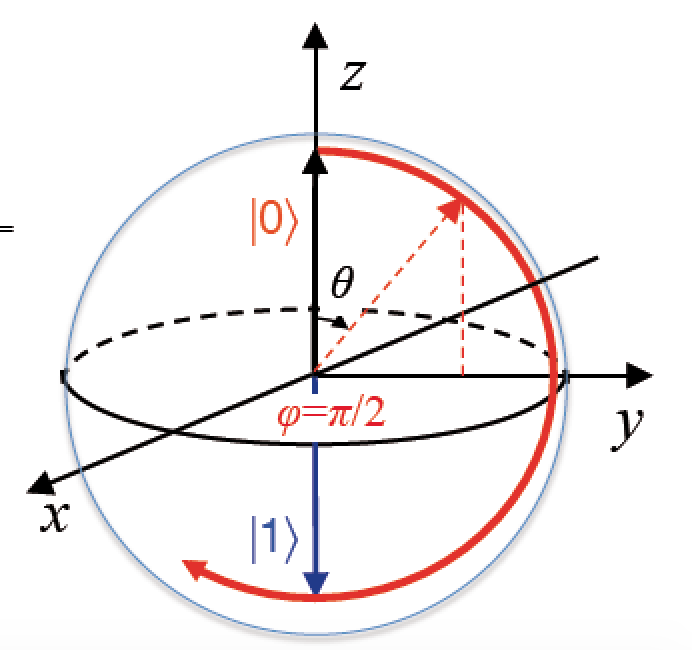
\includegraphics[height=2cm]{rotX}
\end{figure}

\noindent

\begin{framed}\noindent
  States  \iket{0}, \iket{1}  of the  same energy  (due to  the driving)
  interact with each other
\end{framed}
\noindent \textbf{It  may be  interesting to observe  the case  when the
  drive is changed}

  \begin{equation}\label{app2NewPhase}
    \hbar\Omega\cos(\omega t)\sigma_x \quad \rightarrow \quad \hbar\Omega\cos(\omega t+\mathbf{\phi})\sigma_x = \hbar\Omega\bigg[\cos(\omega t)\cos(\phi)-\sin(\omega t)\sin(\phi)\bigg]\sigma_x
  \end{equation}

  \noindent for which  the procedure for the cosine part  using the same
  unitary transformation Eq.\eqref{app2Try} gives

  \begin{equation}\label{app2Cos}
    -\frac{\hbar\Omega}{2}\cos(\phi)\sigma_x,
  \end{equation}

  \noindent                           while                          the
  $ \sin(\omega t) = i(e^{i\omega t}-e^{-i\omega t})/2 $ gets

  \begin{equation}\label{app2Sin}
    -\frac{\hbar\Omega}{2}\sin(\phi)\sigma_y,
  \end{equation}

  \noindent giving

  \begin{equation}\label{app2Combined}
    \mathcal{H'} = -\frac{\hbar\Omega}{2}\bigg(\sigma_x\cos\phi+\sigma_y\sin\phi\bigg)
  \end{equation}


 \subsection{Qubit operations}
 In the previous section, the qubit system was subjected to a field that
 induced rotation about  the x-axis.  In a similar way,  one can perform
 qubit operations about other axes

 {\footnotesize \begin{table}[h]
     \begin{center}
       \begin{tabular}{|c|c|c|c|c|}
         \hline \textbf{Axis} & \textbf{Field operator $ \mathcal{H} $} & \textbf{Unitary evolution}$ U=\exp\left[i\mathcal{H}t/\hbar\right] $ & $ \mathbf{t=\frac{\pi}{\Omega}} $& $ \mathbf{t=\frac{\pi}{2\Omega}} $\\
         X&$ -\frac{\hbar\Omega}{2}\sigma_x $ & $ \begin{pmatrix}
           \cos{\Omega t/2} & -i\sin{\Omega t/2}\\-i\sin{\Omega t/2}&\cos{\Omega t/2}
         \end{pmatrix} $ & NOT = $\begin{pmatrix} 0 & -i \\-i&0
         \end{pmatrix} $ &\\
         Y&$         -\frac{\hbar\Omega}{2}\sigma_y          $         &
                                                $ \begin{pmatrix} \cos{\Omega
                                                    t/2}    &    -\sin{\Omega
                                                           t/2}\\\sin{\Omega
                                                    t/2}&\cos{\Omega t/2}
                                                \end{pmatrix}
                                                          $ &  FLIP =
                                                              $\begin{pmatrix}
                                                                0   &  -1
                                                                \\1&0
                                                              \end{pmatrix}
                                                                     $  &   H  =
                                                                          $
                                                                          \frac{1}{\sqrt{2}}\begin{pmatrix}
                                                                            1   &  -1
                                                                            \\1&1
                                                                          \end{pmatrix} $\\
         Z&$         -\frac{\hbar\Omega}{2}\sigma_z          $         &
                                                $        \begin{pmatrix}
                                                    e^{-i\Omega  t/2}  &
                                                                       0\\0&e^{i\Omega
                                                                             t/2}
                                                                         \end{pmatrix}
                                                                             $&$\begin{pmatrix}
                                                                               -i&0\\0&i
                                                                             \end{pmatrix}$&\\\hline
       \end{tabular}
     \end{center}
   \end{table}}
 \newpage
%
\section{Dissipation\label{sec:linbland1}}
 In this chapter we will ultimately look to understand the image below, which describes the dissipation processes that can occur in a two levels system
 
 \begin{figure}[h]
 	\ifigure{5cm}{cohereneUnd}
 \end{figure}

 In all of the calculation we shall use the density matrix representation in order to represent mixed states that form in a system. Important properties of density matrices are:
 
 \begin{itemize}
 	\item \textbf{Diagonal - off diagonal connection for pure state}
 	
 	\begin{equation}\label{dOffD}
 		\rho=\ketbra{\psi}{\psi} = \begin{pmatrix}
 			\alpha\\\beta
 		\end{pmatrix}\begin{pmatrix}
 			\alpha^{*}&\beta^{*}
 		\end{pmatrix} = \begin{pmatrix}
	 		|\alpha|^2&\alpha\beta^{*}\\\alpha^{*}\beta&|\beta|^2
 		\end{pmatrix} \Rightarrow \red{|\rho_{01}|^2 = \rho_{00}\rho_{11}}
 	\end{equation}
 	\item \textbf{Sum} of the diagonal elements
 	
 	\begin{equation}\label{sum}
 		\red{\rho_{00}+\rho_{11}=1}
 	\end{equation}
 	\item \textbf{Some common expectation values}
 	
 	\begin{equation}\label{expectation}
 		\begin{aligned}
	 		\iaverage{\sigma_z} &= \itrace{\begin{pmatrix}
	 			\rho_{00}&\rho_{01}\\\rho_{10}&\rho_{11}
	 			\end{pmatrix}\begin{pmatrix}
	 			1&0\\0&-1
	 			\end{pmatrix}} = \itrace{\begin{pmatrix}
	 				\rho_{00}&-\rho_{01}\\\rho_{10}&-\rho_{11}
	 			\end{pmatrix}} = \rho_{00}-\rho_{11}; \\
 			&\red{\rho_{11} = \frac{1-\iaverage{\sigma_z}}{2}};\quad \quad \red{\rho_{00} = \frac{1+\iaverage{\sigma_z}}{2}}\\
				\iaverage{\sigma_x} &=  \rho_{01}+\rho_{10}\\
				\iaverage{\sigma_y} &=  i\rho_{01}-i\rho_{10}\\
				\iaverage{\sigma_{+}} &= \frac{\iaverage{\sigma_x}+i\iaverage{\sigma_y}}{2} = \rho_{10}\\
				\iaverage{\sigma_{-}}& = \frac{\iaverage{\sigma_x}-i\iaverage{\sigma_y}}{2} = \rho_{01}\\
 		\end{aligned}
 	\end{equation}
 	
 	\item \textbf{Evolution} is governed by the Von-Neumann equation
 	
 	\begin{equation}\label{vonN}
 		i\hbar\dot{\rho} = \bigg[\mathcal{H},\rho\bigg]
 	\end{equation} 
 	
 	\noindent a simple two level system, $ \mathcal{H} = -\hbar\omega\sigma_z/2 $ giving rise to 
 	
 	\begin{equation}\label{key}
 	\begin{aligned}
 		i\hbar
 			\begin{pmatrix}
	 			\dot{\rho_{00}} & \dot{\rho_{01}}\\\dot{\rho_{10}}&\dot{\rho_{11}} 
	 		\end{pmatrix} 
	 	& = -\frac{\hbar\omega}{2}
	 		\begin{pmatrix}
	 			1 & 0\\0&-1
	 		\end{pmatrix}
	 		\idensity + \frac{\hbar\omega}{2}\idensity\iz \\
	 	& = {-i\omega}{}
	 		\begin{pmatrix}
	 			0 & -\rho_{01}\\-\rho_{10}&0
	 		\end{pmatrix}\\\\
	 	\rho_{00} = &\rho_{00}(0);\quad\rho_{11}(t) = \rho_{11}(0);\quad\rho_{01}(t) = \rho_{01}(0)e^{i\omega t};\quad\rho_{10}(t) = \rho_{10}(0)e^{i\omega t}
 	\end{aligned}
 	\end{equation} 
 \end{itemize}

 \red{This is rotation about the equator of the Bloch sphere.}
 \subsection{Application to relaxation} 
  Now, if we excite the system, we will inevitably observe a decay to the ground state - the probability of the system being in an excited states exponentially decreases
 
 \begin{equation}\label{relaxationRaw}
 	 \frac{d\rho_{11}}{dt}=-\rho_{11}\frac{1}{T} =  -\rho_{11}\Gamma_1\quad\Rightarrow\quad\rho_{11} = \rho_{11}(0)e^{-t/T}.
 \end{equation}
 
 \noindent Such a relaxation will eventually lead to the state of the system to change to a mixed state
 
 \begin{equation}\label{relax2}
 	\rho(0) = \ketbra{1}{1} = \imx{0}{0}{0}{1}_{\red{\text{pure}}} \iright \rho(t=T\ln2) =\imx{\frac{1}{2}}{0}{0}{\frac{1}{2}}_{\red{\text{mixed}}},
 \end{equation}
 
 \noindent which in terms of probabilities has the \textbf{exact same properties} as
 
 \begin{equation}\label{relax3}
 	\rho = \imx{1}{1}{1}{1}_{\red{\text{pure}}}.
 \end{equation}
 
 \noindent The state in Eq.\eqref{relax2} has lost coherence as the system underwent relaxation. The system that was initially in a pure state {when \red{$ |\rho_{01}(0)|^2=\rho_{00}(0)\rho_{11}(0) $}} to a mixed state when \red{$ |\rho_{01}(t)|^2\le\rho_{00}(t)\rho_{11}(t) $}. The off diagonal terms loose information and tend to zero. 
 
 This is accounted for by writing the Linbland term
 
 \begin{equation}
 \dot{\rho} = \frac{-i}{\hbar}\bigg[\mathcal{H},\rho\bigg] + \mathcal{L};\quad\quad\mathcal{L} = \begin{pmatrix}
 \blue{\rho_{11}\Gamma_1 }& \red{-\Gamma_2\rho_{01}}\\\red{-\Gamma_2\rho_{01}}&\blue{-\Gamma_1\rho_{11}}
 \end{pmatrix}, 
 \end{equation}
 
 \begin{itemize}
 	\item \textbf{\blue{Relaxation}} will cause $ \rho_{00} $ to increase and $ \rho_{11} $ to decrease
 	\item \textbf{\red{Pure dephasing}} - its is well known that the diagonal elements of a density matrix \textbf{must} obey
 	\begin{equation}\label{pd1}
 		|\rho_{01}|^2\le\rho_{00}\rho_{11},
 	\end{equation}
 	
 	\noindent equality being achieved for a pure state. During relaxation $ \rho_{00} $ increases and $ \rho_{11} $ decreases, but as relaxation can only decrease coherence, it is only the latter term that will effect off diagonal elements
 	
 	\begin{equation}\label{pd2}
 		\ialigned{\delta|\rho_{01}| & \le \sqrt{\rho_{00}(\rho_{11}+\delta\rho_{11})} - \sqrt{\rho_{00}\rho_{11}}\\
 		\delta\rho_{11} & = -\rho_{11}\Gamma_1dt\quad\text{from Eq.\eqref{relaxationRaw}}}\iright\ialigned{\delta|\rho_{01}|&\le\sqrt{\rho_{00}\rho_{11}}\bigg(\sqrt{1-\Gamma_1dt}-1\bigg)\\&\approx\sqrt{\rho_{00}\rho_{11}}\bigg(-\frac{\Gamma_1}{2}dt\bigg)\\&\red{ = -|\rho_{01}\frac{\Gamma_1}{2}dt}},
 	\end{equation}
 	
 	\noindent meaning that the decay of the off diagonal terms cannot be slower than $ \frac{\Gamma_1}{2} $. Taking into account other ways of diagonal terms dephasing, $ \Gamma_\phi $, one assigns 
 	
 	\begin{equation}\label{pd3}
 		\Gamma_2 = \frac{\Gamma_1}{2}+\Gamma_\phi;\quad T_2 = \frac{1}{\Gamma_2}
 	\end{equation}
 \end{itemize}

	\iframe{\red{This is a very crude argument, and possibly a coincidence. Nevertheless, the required $ \Gamma_2 $ factos is distilled.}}
 
 \subsection{Pure dephasing}
  Attention will now be direct to the $ \Gamma_2 $ term introduced in Eq.\eqref{pd3}, and more specifically its pure dephasing component $ \Gamma_\phi $. Pure dephasing is due to noise that affects the separation of the qubit energy levels. Recall from Sec.~\ref{subsec:Rabi}, that a qubit system that is subjected to a resonant driving field (whose frequency, $ \omega $, matches the energy separation, $ \hbar\omega_0 $, of the levels)
  
  \begin{equation}\label{RabiHamiltonian}
  	\mathcal{H} = -\frac{\hbar\omega_0}{2}\sigma_z-\hbar\Omega\cos(\omega_0 t)\sigma_x,
  \end{equation}
  
  \noindent will, in the RWA, evolve from an initial state \iket{0} according to
  
  \begin{equation}\label{RabuSolution}
  	\ket{\Psi} = U\ket{0} = \cos(\frac{\Omega t}{2})\ket{0}+e^{i\pi/2}\sin(\frac{\Omega t}{2})\ket{1}.
  \end{equation}
  
  \noindent Should the separation of the levels vary, $ \hbar\omega_0 \rightarrow \hbar\omega' $, then the qubit will be in resonance with another component of the driving field, $ \hbar\Omega'\cos(\omega't)\sigma_x $, meaning that the evolved state will be a superposition of the form
  
  \begin{equation}\label{RabuSolutionSuperpos}
  	\iket{\Psi} = \sum_i \alpha_i\bigg[\cos\bigg(\frac{\Omega_i t}{2}\bigg)\iket{0}+i\sin\bigg(\frac{\Omega_i t}{2}\bigg)\iket{1}\bigg],
  \end{equation}
  
  \noindent leading to a probability of observing the system in \iket{0} of
  
  \begin{equation}\label{RabiProb0}
  	P_0  = |\bra{0}\iket{\Psi}|^2 = \sum_i \alpha_i\cos^2\bigg(\frac{\Omega_it}{2}\bigg)=\quad \left\lbrace \text{ equal weights for 3 states}\right\rbrace \quad= \frac{1}{3}\bigg(\cos^2\bigg(\frac{\Omega_1t}{2}\bigg)+\cos^2\bigg(\frac{\Omega_2t}{2}\bigg)+\cos^2\bigg(\frac{\Omega_3t}{2}\bigg)\bigg),
  \end{equation}
  
  \noindent which leads to a probability 'averaging' as one monitors the system for longer times $ t $, the characteristic decay time being labelled as$ T_\phi =1/\Gamma_\phi $. The Rabi oscillations are `washed out' due to this dephasing. The bigger the fluctuations of the energy levels the stronger the washing out. If one hopes to observe any oscillations, then the Rabi frequency $ \Omega>>1/T_\phi = \Gamma_2 $ to ensure that oscillation occur before dying off.
  
  \begin{figure}
  	\ifigure{4cm}{deph1}
  	\ifigure{4cm}{deph2}
  \end{figure}
 
 \newpage
 
 \subsection{Dynamics with Pauli Matrices\label{subsec:dynamics_with_pauli}}
  Summarising up to this point, we have argued for the appearance of the Linbland term in the Master equation to account for decoherence and relaxation processes in the system 
 \red{{\large  \begin{equation}\label{Totalequation}
  	\mathcal{L} = \imx{\Gamma_1\rho_{11} - \Gamma^{ex}\rho_{00}}{-\Gamma_2\rho_{01}}{-\Gamma_2\rho_{10}}{\Gamma^{ex}\rho_{00}-\Gamma_1\rho_{11}};\quad \dot{\rho} = -\frac{i}{\hbar}\big[\mathcal{H},\rho\big]+\mathcal{L},
  \end{equation}}}
  
  \noindent and shown a few useful expectation values, that allow one to express the dynamics of the system via the expectation values of the Pauli matrices, Eq.\eqref{expectation}
  
  \red{{\large \begin{equation}\label{expectationPauli}
  	\rho_{00} = \frac{\iaverage{\sigma_z}+1}{2};\quad \rho_{01}=\frac{\iaverage{\sigma_x}-i\iaverage{\sigma_y}}{2} = \iaverage{\sigma_{+}};\quad\rho_{10}=\frac{\iaverage{\sigma_x}+i\iaverage{\sigma_y}}{2} = \iaverage{\sigma_{-}};\quad\rho_{11} = \frac{1-\iaverage{\sigma_z}}{2}.
  \end{equation}
  \begin{equation}\label{expectationPauli2}
  	\iaverage{\sigma_x}=\rho_{01}+\rho_{10};\quad\iaverage{\sigma_y} = i\rho_{01}-i\rho_{10};\quad\iaverage{\sigma_z}=\rho_{00}-\rho_{11}
  \end{equation}}}
  
  \noindent Lets compute the evolution of these expectation values
  
  \begin{equation}\label{evolution}
  	\ialigned{\difffrac{\iaverage{\sigma_j}}{t}&=\itrace{\sigma_j\difffrac{\rho}{t}} = \itrace{-\frac{i}{\hbar}\sigma_j\big(\mathcal{H}\rho - \rho\mathcal{H}\big)+\sigma_j\mathcal{L}}\\
  	\mathcal{H}&  = \frac{\hbar\Omega}{2}\bigg(\sigma_x\cos(\phi)-\sigma_y\sin(\phi)\bigg),}
  \end{equation}
  
  \noindent and evaluating for all the matrices
  
  \begin{equation}\label{pauliDeriv}
  	\begin{aligned}
  	\difffrac{\iaverage{\sigma_x}}{t}&=-i\frac{\Omega}{2}\itrace{\cancel{\big(\sigma_x\sigma_x\rho-\sigma_x\rho\sigma_x\big)}\cos(\phi) + \big(\sigma_x\sigma_y\rho-\sigma_x\rho\sigma_y\big)\sin(\phi)} + \itrace{\sigma_x\mathcal{L}}\\
  	& = \Omega\iaverage{\sigma_z}\sin(\phi)-\Gamma_2\iaverage{\sigma_x}\\
  	\difffrac{\iaverage{\sigma_y}}{t}& = \Omega\iaverage{\sigma_z}\sin(\phi)-\Gamma_2\iaverage{\sigma_y}\\
  	\difffrac{\iaverage{\sigma_y}}{t}& = -\Omega\big(\iaverage{\sigma_x}\cos(\phi)+\iaverage{\sigma_y}\sin(\phi)\big)-\Gamma_1\iaverage{\sigma_z}+\Gamma_1\\
  	\end{aligned}
  \end{equation}
  
  \noindent or in more compact form
  
  \begin{equation}\label{pauliEv}
  	\difffrac{}{t}\begin{pmatrix}
  		\iaverage{\sigma_x}\\\iaverage{\sigma_y}\\\iaverage{\sigma_z}
  	\end{pmatrix} = \begin{pmatrix}
	  	-\Gamma_2&0&\Omega\sin(\phi)\\0&-\Gamma_2&\Omega\cos(\phi)\\-\Omega\sin(\phi)&-\Omega\cos(\phi)&-\Gamma_1\\
  	\end{pmatrix}\begin{pmatrix}
  	\iaverage{\sigma_x}\\\iaverage{\sigma_y}\\\iaverage{\sigma_z}
  	\end{pmatrix}+\begin{pmatrix}
  	0\\0\\\Gamma_1
  	\end{pmatrix}\iright\red{\difffrac{\vec{\iaverage{\sigma}}}{t} = B\vec{\iaverage{\sigma}}+\vec{b}.}
  \end{equation}
  
  \noindent The dynamics of this system are the exact same as for a spin 1/2 particle in a magnetic field \textbf{B} studied in Chapter \ref{spin12} Eq.~\eqref{eqn:evolutionBloch}. The different components of the vector \isigma can be plotted on a sphere. Note that unlike the Bloch sphere used previously, these vectors do \textbf{not} have to be on the surface. The various states $ \vec{\iaverage{\sigma}} $ correspond to
  
  \begin{align}
  	\rho_{00}=1 & \iright \isigma = \ithreeMatrix{0}{0}{1}\\
  	\rho_{11}=1 & \iright \isigma = \ithreeMatrix{0}{0}{-1}\\
  	\rho_{00}=\rho_{11}&\iright\isigma = \ithreeMatrix{\cos(\phi)}{\sin(\phi)}{0}
  \end{align}
  
  \begin{figure}[h]
  	\ifigure{7cm}{sphere}
  \end{figure}

	\newpage
	
 \paragraph{Starting in the superposed state}
 
 So now let us study some dynamics, where, unless specified, we take the initial state to be $ \rho_{00}=1/2 $ i.e. on the equator where the atom has equal occupation in levels \iket{0} and \iket{1}. An general state would be
 
 \[
 	\Psi = \frac{\iket{0}+e^{i\phi}\iket{1}}{\sqrt{2}} \quad\ra\quad \rho = \frac{1}{2}\imatrix{1}{e^{-i\phi}}{e^{i\phi}}{1}
 \]
 
 \begin{itemize}
 	\item \textbf{\red{No driving} No decoherence} - the superposed state will remain superposed.
 	\[	
	 	\begin{aligned}
	 	\mathcal{H} = -\frac{\hbar\omega}{2}\sigma_z &\iRa  U = \imatrix{e^{i\omega t}}{0}{0}{e^{-i\omega t}}\\
	 	&\iRa \rho(t) = U\rho(0)U\idagger = \frac{1}{2}\imatrix{e^{i\omega t}}{e^{i(\omega t - \phi)}}{e^{-i(\omega t - \phi)}}{e^{-i\omega t}}\imatrix{e^{-i\omega t}}{0}{0}{e^{+i\omega t}}\\
	 	&\qquad \qquad\qquad\qquad\red{= \frac{1}{2}\imatrix{1}{e^{i(2\omega t - \phi)}}{e^{-i(2\omega t - \phi)}}{1}}
	 	\end{aligned}
 	\]
 	
 	\red{But when we consider the situation from by entering the rotating frame (the interaction picture), see Chapter~\ref{sec:unitary} and Ch.~\ref{sec:interaction}}
 	
 	\[
 		U_0(t) = e^{i\frac{\mathcal{H}_0}{\hbar}t},	
 	\]
 	
 	\noindent the interaction picture Hamiltonian will be of the form Eq.~\eqref{eqn:interactionPictureHamiltonian}
 	
 	\[
 		\mathcal{H}_i = U_0(t)\idagger\bigg[\mathcal{H} - \mathcal{H}_0\bigg]U_0(t) \equiv 0,
 	\]
 	
 	\noindent and so there will be no evolution in the system in this rotated frame that we work with. The expectation values, \isigmax, \isigmaz are the same as in the rotated and non-rotating frames:
 	
 	\begin{equation}
 	_I\bra{\psi}\hat{O}_I\ket{\psi}_I = _S\bra{\psi}U_0U_0^\dagger\hat{O}_SU_0U_0^\dagger\ket{\psi}_s \equiv _S\bra{\psi}\hat{O}_S\ket{\psi}_S
 	\end{equation}
 	
 	\ipic{4cm}{doD2}
 	\ipicCaption{4cm}{doD1}{On the equator the atom has equal weight in \iket{0} and \iket{1}, so \isigmaz is 0. The \isigmax is stationary.}

 	
 
 	\newpage
 	\item \textbf{\red{Driving} No decoherence, $ \Gamma_1 = 0, \Gamma_2 = 0 $}
 	
 	We evolution of the wavefunction is taken to be \red{under a drive from a resonant field}
 	
 	\begin{equation}\label{dunamicState}
 	\ket{\Psi} = \cos\big(\frac{\Omega t}{2}\big)\ket{0}+i\sin\big(\frac{\Omega t}{2}\big)\ket{1};\quad\rho=\ketbra{\Psi}{\Psi}
 	\end{equation}
 	
 	
 	\begin{equation}\label{dyn1}
 		\ialigned{
 			\rho_{11} & = \sin^2(\Omega t/2) & \iaverage{\sigma_x} & = \rho_{01}+\rho_{10} = \sin(\Omega t)\\
 			\rho_{01} & = \sin(\Omega t/2)\sin(\Omega t/2) = \frac{\sin(\Omega t)}{2} & \iaverage{\sigma_y} & = i\rho_{01}-i\rho_{10} = 0\\
 			\rho_{10} & = \sin(\Omega t/2)\sin(\Omega t/2) = \frac{\sin(\Omega t)}{2} & \iaverage{\sigma_z} & = 1- 2\rho_{00} = \cos(\Omega t)\\
 		}
 	\end{equation}
 	
 	\noindent and the point on the sphere simply rotates about the \iaverage{\sigma_y} axis. If there was a phase shift in the driving field $ \phi $ then the rotation would turn by that angle about the \iaverage{\sigma_z} axis. Overall these are the Rabi oscillations
 	
 	\begin{figure}[h]
 		\ifigure{4cm}{dyn1}
 		\ifigure{4cm}{dnO}
 	\end{figure}
 
  	\newpage
   \item \textbf{\textbf{\red{Driving} With decoherence $ \Gamma_1 = 1, \Gamma_2 = 0.5, \gamma = \Gamma_1+\Gamma_2/2 $}}, it is simpler to solve the dynamics of Eq.\eqref{pauliEv} for \iaverage{\vec{\sigma}}
   
   For the case when one starts off with state $ \rho_{00} = 1 $
   
   \begin{equation}\label{dyn2}
   \ialigned{
   	\iaverage{\sigma_x} & \approx e^{-\gamma t} \sin(\Omega t) & \rho_{00} & = \frac{\iaverage{\sigma_z}+1}{2} \approx\frac{1+e^{-\gamma t} \cos(\Omega t)}{2}\\
   	\iaverage{\sigma_y} & = 0 & \rho_{01} & = \frac{\iaverage{\sigma_x}-i\iaverage{\sigma_y}}{2} = \frac{e^{-\gamma t} \sin(\Omega t)}{2}\\
   	\iaverage{\sigma_z} & \approx e^{-\gamma t} \cos(\Omega t) & \rho_{10} & = \frac{\iaverage{\sigma_x}+i\iaverage{\sigma_y}}{2} = \frac{e^{-\gamma t} \sin(\Omega t)}{2}\\
   }
   \end{equation}
   
   \noindent In this case the two components begin to spiral in as a result of the dephasing. The central point is the stationary condition in which both \iaverage{\sigma_x} and \iaverage{\sigma_z} take on a finite value - the stationary state value. 
   
   \begin{figure}[h]
   	\ifigure{6cm}{dyn2}
   	\ifigure{5cm}{dd}
   \end{figure}

	\newpage
   \item \textbf{\red{No driving} with decoherence and relaxation} $ \rho_{00}=\rho_{11} = 1/2 $ then
   
   \begin{equation}\label{dyn21}
   	\ialigned{
   	\iaverage{\sigma_x} & = e^{-\Gamma_2 t} & \rho_{00} & = 1-\frac{e^{-\Gamma_1 t}}{2}\\
   	\iaverage{\sigma_y} & = 0 & \rho_{01} & = \frac{e^{-\Gamma_2 t}}{2} \\
   	\iaverage{\sigma_z} & = 1 - e^{-\Gamma_1 t} & \rho_{10} & = \frac{e^{-\Gamma_2 t}}{2} \\
   }
   \end{equation}
   
   The system, initially on the `equator' of the sphere, transitions to the ground state
   
     \begin{figure}[h]
   	\ifigure{6cm}{dyn21}   	
   	\ifigure{6cm}{dyn22}
   \end{figure}
   
   \newpage
   \item \textbf{\red{No driving} Only dephasing $ \Gamma_1=0, \Gamma_2 \ne 0 $} when we start off in a superposed state $ \rho_{11}=1/2\rightarrow\iaverage{\sigma_z}=0 $
   
   \begin{equation}\label{dyn3}
   \ialigned{
   	\iaverage{\sigma_x} & = e^{-\Gamma_2 t} & \rho_{00} & = \frac{1}{2}\\
   	\iaverage{\sigma_y} & = 0 & \rho_{01} & = \frac{e^{-\Gamma_2 t}}{2} \\
   	\iaverage{\sigma_z} & = 0 & \rho_{10} & = \frac{e^{-\Gamma_2 t}}{2} \\
   }
   \end{equation}
   
   The expectation value simply moves towards the origin, where $ \iaverage{\sigma_z} = 0 $ and the system becomes equally likely to exist in the excited or ground state $ \rho_{00}=\rho_{11} $. The off diagonal terms loose coherence.
   
   \begin{figure}[h]
   	\ifigure{6cm}{dyn31}
   	\ifigure{4cm}{nd1}
   \end{figure}
 \end{itemize}
  
 {\large \red{\textbf{Thus, relaxation will tend to shift \iaverage{\sigma_z} to 1, and together with pure dephasing it shortens the expectation values of the \iaverage{\sigma_x} and \iaverage{\sigma_y} directions.}}}
\newpage%
% -*- TeX-master: "../all_the_notes.tex" -*-

\section{Linbalnd operators covered in depth\label{sec:linbland2}}
This  section  will  cover  how  we  derive  these $  L_j  $  operators  which  were  used  in
Sec.~\ref{subsec:dynamics_with_pauli}.
\subsection{Pure dephasing\label{sec:lin_1}}
Let us consider a two level system, whose  Hamiltonian is undergoing a fluctuation in time due
to \red{movement of the energy levels}
\begin{equation}\label{eq:lin_2}
  \mathcal{H} = \imatrix{\red{\epsilon(t)}}{0}{0}{0} \iratext{eigenstates} \ialigned{\iket{0} & = \imatrixcol{0}{1}\\\iket{1} & = \imatrixcol{1}{0}}.
\end{equation}
  
\noindent Under  free evolution an  arbitrary state \iket{\Psi(0)}  = a\iket{1} +  b\iket{0} will
evolve to:
  
\begin{equation}\label{eq:lin_3}
  \begin{aligned}
    \iket{\Psi(t)} & = \prod_i U(\Delta t_i) \iket{\Psi(0)} \\
    & = \prod_i \exp\left[-i\frac{\epsilon(\Delta t_i)}{\hbar} \imatrix{1}{0}{0}{0}\right]\imatrixcol{a}{b}\\
    & = \prod_i \bigg(\mathbb{I}\imatrixcol{a}{b} + \blue{\sum_{{N = 1}}\frac{\left[\frac{-i\epsilon(\Delta t_i)}{\hbar}\right]^N}{N!} \imatrix{1}{0}{0}{0}\imatrixcol{a}{b}}\bigg)\\
    & = \prod_i \bigg(\imatrixcol{a}{b} + \blue{\exp\left[-i\frac{\epsilon(\Delta t_i)}{\hbar}\right]\imatrixcol{a}{0} - \imatrixcol{a}{0}\bigg)}\\
    & = \prod_i \imatrixcol{e^{-i\frac{\epsilon(\Delta t_i)}{\hbar}}a}{b} = \imatrixcol{e^{-i\sum_i\frac{\epsilon(\Delta t_i)}{\hbar}}a}{b} \\
    & \red{= \imatrixcol{ae^{i\varphi}}{b} \qquad \varphi = -\int_{0}^{t}\frac{\epsilon(t')}{\hbar}dt'}
  \end{aligned}
\end{equation}
 
\iframe{\noindent  Thus, free  evolution  under a  fluctuating  energy will  lead  to a  phase
  accumulation between the two states:
  \begin{equation}\label{eq:lin_4}
    \ket{\Psi} = a\red{e^{i\varphi}}\iket{1} + b\iket{0} =  \imatrixcol{a\red{e^{i\varphi}}}{b}
  \end{equation}
 		
  \noindent which we  can probe by measuring  the \isigmax\ component and  see this integrated
  phase:
 		
 		\begin{equation}\label{eqn:lin_1}
                  \isigmax = ab^{*}\red{e^{i\varphi}} + a^{*}b\red{e^{-i\varphi}} \iratext{a,b real} 2ab\cos(\varphi).
 		\end{equation}
              }
 
              \newpage
              \paragraph{Single run}  Each measurement  of $  \sigma_x $ gives  $ \pm1  $ with
              probabilities (projecting onto the respective eigensubspaces):
  
              \begin{equation}\label{eq:linrelax_8}
                \begin{aligned}
                  &P(1) = \iabsSquared{\bra{\Psi}\left(\frac{\iket{0} + \iket{1}}{\sqrt{2}}\right)} = \frac{1}{{2}}\iabsSquared{ae^{-i\varphi} + b} = \frac{1}{2}\left({a}^2 + {b}^2 + 2ab\cos(\varphi) \right)\\
                  & P(-1) = \frac{1}{2}\left(a^2 + b^2 - 2ab\cos(\varphi)\right)
                \end{aligned}
              \end{equation}
    
              \ipicCaption{3cm}{lin_1}{The  energy  of the  two  levels  fluctuates around  0.
                Integration       will       give       a      unique       phase       value,
                $ \phi  = -\int_0^t\frac{\epsilon(t')}{\hbar}dt'  $, that  determines collapse
                probability. \textbf{This is for a single run.}}
  
              \paragraph{Averaging} Averaging over the $ \pm 1  $ will allow us to recover the
              \isigmax $ \propto \cos(\varphi) $ dependence.
              \begin{itemize}
              \item  Each run  has an  independent $  \epsilon(t) $  and hence  an independent
                $ e^{i\varphi} $;
              \item    Averaging    will    thus    result   in    the    classical    average
                \iaverage{e^{i\varphi}}$ _\varphi $.
              \end{itemize}

              \iframe{\noindent And thus Eq.~\eqref{eqn:lin_1} will in practise be reading:
  
  \begin{equation}\label{eq:linrelax_10}
    \isigmax = ab^{*}\blue{\iaverage{e^{i\varphi}}_\varphi} + a^{*}b\iaverage{e^{-i\varphi}}_\varphi \iratext{a,b real} 2ab\cos(\iaverage{\varphi}_\varphi).
  \end{equation}}
  
\noindent Let us label this interference term factor
  
  \begin{equation}\label{eq:linrelax_11}
    v(t) = \blue{\iaverage{e^{i\varphi}}_\varphi},
  \end{equation}
  
  \noindent   which    is   reflective    of   the    noise   supression    of   interference:
  $ \blue{v(t)} \ra 0 $.
  
  \ipicCaption{3cm}{lin_2}{The longer we  allow the phase, $ \varphi $,  to evolve the greater
    amount  of cancellation  between the  independent  runs we  shall  get.  In  this way  and
    interference that we can infer will wash out.\label{fig:lin_2}}
  
  \noindent  \red{\paragraph{Why does  it decrease  with  time?}  Making  the assumption  that
    $ \epsilon(t) $ fluctuates around 0 we will find that %$ \varphi $ can be expanded:
  	
    % \begin{equation}\label{key}
    %             \iaverage{\varphi(t)}_\varphi           =
    %             \iaverage{\varphi(0)}_\varphi           +
    %                 %             t\iaverage{\difffrac{\varphi}{t}|_{t=0}}_\varphi
    %                 %             +
    %                 %             \frac{t^2}{2}\iaverage{\difffrac{^2\varphi}{t^2}|_{t=0}}_\varphi
    %                 %             + \cdots
    % \end{equation}
%  	
    % \noindent and because
    \begin{itemize}
    \item Initially any $ \varphi(0)  = -\int_{0}^{0}\frac{{\epsilon(t')}}{\hbar}dt' = 0 $ (no
      phase has been allowed to accumulate) and therefore
      \begin{equation}\label{key}
        \iaverage{e^{i\varphi(0)}}_\varphi = 1.
      \end{equation}
    \item Subsequently, the random evolution of the phase will lead to
  		
      \begin{equation}\label{key}
        \begin{aligned}
          \iaverage{e^{i\varphi(t)}}_\varphi & = e^{i\phi_1(t)} + e^{i\phi_2(t)} + e^{i\phi_3(t)} + \cdots\\
          & = x_1 + iy_1 + x_2 + iy_2 + x_3 + iy_3 + \cdots\\
          & = \iaverage{x} + i\iaverage{y}\\
          & = 0 + i0 = 0
        \end{aligned}
      \end{equation}
  		
      \noindent and thus perfect cancellation - any agreement between the states will persists
      only for short times.
    \end{itemize}}
 
 \subsection{Pure dephasing from partial trace\label{sec:lin_2}}
 We can  arrive at  Eq.~\eqref{eqn:lin_1} in  a similar fashion  by considering  a system-bath
 state
   
   \begin{equation}\label{key}
     \ket{\Psi_{SB}} = \ket{\Psi} \otimes \ket{\chi_B} \quad\text{where}\quad 
     \ialigned{
       \Ket{\Psi} & = a\iket{1} + b\iket{0}\\
       \ket{\chi} & = \sum_i\sqrt{w_i}\ket{\chi_j}
     } 
   \end{equation}
  
   \noindent where the bath is a weighted superposition of \iket{\chi_i} states (normalised of
   course).
  
   \iframe{\noindent We postulate, that  the state of the system will  evolve acoording to the
     state of the bath:
     \begin{equation}\label{key}
       \begin{aligned}
         U_{SB}(t)\iket{1}\ket{\chi_i} & = \red{e^{i\varphi_i(t)}}\iket{1}\ket{\chi_i}\\
         U_{SB}(t)\iket{0}\ket{\chi_i} &=\iket{0}\ket{\chi_i}\\
       \end{aligned}
     \end{equation}
     \noindent acquiring a  phase only for the  \iket{1} state and depending on  the states of
     the bath.  }

   \noindent Thus we shall get the following evolution:
   \begin{equation}\label{key}
     \begin{aligned}
       \ket{\Psi_{SB}(t)} & = aU_{SB}(t)\left[\sum_i\sqrt{w_i}\ket{1}\ket{\chi_i}\right] + bU_{SB}(t)\left[\sum_i\sqrt{w_i}\ket{0}\ket{\chi_i}\right]\\
       & = a\iket{1}\red{\sum_i\sqrt{w_i}e^{i\varphi_i(t)}\ket{\chi_i}} + b\iket{0}\blue{\sum_i\sqrt{w_i}\ket{\chi_i}}\\
       & = a\iket{1}\red{\ket{\chi_1}} + b\iket{0}\blue{\ket{\chi_0}}
     \end{aligned}
   \end{equation}
   \vspace{1cm}
  
   \noindent Taking  the experctation value of  the operator $ \mathbb{I}  \otimes \sigma_x $,
   where we only operate on the system, we get
  
   \begin{equation}\label{key}
     \begin{aligned}
       \iaverage{\sigma_x}_S & = \bra{\Psi_{SB}(t)}\mathbb{I} \otimes \sigma_x\ket{\Psi_{SB}(t)} \\
       & = ab^{*}\blue{\bra{\chi_0}}\red{\ket{\chi_1}} + a^{*}b\red{\bra{\chi_1}}\blue{\ket{\chi_0}}\\
       & = \sum_iw_iab^{*}e^{i\varphi_i(t)} + cc.\\
       & = \red{ab^{*}\iaverage{e^{i\varphi(t)}}_\varphi + cc.}
     \end{aligned}
   \end{equation}
  
   \noindent                                                                             where
   \red{$       \iaverage{e^{i\varphi(t)}}_\varphi      =       \sum_iw_ie^{i\varphi_i}      =
     \blue{\bra{\chi_0}}\red{\ket{\chi_1}}$} and we  recover the result Eq.~\eqref{eqn:lin_1}.
   See how the environment picks up the state of the system
  
 \subsection{General roundup}
 In Sec.~\ref{sec:lin_1} and \ref{sec:lin_2} we have  come to two equivalent ways of recovring
 the state of the system:
  
  \begin{equation}\label{key}
    \ket{\Psi(t)}_\varphi = a\iket{1}\red{v(t)} + b\iket{0}.
  \end{equation}
  
  \noindent where the  phase supression term $ \red{v(t)  = \iaverage{e^{i\varphi}}_\varphi} $
  is a consqeuence of:
  
  \begin{itemize}
  \item  Classical noise  process as  we average  over different  runs that  acquire different
    phases
    \begin{equation}\label{key}
      \ket{\Psi(t)}_\varphi = \red{\sum_i} a\iket{1}\red{e^{i\varphi_i(t)}} + b\iket{0}.
    \end{equation}
  \item Quantum  mechanical Interaction  with the  weighted superposition  of the  bath states
    \iket{\chi_i},
    \begin{equation}\label{key}
      \begin{aligned}
        \ket{\Psi}_\phi & = 	a\iket{1}{\sum_i\sqrt{w_i}e^{i\varphi_i(t)}\ket{\chi_i}} + b\iket{0}{\sum_i\sqrt{w_i}\ket{\chi_i}}\\
        & = \left[a\iket{1}\red{\sum_ie^{i\varphi_i(t)}} + b\iket{0}\right]\ket{\chi}
      \end{aligned}
    \end{equation}
  \end{itemize}
  
  \iframe{\noindent Let us represent the state as a density matrix
  
  \begin{equation}\label{key}
    \rho(t) = \imatrix{\iabsSquared{a}}{ab^{*}\red{v(t)}}{a^{*}b\red{v^{*}(t)}}{\iabsSquared{b}},
  \end{equation}
   
  Where we see that dephasing affects only the off-diagonal elements. Taking the purity
   
  \begin{equation}\label{key}
    \begin{aligned}
      \itrace{\rho^2} & = \iabs{a}^4 + 2\iabsSquared{a}\iabsSquared{b}\iabsSquared{v(t)} + \iabs{b}^4\\
      & = (\iabsSquared{a}+\iabsSquared{b})^2 - 2\iabsSquared{a}\iabsSquared{b} + 2\iabsSquared{a}\iabsSquared{b}\iabsSquared{v(t)}\\
      & = 1 - 2\iabsSquared{a}\iabsSquared{b}\left(1-\iabsSquared{v(t)}\right),
    \end{aligned}
  \end{equation}
   
  \noindent and  as $ v(t) \ra  0 $ the  purity goes $ 1  \ra 1/2 $  if we start from  an even
  superposition.  }
  
\noindent Let us assume that the phase suppresion  term falls as an exponential (which we kind
of show in Fig.~\ref{fig:lin_2})
  
  \begin{equation}\label{key}
    v(t) = \iaverage{e^{i\varphi(t)}}_\varphi = e^{-\Gamma_{\varphi}t}
  \end{equation}
  
  \noindent in which case we can write
  
  \begin{equation}\label{eqn:lin_3}
    \dot{\rho}_{10}(t) = -\Gamma_{\varphi}\rho_{10}(t).
  \end{equation}
  
  \noindent \textbf{We want to incorporate this into the evolution of the form}
  \begin{equation}\label{eq:linrelax_5}
    \mathbf{\mathcal{L}[\rho(0)] = \rho(t)}.
  \end{equation}
  \subsection{Relaxation in the Linbland Equation}
  However,  the  Linbalnd equation,  incorporating  Eq.~\eqref{eqn:lin_3},  cannot be  written
  arbitraraly, because the density matrix is a weighted \textbf{probability} superposition
  
  \begin{equation}\label{eq:linrelax_1}
    \rho = \sum_i\ketbra{\psi_i}{\psi_i},
  \end{equation}
  
  \noindent and  therefore cannot  have negative  eigenvalues.  If we,  for example,  take the
  decay of a state with initial off diagonal elements:
  
  \begin{equation}\label{eq:linrelax_2}
    \imatrix{\rho_{00}(0)}{\rho_{01}(0)}{\rho_{10}(0)}{\rho_{11}(0)} \ira \imatrix{0}{\rho_{01}(t)}{\rho_{10}(t)}{1} \red{\ra \text{negative eigenvalues!}}
  \end{equation}
  
  \iframe{An arbitrary operator $ \Phi $ has to be a completely positive:
    \begin{equation}\label{eq:linrelax_3}
      \begin{aligned}
        \Phi(\rho) & \ge 0\\
        \Phi : & B(\mathcal{\tilde{H}}) \ira B()\mathcal{\tilde{H}})\\
        & \text{where } \mathcal{\tilde{H}} = \mathcal{{H}} \otimes \mathcal{H'}\\
        & \text{and } \Phi \text{ acts on one product space and leaves the other untouched}
      \end{aligned}
    \end{equation}
  }

  \noindent This is fullfilled by the Kraus operator:
  
  \begin{equation}\label{eq:linrelax_4}
    \Phi(\rho) = \sum_iK_i\rho K_i\idagger\qquad \sum_iK_i\idagger K_i = \mathbb{I}.
  \end{equation}
  
  \noindent  A great  example is  unitary evolution  $ K  = U(t)  $, random  unitary evolution
  $ K_i = \sqrt{w_i}U_i(t) $ or the evolution of a system batch state:
  
  \begin{equation}\label{eq:linrelax_5}
    \begin{aligned}
      \rho(t) & = \itrace{U_{SB} \rho_S\otimes\ketbra{\chi_B(0)}{\chi_B(0)}U_{SB}\idagger}\\
      & = \sum_j\left[\bra{\chi_j}U_{SB}\iket{\chi_B(0)}\right]\rho_{S}\bra{\chi_{B}(0)U_{SB\idagger}\iket{\chi_j}}\\
      & = \sum_j K_j\rho_{S}K_j\idagger,
    \end{aligned}
  \end{equation}
 
  \noindent  where the  Kraus operators  describe  the traced  out  effect of  the Bath  state
  evolution.  The full Hamiltonian reads:
 
 \begin{equation}\label{eq:linrelax_6}
   \dot{\rho}(t) = -\frac{i}{\hbar}\icommutation{\mathcal{H}}{\rho} + \sum_j\left(R_j\rho R_j\idagger - \frac{1}{2}\rho R_j\idagger R_j - \frac{1}{2}\rho R_j\idagger R_j\right)
 \end{equation}

 
 \iframe{Usually, relaxation  operators are  of a  simple form,  describing the  operator that
   induces the  dissipative transition,  multiplied by  the square  root of  the corresponding
   rate.  \red{The  decay rates must  be much smaller than  the transition frequencies  of the
     system.}
   \begin{itemize}
   \item \textbf{Pure dephasing} due  to energy level fluctuations \red{as we  set out to show
       in Eq.~\eqref{eqn:lin_3}} is associated with the $ \sigma_z $ term
     \begin{equation}\label{eq:linrelax_7}
       R = \sqrt{\frac{\Gamma_{\varphi}}{2}}\sigma_z.
     \end{equation}
 		
     \noindent which leads to relaxation terms
 		
     \begin{equation}\label{eq:linrelax_8}
       \begin{aligned}
         &R\rho R\idagger - \frac{1}{2}R\idagger R - \frac{1}{2}\rho R\idagger R\\
         & = \Gamma_{\varphi}\imatrix{0}{-\rho_{01}}{-\rho_{10}}{0}.
       \end{aligned}
     \end{equation}
 		
     \noindent It recovers the decaying off diagonal dynamics, and that is good enough for me.
 		
   \item  \textbf{Exponential relaxation}  from excited  to  ground state,  is ossicated  with
     $ \sigma_{-} = \ketbra{0}{1}$
 		
 		\begin{equation}\label{key}
                  R = \sqrt{\Gamma}\sigma_{-}
 		\end{equation}
 		
 		\noindent giving
 		
 		\begin{equation}\label{eqn:lin_5}
                  \Gamma\imatrix{+\rho_{11}}{\red{-\frac{1}{2}\rho_{01}}}{\red{-\frac{1}{2}\rho_{10}}}{-\rho_{11}},
 		\end{equation}
 		
 		\noindent which results in non-trivial  \red{off dioagonal elements}, which is
                exactly 1/2 of the decay rate.
              \end{itemize}
 
              Combining   the  effect   of   diagonal   terms  in   Eq.~\eqref{eq:linrelax_8},
              \eqref{eqn:lin_5} we define
  
  \begin{equation}\label{key}
    \Gamma_2 = \Gamma_{\varphi} + \frac{\Gamma_1}{2}
  \end{equation}
}
\newpage

%%% Local Variables:
%%% mode: latex
%%% TeX-master: "../all_the_notes"
%%% End:
%
\section{Two level system evolution\label{sec:firstLecture}}
   To represent a qubit state, we use a Bloch sphere, and say that
   
   \begin{equation}
	   \label{eqn:bloch}
	   \ket{\psi} = \begin{cases}
		   \cos\left(\frac{\theta}{2}\right)\ket{0} + e^{i\phi}\sin\left(\frac{\theta}{2}\right)\ket{1}\\
		   \alpha\ket{0}+\beta\ket{1}
	   \end{cases},
   \end{equation}
   
   \noindent from which we can express
   
   \begin{equation}
	   \left\lbrace\begin{aligned}
		   \alpha & = \cos\left(\frac{\theta}{2}\right)\\
		   \beta & = e^{i\phi}\sin\left(\frac{\theta}{2}\right)
	   \end{aligned}\right. \Rightarrow
	   \left\lbrace\begin{aligned}
		   \left|\frac{\beta}{\alpha}\right| & =\tan\left(\frac{\theta}{2}\right)\\
		   e^{i\phi} = \frac{\beta}{\sqrt{1-\alpha^2}}\Rightarrow \phi & = i\ln\left(\frac{\sqrt{1-\alpha^2}}{\beta}\right)
	   \end{aligned}\right.
   \end{equation}
   
   \noindent Now consider a system with two wells. The state is determined by the well being occupied - \iket{0} for one well and \iket{1} for the other. Energy in each well is $E_0$.
   
   \textbf{Now if we allow tunnelling} through the barrier, the Hamiltonian of the system changes, to accommodate for the possibility of state exchange
   
   \begin{equation}
	   \label{l1-decreaseBarrier}
	   \mathcal{H} = \begin{pmatrix}
	   E_0 & 0 \\ 0 & E_0
	   \end{pmatrix} \Rightarrow
	   \mathcal{H} = \begin{pmatrix}
		   E_0 & -\Delta/2\\-\Delta/2 & E_0
	   \end{pmatrix} \overrightarrow{\text{set energies to zero}} \qquad
	   \mathcal{H} = \begin{pmatrix}
	   0 & -\Delta/2\\-\Delta/2 & 0.
	   \end{pmatrix}
   \end{equation}
   
   \noindent Solving the eigenvalue equation (det($\mathcal{H}-\lambda\mathbb{I}\equiv0$)), we find
   
   \begin{equation}
	   \label{l1-solutionFirst}
	   E = \pm\Delta/2\qquad\qquad\ket{\Psi}=\frac{\ket{0}\pm\ket{1}}{\sqrt{2}},
   \end{equation}
   
   \noindent and these two superposition states are represented diagrammatically as shown in Fig.\ref{fig:newSystem}.
   
   \begin{figure}[h]
   	\begin{center}
   		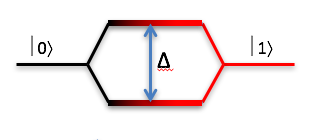
\includegraphics[height=4cm]{newSystem}
	   	\caption{\small The original states have the same energy, but the superposition ones are split. \label{fig:newSystem}}
   	\end{center}
   \end{figure}
   
   \textbf{Now we add an electric field} to the quantum wells, see Fig.\ref{fig:withField}. The energy shift from the field is $e\vec{E}\vec{d}$, where $\vec{d}$ is the distance between the two wells. We have a two level system, and we define the zero energy to be halfway between them, making the Hamiltonian
   
   \begin{equation}
   \label{l1-1}
   \mathcal{H}_{\text{no tunneling}} = -\frac{\epsilon}{2}\sigma_z = \left(\begin{matrix}
   -\epsilon/2 & 0\\ 0 & \epsilon/2
   \end{matrix}\right).
   \end{equation}
   
   \begin{figure}
   	\begin{center}
   		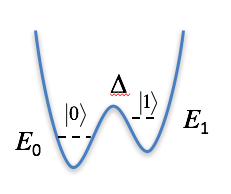
\includegraphics[height=3cm]{withField}
   		\caption{\small Adding an electric field, will mean that one well state is at a higher energy (higher potential energy).}
   		\label{fig:withField}
   	\end{center}
   \end{figure}

   \textbf{Now tunnelling + electric field gives us }
   
   \begin{equation}
	   \label{l1-newH}
	   \begin{aligned}
	   \mathcal{H} = \left(\begin{matrix}
	   -\epsilon/2 & 0\\ 0 & \epsilon/2
	   \end{matrix}\right) + \begin{pmatrix}
	   0 & -\Delta/2\\-\Delta/2 & 0
	   \end{pmatrix} & = {-\frac{\epsilon}{2}\sigma_z-\frac{\Delta}{2}\sigma_x}\\
	   & = -\frac{\sqrt{\epsilon^2+\Delta^2}}{2}\left(\frac{\epsilon}{\sqrt{\epsilon^2+\Delta^2}}\sigma_z+\frac{\Delta}{\sqrt{\epsilon^2+\Delta^2}}\sigma_x\right)\\
	   & = -\frac{\Delta E}{2}\left(\cos\left(\theta\right)\sigma_z+\sin\left(\theta\right)\sigma_x\right)\\
	   \red{\Rightarrow \left\lbrace\begin{aligned}
	    \mathcal{H} & = \mathbf{-\frac{\Delta E}{2}\begin{pmatrix}
	   		\cos(\theta) & \sin(\theta)\\\sin(\theta) & -\cos(\theta)
	   		\end{pmatrix}}\\
   		\Delta E & = \sqrt{\epsilon^2+\Delta^2}\\
   		\tan(\theta) & = \frac{\Delta}{\epsilon}
	   \end{aligned}\right.} 
	   \end{aligned},
   \end{equation}
   
   \noindent \red{\text{ small $\theta$ = small mixing.}}. Finding eigenvalues and eigenvectors 
   
   \begin{equation}
	   E = \pm \frac{\Delta E}{2}, \qquad \ket{\psi}_0 = \begin{pmatrix}
	    \cos(\theta/2) \\ \sin(\theta/2)
	   \end{pmatrix}, \qquad \ket{\psi}_1 = \begin{pmatrix}
		    \sin(\theta/2) \\ -\cos(\theta/2)
	   \end{pmatrix},
	   \label{l1-finalEVal}
   \end{equation}

   \noindent and we note that inside the Bloch Sphere, the eigenstates are now at an angle $\theta$ relative to the initial ``north-south'' eigenstates as seen in Fig.\ref{newEigenstates}
   
   \begin{figure}[h]
   	\begin{center}
   		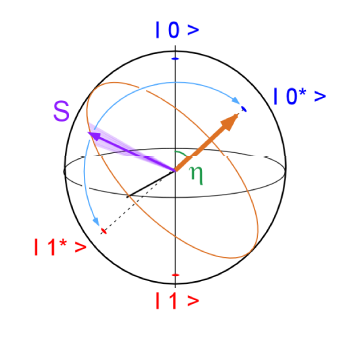
\includegraphics[height=4.5cm]{newEigenstates}
   		\caption{\small The drive $\Delta$, tilts the eigenstates of the system. \red{$\tan(\theta) = \frac{\Delta}{\epsilon}$}}
   		\label{newEigenstates}
   	\end{center}
   \end{figure}
   
   \iframe{\noindent So we have gone from a purely potential system with $\mathcal{H} = -\epsilon/2\sigma_z$, and a purely kinetic system with $\mathcal{H} = -\Delta/2\sigma_x$, to a mixed one as shown in Fig.\ref{l1-combined}.}
   
   \begin{figure}[h]
   	\begin{center}
   		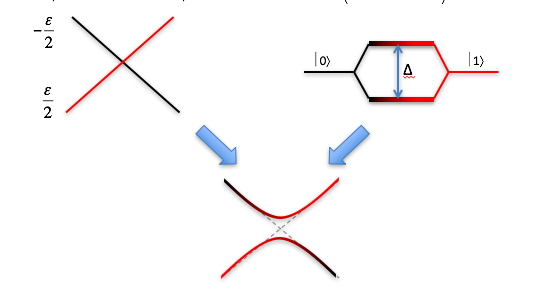
\includegraphics[height=7cm]{together}
   		\caption{\small In the potential system, the energies of the eigenstates changed linearly with field. At the crossing point (no field), there is a degeneracy, where both wells are at the same potential. The kinetic tunnelling case we have also seen. Together they form a system whose eigenstates are split.}
   		\label{l1-combined}
   	\end{center}
   \end{figure}
 

   	\textbf{Considering the case with no bias $\mathbf{\epsilon = 0 \Rightarrow \Delta E = \Delta, \theta = \pi/2}$:}
   	
   	\[
   	 \mathcal{H} = -\frac{\Delta}{2}
   	 \begin{pmatrix}
   		0 & 1\\ 1 & 0
   	 \end{pmatrix} = -\frac{\Delta}{2} \sigma_x.
   	\]
 
   \noindent Computing the unitary evolution of the state
   
   \begin{equation}
	   \begin{aligned}
		   U & = \exp\left[\frac{-i\mathcal{H}t}{\hbar}\right]\\
		   & = \sum_k\frac{-i\Delta/2\sigma_xt}{k!}\\
		   & \red{=
			   \cos\left(\frac{\Delta}{2\hbar}t\right)\mathbb{I} + i\sin\left(\frac{\Delta}{2\hbar}t\right)\sigma_x = \begin{pmatrix}
				   \cos\left(\frac{\Delta}{2\hbar}t\right) & i\sin\left(\frac{\Delta}{2\hbar}t\right)\\
				   i\sin\left(\frac{\Delta}{2\hbar}t\right) & \cos\left(\frac{\Delta}{2\hbar}t\right)
			   \end{pmatrix}}
	   \end{aligned},
	   \label{l1-finalRot}
   \end{equation}
   
   \noindent so 
   
   \begin{equation}
	   U\ket{0} = \begin{pmatrix}
		   \cos\left(\frac{\Delta}{2\hbar}t\right)\\
		   i\sin\left(\frac{\Delta}{2\hbar}t\right),
	   \end{pmatrix},
   \end{equation}
   
   \noindent so we can prepare any state perpendicular to the x-axis.
   
  \iframe{Thus no bias + tunneling $ \equiv $ bias + resonant field in RWA. In both cases, the interaction causes the same state evolution}
   
  \newpage 
%
% -*- TeX-master: "../all_the_notes.tex" -*-

\section{Quantum Electrodynamics Formalism\label{subsec:l2-CPB}}

   \subsection{Superconductors}
   In superconductors CP carry charge.   What happens is that the Fermi
   level  splits into  2 bands  that  are $\pm\Delta$  above and  below
   $E_F$, and each electron in the CP belongs to one of these bands.


   {{ Phase is quantised in a sc loop
       \begin{equation}
         \begin{aligned}
           \phi = \phi_\text{ext} + 2\pi N  \Leftrightarrow \Phi = \Phi_\text{ext} + \Phi_0
           \\(\Phi_0 = \frac{h}{2e}, \Phi/\Phi_0=\phi/2\pi)
         \end{aligned}
       \end{equation}
     }}

   \subsection{Josephson junction}
   Now  work with  JJ.  The  states  on the  two  sides of  the JJ  are
   $\left|\psi_0\right|e^{i\phi_1}$                                 and
   $\left|\psi_0\right|e^{i\phi_2}$.  Solving  the Schrodinger equation
   for the condensate state, when E=0

   \begin{equation}
     -\frac{\hbar^2}{2m}\iderivative{^2}{x^2}\psi+U\psi = 0 \Rightarrow
     \left\lbrace\begin{aligned}
         \psi & = A_0e^{-kx}+B_0e^{+kx}\\
         k & = \frac{\sqrt{2mU}}{\hbar}
       \end{aligned} \right. \Rightarrow \left\lbrace\begin{aligned}
         \psi & = A\cosh(kx)+B\sinh(kx)\\
         k & = \frac{\sqrt{2mU}}{\hbar}
       \end{aligned} \right.
   \end{equation}

   \noindent            Apply            BC           for            JJ
   $\psi(a/2)        =       \left|\psi_0\right|e^{i\phi_2}$        and
   $\psi(-a/2) = \left|\psi_0\right|e^{i\phi_1}$ to find that

   \begin{align}
     A &= \frac{\left|\psi_0\right|}{\cosh(ka/2)}\\
     B &= \frac{\left|\psi_0\right|}{\sinh(ka/2)}.
   \end{align}

   \noindent {The super current is then}

   \begin{equation}
     I = -\frac{i\hbar}{2m}(2e)\left[\psi^*\iderivative{\psi}{t}-\psi\iderivative{\psi^*}{t}\right] \equiv -\frac{2e\hbar}{m}\text{Im}\left[\psi^*\iderivative{\psi}{t}\right],
   \end{equation}

   \noindent at $x=0$ can be evaluated,  as can the voltage and energy,
   which results in a phase dependence

   \begin{equation}
     \label{l2-dcac}
     I = I_c\sin(\phi_2-\phi_1); \qquad \frac{d\phi}{dt} = \frac{2e}{\hbar}V
   \end{equation}

   The phase  across the JJ  in a circuit is  the phase induced  by the
   external flux i.e.

   \begin{equation}
     \label{eqn:l2-phasesum}
     \phi_1+\phi_2+\ldots = \phi_\text{ext} = \frac{\Phi_\text{ext}}{\Phi_0}2\pi,
   \end{equation}

   \begin{equation}
     \left\lbrace\begin{aligned}
         I &= I_c\sin(\phi_2-\phi_1)\equiv I_c\sin(\phi)\\
         V&=\dot{\Phi} \equiv \frac{\dot{\phi}}{2\pi}\Phi_0
       \end{aligned}\right. \Rightarrow U = \left\lbrace\begin{aligned}
         \int_{0}^{t}IV dt & = \int_{0}^{t}I_c\sin(\phi)\frac{\Phi_0}{2\pi}\frac{d\phi}{dt}dt\\
         & = \int_{0}^{\phi} E_J\sin(\phi)d\phi\\
         & \red{= E_J(1-\cos(\phi)),\qquad E_J = \frac{\Phi_0I_c}{2\pi}.}
       \end{aligned}\right.
     \label{l2-JJEnergy}
   \end{equation}

  \begin{center}
    Increase $  I $ \ira Increase  $ \phi =  \phi_2-\phi_1 $ to $  \pi/2 $
    \ira Increse  energy $  U $  \ira \textbf{at  some point,  we reach
      critical currrent and highest energy - beyond this limit, we will
      generate voltage}


\begin{figure}[h]
  \centering 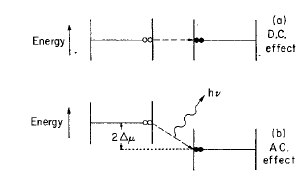
\includegraphics[height=3cm]{josephson_effecti}
\end{figure}

\noindent
\end{center}

\paragraph{Inductance} is found by performing:

\begin{itemize}
\item Suppose  a change  in current,  $ \delta_I $  causes a  change in
  phase $ \delta_1\phi $:

    \begin{equation}\label{key}
      I_0 + \delta_I = I_c\sin(\phi_0+\delta_\phi) \iRa \delta_I = \purple{I_c\cos(\phi_0)\delta_\phi.}
    \end{equation}
  \item The voltage across the junction:
    \begin{equation}\label{key}
      V = \frac{\dot{\phi}}{2\pi}\Phi_0 = \frac{\Phi_0}{2\pi}\left(\red{\dot{\phi}_0} + \dot{\delta}_\phi\right) =  \frac{\Phi_0}{2\pi}\purple{\frac{\dot{\delta}_I}{I_c\cos(\phi_0)}}.
    \end{equation}

  \item FInally expressing the inductance

    \begin{equation}\label{key}
      L = V/\frac{dI}{dt} = V/\dot{\delta}_I = \frac{\Phi_0}{2\pi}\frac{1}{I_c\cos(\phi_0)}.
    \end{equation}
  \end{itemize}

  \begin{framed}\noindent
    \begin{equation}\label{key} L_J = \Phi/I =
      \frac{\Phi_0}{2\pi}\frac{1}{I_c}\frac{1}{\cos(\phi_0)}
    \end{equation}
  \end{framed}

  \noindent The current is given by:

   \begin{equation}\label{key}
     I_cR_n = \frac{\pi\Delta(T)}{2e}\tanh\big(\frac{\Delta(T)}{2k_bT}\big),
   \end{equation}

   \noindent derived from  BCS theory for a  superconducting energy gap
   of $ \Delta(T) $ and normal resistance $ R_n $ of the JJ.

   {
     \paragraph{Critical current $ I_c $}
     Taking the limit of $ T\ira0 $ we get

    \begin{equation}\label{app:criticalCurrent}
      I_cR_n = \frac{\pi\Delta(0)}{2e}
    \end{equation}
  }


  \begin{framed}\noindent
    \paragraph{Josephson   Energy  from   JJ  parameters}   Subbing  in
    Eq.~\eqref{app:criticalCurrent} into Eq.~\eqref{l2-JJEnergy}:

    \begin{equation}\label{key}
      \begin{aligned}
        E_J & = \frac{R_q}{R_n/N_{sq}}\frac{\Delta(0)}{2}\\
        R_n &= 18.4\,\text{k}\Omega \text{ for 100 } \times 100\,\text{nm}^2
      \end{aligned}
    \end{equation}

    \noindent with $  R_q = \frac{h}{(2e)^2} $. The wider  the JJ is in
    squares, $ N_{sq} $, the lower the resistance of the junction.

    \red{JJ resistance increases by $ \sim 10\% $ as one goes from room to
      cryogenic temperatures.}
  \end{framed}

   \subsubsection{Inductance energy}
   Inductance              energy             derives              from
   $                        \frac{\Phi_L^2}{2L}                       =
   \frac{\Phi_0^2}{(2\pi)^22L}(\phi_\text{ext}-\phi_J)^2              =
   E_L(\phi_\text{ext}-\phi_J)^2 $

   \begin{equation}
     \begin{aligned}
       E_L & = \frac{\Phi_0^2}{(2\pi)^22L}\\
       L & \propto R_n = \iunit{1.5}{nH per 100}\times\iunit{100}{nm}^2
     \end{aligned}
   \end{equation}

   \subsubsection{Summary of energies}
   \begin{table}[h]
     \centering {%
       \footnotesize%
       \begin{tabular}{|c|c|p{6cm}|c|}%
         \hline\textbf{Energy}    &    &    \textbf{Variable   parameter}    &    \textbf{Energy
                                                                               ($  N_{sq}=10,  N_{NbN} =  5$)}
         \\\hline
         $ E_J $ & $ \frac{R_q}{R_{\square}/N_{sq}}\frac{\Delta(0)}{2} $ & $ R_q = \frac{h}{(2e)^2} = 6.484\,\text{k}\Omega,\newline \Delta = 1.73*(k_b\times 1.3\,\text{K}) = 3.1\times10^{-23}, \newline R_\square = \iunit{18.4}{k}\Omega $ & \iunit{77.5}{GHz} \\
         $ E_C $ & $ \frac{(2e)^2}{2CN_{sq}} $ & $ \varepsilon = 10, d = \iunit{2}{nm}, \newline A = 100\times\iunit{100}{nm}^2, \newline C = \frac{\varepsilon\varepsilon_0A}{d} = \iunit{0.5}{fF} $ & \iunit{17.4}{GHz} \\
         $      E_L       $      &      $      \frac{\Phi_0^2}{(2\pi)^22LN_{NbN}}       $      &
                                                                                                 $\Phi_0
                                                                                                 =2\times{-15}\,\text{Wb},\newline
                                                                                                 L
                                                                                                 =
                                                                                                 \iunit{1.5}{nH}
                                                                                                 $
                                                                                                 per
                                                                                                 NbN
                                                                                                 square
                                                                             &
                                                                               \iunit{16.2}{GHz}\\\hline
       \end{tabular}
     }
   \end{table}

   \subsection{SQUID to control $ E_J $\cite{zhu2010}}
   \begin{framed}\noindent
     Inductance of a SQUID:
     \begin{equation}\label{l2:squid:inductance}
       L_J(\Phi_\text{ext}) = V/\frac{dI}{dt} = \frac{\hbar}{4eI_c|\cos(\pi\Phi_\text{ext}/\Phi_0)}.
     \end{equation}
   \end{framed}

   Two JJ in a loop give a total current

    \begin{equation}
      I = I_{c1}\sin(\phi_1)+I_{c2}\sin(\phi_2),
    \end{equation}

    \noindent  which  along  with   the  phase  quantisation  condition
    Eq.\eqref{eqn:l2-phasesum}  and  symmetric JJs  $I_{c1}=I_{c2}=I_c$
    results in

    \begin{equation}
      \begin{aligned}
        I = & I_{cs}(\Phi_\text{ext})\sin(\phi)\\
        & I_{cs} = 2I_c|\cos(\pi\Phi_\text{ext}/\Phi_0)|\\
        & \phi = (\phi_1+\phi_2)/2
      \end{aligned},
    \end{equation}

    \noindent which has  a similar form to  Eq.\eqref{l2-dcac}, but now
    the  critical  current  $I_{cs}$   is  controlled  by  an  external
    field. Taking the derivative

    \begin{equation}
      \begin{aligned}
        \frac{dI}{dt}=2I_{cs}(\Phi_\text{ext})\cos(\phi)\frac{d\phi}{dt},
      \end{aligned}
    \end{equation}

    \noindent and  expressing the voltage using  Eq.\eqref{l2-dcac} and
    assuming $\cos(\phi)\approx1$ for small excitations

    \begin{equation}
      V = \frac{\hbar}{2e}/\frac{d\phi}{dt} = \frac{\hbar}{4eI_{cs}}\frac{dI}{dt},
    \end{equation}

    \noindent     from    which     one     finds    the     inductance
    ($\Phi = LI \rightarrow L = \frac{d\Phi}{dI} = \frac{d\Phi}{dt}/\frac{dI}{dt}
    = V/\frac{dI}{dt}$for small excitations

    \begin{equation}
      L_J(\Phi_\text{ext}) = V/\frac{dI}{dt} = \frac{\hbar}{4eI_c|\cos(\pi\Phi_\text{ext}/\Phi_0)}.
    \end{equation}
    \vspace{6ex}

   \subsection{Building blocks for quantum circuits.}
   Quantum circuits are built from
   \begin{itemize}
   \item    JJs,   who    posses    an    inductance   $L_J$    defined
     Eq.\eqref{l2:squid:inductance}.   The energy  comes from  the flux
     stored by the inductor
     \begin{equation}
       E_J(\Phi_\text{ext}) = \frac{\Phi_0}{2L_J(\Phi_\text{ext})}
     \end{equation}
   \item  An inductor  $L$  with  energy from  a  the  flux inside  the
     inductor (coil)
     \begin{equation}
       E_L = \frac{\Phi^2}{2L}
     \end{equation}
   \item A capacitor with energy
     \begin{equation}
       E_c = \frac{Q^2}{2C}
     \end{equation}
   \end{itemize}

   For the most general discussion, we compare

   \setlength{\extrarowheight}{4mm}
   \begin{table}[h]
     \caption{}
     \label{tab:conversion1}
     \begin{center}
       \begin{tabular}{|c|c|c|c|}
         \hline
         &\textbf{$ Q $ and $ \Phi $} & \textbf{Mechanical} & \textbf{$ V $ and $ I $} \\\hline
         \multicolumn{4}{|c|}{$ I =\dot{Q }\qquad V=\dot{\Phi} $}\\
         \multicolumn{4}{|c|}{$ Q=CV\qquad \Phi = LI $}\\\hline
         \multirow{2}{*}{Kinetic} & $ \frac{Q^2}{2C} $  & $ \frac{p^2}{2m} $ & \textit{\scriptsize Inductor}\\
         & \textit{\scriptsize Capacitor} & $ \frac{m\dot{x}^2}{2} $& $ \frac{LI^2}{2} = \frac{LC^2\dot{V}^2}{2}$ \\\hline
         Potential & $ \frac{\Phi^2}{2L} $ & $ \frac{kx^2}{2} $ & $\frac{CV^2}{2}$ \\
         & \textit{\scriptsize Inductor} & & \textit{\scriptsize Capacitor} \\\hline
         $ \omega_0 $ & $  \frac{1}{\sqrt{LC}} $ &$  \sqrt{\frac{k}{m}} $ &$  \frac{1}{\sqrt{LC}} $\\\hline
         \multirow{2}{*}{Energy} & $\frac{Q^2}{2C}+\frac{1}{2}C\omega_0^2\Phi^2$ & $\frac{p_m^2}{2m}+\frac{1}{2}m\omega_m^2x^2$ & \\
         & & $\frac{m}{2}\left(\dot{x}^2+\omega_0^2x^2\right)$  & $ \frac{LC^2}{2}\left(\dot{V}^2+\omega_0V^2 \right)$\\\hline
         Momentum & $ Q $ & $ p $ & $I =  C\dot{V} $\\\hline
         Coordinate & $ \Phi $ & x & V\\\hline
         Mass & $ C $ & $ m $ & $ LC^2 $\\\hline
         Stiffness & $ \frac{1}{L} $ & $ k $ & C\\\hline
         Solution &$ \Phi=Ae^{i\omega_0t}+Be^{-i\omega_0t} $ & $ x=Ae^{i\omega_0t}+Be^{-i\omega_0t} $ & $ V=Ae^{i\omega_0t}+Be^{-i\omega_0t} $\\\hline
       \end{tabular}
     \end{center}
   \end{table}

   \setlength{\extrarowheight}{4mm}
   \begin{table}[h]
     \caption{}
     \label{tab:conversion2}
     \begin{center}
       \begin{tabular}{|c|c|c|c|}
         \hline
         &\textbf{$ Q $ and $ \Phi $} & \textbf{Mechanical} & \textbf{$ V $ and $ I $} \\\hline
         Momentum & $ Q $ & $ p $ & $I =  C\dot{V} $\\\hline
         Coordinate & $ \Phi $ & x & V\\\hline
         Mass & $ C $ & $ m $ & $ LC^2 $\\\hline
         Stiffness & $ \frac{1}{L} $ & $ k $ & C\\\hline
         \multirow{2}{*}{Energy} & $\frac{Q^2}{2C}+\frac{1}{2}C\omega_0^2\Phi^2$ & $\frac{p_m^2}{2m}+\frac{1}{2}m\omega_m^2x^2$ & \\
         & & $\frac{m}{2}\left(\dot{x}^2+\omega_0^2x^2\right)$  & $ \frac{LC^2}{2}\left(\dot{V}^2+\omega_0V^2 \right)$\\\hline
         \multirow{3}{*}{$ \mathcal{H} $} & \multirow{2}{*}{$ \frac{\hbar\omega_0}{2}\left(\frac{Q^2}{Q_0^2}+\frac{\Phi^2}{\Phi_0^2}\right) $} &  \multirow{2}{*}{$ \frac{\hbar\omega_0}{2}\left(\frac{\hat{p}^2}{p_0^2}+\frac{\hat{x}^2}{x_0^2}\right) $} & \multirow{2}{*}{$ \frac{\hbar\omega_0}{2}\left(\frac{\hat{I}^2}{I_0^2}+\frac{\hat{V}^2}{V_0^2}\right) $}\\
         & & & \\
         & $ \Phi_0=\sqrt{\frac{\hbar\omega_0}{C}},\  Q_0 = \sqrt{\frac{\hbar}{C\omega_0}} $& $ x_0 = \sqrt{\frac{\hbar}{m\omega_0}},\ p_0 = \frac{\hbar}{x_0} $ & $ V_0 = \sqrt{\frac{\hbar\omega_0}{C}},\ I_0 = \sqrt{\frac{\hbar\omega_0}{L}} $ \\\hline
         & \parbox[c]{5cm}{$ \left[\hat{\Phi},\hat{Q}\right] = i\hbar $ since $ \Phi $ and $ Q $ are exactly $ x $ and $ p $}& $ \left[\hat{x},\hat{p}\right] = i\hbar $ & \parbox{5cm}{$ \left[\hat{\Phi},\hat{Q}\right] = \left[CV,LI\right]=i\hbar $ so $ \left[\hat{V},\hat{I}\right] = \frac{i\hbar}{LC}$}\\\hline
         & $ \hat{\Phi} $& $ \hat{x} $ & $ \hat{V} $\\\hline
         & $ \hat{Q}=-i\hbar\frac{d}{d\Phi} $& $ \hat{p} = -i\hbar\frac{d}{dx} $ & $ \hat{I} = -i\frac{\hbar}{LC}\frac{d}{dV} $\\\hline
         & \multirow{2}{*}{$ a^{\dagger} = \sqrt{\frac{C\omega_0}{2\hbar}}\left(\hat{\Phi}-i\frac{\hat{Q}}{C\omega_0}\right) $} & \multirow{2}{*}{$ a^{\dagger} = {\frac{1}{\sqrt{2}}}\left(\frac{\hat{x}}{x_0}-i\frac{\hat{p}}{p_0}\right) $} & \multirow{2}{*}{$ a^{\dagger} = {\frac{1}{\sqrt{2}}}\left(\frac{\hat{V}}{V_0}-i\frac{\hat{I}}{I_0}\right) $}\\
         & & & \\\hline
       \end{tabular}
     \end{center}
   \end{table}

   We  see  that  in  either  case, we  are  working  with  a  harmonic
   oscillator   system,  with   corresponding   raising  and   lowering
   operators.

   {\scriptsize As a reminder, an equation with the form
     \[
       \mathcal{H}                                                    =
       \frac{\hbar\omega_0}{2}\left(y^2-\frac{^2}{y^2}\right)
     \]

     \noindent can be rewritten as

    \[
      \mathcal{H}    =    \hbar\omega_0\left(a^{\dagger}a+\frac{1}{2}\right)=
      \hbar\omega_0\left(\hat{N}+\frac{1}{2}\right)
    \]

    with eigenstates and eigenenenergies

    \[
      \ket{\Psi}_n=\ket{n} \qquad E_n= \hbar\omega_0\left(n+\frac{1}{2}\right).
    \]

    \noindent The raising  and lowering operators act  in the following
    way on the eigenstates

    \[
      \left\lbrace\begin{aligned}
          a\ket{n} & = \sqrt{n}\ket{n-1}\\
          a^{\dagger}\ket{n} &= \sqrt{n+1}\ket{n+1}\\
        \end{aligned}\right. \Rightarrow
      \hat{N}\ket{n}       =       a^{\dagger}      \sqrt{n}\ket{n-1}       =
      \sqrt{n}^2\ket{n}=n\ket{n} ,
    \]
    \noindent  and the  matrix form,  evaluated by  finding the  matrix
    coefficients $ c_{ij}=\bra{i}\hat{C}\ket{j} $

    \[
      \hat{a}=\begin{pmatrix}
        0 & \sqrt{1} & 0 & 0\\
        0 & 0 & \sqrt{2} & 0\\
        0 & 0 & 0 & \sqrt{3}\\
        0 & 0 & 0 & \ddots\\
      \end{pmatrix} \qquad a^{\dagger}=\begin{pmatrix}
        0 & 0 & 0 & 0\\
        \sqrt{0+1} & 0 & 0 & 0\\
        0 & \sqrt{1+1} & 0 & 0\\
        0 & 0 & \sqrt{2+1} & \ddots\\
      \end{pmatrix} \qquad \hat{N} =\begin{pmatrix}
        0 & 0 & 0 & 0\\
        0 & 1 & 0 & 0\\
        0 & 0 & 2 & 0\\
        0 & 0 & 0 & \ddots\\
      \end{pmatrix}
    \]
  }

  For the Harmonic  oscillator which the system  replicates, the energy
  levels are evenly spaced, making  it impossible to address individual
  states.  But by replacing the inductor with a JJ

   \begin{equation}
     E_L = \frac{\Phi^2}{2L} \longrightarrow U = -E_J\cos(\phi),
   \end{equation}

   \noindent changing the quadratic to a cosine potential.
   \newpage
%
\section{Charge basis\label{sec:charge_basis}}
 \red{\textbf{The charge basis is used, when the energy is mostly capacitive.}}
 
 \begin{itemize}
 	\item \red{It is not continous wavefunctions}, but raising and lowering operators and discreete charge states \iket{0}, \iket{1}, \iket{2}, \iket{3} \ldots;
 	\item The operators are defined as
 	\begin{equation}\label{key}
 		\hat{\red{N}}\ket{n} = n\iket{n}\qquad\qquad e^{\pm i\blue{\phi}} = \sum_n\ketbra{n\pm 1}{n} \qquad\qquad \left[\blue{\phi},\red{N}\right] = \frac{2\pi}{\frac{h}{2e}}\left[\Phi,Q\right]\frac{1}{2e} = i
	\end{equation}
 
 \noindent $ n $, is the number of Cooper pairs that have tunneled to an island via the Josephson junction.
 \end{itemize}

\subsection{Proovind the phase raising effect}
 Let us understand, where the phase operator definition
 \begin{equation}\label{key}
 	e^{\pm i\blue{\phi}} = \sum_n\ketbra{n\pm 1}{n},
 \end{equation}
 
 \noindent is coming from. 
 
 \begin{enumerate}
 	\item Looking at the commutation relation
 
 \begin{equation}\label{key}
 	\begin{aligned}
	 	\icommutation{\hat{\red{N}}}{e^{\pm i \hat{\blue{\phi}}}} = &  \icommutation{\hat{N}}{\sum_{\alpha = 0}^{\infty} \frac{(\pm i\hat{\blue{\phi}})^\alpha}{\alpha!}}\\
	 	& = \sum_{\alpha = 0}^{\infty} (\pm i)^\alpha\frac{\icommutation{\hat{\red{N}}}{\hat{\blue{\phi}}^\alpha}}{\alpha!} \qquad \icommutation{\hat{\red{N}}}{\hat{\blue{\phi}}} = -i, \icommutation{A}{BC} = B\icommutation{A}{C} + \icommutation{A}{B}C
	 	\\
	 	& = \sum_{\alpha = 0}^{\infty} (\pm i)^\alpha\frac{-\alpha i\hat{\blue{\phi}}^{\alpha - 1}}{\alpha!}\\
	 	& = \pm \sum_{\alpha = 1}^{\infty}i^{\alpha - 1}\frac{(\pm\hat{\blue{\phi}})^{\alpha - 1}}{(\alpha - 1)!}\\
	 	& = \pm e^{\pm i\hat{\blue{\phi}}}
 	\end{aligned}
 \end{equation}
 \item Next, if we evaluate
 \begin{equation}\label{key}
 	\begin{aligned}
 	\hat{\red{N}}\bigg[e^{\pm i\hat{\blue{\phi}}}\ket{n}\bigg] & = \bigg[\pm e^{\pm i\hat{\blue{\phi}}} + e^{\pm i\hat{\blue{\phi}}}\hat{N}\bigg]\ket{n}\\
 	& = (n\pm 1)\bigg[e^{\pm i\hat{\blue{\phi}}}\ket{n}\bigg]
 	\end{aligned}
 \end{equation}
 \item  So in effect, what we can say is that the action of the phase operator increments the $ n $ number like a ladder operator:
 
 \begin{equation}\label{key}
 	\begin{aligned}
 	e^{\pm i\hat{\blue{\phi}}}\ket{n} &= C\ket{n \pm 1}\qquad \text{(since $ e^{\pm i\hat{\blue{\phi}}} $ is unitary)}\\
 	&= \ket{n\pm 1}
 	\end{aligned}
 \end{equation}
 \item \ 
 \iframe{So therefore, we can write the phase operator in the following form
 	\begin{equation}\label{key}
 		\begin{aligned}
	 		e^{\pm i\hat{\blue{\phi}}} & = \sum_{n}\ketbra{n\pm 1}{n}\\
	 		\hat{\red{N}} & = \sum_{n}n\ketbra{n}{n}.
 		\end{aligned}  
 	\end{equation}
 }
 \end{enumerate}
 
\newpage 
%
\section{Phase basis}
 \red{\textbf{The phase basis is used, when the energy is mostly from the JJ, such as an RF-SQUID}}
 
 \begin{itemize}
 	\item We work with wavefunction $ \psi(\phi) $ in phase-space;
 	\item For the operators we take
 	\begin{equation}\label{key}
 		\blue{\hat{\phi}} \qquad \qquad \red{\hat{N}} = -i\frac{d}{d\blue{\phi}}\qquad\qquad \left[\blue{\phi},\red{N}\right] = \frac{2\pi}{\frac{h}{2e}}\left[\Phi,Q\right]\frac{1}{2e} = i\\
 	\end{equation}
 \end{itemize}

 The Cooper pair box Hamiltonian will read
 \begin{equation}\label{key}
 	\mathcal{H} = E_c\left(-i\frac{d}{d\phi} - n_g\right)^2 - E_J\cos(\phi).
 \end{equation}
\newpage %
\newpage

\section{Two Level System}
\label{sec:two-level-system}

\begin{framed}\noindent
  \begin{itemize}
  \item Cause dissipation and decoherence in qubits with JJ.
  \item  Can be  an  electron or  ion with  two  potential wells  and
    tunneling between them.
  \item  Phase difference  across the  junction will  couple via  the
    electric field across the junction:
    \begin{equation}
      \mathcal{\varepsilon} = \frac{\dot{\varphi}}{d},
    \end{equation}

    \noindent where $d$ is the thickness of the JJ.
  \item  Activated when  the frequency  across the  JJ matches  their
    energy separation:
    \begin{equation}
      \hbar\omega_{J}
    \end{equation}

    \noindent and after  which Rabi oscillations can  occur. The rate
    of rabi oscillation  ($\Omega_R$) depends on the  strength of the
    coupling.
  \end{itemize}
\end{framed}

\begin{figure}[h]
  \centering
  \includegraphics[height=7cm]{2005_martin_tunneling-spectroscopy-of-two-level-systems-inside-a-josephson-junction/fig1}
  \caption{\small
    Setup\label{fig:2005_martin_tunneling-spectroscopy-of-two-level-systems-inside-a-josephson-junction/fig1}}
\end{figure}



%%% Local Variables:
%%% mode: latex
%%% TeX-master: "all_the_notes"
%%% End:
%

%% Specific systems
\section{Single cooper pair box system\label{sec:cooper_pair_box}}
The Cooper pairs are trapped on an island between a gated capacitor and a Josephson junction.
\begin{figure}[h]
  \centering 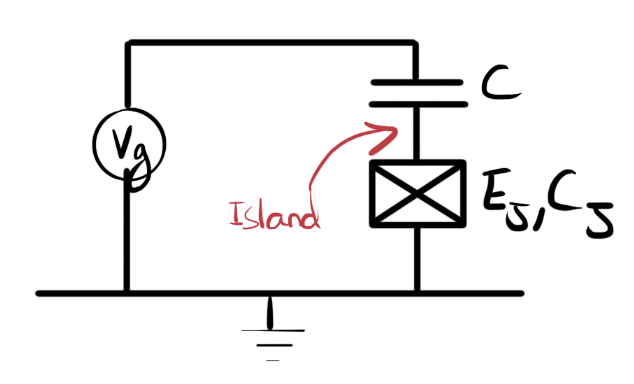
\includegraphics[height=4cm]{cooper_pair_box}
\end{figure}

\noindent

\begin{framed}\noindent
  We remember that the voltage induction law reads
  \begin{equation}\label{key}
    V = -\dot{\Phi}.
  \end{equation}
\end{framed}


\begin{enumerate}
\item Forgetting about  the voltage source, we consider  the following diagram, which will  have a \red{\textbf{charging
      kinetic part}}

  \begin{equation}\label{key}
    T = \frac{C_g}{2}\dot{\Phi_J}^2 + \frac{C_J}{2}\dot{\Phi_J}^2 = \frac{C_\Sigma}{2}\dot{\Phi_J}^2.
  \end{equation}

\begin{figure}[h]
  \centering 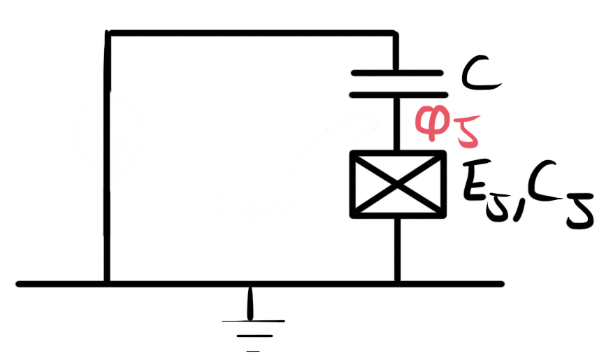
\includegraphics[height=3cm]{cooper_pair_box_1}
\end{figure}

\noindent

\item \textbf{\red{The potential  energy part}} comes from the JJs  and the energy supplied by the  source acting on the
  gate side of the gate capacitor (note that we are free to choose the sign of the biasing voltage.
  \begin{equation}\label{key}
    \begin{aligned}
      & E_J = 1 - E_J\cos(\frac{2\pi}{\Phi_0}\Phi_J)\\
      & \begin{aligned}
        E_\text{gate} & = V_g \times Q_c\\
        Q_c & = C_g\times -\dot{\Phi_J}
      \end{aligned}
    \end{aligned}\ira U = -E_J\cos(\frac{2\pi}{\Phi_0}\Phi_J) - V_gC_g\dot{\Phi_J}.
  \end{equation}

\begin{figure}[h]
  \centering 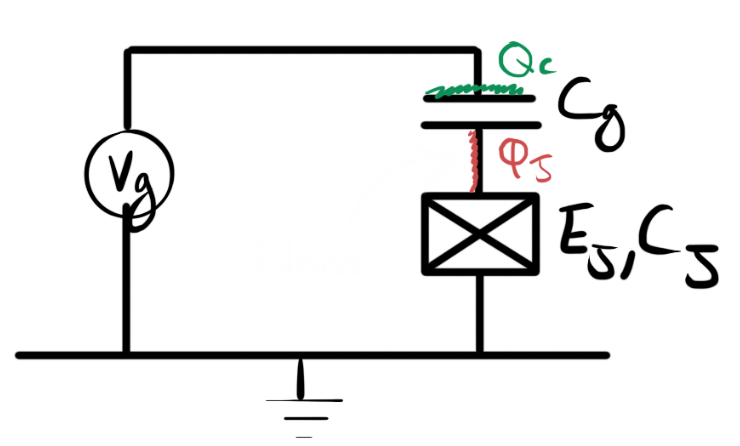
\includegraphics[height=3cm]{cooper_pair_box_2}
\end{figure}

\noindent

\item The full \red{\textbf{Lagrangian}} now reads
  \begin{equation}\label{key}
    \mathcal{L} = T - U = \frac{C_\Sigma}{2}\dot{\Phi}_J^2 + E_J\cos(\frac{2\pi}{\Phi_0}\Phi_J) + V_gC_g\dot{\Phi_J}.
  \end{equation}

\item The \textbf{\red{conjugate momentum}}
  \begin{equation}\label{key}
    Q_J = \frac{d\mathcal{L}}{d\dot{\Phi}_J} = C_\Sigma\dot{\Phi}_J + V_gC_g,
  \end{equation}
  \noindent is just an offset of the induced charge on the capacitor due to the JJ voltage with the gate induced charge.

\item So we arrive at the following set of variables

  \begin{equation}
    { \textcolor{blue}{\mathbf{x\leftrightarrow \Phi \leftrightarrow \phi} \text{ (position/flux) }}\qquad \textcolor{red}{\mathbf{p\leftrightarrow Q \leftrightarrow N \text{ (momentum/electrons) }}}}
  \end{equation}

  \noindent with the commutation relations:

  \begin{align}
    \left[\blue{x},\red{p}\right] & =i\hbar & \left[\blue{\Phi},\red{Q}\right] & = i\hbar & \left[\phi,N\right] & = \frac{2\pi}{\frac{h}{2e}}\left[\Phi,Q\right]\frac{1}{2e} = i\\
    \red{\hat{p}} & = -i\hbar\ipartial{}{\blue{x}} & \hat{\red{Q}} & =-i\hbar\ipartial{}{\blue{\Phi}} & \hat{\red{N}} & =-i\ipartial{}{\blue{\phi}}
  \end{align}

\item\

\begin{framed}\noindent
  Expressing the \red{\textbf{Hamiltonian}} in the standard fashion

  \begin{equation}\label{eqn:cpbox_final}
    \begin{aligned}
      \mathcal{H} & = Q_J\dot{\Phi}_J - \mathcal{L}\\
      & = \frac{(Q_J - C_gV_g)^2}{2C_\Sigma} - E_J\cos(\frac{2\pi}{\Phi_0}\Phi_J)\\
      &     =      \mathbf{\red{E_C{\left(\hat{N}-N_\text{ext}\right)^2}-     E_J\cos\left(\phi\right)}}\qquad      E_c     =
      \frac{(2e)^2}{2C_\Sigma}
    \end{aligned}
  \end{equation}

  \noindent Wel call $ N_\text{ext} = \frac{C_\Sigma V_g}{2e} $ the effective offset charge.
\end{framed}
\end{enumerate}

\subsection{Adding a parallel JJ\label{subsec:cpb_2}}
\begin{figure}[h]
  \centering 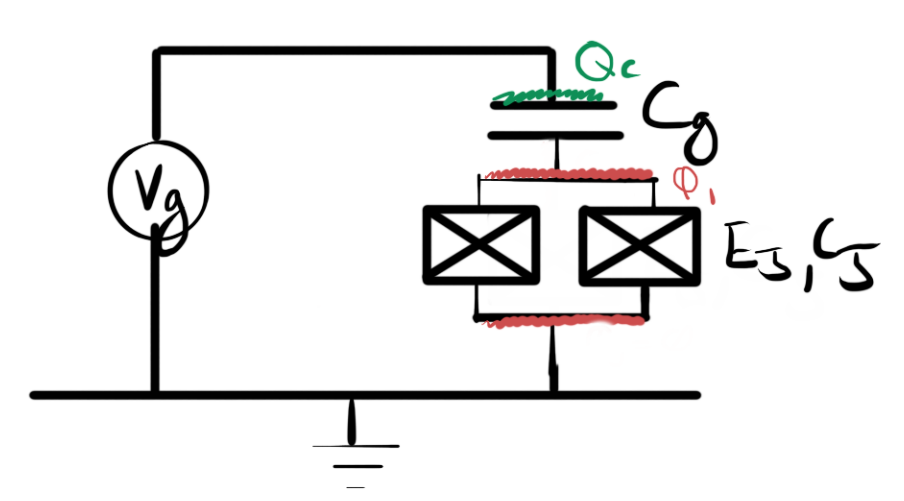
\includegraphics[height=5cm]{cooper_pair_box_4}
\end{figure}

\noindent
Adding a second JJ in parallel, will allow us to control the Josephson energy $ E_J $.
\begin{itemize}
\item    The   two    currents   throught    the   JJ    wil    give   a    total   current    \begin{equation}   I    =
    I_{c1}\sin(\phi_1)+I_{c2}\sin(\phi_2),
  \end{equation}

\item Along with the phase quantisation $ \phi_1+\phi_2+\phi_\text{ext} = 2\pi m $ and symmetric JJs $I_{c1}=I_{c2}=I_c$
  results in

  \begin{equation}
    \begin{aligned}
      I & = 2I_c\sin(\frac{\phi_1+\phi_2}{2})\cos(\frac{\phi_1-\phi_2}{2})) \\
    \end{aligned}
  \end{equation}

\begin{framed}\noindent
  Or in more general form
  \begin{equation}\label{key}
    I = I_{cs}\sin(\phi)
  \end{equation}
  \noindent where
  \begin{equation}\label{key}
    I_{cs} = 2I_c|\cos(\pi\Phi_\text{ext}/\Phi_0)|\qquad \phi = (\phi_1+\phi_2)/2
  \end{equation}

\end{framed}

\item The Josephson energy

  \begin{equation}
    \left\lbrace\begin{aligned}
        I &= I_{cs}\sin(\phi)\\
        V&=\dot{\Phi} \equiv \frac{\dot{\phi}}{2\pi}\Phi_0
      \end{aligned}\right. \Rightarrow U = \left\lbrace\begin{aligned}
        \int_{0}^{t}IV dt & = \int_{0}^{t}I_{cs}\sin(\phi)\frac{\Phi_0}{2\pi}\frac{d\phi}{dt}dt\\
        & = \int_{0}^{\phi} E_{Js}\sin(\phi)d\phi\\
        & \red{= E_{Js}(1-\cos(\phi)),\qquad E_{Js} = \frac{\Phi_0I_c}{2\pi}\times 2|\cos(\pi\Phi_\text{ext}/\Phi_0)|.}
      \end{aligned}\right.
  \end{equation}
  \begin{framed}\noindent
    \textbf{Acquires an additional factor which can now be controlled
      \begin{equation}\label{key}
        2|\cos(\pi\Phi_\text{ext}/\Phi_0)|
      \end{equation}}
  \end{framed}
\end{itemize}

\subsection{Quantising the Hamiltonian}
\subsubsection{\red{Charge energy dominates}, $ E_C/E_J >> 1$}
If charge is  the important variable, then we  chall work with the  charge basis $ \lbrace N  \rbrace $. We use the  number of phase
operators derived in App.~\ref{sec:charge_basis}

\begin{framed}\noindent

  \begin{equation}\label{key}
    \begin{aligned}
      e^{\pm i\hat{\blue{\phi}}} & = \sum_{n}\iketbra{n\pm 1}{n}\\
      \hat{\red{N}} & = \sum_{n}n\iketbra{n}{n}.
    \end{aligned}
  \end{equation}

\end{framed}

\noindent and using the exponential form of cos, we rewrite Eq.\eqref{eqn:cpbox_final}

\begin{equation}
  \begin{aligned}
    \mathcal{H} & = E_C{\left(\hat{\red{N}}-N_\text{ext}\right)^2}- E_J\cos\left(\hat{\blue{\phi}}\right)\\
    & = \sum_n\bigg[E_C{\left(n-N_\text{ext}\right)^2}\iketbra{n}{n}- \frac{E_J}{2}\bigg(\iketbra{n+1}{n}+\iketbra{n-1}{n}\bigg)\bigg]\\
    & = \begin{pmatrix}
      E_C(-2-N_\text{ext})^2 & -E_J/2 & 0 & 0 & 0\\
      -E_J/2 & \red{E_C(-1-N_\text{ext})^2} & \red{-E_J/2} & 0 & 0\\
      0 & \red{-E_J/2} & \red{E_C(N_\text{ext})^2} & -E_J/2 & 0\\
      0 & 0 & -E_J/2 & E_C(1-N_\text{ext})^2 & -E_J/2\\
      0 & 0& 0 & -E_J/2 & E_C(2-N_\text{ext})^2\\
    \end{pmatrix}
  \end{aligned}.
  \label{l2-subbed2}
\end{equation}

\begin{figure}[h]
  \centering 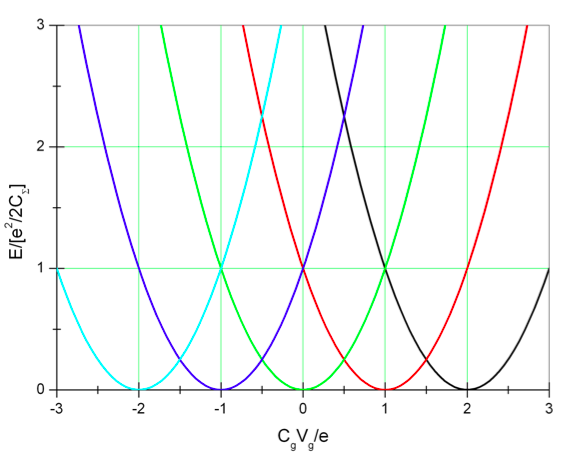
\includegraphics[height=3cm]{island}
  \caption{\small  System will  be  in the  lowest  energy  state, i.e.   have  that many  electrons  that minimize  its
    energy\label{fig:cp_box_energy_charge}}
\end{figure}

\noindent

\noindent Normally  $ N_\text{ext}  $ is  biased at a  sweet spot  \red{close to  $ - 1/2  $}. Then  the only  number of
electrons   $n$   on   out   island   that   will   give   a   low   energy   (due   to   the   energy   dispersion   in
Fig.~\ref{fig:cp_box_energy_charge}) is either  0 or -1.  The  other level will be  far separated. Then we  take out the
Hamiltonian

\red{\begin{equation}
    \begin{aligned}
      \mathcal{H}_\text{0 or -1} & = \begin{pmatrix}
        E_C(-1-N_\text{ext})^2 & -E_J/2\\
        -E_J/2 & E_C(N_\text{ext})^2\\
      \end{pmatrix}\\
    \end{aligned}
  \end{equation}}

\noindent  And  we  have  a  two  level  system  just as  in  the  previous  lecture  Eq.\eqref{l1-finalEVal}  shown  in
Fig.\ref{l2-closeup}. Redefining the zero point energy to be in the middle of the diagonal terms

\begin{equation}
  \begin{aligned}
    \mathcal{H} & = \begin{pmatrix}
      -\epsilon/2 & -E_J/2\\
      -E_J/2 & \epsilon/2\\
    \end{pmatrix}\\
    \epsilon/2    =   \frac{\text{energy    diff}}{2}    &    =   \frac{E_CN_\text{ext}^2-E_C(1+N_\text{ext})^2}{2}    =
    -\frac{E_C}{2}\big(1+2N_\text{ext}\big)
  \end{aligned}
\end{equation}

\begin{framed}\noindent
  This will have solutions

   \begin{equation}
     E = \pm \frac{\Delta E}{2}, \qquad \ket{\psi}_0 = \begin{pmatrix}
       \cos(\theta/2) \\ \sin(\theta/2)
     \end{pmatrix}, \qquad \ket{\psi}_1 = \begin{pmatrix} \sin(\theta/2) \\ \cos(\theta/2)
     \end{pmatrix}, \Delta E = \sqrt{\epsilon^2+\Delta^2}
   \end{equation}
 \end{framed}

 \begin{itemize}
 \item In  Fig.\ref{l3-energyspec} depicted  are the energy  levels for  different values of  the charging  and coupling
   energies. The stronger the coupling, $ E_J $, the bigger the splitting at the degeneracy points.

   \red{There is less charge noise in  the sweet spots of $ n_g = \mathbb{Z}\frac{1}{2} $, but  it will still be a major
     source of decoherence. \textbf{There is less dependence on charge  fluctuations as $ E_C/E_J $ gets smaller and the
       band become flatter}.}
   \begin{figure}[h]
     \centering 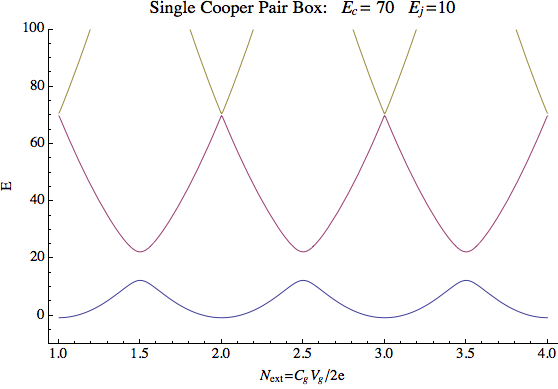
\includegraphics[height=6cm]{cpb2}
   \end{figure}

\noindent
different at the degeneracy point grows as coupling becomes stronger.\label{l3-energyspec}

\item One can also looks the ground energy state (the  one the system will most probably occupy) and find the components
  that make it up

  \[
    \Ket{\Psi}_{\text{ground}} = \sum_N\alpha_N\ket{N},
  \]

  \noindent and one sees in the  figures when there is no applied gate voltage, the island will  have $ N=0 $ charges on
  it predominantly. As one increases the gate charge, the presence of $ N=1 $ increases, until it finally dominates. The
  pattern repeats as more and more cooper pairs tunnel, to give the lowest energy configuration.

\begin{figure}[h]
  \centering 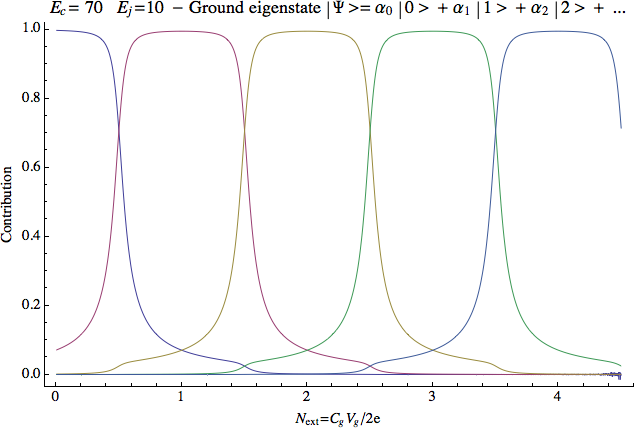
\includegraphics[height=5cm]{cpb3}
\end{figure}

\noindent
\begin{figure}[h]
  \centering 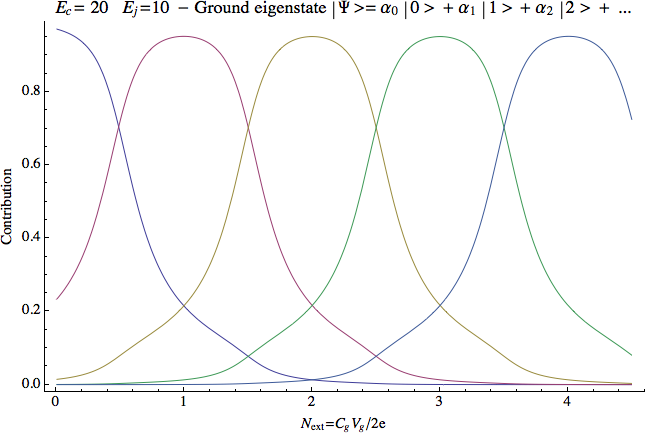
\includegraphics[height=5cm]{cpb4}
\end{figure}

\noindent

\end{itemize}

\begin{framed}\noindent
  \textbf{High $ E_C/E_J $:}
  \begin{itemize}
  \item High charge noise - gate voltage changes, affects the energy levels severely
  \item High anharmonicity - quadratic $ n $ dependance dominates, allowing individual addressing of the levels;
  \end{itemize}

\end{framed}

\newpage\subsubsection{\red{Flux energy dominates, $ E_C/E_J << 1 $}}
If flux is the important variable, then we chall work with the flux basis using the wavefunctions $ \psi(\phi) $

\begin{framed}\noindent

  \begin{equation}\label{key}
    \begin{aligned}
      &\blue{\hat{\phi}} \qquad\\
      &\red{\hat{N}} = -i\frac{d}{d\blue{\phi}}
    \end{aligned}
  \end{equation}

\end{framed}
\noindent and we rewrite

\begin{equation}\label{key}
  \begin{aligned}
    \mathcal{H} & = E_C{\left(\hat{\red{N}}-N_\text{ext}\right)^2}- E_J\cos\left(\hat{\blue{\phi}}\right)\\
    & = E_C\left(-i\frac{d}{d\phi} - n_g\right)^2 - E_J\cos(\phi).
  \end{aligned}
\end{equation}

\begin{itemize}
\item Let us compare this to Hamiltonian in a periodic potential
  \begin{equation}\label{key}
    \mathcal{H}_\text{crystal} = \frac{-\hbar^2}{2m}\frac{d^2}{dx^2}+V(x)\qquad V(x+a) = V(x),
  \end{equation}

  \noindent which, according to Bloch's theorem, states that the eigenstates will be of the form
  \begin{equation}\label{key}
    \psi_{kn}(x) = e^{ikx}u_{kn}(x),
  \end{equation}
  \noindent which, when plugged in will result in an effective Hamiltonian

  \begin{equation}\label{key}
    \mathcal{H}_{\text{eff},k} = \frac{\hbar^2}{2m}\left(-i\frac{d}{dx}+k\right)^2 + V(x)
  \end{equation}
\item We can see this mapping between
  \begin{equation}\label{key}
    \begin{aligned}
      \mathcal{H}_{\text{eff},k} & = \frac{\hbar^2}{2m}\left(-i\frac{d}{dx}+k\right)^2 + V(x)\\
      \mathcal{H} & = E_C\left(-i\frac{d}{d\phi} - n_g\right)^2 - E_J\cos(\phi),
    \end{aligned}
  \end{equation}

  \noindent so, will look for solutions of a similar form.
\item As $ E_C/E_J  $ gets smaller, the potential well  from the $ E_J\cos(\phi) $ gets  deeper \red{\textbf{and the states
      within each well localise, and  stop interacting with one another.}} Solving, as in  the Transmon Paper, will lead
  to anharmonicity relation

  \begin{framed}\noindent
    \begin{equation}\label{key} \frac{E_{12} - E_{01}}{E_{01}}\approx -(8E_J/E_C)^{-1/2},
    \end{equation}
    \noindent which decreases as we continue to increase $ E_J $.
  \end{framed}
\end{itemize}
\newpage
%
% -*- TeX-master: "../all_the_notes.tex" -*-

\
\newpage
\section{RF SQUID (Flux qubit). $ E_J/E_C\sim 50 $ \label{sec:rfSquid}}

\begin{framed}\noindent
  \noindent  The  RF SQUID  composes  of  a JJ  in  a  loop with  a  big
  inductor. \red{This inductor was neglected for the CPB in the previous
    section, since $E_C,E_J>>E_L$}.
  \begin{center}
    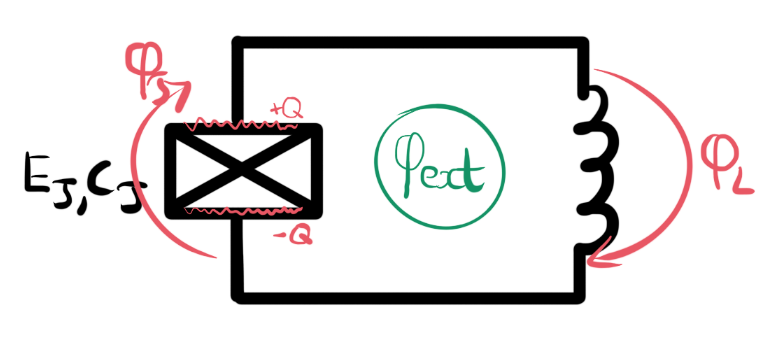
\includegraphics[height=4.5cm]{flux_1}
  \end{center}
\end{framed}



\begin{enumerate}
\item \red{\textbf{Potential  energy part}}  comes from  the JJ  and the
  inductor, where we use the phase quantisation in a loop to get

  {\begin{equation}
      \label{l3-energy1}
      \begin{aligned}
        U           =           1           -E_J\cos(\phi_J)           +
        \frac{\Phi_0^2}{(2\pi)^22L}(\phi_\text{ext}-\phi_J)^2,
      \end{aligned}
    \end{equation}}
  \begin{figure}[h]
    \centering 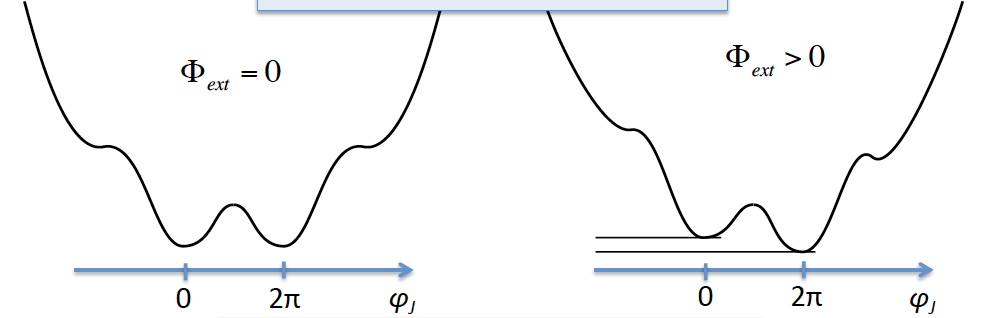
\includegraphics[height=4cm]{phij}
  \end{figure}

  \noindent
  \noindent resulting in a `wiggled' parabollic potential.

\item \red{\textbf{The charging kinetic part}} is from the voltage being
  induced by the changing flux on the JJ

  \begin{equation}\label{key}
    T = \frac{C_J}{2}\dot{\Phi}_J^2.
  \end{equation}

\item The full \red{\textbf{Lagrangian}} now reads
  \begin{equation}\label{key}
    \mathcal{L} = T - U = \frac{C_J}{2}\dot{\Phi}_J^2 + E_J\cos(\phi_J) - \frac{\Phi_0^2}{(2\pi)^22L}(\phi_\text{ext}-\phi_J)^2.
  \end{equation}

\item The \textbf{\red{conjugate momentum}}
  \begin{equation}\label{key}
    Q_J = \frac{d\mathcal{L}}{d\dot{\Phi}_J} = C_J\dot{\Phi}_J,
  \end{equation}
  \noindent is just an offset of the induced charge on the capacitor due
  to the JJ voltage.

\item So we arrive at the following set of operators

  \begin{equation}
    { \textcolor{blue}{\mathbf{x\leftrightarrow \Phi \leftrightarrow \phi} \text{ (position/flux) }}\qquad \textcolor{red}{\mathbf{p\leftrightarrow Q \leftrightarrow N \text{ (momentum/electrons) }}}}
  \end{equation}

  \noindent with the commutation relations:

  \begin{align}
    \left[\blue{x},\red{p}\right] & =i\hbar & \left[\blue{\Phi},\red{Q}\right] & = i\hbar & \left[\phi,N\right] & = \frac{2\pi}{\frac{h}{2e}}\left[\Phi,Q\right]\frac{1}{2e} = i\\
    \red{\hat{p}} & = -i\hbar\ipartial{}{\blue{x}} & \hat{\red{Q}} & =-i\hbar\ipartial{}{\blue{\Phi}} & \hat{\red{N}} & =-i\ipartial{}{\blue{\phi}}
  \end{align}

\item\

\begin{framed}\noindent
  Expressing the \red{\textbf{Hamiltonian}} in the standard fashion

  \begin{equation}
    \begin{aligned}
      \mathcal{H} & = \hat{Q}_J\dot{\hat{\Phi}}_J - \mathcal{L}\\
      & = \frac{\hat{Q}_J^2}{2C_J} - E_J\cos(\hat{\phi}_J) + \frac{\Phi_0^2}{(2\pi)^22L}(\phi_\text{ext}-\hat{\phi}_J)^2\\
      &    =   \mathbf{\red{E_C{\hat{N}^2}-    E_J\cos(\hat{\phi}_J)   +
          E_L(\phi_\text{ext}-\hat{\phi}_J)^2}}\qquad        E_c       =
      \frac{(2e)^2}{2C_J}\quad E_L = \frac{\Phi_0^2}{(2\pi)^22L}.
    \end{aligned}
  \end{equation}
\end{framed}

\item\red{\large  So now  one  has  a parabolic  potential  term in  the
    Hamiltonian, unlike in the Cooper Pair box case where there was only
    the cosine potential}
  \begin{itemize}
  \item $  \phi_{\text{ext}} $ controls  the shape of the  potential and
    hence the energies of each eigenstate
  \item $ \phi_{\text{JJ}} $ is the dynamic parameter of the qubit.
  \end{itemize}
\end{enumerate}

\newpage
\subsection{Numerical                     solution                    of
  Hamiltonian\label{subsec:flux_numerical}}
\red{Please  read  Quantum\_theory\_of\_rf\_squid,  since  this  is  all
  covered there in  great depth.}  There is a numerical  method to solve
for  the RF-SQUID,  whereby we  dice  up the  state of  the system  into
individual   values  at   discretized   positions,  with   as  step   of
$ \Delta \delta $

   \[
     \psi \rightarrow \begin{pmatrix}
       \psi(0)\\
       \psi(\Delta \delta)\\
       \psi(2\Delta \delta)\\\vdots
       \\
       \psi(n\Delta \delta)
     \end{pmatrix}
     \equiv
     \begin{pmatrix}
       w_0\\
       w_1\\
       w_2\\
       \vdots\\
       w_{n}
     \end{pmatrix}
   \]

   \noindent and solve

   % \begin{equation}\label{eqn:flux_1}
   %   \begin{aligned}
   %     \mathcal{H}\psi & = \left[\red{E_с\hat{N}^2} -
   %       \blue{E_J\cos(\hat{\phi}_J) +
   %       E_L(\phi_\text{ext}-\hat{\phi}_J)^2}\right]\psi\\
   %     & = \left[\red{-E_C\frac{\partial}{\partial\phi_J^2}} +
   %       \blue{U(\phi_J)}\right]\psi &\equiv E\psi
   %   \end{aligned}
   % \end{equation}

   \noindent  for  this   wavefunction  made  up  of  a   lot  of  small
   contributions.

\begin{figure}[h]
  \centering 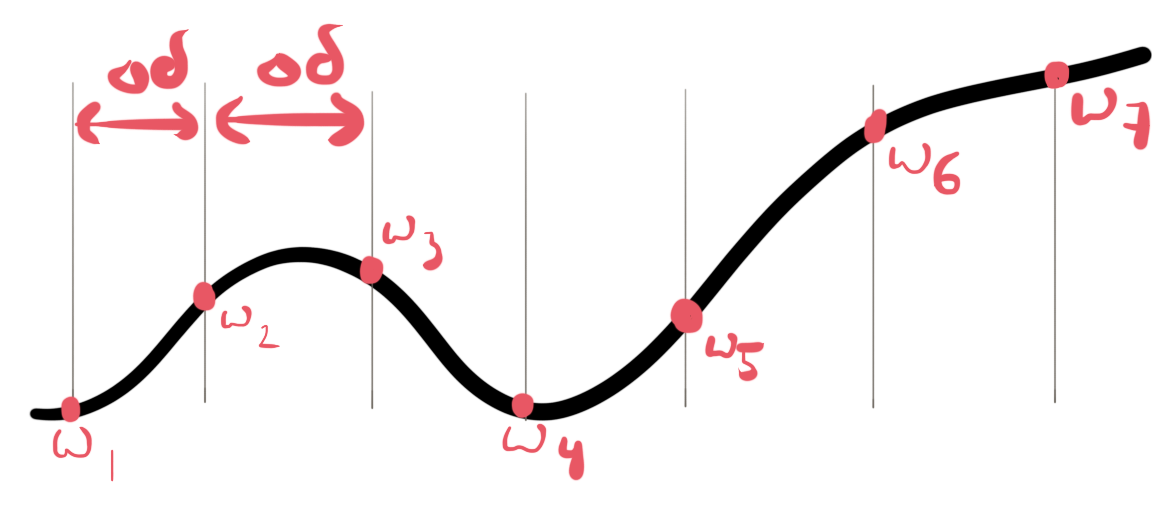
\includegraphics[height=4cm]{dicedUp}
\end{figure}

\noindent

\noindent The derivative, can be evaluated using neighbouring points:

   \begin{equation}\label{eqn:flux_2}
     \frac{d}{d\phi_J^2}\left(\omega_i\right) = \frac{\frac{\omega_{i+1} - \omega_i}{\Delta\delta} - \frac{\omega_{i} - \omega_{i-1}}{\Delta\delta}}{\Delta\delta} = \red{\frac{1}{\Delta\delta^2}\left[\omega_{i+1}+\omega_{i-1}-2\omega_{i}\right]}.
   \end{equation}

   \noindent  We  rewrite  Eq.~\eqref{eqn:flux_1}  with  the  derivative
   Eq.~\eqref{eqn:flux_2} to get
   \begin{equation}\label{key}
     \begin{aligned}
       & \left[-\frac{E_C}{\Delta\delta^2}\left[\omega_{2}+\omega_{0}-2\omega_{1}\right] + U(w_1)\right]\omega_1 = Ew_1\\
       & \left[-\frac{E_C}{\Delta\delta^2}\left[\omega_{3}+\omega_{1}-2\omega_{2}\right] + U(\omega_2)\right]\omega_2 = Ew_2\\
       & \cdots
     \end{aligned}
   \end{equation}
   \begin{framed}\noindent

     \begin{equation}\label{key}
       \begin{pmatrix}
         2\frac{E_c}{\Delta\delta^2} + U(w_1) & -\frac{E_c}{\Delta\delta^2} & 0 & 0 \\
         -\frac{E_c}{\Delta\delta^2} & 2\frac{E_c}{\Delta\delta^2} + U(w_2) &   -\frac{E_c}{\Delta\delta^2} & 0\\
         0 & -\frac{E_c}{\Delta\delta^2} & 2\frac{E_c}{\Delta\delta^2} + U(w_3) &   -\frac{E_c}{\Delta\delta^2}\\
         \vdots & \vdots & \vdots & \ddots
       \end{pmatrix}
       \begin{pmatrix}
         w_1\\w_2\\w_3\\\vdots
       \end{pmatrix}
       = E \begin{pmatrix}
         w_1\\w_2\\w_3\\\vdots
       \end{pmatrix}
     \end{equation}

     \noindent where

   \begin{equation}\label{key}
     \left[
       \begin{aligned}
         \mathbf{U(\phi_J)} & = \mathbf{E_L(\phi_\text{ext} - \phi_J)^2 - E_J\cos(\phi_J)}\\
         E_c & = \frac{(2e)^2}{2C}\\
         E_L & = \frac{\Phi_0^2}{2L(2\pi)^2}\\
         E_J         &         =        \frac{\Phi_0I_c}{2\pi}         =
         \frac{\Phi_0}{2\pi}\frac{\pi\Delta(0)}{2eR}
       \end{aligned}
     \right.
   \end{equation}
 \end{framed}

 The eigentates can be evaluated in \verb|MatLab|:
 \begin{center}
   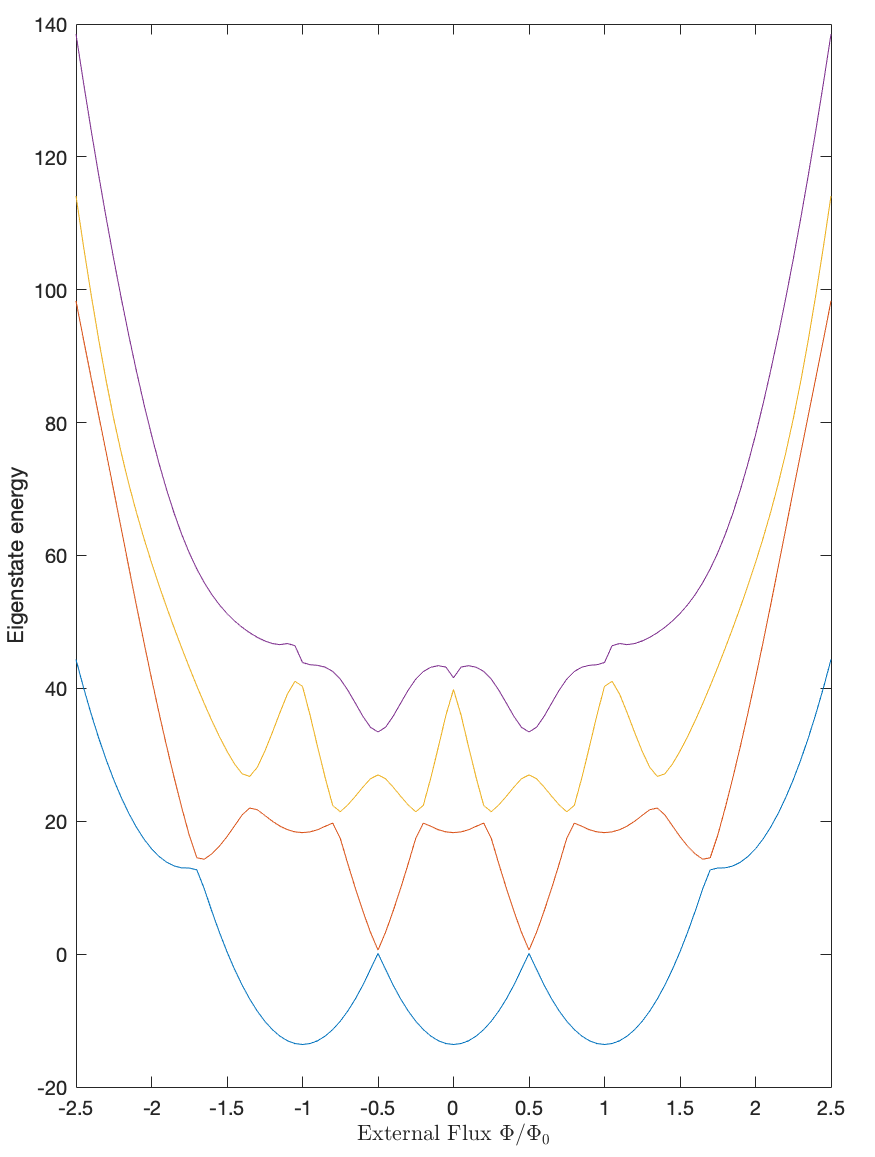
\includegraphics[height=8cm]{flux_simulation_1}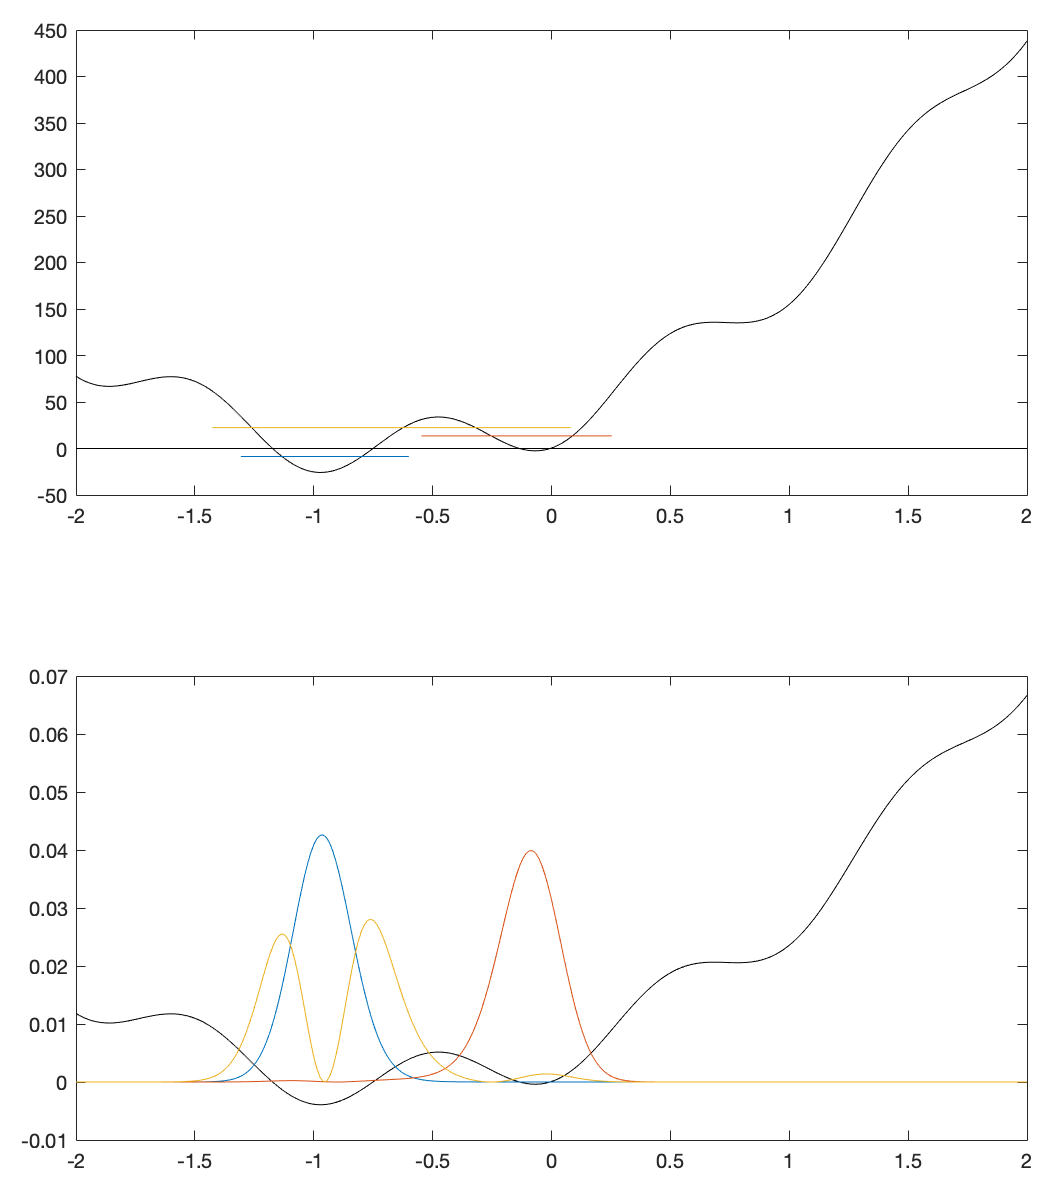
\includegraphics[height=9cm]{flux_simulation_2}
 \end{center}

 \newpage
 \subsection{Solution in the degenerate case}
 There is a  nice solution when eigenstates are  degenerate, that occurs
 with a  symmetrical double well potential.   Eigenstates \iket{\psi(0)}
 and  \iket{\psi(2\pi)}  constitute  to   the  two  circulating  current
 directions.

\begin{figure}[h]
  \centering 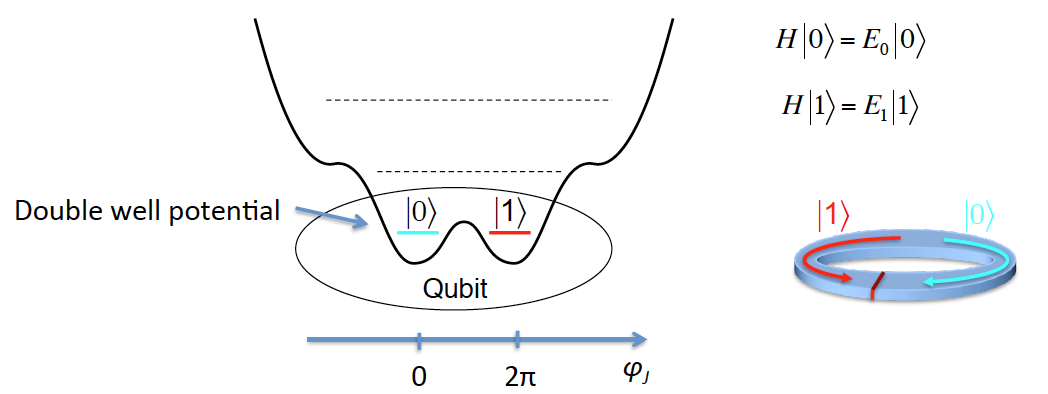
\includegraphics[height=3cm]{double}
\end{figure}

\noindent

\begin{enumerate}
\item We look for contribution to the wavefunction at $ \phi_J = 0 $ and
  $  \phi_J   =  2\pi   $,  `sampling'  much   more  strictly   than  in
  Section~\ref{subsec:flux_numerical}:
  \[
    \psi \rightarrow \begin{pmatrix}
      \psi(0)\\
      \vdots
      \\
      \psi(n\Delta \delta)
    \end{pmatrix}
    \iratext{$ \Delta = 2\pi, n = 1 $}
    \begin{pmatrix}
      \psi(0)\\
      \psi(2\pi)
    \end{pmatrix} \grey{= \psi(0)\iket{0} + \psi(2\pi)\iket{1}}
  \]

  \noindent looking for solutions to solve

  % \begin{equation}\label{}
  %   \begin{aligned}
  %     \mathcal{H}\psi & = \left[\red{E_с\hat{N}^2} -
  %       \blue{E_J\cos(\hat{\phi}_J) +
  %       E_L(\phi_\text{ext}-\hat{\phi}_J)^2}\right]\psi\\
  %     & = \left[\red{-E_C\frac{\partial}{\partial\phi_J^2}} +
  %       \blue{U(\hat{\phi}_J)}\right]\psi &&\equiv E\psi
  %   \end{aligned}
  % \end{equation}

\item The potential consists of

  \begin{equation}
    \begin{aligned}
      \blue{-E_J\cos(\phi_J)} & \rightarrow \text{ symmetric about } \phi_J = \pi(2n+1)\quad n\in\mathbb{Z}\\
      \blue{E_L(\phi_\text{ext}-\phi_J)^2} & \rightarrow \text{ symmetric about } \phi_J = \phi_\text{ext}.\\
    \end{aligned}
  \end{equation}

\item  \blue{\noindent  Thus the  potential  is  symmetrical and  states
    \iket{0} or \iket{1} are degenerate if

  \[
    \phi_\text{ext}\approx\pi+\delta\phi.
  \]}

\begin{figure}[h]
  \begin{center}
    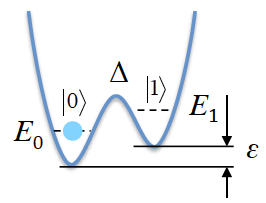
\includegraphics[height=3cm]{l3degen}
    \caption{\small  The two  lowest energies  for the  system near  the
      double potential well. The loop  is biased by a flux corresponding
      to     $\phi_\text{ext}\approx\pi$      -     half      a     flux
      quantum.\label{fig:l3degen}}
  \end{center}
\end{figure}

\item  The   energy  difference  between   the  two  wells   located  at
  $\phi_{J1}=0$ and $ \phi_{J2}=2\pi $  (or equivalently at a separation
  of 2$ \pi $).

  \begin{equation}
    \begin{aligned}
      \varepsilon &= E_0 - E_{2\pi} \\
      & = \left[-E_J\cos(0) + E_L(\phi_\text{ext}-0)^2\right] - \left[-E_J\cos(2\pi) + E_L(\phi_\text{ext}-2\pi)^2\right]\\
      & = E_L\bigg[\phi_\text{ext}^2 -\phi_\text{ext}^2 +4\pi\phi_\text{ext} -4\pi^2\bigg] =  4\pi E_L\bigg[\phi_\text{ext} -\pi\bigg]\\
      & \approx 4\pi E_L\bigg[\pi+\delta\phi -\pi\bigg] = 4\pi E_L\delta\phi = 4\pi \frac{\Phi_0^2}{(2\pi)^22L} \delta\phi = {\frac{1}{2\pi}\frac{\Phi_0^2}{2L}\delta\phi}\\
      \blue{\varepsilon} & = \blue{\frac{\Phi_0}{2L}\delta\Phi = I_p\delta\Phi}\\
      & \red{\text{Recalling that } E_J = \frac{\Phi_0 I_c}{2\pi}, \text{ where $ I_c $ is the maximal persistent current (critical current)}}\\
    \end{aligned}
  \end{equation}

  \begin{framed}\noindent
  \item   So  for   the  potential   part  accounts   for  two   states,
    \iket{\psi(0)}  and  \iket{\psi(2\pi)}  at two  different  energies,
    which we can write as a diagonal matrix

  \begin{equation}\label{key}
    \blue{U =
      \kbordermatrix{
        & \iket{\psi(0)} & \iket{\psi(2\pi)}\\
        \bra{\psi(0)} & \frac{\varepsilon}{2} & 0\\
        \bra{\psi(2\pi)} & 0& -\frac{\varepsilon}{2}\\
      } \qquad \qquad \varepsilon = \frac{\Phi_0}{2L}\delta\Phi = I_p\delta\Phi}.
  \end{equation}

\end{framed}

\item                The                \red{kinetic                term
    $ \red{-E_C\frac{\partial}{\partial\phi_J^2}}  $} is evaluted  as in
  Chapter~\ref{subsec:flux_numerical}

  \begin{equation}\label{}
    \begin{aligned}
      \frac{d}{d\phi_J^2}\omega_i & = \frac{\frac{\omega_{i+1} - \omega_i}{\Delta\delta} - \frac{\omega_{i} - \omega_{i-1}}{\Delta\delta}}{\Delta\delta} = \red{\frac{1}{\Delta\delta^2}\left[\omega_{i+1}+\omega_{i-1}-2\omega_{i}\right]}\\
      \bullet \frac{d}{d\phi_J^2}\psi(0) & = \frac{1}{(2\pi)^2}\left[\psi(2\pi) + \grey{\psi(-2\pi)} - 2\psi(0)\right] \grey{\approx} \frac{1}{4\pi^2}\left[\psi(2\pi) - 2\psi(0)\right]\\
      \bullet\frac{d}{d\phi_J^2}\psi(2\pi)              &              =
      \frac{1}{(2\pi)^2}\left[\grey{\psi(4\pi)}     +    {\psi(0)}     -
        2\psi(2\pi)\right]  \grey{\approx} \frac{1}{4\pi^2}\left[\psi(0)
        - 2\psi(2\pi)\right],
    \end{aligned}
  \end{equation}

  \noindent  where we  assume  that  for the  lowest  energy states  the
  wavefucntion      is      negligible       outside      the      well:
  $ \psi(4\pi) = \psi(-2\pi) = 0 $.

\item In matrix form this looks like

  \begin{equation}\label{key}
    \red{-E_C\frac{d}{d\phi_J^2} = \kbordermatrix{
        & \iket{\psi(0)} & \iket{\psi(2\pi)}\\
        \bra{\psi(0)} & \frac{1}{4\pi^2}2E_C & -\frac{1}{4\pi^2}E_C\\
        \bra{\psi(2\pi)} & -\frac{1}{4\pi^2}E_C& \frac{1}{4\pi^2}2E\\
      } \equiv \kbordermatrix{
        & \iket{\psi(0)} & \iket{\psi(2\pi)}\\
        \bra{\psi(0)} & 0 & -\frac{\Delta}{2} \\
        \bra{\psi(2\pi)} & -\frac{\Delta}{2}& 0\\
      }\qquad\Delta = \frac{2E_C}{4\pi^2}	}
  \end{equation}

\item\

\begin{framed}\noindent
  The Hamiltonian can be written as that for a two level system

  \begin{equation}
    \begin{aligned}
      \mathcal{H} &\approx -\frac{\varepsilon}{2}\sigma_z - \frac{\Delta}{2}\sigma_x = \kbordermatrix{ &  \iket{\psi(0)} & \iket{\psi(2\pi)}\\
        \bra{\psi(0)} & -\varepsilon/2  & -\Delta/2\\ \bra{\psi(2\pi)} &
        -\Delta/2& \varepsilon/2 }
      \qquad \red{\text{when } \phi_\text{ext} \approx\pi} \\
      \varepsilon & = \frac{\Phi_0}{2L}\delta\Phi  \qquad\qquad \text{controlled by bias flux}\\
      \Delta  &   =  \frac{2E_C}{4\pi^2}  \qquad\qquad\text{anticrossing
        energy between states \iket{0} and \iket{1}}
    \end{aligned}
  \end{equation}
\end{framed}

\item  Solving  as  in Chapter~\ref{sec:firstLecture}  using  a  unitary
  rotation
  \begin{equation}
    \label{l1-newH}
    \begin{aligned}
      \mathcal{H} & = {-\frac{\epsilon}{2}\sigma_z-\frac{\Delta}{2}\sigma_x}\\
      & = -\frac{\sqrt{\epsilon^2+\Delta^2}}{2}\left(\frac{\epsilon}{\sqrt{\epsilon^2+\Delta^2}}\sigma_z+\frac{\Delta}{\sqrt{\epsilon^2+\Delta^2}}\sigma_x\right)\\
      & = -\frac{\Delta E}{2}\left(\cos\left(\theta\right)\sigma_z+\sin\left(\theta\right)\sigma_x\right)\\
      \Delta E & = \sqrt{\epsilon^2+\Delta^2}\\
      \tan(\theta) & = \frac{\Delta}{\epsilon}\\
    \end{aligned},
  \end{equation}
  \noindent  with  eigenvectors  and  eigenvalues  being  a  mixture  of
  persistence       current        states       \iket{\circlearrowleft},
  \iket{\circlearrowright}.

 \begin{equation}\label{key}
   E = \pm \frac{\Delta E}{2}, \qquad \ket{0} = \begin{pmatrix}
     \cos(\theta/2) \\ \sin(\theta/2)
   \end{pmatrix},  \qquad \ket{1}  =  \begin{pmatrix} \sin(\theta/2)  \\
     -\cos(\theta/2).
   \end{pmatrix}
 \end{equation}
\item  With   states  \iket{\circlearrowleft}   $  \equiv  +I_p   $  and
  $ \iket{\circlearrowright} \equiv -I_p $ the expectation values of the current:
  \begin{equation}\label{key}
    \begin{aligned}
      \iaverage{I}_{\iket{0}} & = I_p\cos(\theta/2)^2 - I_p \sin(\theta/2)^2 = I_p\cos(\theta)\\
      \iaverage{I}_{\iket{1}} & = I_p\sin(\theta/2)^2 - I_p \cos(\theta/2)^2 = - I_p\cos(\theta)\\
    \end{aligned}
  \end{equation}
\item  Now  we   perform  a  transformation  to  rotate   the  state  by
  $ 2\alpha = \theta $

 \begin{equation}
   \mathbf{U=e^{i\frac{\theta}{2}\sigma_y}} =  \cos(\alpha)\mathbb{I}+i\sin(\alpha)\sigma_y
 \end{equation}

 \noindent to rotate the basis in this plane. \red{\textbf{Note that the
     transformation uses an angle HALF of the required turn}}. The {time
   independent   Hamiltonian}   will   be   transformed   according   to
 Eq.\eqref{uninewschrodinger},  and  evaluating  using  the  commutation
 relations Eq.\eqref{uniComm1}

 \begin{equation}
   \begin{aligned}
     \mathcal{H}' & = U\mathcal{H}U^{\dagger} = U \bigg[-\frac{\Delta E}{2}\big(\sigma_z\cos(\theta)+\sigma_x\sin(\theta)\big)\bigg]\bigg[\cos(\theta/2)\mathbb{I}\red{-}i\sin(\theta/2)\sigma_y\bigg]\\
     & = U \bigg[\cos(\theta/2)\mathbb{I}+i\sin(\theta/2)\sigma_y\bigg]\bigg[-\frac{\Delta E}{2}\big(\sigma_z\cos(\theta)+\sigma_x\sin(\theta)\big)\bigg]\\
     & = UU\mathcal{H} =-\frac{\Delta E}{2} \bigg[\cos(\theta)\mathbb{I}+i\sin(\theta)\sigma_y\bigg]\bigg[\big(\sigma_z\cos(\theta)+\sigma_x\sin(\theta)\big)\bigg]\\
     & = -\frac{\Delta E}{2}\bigg[\cos^2(\theta)\sigma_z+\sin(\theta)\cos(\theta)\sigma_x+i\sin(\theta)\cos(\theta)\red{\sigma_y\sigma_z}+i\sin^2(\theta)\red{\sigma_y\sigma_x}\bigg]\\
     & = -\frac{\Delta E}{2}\bigg[\cos^2(\theta)\sigma_z+\sin(\theta)\cos(\theta)\sigma_x+i\sin(\theta)\cos(\theta)\red{i\sigma_x}+i\sin^2(\theta)\red{-i\sigma_z}\bigg]\\
     & = -\frac{\Delta E}{2}\sigma_z,
   \end{aligned}
 \end{equation}

\item\

  \begin{framed}\noindent
    \noindent In the rotated frame we have a two level system, where the
    biasing flux, and the anticrossing  energies come together to create
    new system eigenstates:

    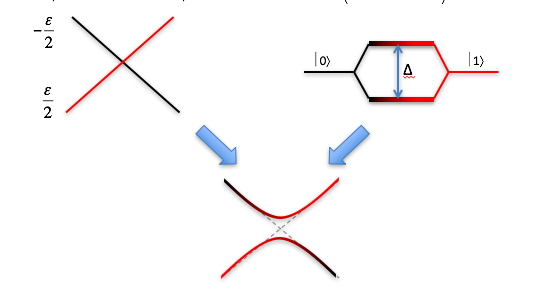
\includegraphics[height=5cm]{together}

    \noindent

  \begin{equation}\label{key}
    \mathcal{H'} = -\frac{\Delta E}{2}\sigma_z
  \end{equation}

  \red{With eigenstates  $ \iket{\psi(0)},  \iket{\psi(2\pi)} $  (mix of
    persistent current states) at energies
    \begin{equation}\label{key}
      \pm\frac{\Delta E}{2} \qquad \Delta E = \sqrt{\varepsilon^2 + \Delta^2}\qquad\varepsilon = \frac{\Phi_0}{2L}\delta\Phi  \qquad	\Delta = \frac{2E_C}{4\pi^2}.
    \end{equation}
  }
\end{framed}
\end{enumerate}

\noindent Fig.\ref{fig:l3wavefun} depicts the approximated wavefunctions
and Fig.\ref{fig:l3energy} the energies for different external fields.

\begin{figure}[h]
  \centering 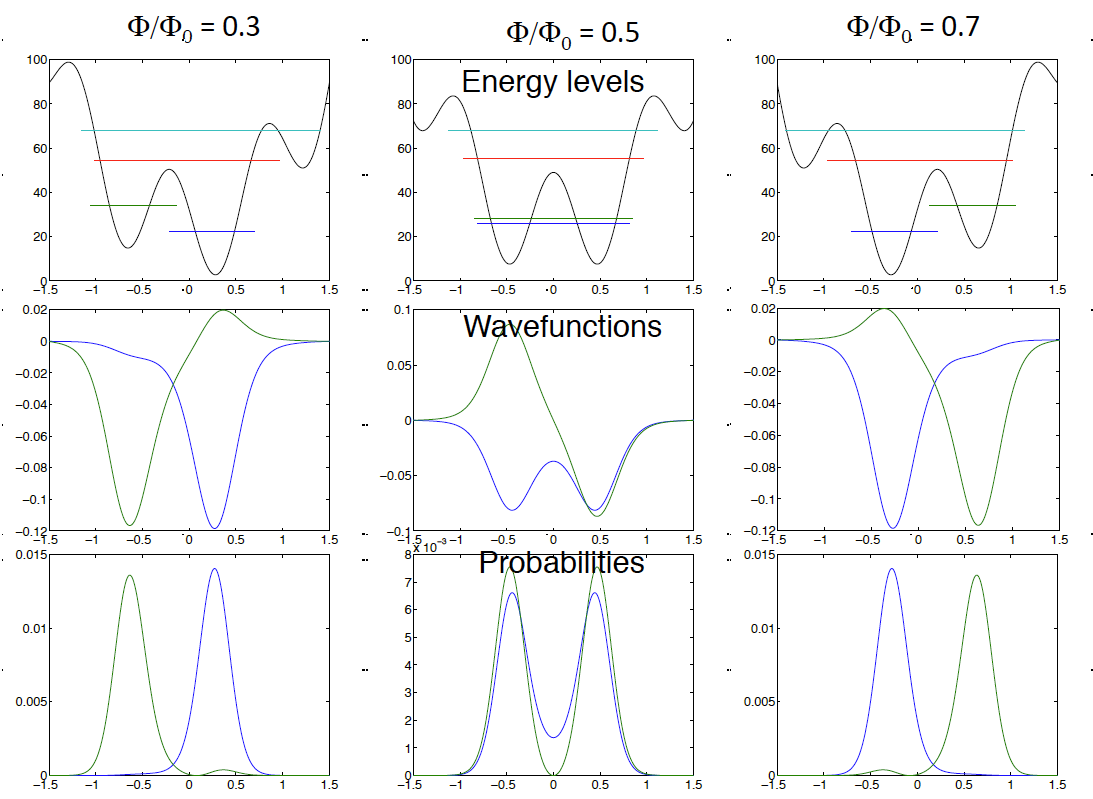
\includegraphics[height=10cm]{l3wavefun}
  \caption{The wavefunctions of  the RF SQUID as a  function of $\phi_J$
    for different  external flux  $\phi_\text{ext}$ biases.   Notice how
    the different flux  biases change the symmetry of  the potential and
    the shape of the wavefunctions}
  \label{fig:l3wavefun}
\end{figure}

\begin{figure}[h]
  \begin{center}
    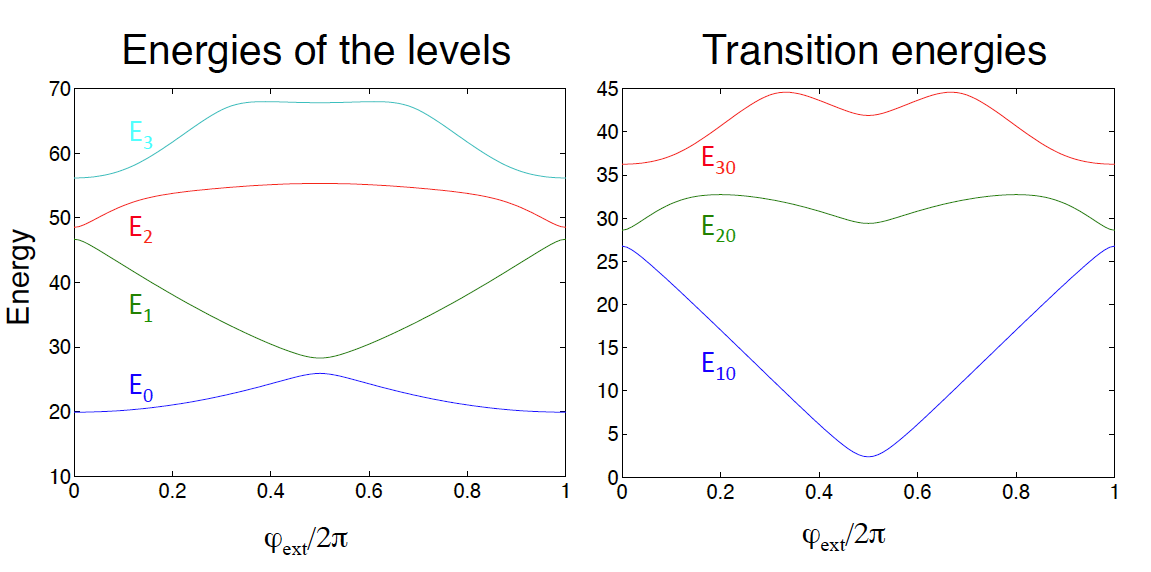
\includegraphics[height=7cm]{l3energy}
    \caption{\small  The  energy  levels  and  their  differences  as  a
      function of  the \textbf{applied flux} $\phi_\text{ext}$.   At the
      degeneracy      point,       the      levels       come      close
      together.\label{fig:l3energy}}
  \end{center}
\end{figure}

\newpage

 \subsection{Question about fabrication}
 There is a technological limitation to  this kind of device. Once needs
 a  large  inductance $L$,  but  be  able  to  keep a  relatively  small
 size. Otherwise  the capacitance $ C  $ of the system  grows too large,
 which prevents the tunnelling of the localised states.

 A  proposal is  to  replace the  classical inductor  with  a JJ,  which
 provides plenty of inductance, while keeping a considerable size.  Will
 it work?  Lets evaluate the potential energy

 \begin{equation}
   \left\lbrace\begin{aligned}
       U^{\text{potential}} & = -E_J\cos(\phi_{J1}) - \alpha E_J\cos(\phi_{J2})\\
       \phi_{J1} - \phi_{J2} & = \phi_\text{ext}
     \end{aligned}\right. \Rightarrow
   \begin{aligned}
     &-E_J\cos(\phi_{J1}) - \alpha E_J\cos(\phi_{J1}-\phi_\text{ext})\\
     & = -E_J\bigg[\cos(\phi_{J1}-\frac{\phi_\text{ext}}{2}+\frac{\phi_\text{ext}}{2}) + \alpha\cos(\phi_{J1}-\frac{\phi_\text{ext}}{2}-\frac{\phi_\text{ext}}{2})\bigg]\\
     & = -E_J\bigg[\cos(\phi'+\frac{\phi_\text{ext}}{2}) + \alpha\cos(\phi'-\frac{\phi_\text{ext}}{2})\bigg]\\
     & = -E_J\bigg[\cos(\phi')\cos(\frac{\phi_\text{ext}}{2}) + \alpha\cos(\phi')\cos(\frac{\phi_\text{ext}}{2})\\
     & - \sin(\phi')\sin(\frac{\phi_\text{ext}}{2}) + \alpha\sin(\phi')\sin(\frac{\phi_\text{ext}}{2}) \bigg]\\
     &                                                           \approx
     -E_J(1+\alpha)\bigg[\cos(\phi')\cos(\frac{\phi_\text{ext}}{2})\bigg]
   \end{aligned}
 \end{equation}

 \noindent There is no parabolic dependence, making the localised states
 unsuitable -  the eigenstates  will tunnel across  all of  the possible
 wells formed by  the cosine potential. \textbf{So this  is not possible
   with just replacing an inductor with a JJ.}

 \newpage
%
\section{3 JJ qubit \label{subsec:l33jj}}
 \iframe{
 	From \cite{gu2017}:
 	\begin{itemize}
 		\item To create a double potential well we need $ \alpha > 0.5 $ and to reduce flux noise we need $ \alpha < 0.7 $;
 	\end{itemize}
 }
  For this model we put 3 JJ in a loop, all with a parallel capacitor as shown in Fig.\ref{fig:l33jja}.
  
  \begin{figure}[h]
  	\ipic{4cm}{3jj}
  	\label{fig:l33jj}
  \end{figure}
  
  \begin{enumerate}
  	\item \textbf{\red{Potential energy}} comes from all three JJs, where we denote the phases
  
  \begin{equation}
	  e^{i\phi_{01}} = e^{i(\phi_0-\phi_1)}
  \end{equation}
  
  \blue{\begin{equation}
  	\begin{aligned}
	  	U_{\text{potential}} & = E_J(1-\cos(\phi_{01})) + \alpha E_J(1-\cos(\phi_{12})) + E_J(1-\cos(\phi_{20}))\\
	  	& = E_J\bigg[2+\alpha - \cos(\phi_{01}) - \cos(\phi_{20}) - \alpha\cos(\phi_\text{ext}-\phi_{01} - \phi_{20})\bigg].
  	\end{aligned}
  \end{equation}}
    
  \begin{center}
  	\ipic{4cm}{3jjc}
  	\ipic{5cm}{3jj1}
  	\ipic{5cm}{3jj2}
  	\captionof{figure}{$\alpha$ determines the height of the barrier in the middle of the two wells. Larger alpha raises the barrier up. $ \phi_\text{ext} $ determines the symmetry of the wells (as in the previous section).}
  	\label{fig:l33jjc}
  \end{center}
  
   \item \red{\textbf{The kinetic energy}} comes from the charging energy. Its better to work with the capacitance matrix for the system which links a given charge vector $ \vec{n} $ with a potential vector $ \vec{V} $, the circuit is summarised in Fig.\ref{fig:l33jja}
  
  \begin{equation}
	  \left\lbrace \begin{aligned}
		  \vec{n} & = \left(\begin{smallmatrix}
		  n_1\\n_2
		  \end{smallmatrix}\right)\\
		  \vec{V} & =\left(\begin{smallmatrix}
		  V_1\\V_2
		  \end{smallmatrix}\right)\\
		  C & = \left(\begin{smallmatrix}
		  C_{01}+C_{12} & -C_{12}\\-C_{12} &C_{02}+C_{12}
		  \end{smallmatrix}\right)\\
	  \end{aligned}\right. \Rightarrow \vec{n} = \frac{C\vec{V}}{2e} \equiv \begin{bmatrix}
	  	C_{01}\left(V_1-0\right) + C_{12}\left(V_1-V_2\right)\\ 	C_{01}\left(V_2-0\right) + C_{12}\left(V_2-V_1\right)
	  \end{bmatrix},
  \end{equation}
  
  \noindent which is just the typical evaluating of charge on a capacitor from $ Q = CV $. For evaluating the kinetic energy from the charges
  
  \begin{equation}
	  \left\lbrace \begin{aligned}
		  \vec{V} & = 2eC^{-1}\vec{n}\\
		  \vec{Q} & = 2e\vec{n}\\
		  \red{U_{\text{kinetic}}} & \red{= \frac{1}{2}Q.V}\\
	  \end{aligned}\right. \Rightarrow \red{U_{\text{kinetic}} = \frac{1}{2}\left(2e\vec{n}^{\text{T}}\right)\left(2eC^{-1}\vec{n}\right) = \frac{(2e)^2}{2}\vec{n}^{\text{T}}C^{-1}\vec{n}},
  \end{equation}
  
  
   \item The total Hamiltonian for the 3JJ/3 capacitor system being
  
  \begin{equation}
  	\label{eqn:l23JJ}
  	\mathcal{H} = \red{U_{\text{kinetic}}} + \blue{U_{\text{potential}}} = \red{\frac{(2e)^2}{2}\vec{n}^{\text{T}}C^{-1}\vec{n}} + \blue{E_J\bigg[2+\alpha - \cos(\phi_{01}) - \cos(\phi_{20}) - \alpha\cos(\phi_\text{ext}-\phi_{01} - \phi_{20})\bigg]}.
  \end{equation}
  
  For simple representation in matrix form, we write it out in the \textbf{charge basis}. In such a basis (recall from Eq.\eqref{l2-phase} for the one island case) we have the results summarised in Table \ref{tab:phaseChange}.
  
  {\begin{table}[h]
  	\label{tab:phaseChange}
  	\caption{Note how the phase operators increase and decrease the islands associated to a given phase.}
  	\begin{center}
	  {\footnotesize \begin{tabular}{|c|c|}
	  	\hline
	  	\textbf{One island} (Sec.\ref{subsec:l2-CPB}) & Two islands\\\hline
	  	 $ \hat{N} = \sum_N\ketbra{N}{N} $ & $ \frac{(2e)^2}{2}\begin{pmatrix}
	  	n_1 & n_2
	  	\end{pmatrix}C^{-1}\begin{pmatrix}n_1 \\ n_2\end{pmatrix} =  \displaystyle\sum_{N_1,N_2}\mathbf{U}(n_1,n_2)\ketbra{n_1,n_2}{n_1,n_2} $\\\hline
	  	\multirow{3}{*}{$ e^{i\phi}  = \sum_N\ketbra{N+1}{N}$} & $ e^{i\phi_{01}} = e^{i(\phi_{0}-\phi_1)} =  \displaystyle\bigg[\sum_{n_1}\ketbra{n_1-1}{n_1}\bigg]\otimes \red{\bigg[\sum_{n_\text{ground}}\ketbra{n_\text{ground}+1}{n_\text{ground}}\bigg] - \text{ ignore}}$\\
	  	& $ e^{-i\phi_{01}} = e^{i(\phi_{1}-\phi_0)} =  \displaystyle\sum_{n_1}\ketbra{n_1+1}{n_1}$\\
	  	& $ e^{i\phi_{20}} = e^{i(\phi_{2}-\phi_0)} =  \displaystyle\sum_{n_2}\ketbra{n_2+1}{n_2}$\\
	  	\multirow{3}{*}{$ e^{-i\phi}  = \sum_N\ketbra{N-1}{N}$} & $ e^{-i\phi_{20}} = e^{i(\phi_{0}-\phi_2)} =  \displaystyle\sum_{n_2}\ketbra{n_2-1}{n_2}$\\
	  	 & $ e^{i\phi_{12}} (\equiv e^{\phi_\text{ext}-\phi_{01}-\phi_{20}}) = e^{i(\phi_1-\phi_2)} =  \displaystyle\bigg[\sum_{n_1}\ketbra{n_1+1}{n_1}\bigg]\otimes {\bigg[\sum_{n_2}\ketbra{n_2-1}{n_2}\bigg]} $\\
	  	 & $ e^{-i\phi_{12}} = e^{i(\phi_2-\phi_1)} =  \displaystyle\bigg[\sum_{n_1}\ketbra{n_1-1}{n_1}\bigg]\otimes {\bigg[\sum_{n_2}\ketbra{n_2+1}{n_2}\bigg]} $\\\hline
	  \end{tabular}}
  	\end{center}
  \end{table}}

   \item  We draw parallels to rewrite our new Hamiltonian in matrix form (using exponential form of trigonometric functions and zeroing constant offsets and replacing the last exponential with explicit dependence on the phase across the junction)
  
  \begin{equation}
   \label{eqn:l3ToMatrixForm}
   \begin{aligned}
 	 \mathcal{H}  = \red{\frac{(2e)^2}{2}\vec{n}^{\text{T}}C^{-1}\vec{n}} & - \blue{\frac{E_J}{2}\big(e^{i\phi_{01}}+e^{-i\phi_{01}}\big) - \frac{E_J}{2}\big(e^{i\phi_{20}}+e^{-i\phi_{20}}\big) - \frac{\alpha E_J}{2}\big(e^{i\phi_{12}}+e^{-i\phi_{12}}\big)}\\\\
    \Rightarrow \sum_{n_1,n_2} \red{U(n_1,n_2)\ketbra{n_1,n_2}{n_1,n_2}} & \\
    & \blue{ - \frac{E_J}{2}\bigg[\ketbra{n_1-1}{n_1}+\ketbra{n_1+1}{n_1}\bigg]\otimes \mathbb{I}_2}\\
    & \green{- \frac{E_J}{2} \mathbb{I}_1\otimes\bigg[\ketbra{n_2+1}{n_2}+\ketbra{n_2-1}{n_2}\bigg]}\\
    & \purple{- \frac{\alpha E_J}{2}\bigg[\ketbra{n_1+1}{n_1}\ketbra{n_2-1}{n_2}+\ketbra{n_1-1}{n_1}\ketbra{n_2+1}{n_2}\bigg]}\\
    \Rightarrow \sum_{n_1,n_2} \red{U(n_1,n_2)\ketbra{n_1,n_2}{n_1,n_2}} & \\
    & \blue{ - \frac{E_J}{2}\bigg[\ketbra{n_1-1,\mathbf{n_2}}{n_1,\mathbf{n_2}}+\ketbra{n_1+1,\mathbf{n_2}}{n_1,\mathbf{n_2}}\bigg]\ra \text{ $n_2$ constant}}\\
    & \green{- \frac{E_J}{2} \bigg[\ketbra{\mathbf{n_1},n_2+1}{\mathbf{n_1},n_2}+\ketbra{\mathbf{n_1},n_2-1}{\mathbf{n_1},n_2}\bigg]\ra \text{ $n_1$ constant}}\\
    & \purple{- \frac{\alpha E_J}{2}\bigg[\ketbra{n_1+1,n_2-1}{n_1,n_2}+\ketbra{n_1-1,n_2+1}{n_1,n_2}\bigg]}
   \end{aligned}
  \end{equation}
 
  \noindent and writing out in matrix form
  
  \begin{equation}
  	\mathcal{H} = \kbordermatrix{
  	 & \ket{-1,0} & \ket{0,-1} & \ket{0,0} & \ket{0,1} & \ket{1,0}\\
  	 \bra{-1,0} &\red{ U(-1,0)} & \purple{-\frac{E_J}{2}} & \blue{-\frac{E_J}{2}} & 0 & 0\\
  	\bra{0,-1} & \purple{-\frac{E_J}{2}} & \red{U(0,-1) } & \green{-\frac{E_J}{2}} & 0 & 0\\
  	\bra{0,0} & \blue{-\frac{E_J}{2}} & \green{-\frac{E_J}{2}} & \red{U(0,0)} & \green{-\frac{E_J}{2}} & \blue{-\frac{E_J}{2}}\\
  	\bra{0,1} & 0 & 0 & \green{-\frac{E_J}{2}} & \red{U(0,1) }& \purple{-\frac{E_J}{2}}\\
  	\bra{1,0} & 0 & 0 & \blue{-\frac{E_J}{2}} & \purple{-\frac{E_J}{2}} & \red{U(1,0)}\\
  	}
  \end{equation}
    \end{enumerate}

  \begin{center}
  	\ipic{6cm}{3jja}
  	\label{fig:l33jja}
  	\captionof{figure}{System of tunnelling electrons between the three junctions}
  \end{center}



\newpage

%
% -*- TeX-master: "../all_the_notes.tex" -*-
\newpage
\section{4JJ-series Flux Qubit \cite{qui2016}}
\iframe{This qubit behaves like a 3JJ qubit, albeit with some \red{differences}:
  \begin{itemize}
  \item Can be operated in the single or double potential well regime;
  \item \red{Has a lower flux sensitivity and thus better to tune};
  \item \red{Under  certain conditions  \textbf{only \iket{1}\lra\iket{2}} allowed.   In other
      systems other transitions are also possible} - no state leakage to \iket{3}.
  \end{itemize}}

\noindent
\subsection{Derivation of the Hamiltonian}
It's a load of bloat including:
\begin{enumerate}
\item Using phase loop quantisation
  \begin{equation}\label{key}
    \varphi_1 + \varphi_2 + \varphi_\alpha + \varphi_\beta + 2\pi f_\text{tot} = 0;
  \end{equation}
\item Kinetic energy evaluation, using emf induction $ V = \dot{\Phi} $:
  \begin{equation}\label{key}
    \begin{aligned}
      \mathcal{T} = & \frac{1}{2}\sum C_iV_i^2\\
      &   =   \frac{C}{2}\left(\frac{\Phi_0}{2\pi}\right)^2\left\lbrace\dot{\varphi}^2_1    +   \dot{\varphi}^2_2   +
        \alpha\dot{\varphi}^2_\alpha    +     \beta\left[\dot{\varphi}_1    +    \dot{\varphi}_2    +     \dot{\varphi}_\alpha    +    2\pi
          \dot{f}_\text{tot}\right]^2\right\rbrace;
    \end{aligned}
  \end{equation}
\item Potential energy
  \begin{equation}\label{key}
    U = \sum E_{Ji}\left[1 - \cos(\varphi_i)\right].
  \end{equation}
\item Inductive energy
  \begin{equation}\label{key}
    U_L = \frac{\Phi_0^2}{2L}\left(f_\text{tot} - f_\text{ext}\right)^2.
  \end{equation}
\item Some complicated transformation that maps $ \varphi_1, \varphi_2, \varphi_\alpha \ra \varphi_+, \varphi_-, \varphi, \xi $, where
  \begin{equation}\label{key}
    \xi = f_\text{tot} - f_e \approx f_a(t)\ (\text{negligible flux linxed by current}),
  \end{equation}
  \ipic{5cm}{flux4jj_1}
  \noindent is the time dependent component of the magnetic field to arrive at the largrangian
  \begin{equation}\label{key}
    \begin{aligned}
      \mathcal{L} & = \mathcal{T} - U\\
      & =  \frac{C}{2}\left(\frac{\Phi_0}{2\pi}\right)^2\left(\dot{\varphi}^2 + \Gamma_+\dot{\varphi}_+^2 + \Gamma_-\dot{\varphi}_-^2 + \Gamma_\xi\xi^2\right)\\
      & - U(\varphi, \varphi_+, \varphi_-, \xi) - \frac{\Phi_0^2}{2L}\left(\xi - f_\text{a}\right)^2
    \end{aligned}
  \end{equation}
\item Finding the canonical momenta
  \begin{equation}\label{key}
    P_i = \difffrac{\mathcal{L}}{\varphi_i}
  \end{equation}
  	
  \noindent and evaluating the Hamiltonian, $ \mathcal{H} = \sum P_i\varphi_i - \mathcal{L} $.
\item Splitting the Hamiltonian up into a Harmonic oscillator part
  \begin{equation}\label{key}
    \mathcal{H} = 4E_C\left(P^2 + \frac{P_+^2}{\Gamma_+} + \frac{P_-^2}{\Gamma_-}\right) + U(\varphi, \varphi_+, \varphi_-, \xi) + \red{\mathcal{H}_\text{osc}},
  \end{equation}
  	
  \noindent \red{which is always in the ground state, due to its energy being much higher than
    the qubit levels. Thus it can be dropped from consideration.}
\end{enumerate}

\subsection{Bloat over}
So now lets have a look at some implications of this Hamiltonian.
 
\begin{enumerate}
\item  \textbf{The potential  landscape that  forms} has  adjustable single  and double  wells
  through $ \beta $.  \iframe{\red{Double well for $ \beta > 0.3 $, which is much broader than the 0.5
      threshold in 3 JJ qubit.}}  \ipic{6cm}{flux4jj_2}
\item The solution of $ \mathcal{H}_0\psi(\mathbf{\varphi}) = E\psi(\mathbf{\varphi}) $ is looked for in a block
  wave form
  \begin{equation}\label{key}
    \Psi(\mathbf{\varphi}) = u(\mathbf{\varphi}) = \sum_{\mathbf{K}}a_\mathbf{K}e^{i\mathbf{K}.\mathbf{\varphi}}.
  \end{equation}
 	
\item In the single well configuratio (\textbf{bottom}, $ \beta < 0.3 $) the bands are flatter and
  less susceptible to flux noise than in the double well (\textbf{top}, $ \beta > 0.3 $) case.
 	
  \ipic{7cm}{flux4jj_3} \iframe{Note  the superior separation  of the  levels in both  the 3JJ
    (left) and 4JJ (right) qubits. So energy structure is preserved, and that is good.}
 	
\item \iframe{\red{\textbf{The addition  of a time dependent field changes  the hamitlonian to
        give a perturbation}}:
    \begin{equation}\label{key}
      \begin{aligned}
        \mathcal{H} & = \mathcal{H}_0 - I\Phi_a(t)\\
        & I = \text{ effective current, which is a monster of an equation}\\
        & \Phi_a(t) = \iabs{\Phi_a}\cos(\omega_at).
      \end{aligned}
    \end{equation}
 	
    \noindent  and we  have a  transition  that is  calculated  using the  eigenstates of  the
    original Hamiltonian
 	
 	\begin{equation}\label{key}
          t_{ij} = \bra{i}I\Phi_a\ket{j}.
 	\end{equation}}
    \item The results are:
      \begin{itemize}
      \item At the  degeneracy point, \iket{1}\lra\iket{3} is  forbidden, and we have a  $ \Xi $
        energy  ladder.  Everywhere  else it's  a  $ \Delta  $ configuration  with all  transitions
        allowed.  \ipic{6cm}{flux4jj_4}
      \item  For  low  $  \beta  $ all  transitions  are  supressed  except  \iket{1}\lra\iket{2}.
        \textbf{\red{This makes  it a perfect  qubit system, with  no leakage to  other energy
            levels.}}  \ipic{6cm}{flux4jj_5}
      \end{itemize}
    \end{enumerate}
 
 
%
\section{Flux qubit 4 JJ \cite{mooij1999}}

\begin{figure}[h]
  \centering%
  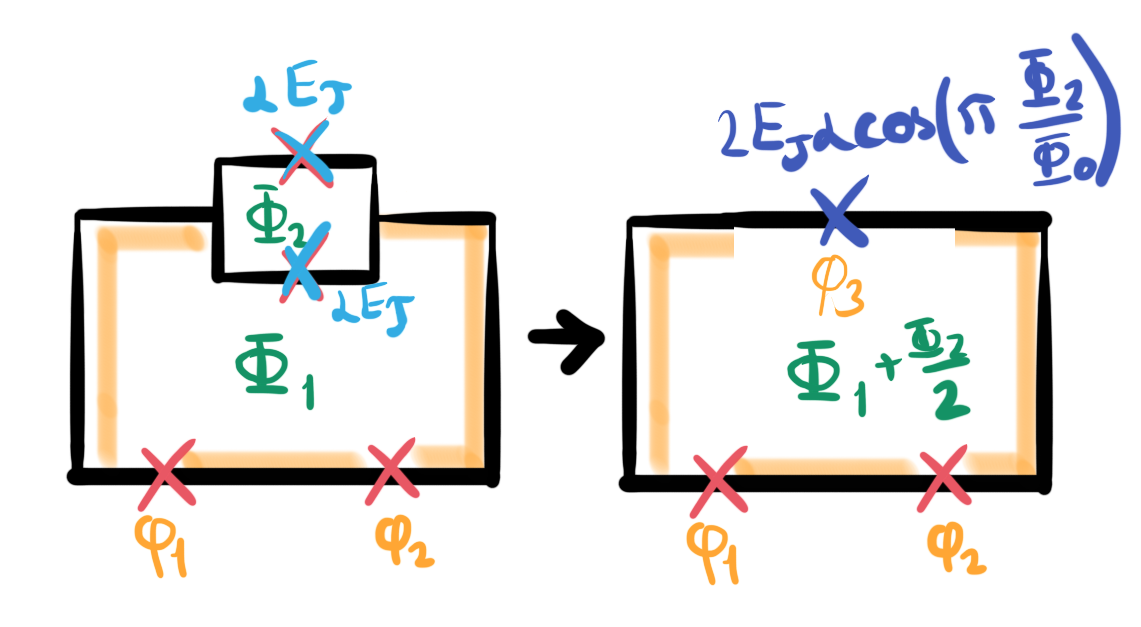
\includegraphics[height=7cm]{flux_4jj_1}
\end{figure}

\begin{enumerate}
\item   The    two   JJ's    of   SQUID    come   together    like   in
  Chapter~\ref{subsec:cpb_2} to create a single Josephson junction with
  a tuneable energy:

  \begin{equation}
    \begin{aligned}
      E_{SQUID} & = \frac{\Phi_0I_c}{2\pi}\times 2|\cos(\pi\Phi_\text{2}/\Phi_0)|\\
      & \equiv E_J \times \green{2|\cos(\pi\Phi_\text{2}/\Phi_0)|}.
    \end{aligned}
  \end{equation}

\item The effective flux penetrating the full loop is

  \begin{equation}
    \Phi_\text{total} = \Phi_1 + \frac{1}{2}\Phi_2.
  \end{equation}

  \noindent One can  think of the flux  in the SQUID loop,  $ \Phi_2 $,
  affecting the lower one only through one of the JJ.

\item    \red{\textbf{The    potential    energy}}   of    the    terms
  $ 1  - \cos(\phi_{ij}) $  of the JJ's  around the circuit  (using the
  quantisation                                                condition
  \purple{$ \phi_3  - \phi_1 +  \phi_2 -  2\pi f_\text{total} =  2\pi n
    $}):

  \begin{equation}
    U_\text{potential} = E_J \bigg[2 + 2\alpha - \cos(\phi_1) - \cos(\phi_2) - \green{2\cos(\pi f_2)}\cos\big(\purple{\phi_1 - \phi_2 + 2\pi(f_1+\frac{1}{2}f_2)}\big) \bigg].
  \end{equation}

  \noindent And this is what it looks like:
  \begin{figure}[h]
    \centering 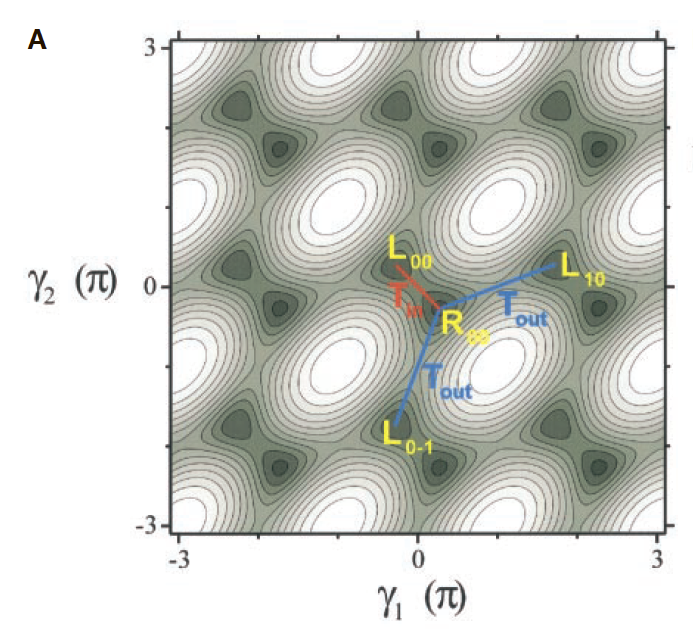
\includegraphics[height=8cm]{flux_4jj_2}
  \end{figure}

  \noindent  circulate in  the  same  direction, state  $  R  $ in  the
  opposite.   The  link  between   the  states  depends  on  parametesr
  $ \alpha $ and $ f_2 $.

\item\
  \begin{framed}\noindent
    \red{If $  f_1+\frac{1}{2}f_2 = 1  $, we recover the  3JJ potential
      from Chapter~\ref{subsec:l33jj}.}
  \end{framed}

\item \textbf{\red{The kinetic energy}} is harder to evaluate.

  \begin{equation}
    \left\lbrace \begin{aligned}
        \vec{V} & = 2eC^{-1}\vec{n}\\
        \vec{Q} & = 2e\vec{n}\\
        \red{U_{\text{kinetic}}} & \red{= \frac{1}{2}Q.V}\\
      \end{aligned}\right.  \Rightarrow \red{U_{\text{kinetic}} =
      \frac{1}{2}\left(2e\vec{n}^{\text{T}}\right)\left(2eC^{-1}\vec{n}\right)
      = \frac{(2e)^2}{2}\vec{n}^{\text{T}}C^{-1}\vec{n}},
  \end{equation}

  \noindent where $ \vec{n}  $ is the charge state on  the 3 islands in
  the  system and  $  C $  is  the capacitance  matrix  for the  system
  (confusingly, the  capacitance for  JJ's 1  and 2  is also  given the
  symbol $ C $).

  \begin{framed}\noindent
    \noindent \textbf{It is common  to work classical analogues}, where
    we would write:
    \begin{equation}
      \frac{(2e)^2}{2}\vec{n}^{\text{T}}C^{-1}\vec{n} = \frac{1}{2}\vec{p}^{T}M^{-1}\vec{p}.
    \end{equation}

    \noindent  $ M  $  is  the mass  tensor,  with nornalisation  value
    $    \hbar^2/\frac{(2e)^2}{2C}   $,    where   we    have   applied
    $ \icommutation{x}{p}=i\hbar $  and $ \icommutation{\phi}{n} =  i $ to
    generate the $ \hbar $.

  \end{framed}

\begin{framed}\noindent
  Depending on the  direction that we are looking  at tunneling across,
  we get two tensors:
  \begin{itemize}
  \item $ M_a  = \frac{1}{4}M$ for the $ \phi_1-\phi_2  = 0 $ direction
    \hfill (across the tall barrier);
  \item $  M_b =  M$ for  the $  \phi_1+\phi_2 =  0 $  direction \hfill
    (across the snall barrier);
  \end{itemize}
\end{framed}

\item  The result  it two  different transistions,  with two  different
  oscillation frequencies.

\item \red{\textbf{Make sure barrier is high enough, to localise state,
      and small enough to allow sufficient tunneling to occur.}}
\end{enumerate}
%
\newpage\section{Phase qubit. $ E_J/E_C \sim 10^6 $}
 
 \ipic{5cm}{phase_qubit}
 
 \begin{itemize}
 	\item Confined to a single potential well;
 	\item Has a bias current that controls it's state.
 \end{itemize}
 
 \newpage%
\section{Transmon source\label{sec:transmon}}

It has experimental  coherence times of $ \sim 100\,\mu  $s.  The Transmon
paper  by Sam  Bader  December  2013. There  are  two  main factors  to
consider when making a Cooper pair box
\begin{equation}\label{key}
  \mathcal{H} = E_C{\left(\hat{\red{N}}-N_\text{ext}\right)^2}- E_J\cos\left(\hat{\blue{\phi}}\right),
\end{equation}
\noindent which was discussed in Ch.~\ref{sec:cooper_pair_box}.

\begin{itemize}
\item    $   \mathbf{E_C/E_J    >>    1    }$   {High    anharmonicity,
    $  \frac{E_{12} -  E_{01}}{E_{01}}\approx -(8E_J/E_C)^{-1/2}  $, allowing
    addressation of individual transitions};
\item $ \mathbf{E_C/E_J  <<1 }$ {Low charge noise  sensitivity, so that
    $  N_\text{ext} $  does not  jump and  affect the  quadratic energy
    dependance};
\end{itemize}

\noindent    \red{\textbf{It     is    usually    better     to    have
    $ \mathbf{E_C/E_J  <<1 }$, because anharmonicity  decreases slowly,
    while the charge sensitivity will greatly improve.}} To do this, we
need to increase the apparent capacitance  of the junction with a large
shunt capacitance:

\begin{figure}[h]
  \centering 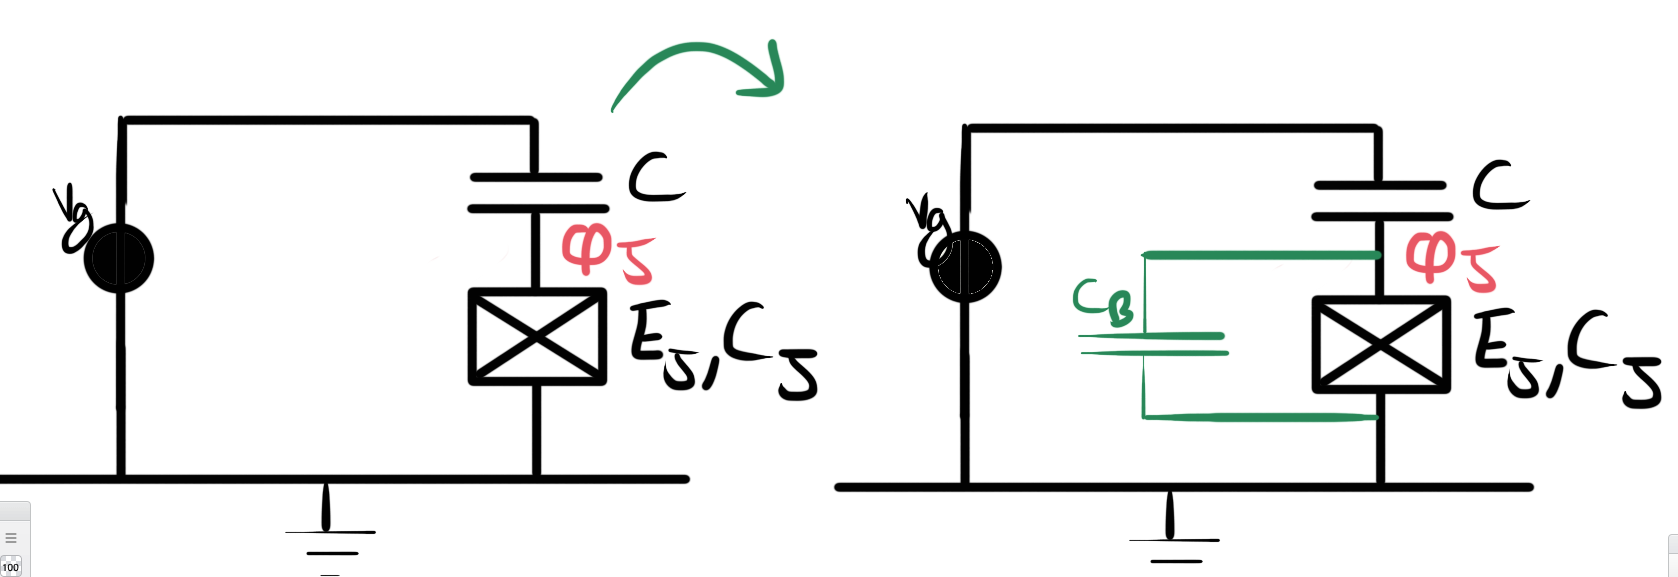
\includegraphics[height=4cm]{transmon_1}
\end{figure}

\noindent

\begin{framed}\noindent
  The same  equations are used as  for the Cooper pair  box, except the
  capacitance $ C_J \rightarrow C_B$, which is magnitudes larger.
  \begin{equation}\label{key}
    \mathcal{H}_\text{transmon} = E_C{\left(\hat{\red{N}}-N_\text{ext}\right)^2}- E_J\cos\left(\hat{\blue{\phi}}\right),
  \end{equation}

\end{framed}

\newpage
%
% -*- TeX-master: "all_the_notes.tex" -*-

\section{Transmission       line       and       resonator       from
  circuits}\label{sec:transmission-line}

We treat the transmission line as a chain of inductors and capacitors
and  that is  lossless (i.e  $ R=0  $ and  $ G=0  $ =  no conductance
between the lines) with

  \begin{equation}
    l \approx \mu_0 \text{ - the inductance per unit length}\qquad c \approx \epsilon_0 \text{ - the capacitance per unit length},
  \end{equation}

  \noindent  as shown  in  Fig.\ref{transtLine}.  Recall  that for  a
  device   of    size   $    \alpha   $,    the   capacitance    will   be
  $ C \approx \epsilon_0\alpha $.  The  current and the voltage in the line
  will have components going in opposite directions

  \begin{equation}
    \label{tlineCurrentVoltage}
    \mathbf{V_{\pm} = V_0e^{\pm ikx-i\omega t};\qquad I_{\pm} = I_0e^{\pm ikx-i\omega t}},
  \end{equation}

  \noindent and be  related to each other via  the complex impedance.
  (\textbf{Impedance} is equivalent to \textbf{Resistance} but for an
  AC circuit,  where charge  buildup and  current through  coils will
  create time-varying emf in the circuit)

 \begin{equation}
   V_{\pm}= \pm ZI_{\pm}
 \end{equation}

 \begin{figure}[h]
   \caption{Treat the transmission  line as a chain  of inductors and
     capacitors and that is lossless \label{transtLine}}
   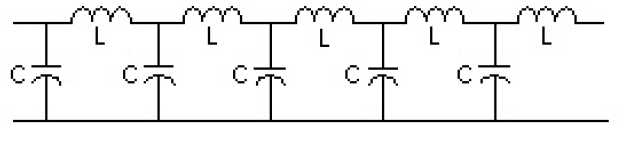
\includegraphics[height=3cm]{tline}
 \end{figure}

 \noindent  We write  the  following equations  from their  classical
 analogues

 \begin{equation}
   \left\lbrace \begin{aligned}
       V & = -\frac{d\Phi}{dt} = -L\frac{dI}{dt}\\
       I & = -\frac{dQ}{dt} = -C\frac{dV}{dt}
     \end{aligned}\right.\Rightarrow \text{ per unt length} \Rightarrow
   \left\lbrace \begin{aligned}
       \frac{dV}{dx} & = - l\frac{dI}{dt}\\
       \frac{dI}{dx} & - c\frac{dV}{dt},
     \end{aligned}\right.
   \label{tlineDiff}
 \end{equation}

 \begin{itemize}
 \item    We     substitute    Eq.\eqref{tlineCurrentVoltage}    into
   Eq.\eqref{tlineDiff} to get

  \begin{equation}
    \left\lbrace \begin{aligned}
        ikV_0&=i\omega lI_0\\
        -i\omega I_0 & = -ickV_0
      \end{aligned}\right. \Rightarrow\left\lbrace \begin{aligned}
        Z_0&=\frac{V_0}{I_0} = \frac{\omega l }{k}\\
        Z_0&=\frac{V_0}{I_0} = \frac{k}{\omega c}\\
      \end{aligned}\right.  \Rightarrow \red{\mathbf{Z_0 =
        \sqrt{\frac{l}{c}}}}\approx
    100\Omega
  \end{equation}

\item We differentiate Eq.\eqref{tlineDiff}

  \begin{equation}
    \frac{d^2V}{dx^2} = -l\frac{d^2I}{dt\partial x} = -l\bigg(-c\frac{d^2V}{dt^2}\bigg) \Rightarrow V_{xx} = \frac{1}{1/lc}V_{tt},
  \end{equation}

  \noindent  which has  the  exact  same form  as  the wave  equation
  $ y_{xx}=\frac{1}{v^2}y_{tt} $, from which one can get the speed of
  wave propagation

  \begin{equation}
    \red{v=\frac{1}{\sqrt{lc}}}
  \end{equation}
\end{itemize}

\begin{figure}[h]
  \centering%
  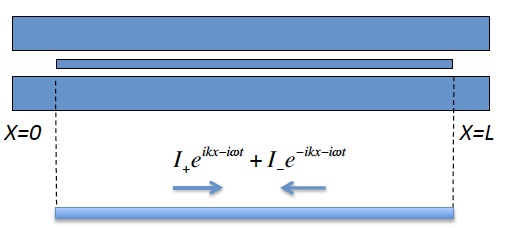
\includegraphics[height=4cm]{res1}%
  \caption{\label{tlineres1}}
\end{figure}

So  far   we  have   had  a  transmission   line  with   no  boundary
conditions. But now  lets us look at a resonator,  depicted in figure
which has two ends which are cut off and at which

\begin{itemize}
\item  \textbf{The current  $ I=0  $}: no  charge may  flow at  these
  points of cut.
\end{itemize}

Mathematically speaking

 \begin{equation}
   \left\lbrace \begin{aligned}
       I(x=0) & = I_{+}(x=0)+I_-(x=0)=0\\
       I(x=L) & = I_{+}(x=L)+I_-(x=L)=0
     \end{aligned}\Rightarrow\begin{aligned}
       \red{I_+}&\red{=-I_-}\\
       I_+&= -I_-e^{-i2kL}
     \end{aligned} \Rightarrow \red{k=\frac{\pi n}{L}}, \right.
 \end{equation}

 \noindent and the  total current at any point in  the resonator will
 be a point on a standing wave

 \begin{equation}
   I(x,t) = I_+(x,t) + I_-(x,t) = I_+e^{i\frac{\pi n}{L}x-i\omega t} - I_+e^{-i\frac{\pi n}{L}x-i\omega t} = {{I_0\sin\bigg[\frac{\pi n}{L}x\bigg]e^{-i\omega t}}}.
   \label{tlineCurrent}
 \end{equation}

 \noindent  Evaluating  the  voltage using  Eq.\eqref{tlineDiff}  and
 Eq.\eqref{tlineCurrent}

 \begin{equation}
   \begin{aligned}
     \frac{dI}{dx} &= - c\frac{dV}{dt}\\
     kI_0\cos(kx)e^{-i\omega t}& =-c\frac{dV}{dt}\\
     \frac{-1}{i\omega}kI_0\cos(kx)e^{-i\omega t}& =-cV\\
     & \Rightarrow\qquad V &=  -i\frac{k}{\omega c}I_0\cos(kx)e^{-i\omega t}\\
     &&=|Z|I_0\cos(kx)e^{-i\omega t}e^{-i\pi/2}\\
     &&=V_0\cos \bigg(\frac{\pi n}{L}x\bigg)\exp\bigg[-i\omega t-i\pi/2\bigg]\\
   \end{aligned}
 \end{equation}

 \noindent or fully the result is (and depicted in Fig.\ref{tlineVI})

 \red{ \begin{equation}
     \begin{aligned}
       V & =V_0\cos \bigg(\frac{\pi n}{L}x\bigg)\exp\bigg[-i\omega t-i\frac{\pi}{2}\bigg]\\
       I & =I_0\sin \bigg(\frac{\pi n}{L}x\bigg)\exp\bigg[-i\omega t\bigg]\\
       V_0&=|Z|I_0
     \end{aligned}
   \end{equation}}

 \begin{figure}
   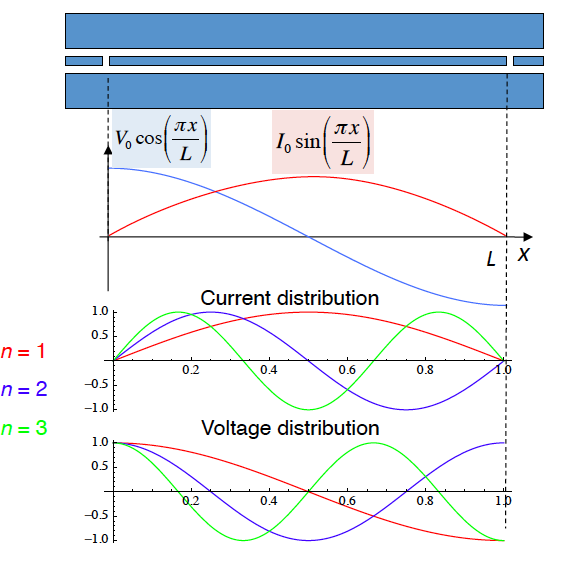
\includegraphics[height=7cm]{vires}
   \caption{Voltage has an anti-node at  the two sides, while current
     has  a  node.    Multiple  modes  can  be   accomodated  by  the
     resonator\label{tlineVI}}
 \end{figure}

 \subsection{The voltages at the gaps of the resonator}
 Now when we consider a boundary,  we shall label + as moving towards
 a boundary, and - as moving  away.  By defining the transmission and
 reflection as

 \begin{equation}
   t=\frac{|V_{R}^{-}|}{|V_{L}^{+}|};\quad r=\frac{|V_{L}^{-}|}{|V_{L}^{+}|};\quad t=1+r,
 \end{equation}

 \noindent we shall write the propagating waves as follows

 \begin{align}
   V_L^{+} & = V_0e^{ikx-i\omega t}\\
   V_L^{-} & = rV_0e^{\red{-}ikx-i\omega t}\\
   V_R^{+} & = tV_0e^{ikx-i\omega t},
 \end{align}

 \noindent where  we assume that no  wave is incident from  the right
 hand  side ($  V_R^{+}=0  $).   Recalling Eq.\eqref{tlineDiff}  that
 relates the  current to the voltage  in a line, let  us evaluate the
 current corresponding to each voltage component in the table below

 \setlength{\extrarowheight}{3mm}
 \begin{table}[h]
   \caption{In               the              last               step
     $     \mathbf{I_0}=V_0\frac{k}{\omega    l}=V_0\frac{1}{v     l}    =
     V_0\frac{\sqrt{lc}}{l} = V_0\sqrt{\frac{c}{l}}=V_0/Z_0 $.}
   \hspace*{-2.5cm}
   \begin{tabular}{|c|c|c|c|c|c|c|c|}
     \hline
     \textbf{Component} & {Voltage}, $ V $ & \multirow{4}{1.5ex}{$ \Rightarrow $}& $ \frac{dV}{dx} \equiv -l\frac{dI}{dt}$ &\multirow{4}{1.5ex}{$ \Rightarrow $}&  $ \frac{dI}{dt} $ &\multirow{4}{1.5ex}{$ \Rightarrow $}&  Current $ I $ \\\cline{1-2}\cline{4-4}\cline{6-6}\cline{8-8}
     $ \text{Left}\ + $ & $ \mathbf{V_0e^{ikx-i\omega t}} $ & & $ ikV_0e^{ikx-i\omega t} $ && $ -\frac{ik}{l}V_0e^{ikx-i\omega t} $ && $ \frac{k}{\omega l}V_0e^{ikx-i\omega t}  = \mathbf{I_0e^{ikx-i\omega t}}$\\\cline{1-2}\cline{4-4}\cline{6-6}\cline{8-8}
     $ \text{Left}\ - $ & $ \mathbf{rV_0e^{\red{-}ikx-i\omega t}} $ & & $ -ikrV_0e^{\red{-}ikx-i\omega t} $ && $ \frac{ik}{l}rV_0e^{\red{-}ikx-i\omega t} $ && $ -\frac{k}{\omega l}rV_0e^{\red{-}ikx-i\omega t}  = \mathbf{-rI_0e^{\red{-}ikx-i\omega t}}$\\\cline{1-2}\cline{4-4}\cline{6-6}\cline{8-8}
     $ \text{Right}\ + $ & $\mathbf{ tV_0e^{ikx-i\omega t}} $ & & $ iktV_0e^{ikx-i\omega t} $ && $ \frac{ik}{l}tV_0e^{ikx-i\omega t} $ && $ \frac{k}{\omega l}tV_0e^{ikx-i\omega t}  = \mathbf{tI_0e^{ikx-i\omega t}}$\\\hline
   \end{tabular}
 \end{table}

 \newpage
 Now, the equality  of the currents and voltages on  the two sides of
 the  gap  at  $  x=0  $  \red{\textbf{and  including  the  potential
     difference         drop          across         the         gap,
     $      V_{\text{drop}}      =     I_{R}^{+}Z_{\text{gap}}      =
     \frac{tI_0e^{-i\omega t}}{i\omega C_{\text{gap}}} $, that causes
     the current on the other side of the gap}}

 \begin{equation}
   \left\lbrace\begin{aligned}
       I_0 e^{-i\omega t}-rI_0e^{-i\omega t} & = tI_0e^{-i\omega t}\\
       V_0 e^{-i\omega t}+rV_0e^{-i\omega t} & = tV_0e^{-i\omega t}+\frac{tI_0}{i\omega C_\text{gap}}\\
     \end{aligned}\right.\Rightarrow
   \left\lbrace\begin{aligned}
       1-r & =t\\
       1+r & = \bigg(1+\frac{1}{i\omega C_{\text{gap}}Z}\bigg)t
     \end{aligned}\right.
 \end{equation}

 \noindent and one can simply solve for $ r $ and $ t $ coefficients

 \begin{equation}\label{tLinert}
   \mathbf{\red{t= \frac{1}{1+\frac{1}{i2\omega C_\text{gap}Z}} = \frac{i\alpha}{1+i\alpha};\quad	 r = \frac{1}{1+i\alpha};\quad \alpha = 2\omega C_\text{gap}Z.}}
 \end{equation}

 \begin{figure}
   \centering%
   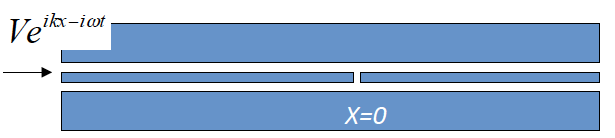
\includegraphics[height=3cm]{gap}
 \end{figure}

 Now suppose that  we defined another gap further down  the line. Let
 us see what the  resulting voltage at $ x=L $  would be. The voltage
 that is transmitted across the gap initially is $ tV_0 $

 \begin{multline}\label{tlineMUltiple}
   tV_0 \rightarrow \left\lbrace \text{travels $ L $ to
       $    x=L    $}\right\rbrace    \rightarrow   tV_0e^{ikL-i\omega    t}    \\
   \rightarrow\left\lbrace \text{reflects, travels $ L  $ to $ x=0 $,
       reflects,  travels  L  to $  x=L  $  }\right\rbrace\rightarrow
   r^2tV_0e^{ik3L-i\omega         t}\\        \rightarrow\left\lbrace
     \text{reflects, travels $ L $ to $ x=0 $, reflects, travels L to
       $ x=L $
     }\right\rbrace\rightarrow     r^4tV_0e^{ik5L-i\omega      t}     \\
   \rightarrow\left\lbrace \text{reflects, travels $ L  $ to $ x=0 $,
       reflects,  travels  L  to $  x=L  $  }\right\rbrace\rightarrow
   r^6tV_0e^{ik7L-i\omega t} \\ \rightarrow\cdots
 \end{multline}

 \noindent so that the total voltage

 \begin{equation}\label{tlineTotalVoltage}
   \begin{aligned}
     V(x=L) & = tV_0e^{ikL-i\omega t}\bigg(1+r^2e^{i2kL}+r^4e^{i4kL}+r^6e^{i6kL}+\cdots\bigg)\\
     & = tV_0e^{ikL-i\omega t}\sum_{n=0}^{\infty}\bigg(r^2e^{2ikL}\bigg)^n, \quad\text{and since $ r<1 $ this is a convergent power series}\\
     & = \mathbf{\frac{tV_0e^{ikL-i\omega t}}{1-r^2e^{2ikL}}.}
   \end{aligned}
 \end{equation}

 \noindent To make good use of this, we need to use

 \begin{equation}\label{tlineApprox}
   \left\lbrace
     \begin{aligned}
       e^{i\alpha+i\alpha^2/2} & = 1+i\alpha +O(\alpha^3) \text{ (proof by simple expansion)}\\
       r & = (1+i\alpha)^{-1} \text{ (from before)}
     \end{aligned}\right.\Rightarrow r^2 \approx e^{-i2\alpha
     +\alpha^2}
 \end{equation}

 \noindent \red{This and further mathematical  stuff will lead to the
   voltage inside the resonator to be}

 \begin{equation}\label{tlineVoltage}
   V_r = \frac{V_0}{\alpha}\frac{i(-1)^{n}e^{-i\omega t}}{1+i\frac{2\delta\omega}{\Delta\omega}};\quad \Delta\omega = 2\alpha^2f_0;\quad \delta\omega = \text{ offset from $ n^{th} $ resonance}.
 \end{equation}

 \noindent  \red{As  can be  seen,  the  maximum voltage  inside  the
   resonator is $  1/\alpha $ times larger than the  external field -
   we  have  boosted   the  total  field  from   the  combination  of
   reflections.}   In a  similar  way the  voltage/power leaving  the
 resonator are

 \begin{equation}\label{tlineLeaving}
   V_{out} = tV_r = \frac{V_0}{\alpha}\frac{i(-1)^{n+1}e^{-i\omega t}}{1+i\frac{2\delta\omega}{\Delta\omega}}; \quad P_{out} = \frac{P_0}{1+\left(\frac{2\delta\omega}{\Delta\omega}\right)^2}.
 \end{equation}

  \begin{figure}[h]
    \centering%
    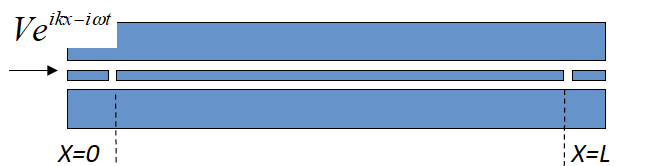
\includegraphics[height=3cm]{gap1}
  \end{figure}


  \red{Important is the quality factor of the resonator.  This is the
    ratio of  the resonance frequency  to the width of  the resonance
    peak}

  \red{\begin{equation}\label{key}                 Q                =
      \frac{\omega_{\text{resonance}}}{\Delta\omega}=\frac{\pi}{\left(2\omega
          ZC_{gap}\right)^2}.
    \end{equation}}

   \begin{figure}[h]
     \centering%
     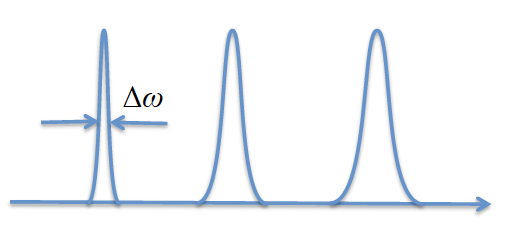
\includegraphics[height=3cm]{res}
   \end{figure}

   Using     results     of     Table.\ref{tab:conversion2},     with
   $      V      =     V_0\bigg(a+a^\dagger\bigg);\quad      I      =
   iI_0\bigg(a-a^\dagger\bigg) $, and the  results from the classical
   resonator
   $ V=V_0\cos(\frac{\pi n}{L}x);\quad I=I_0\sin(\frac{\pi n}{L}x) $, the
   quantum field is

   \begin{align}
     \hat{V} & = \sqrt{\frac{\hbar\omega}{2c}}\bigg(a+a^\dagger\bigg)\cos(\frac{\pi n}{L}x)\\
     \hat{I} & = i\sqrt{\frac{\hbar\omega}{2l}}\bigg(a-a^\dagger\bigg)\sin(\frac{\pi n}{L}x)\\
   \end{align}

   \noindent and the total energy, given by the Hamiltonian is

   \begin{equation}\label{tlineTOtalGamil}
     \begin{aligned}
       \mathcal{H} & = \frac{1}{L}\int_{0}^{L}\bigg(\frac{l\hat{I}^2}{2}+\frac{c\hat{V}^2}{2}\bigg)dx \\
       & = \frac{l}{2}\frac{-\hbar\omega}{2l}\bigg(a-a^{\dagger}\bigg)^2\frac{1}{L}\int_{0}^{L}\cos^2(\frac{\pi n}{L}x)dx + \frac{c}{2}\frac{\hbar\omega}{2c}\bigg(a+a^{\dagger}\bigg)^2\frac{1}{L}\int_{0}^{L}\sin^2(\frac{\pi n}{L}x)dx\\
       & = -\frac{\hbar\omega}{4}\frac{1}{2}\bigg(aa-aa^{\dagger}-a^{\dagger}a+a^{\dagger}a^{\dagger}\bigg)+\frac{\hbar\omega}{4}\frac{1}{2}\bigg(aa+aa^{\dagger}+a^{\dagger}a+a^{\dagger}a^{\dagger}\bigg)\\
       &       =      \frac{\hbar\omega}{8}\bigg(aa^{\dagger}+a^{\dagger}a\bigg)=
       \frac{\hbar\omega}{8}\bigg((a^{\dagger}a+1)+a^{\dagger}a\bigg)=\mathbf{\hbar\omega\bigg(\hat{N}+\frac{1}{2}\bigg)},
     \end{aligned}
   \end{equation}

   \noindent so the resonator is a quantum harmonic oscillator.

   \subsection{Resonator types}
   \label{sec:resonator-types}

   \begin{itemize}
   \item  $\lambda/2$  resonator  -   transmission  lines  at  either
     end. Transmission is maximum;
   \item  $\lambda/4$  resonator -  one  end  is grounded,  other  is
     coupled to transmission line. Transmission has a dip.
   \end{itemize}

   \subsection{Resonator Emission}
   \label{sec:resonator-emission}

   This is based off a slightly related paper \cite{Galli_2009} which
   talks about shining a light on a cavity. In general, the intensity
   of a signal from a resonator can be fitted by:

   \begin{framed}\noindent
     \begin{equation}
       \text{Intensity} = I_0 + I_1 \frac{\left[ q + 2(\omega - \omega_{0})/\Gamma \right]^2}{1 + \left[ 2(\omega - \omega_0)/\Gamma \right]^2}
     \end{equation}

     \noindent where apart  from scaling and offset  $I_0, I_1$ there
     is:
     \begin{itemize}
     \item
       $q          =         \frac{\text{Resonant          scattering
           amplitude}}{\text{Non-resonant amplitude}}$;
     \item $\Gamma$ is the FWHM of the scattering (linewidth)
     \end{itemize}
   \end{framed}

   \noindent  Light shone  on the  cavity in  \autoref{fig:gali_2009}
   will be reflected in one of two regimes
   \begin{itemize}
   \item Emission at the cavity  frequency and inevitable emission to
     continuum    (non-resonant)    frequency   \hfill    $q\approx1$
     \autoref{fig:gali_2009}a - asymmetric fit;
   \item   Non-resonant  emission   at  a   continuum  of   available
     frequencies \hfill  $q << 0$ \autoref{fig:gali_2009}b  - flipped
     lorentzian;
   \item (Not  observed -  very strong  resonant emission  - standard
     lorentzian) \hfill $q >> 1$.
   \end{itemize}

     \begin{figure}[h]
       \centering \includegraphics[height=6cm]{gali_2009}
       \caption{\small Bigger area of  reflect light means that there
         is       more      contribution       from      non-resonant
         processes. \textbf{Note that in  figure B, the lorenztian is
           flipped  by  the experiment  (from  formula  is should  be
           upside down).}\label{fig:gali_2009}}
     \end{figure}

\begin{figure}[h]
  \centering
  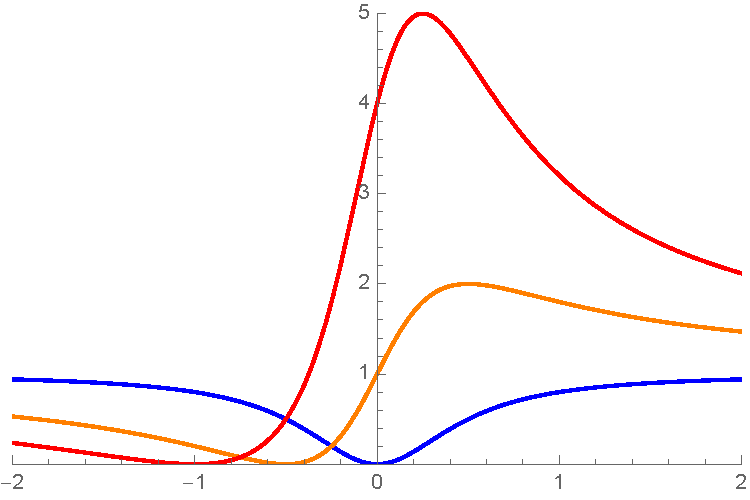
\includegraphics[height=5cm]{mathematica/fano_simulation}
  \caption{\small   Red:   $q=2$,   Orange:   $q=1$,   Blue:   $q=0$.
    \textbf{Note that when  there is very weak  resonant emission, we
      are centred on the dip, \red{otherwise the dip will actually be
        off-center}}.\label{fig:fano_simulation}}
\end{figure}

\newpage
%
% -*- TeX-master: "../all_the_notes.tex" -*-

\section{Qubit-Resonator System \cite{cqeResonator}}
\begin{enumerate}
\item  The two-level  qubit with  a separation  between the
  energy levels $ \Delta E $ has the Hamiltonian

\begin{equation}
  \mathcal{H}_{a}= -\frac{\Delta E}{2}\sigma_z.
  \label{qrA}
\end{equation}

\item  This qubit  is  placed  in close  proximi  y with  a
  resonator,  which,  as  we  have  seen  in  the  previous
  chapter, has a harmonic oscillator-like Hamiltonian

\begin{equation}
  \mathcal{H}_{r}={\hbar\omega}\bigg(\red{\hat{N}}+\frac{1}{2}\bigg)\qquad \qquad a^{\dagger}\ket{N}=\sqrt{N+1}\ket{N+1}; \qquad a\ket{N}=\sqrt{N}\ket{N=1}.
  \label{qrR}
\end{equation}

\noindent  where for  simplicity  we  neglect the  constant
energy term.

\item The general state of a  system, where the qubit is in
  state $ n $ and the resonator in state $ N $ (i.e.  $ N $
  photons) will be

\begin{equation}
  \ket{n,N}.
\end{equation}

\noindent  Qualitatively   speaking,  the  way   the  qubit
interacts with the resonator in one of the two ways

\begin{itemize}
\item Qubit absorbs a photon and transitions to the excited
  state: $ \blue{\ket{0,N+1} \rightarrow \ket{1,N}} $;
\item Qubit relaxes  to ground state and  releases a photon
  into the resonator: $ \red{\ket{1,N} \rightarrow \ket{0,N+1}} $.
\end{itemize}

This can be expressed via the interaction Hamiltonian

\begin{equation}
  \mathcal{H}_{\text{int}}=\blue{a\sigma^+}+\red{a^{\dagger}\sigma^-}.
  \label{qrInt}
\end{equation}
\end{enumerate}
Giving in total \iframe{\LARGE
  \[ \mathcal{H}  =\blue{-\frac{\Delta E}{2}\sigma_z}+\blue{{\hbar\omega_r}a^\dagger
      a} + \red{g_0\bigg({a\sigma^+}+{a^{\dagger}\sigma^-}\bigg)},
  \]}

\ipicCaption{8cm}{cavityPic1}{Interaction   between  states
  with  same energy  creates the  superposed states  in the
  middle. \label{qb_res_ladder}}
  
\noindent  This gives  rise  to energy  levels depicted  in
Fig.\ref{qb_res_ladder} which we write  out in terms of the
basis           states,            recalling           that
$               \sigma_z=\iupKetBra-              \idownKetBra$,
$\sigma^+=\ketbra{\uparrow}{\downarrow}$,
$\sigma^-=\ketbra{\downarrow}{\uparrow}$,
$       a        =       \sqrt{N+1}\ketbra{N}{N+1}       $,
$ a^\dagger = \sqrt{N+1}\ketbra{N+1}{N} $:

\begin{equation}
  \begin{aligned}
    \mathcal{H} & = \blue{\bigg[\frac{\Delta E}{2}\big(\iupKetBra-\idownKetBra\big)\bigg]\otimes\mathbb{I}_{N}} + \blue{\mathbb{I}_{n}\otimes\bigg[\hbar\omega_r\sum_{N}N\ketbra{N}{N}\bigg]} +\\
    &\ +  \red{g_0\bigg[\ketbra{\uparrow}{\downarrow}\sqrt{N+1}\sum_{N}\ketbra{N}{N+1}+\ketbra{\downarrow}{\uparrow}\sum_{N}\sqrt{N+1}\ketbra{N+1}{N}\bigg]}\\
    & = \sum_{N}\quad\blue{\bigg(\hbar N\omega_r-\frac{\Delta E}{2}\bigg)\ketbra{\downarrow,N}{\downarrow,N}+\bigg(\hbar N\omega_r+\frac{\Delta E}{2}\bigg)\ketbra{\uparrow,N}{\uparrow,N} \leftarrow \text{ diagonal }}\\
    &\ +  \red{g_0\sqrt{N+1}\bigg[\ketbra{\uparrow,N}{\downarrow,N+1}+\ketbra{\downarrow,N+1}{\uparrow,N}\bigg] \leftarrow \text{ cross terms }}\\
  \end{aligned}
\end{equation}

\noindent and in matrix form

\begin{equation}\label{eqn:qubitCavityHamil}
  \mathcal{H} = \kbordermatrix{
    & \ket{\downarrow,N} & \ket{\uparrow,N} & \ket{\downarrow,N+1} & \ket{\uparrow,N+1} \\
    \bra{\downarrow,N} &\blue{\hbar N\omega_r-\frac{\Delta E}{2}} & 0 & 0 & 0\\
    \bra{\uparrow,N} & 0 & \blue{\hbar N\omega_r+\frac{\Delta E}{2}} & \red{g_0
      \sqrt{N+1}} & 0\\
    \bra{\downarrow,N+1} & 0 & \red{g_0\sqrt{N+1}} & \blue{\hbar (N+1)\omega_r-\frac{\Delta E}{2}} & 0\\
    \bra{\uparrow,N+1} & 0 & 0 & 0 & \blue{\hbar (N+1)\omega_r+\frac{\Delta E}{2}}.\\
  }
\end{equation}

\subsection{General solutions}
\begin{enumerate}
\item For the ground state, we take the top row, which will
  have the lowest energy
  \[
    \iket{\downarrow,0} = \begin{pmatrix} 1 \\0\\0\\\vdots
    \end{pmatrix}\text{ with energy }
    -\frac{\Delta E}{2}.
  \]
 	
\item  Then diagonalising  an  arbitrary  middle matrix  (N
  value incremented for convenience)
 	
 	\begin{equation}\begin{aligned}
            \mathcal{H}_{\text{middle}}
            & = \kbordermatrix{&\ket{\uparrow,N} & \ket{\downarrow,N+1}\\
              \bra{\uparrow,N} & \blue{\hbar\omega_r(N+\frac{1}{2}) + \hbar\Delta} & \red{g_0\sqrt{N+1}}\\
              \bra{\downarrow,N+1} & \red{g_0\sqrt{N+1}} & \blue{\hbar\omega_r(N+\frac{1}{2}) - \hbar\Delta}}\\
            &= \blue{\hbar\omega_r(N+\frac{1}{2})\mathbb{I} +\frac{ \hbar\Delta}{2}\sigma_z} + \red{g_0\sqrt{N+1}\sigma_x}\\
            & = \blue{\hbar\omega_r(N+\frac{1}{2})\mathbb{I}} + \frac{1}{2}\sqrt{(\hbar\Delta)^2 + 4g_0^2(N+1)} \bigg(\cos(\theta)\sigma_z + \sin(\theta)\sigma_x\bigg)\\
            & = \hbar\omega_r(N+\frac{1}{2})\mathbb{I} + E_{\text{coupled}}(\cos(\theta)\sigma_z + \sin(\theta)\sigma_x)\\
            &    \text{where     }    E_\text{coupled}    =
            \frac{\hbar}{2}\sqrt{\Delta^2    +    4(g_0/\hbar)^2(N+1)};\qquad
            \tan(\theta) = \frac{g_0\sqrt{N+1}}{\hbar\Delta/2}.
          \end{aligned}
 	\end{equation}
 	
      \item  {   \noindent  By   applying  a   rotation  of
          $ \theta/2 $ about the y-axis
 		
 		\[
                  U                                       =
                  \exp\big[i\frac{\theta}{2}\sigma_y\big] =
                  \cos(\theta/2)\mathbb{I}                +
                  i\sin(\theta/2)\sigma_y,
 		\]}
 	
              \noindent    we    will     end    up    with
              \iframe{\[           \mathcal{H'}           =
                  \hbar\omega_r(N+\frac{1}{2})\mathbb{I}  +
                  \frac{E_\text{coupled}}{2}\sigma_z
                  =                         \begin{pmatrix}
                    \hbar\omega_r(N+\frac{1}{2})          +
                    \frac{E_\text{coupled}}{2}    &   0\\0&
                    \hbar\omega_r(N+\frac{1}{2})          -
                    \frac{E_\text{coupled}}{2}
                  \end{pmatrix}
                \]
                \begin{itemize}
 		\item           \textbf{Eigenstates}:\hfill
                  \iket{\tilde{0}}, \iket{\tilde{1}};
 		\item     \textbf{Eigenenergies}:    \hfill
                  $     \hbar\omega_r(N+\frac{1}{2})    \pm
                  \frac{E_\text{coupled}}{2} $.
                \end{itemize}
              }
 	
            \item In the  original basis of \iket{\uparrow,
                N}, \iket{\downarrow, N} \iframe{
 		\begin{itemize}
                \item \textbf{Eigenstates:}
                  \[
                    \begin{aligned}
                      \iket{+,N}             &            =
                      U^{\dagger}\ket{\tilde{1}}          =
                      \bigg(\cos(\theta/2)\mathbb{I}-i\sin(\theta/2)\sigma_y\bigg)
                      \begin{pmatrix}1\\0 \end{pmatrix} =
                      \begin{pmatrix} \cos(\theta/2)\\\sin(\theta/2)\end{pmatrix} \\
                      \iket{-,N}             &            =
                      U^{\dagger}\ket{\tilde{0}}
                      =                     \begin{pmatrix}
                        -\sin(\theta/2)\\\cos(\theta/2)
                      \end{pmatrix} \equiv -\sin(\theta/2)\iket{\uparrow,N} + \cos(\theta/2)\iket{\downarrow,N+1}\\
                    \end{aligned}
                  \]
 		\item     \textbf{Eigenenergies:}    \hfill
                  $         \text{Energies}_{\pm}         =
                  \hbar\omega_r(N+\frac{1}{2})          \pm
                  \frac{E_\text{coupled}}{2} $
                \end{itemize}
              }
            \end{enumerate}
 
            \ipic{5cm}{cavityPic2}
 
            \noindent  The  eingenstate   spectrum  of  the
            \iket{\pm,N}  states  is  ladder-like.   For  a
            single photon, and on resonance, $ \Delta = 0 $
            the entangled states are
 
 \[
   \iket{\pm,1}      =     \frac{\iket{\uparrow,0}      \pm
     \iket{\downarrow,1}}{\sqrt{2}}   \quad   \text{   with
     energies     }    \hbar\omega_r(N+\frac{1}{2})     \pm
   g_0\sqrt{N+1},
 \]
 
 \noindent will flip flop  between the original levels with
 a Rabi frequnecy $ 2g_0/2\pi $. As the atom is excited for
 exactly half of the state, with  a decay rate $ \gamma $ ,
 and the cavity is excited for the other half of the state,
 with  a decay  rate  $  \kappa $  the  net  decay rate  is
 $   \frac{\gamma+\kappa}{2}   $   and  to   observe   Rabi
 oscillations between the original states
 
 \[
   2g  > \frac{\kappa+\gamma}{2}  \qquad\qquad\text{\red{to
       see Rabi oscillation  before decay == \textbf{strong
         coupling}}}
 \]
 
 \subsection{Resonant case = Dressed States} {\LARGE
   \[\hbar\omega_r \equiv \Delta E\]}
 \begin{equation}
   \mathcal{H} = \kbordermatrix{
     & \ket{0,N-1} & \ket{1,N-1} & \ket{0,N} & \ket{1,N} \\
     \bra{0,N-1} &\blue{\Delta E\big(N-\frac{3}{2}\big)} & 0 & 0 & 0\\
     \bra{1,N-1} & 0 & \blue{\Delta E\big(N-\frac{1}{2}\big)} & \red{g_0\sqrt{N}} & 0\\
     \bra{0,N} & 0 & \red{g_0\sqrt{N}} & \blue{\Delta E\big(N-\frac{1}{2}\big)} & 0\\
     \bra{1,N} & 0 & 0 & 0 & \blue{\Delta E\big(N+\frac{1}{2}\big)}\\
   },
 \end{equation}

 \noindent and a degeneracy  appears between the two middle
 states  as in  Fig.\ref{qrLevel}. The  middle part  of the
 Hamiltonian is treated as a two levels system

\begin{equation}
  \mathcal{H}_{\text{middle}} = \begin{pmatrix}
    \blue{\Delta E\big(N-\frac{1}{2}\big)} & \red{g_0\sqrt{N}}\\
    \red{g_0\sqrt{N}} & \blue{\Delta E\big(N-\frac{1}{2}\big)}
  \end{pmatrix}\qquad\Rightarrow\qquad\kbordermatrix{
    &\ket{1,N-1}&\ket{0,N}\\
    \bra{1,N-1}& 0 & \red{g_0\sqrt{N}}\\
    \bra{0,N}& \red{g_0\sqrt{N}} & 0},
\end{equation}

\noindent  which  can  be   diagonalised  with  two  states
separated by  an energy $  g_0\sqrt{N} $, also  depicted in
Fig.\ref{qrLevel}.   The  degeneracy  is lifted  for  every
single state, and these states are known as dressed.

\begin{equation}
  \ket{\Psi} = \frac{\ket{0,N}\pm\ket{1,N-1}}{\sqrt{2}} \qquad E = \pm{g_0\sqrt{N}}.
\end{equation}

\begin{figure}
  \ipic{6cm}{qrLevel}
  \caption{Degeneracy     between      different     photon
    states  \label{qrLevel}.  Note  that  relative to  zero
    energy  (for   $  \ket{0,0}   $)  one  is   shifted  by
    $ N\hbar\omega_r-\frac{\Delta E}{2}=\bigg(N-\frac{1}{2}\bigg)\Delta E $}
\end{figure}

Fig.\ref{qrDresssed} is intepreted as follows:

\begin{itemize}
\item We have a qubit, that  is either in state \iket{0} or
  \iket{1},  whose energy  spectrum is  shown by  the green
  lines.  By  controlling some  bias e.g. gate  voltage, we
  choose  the energy  difference $  \Delta E  $ between  the two
  levels.
\item  We   apply  a  \textbf{fixed}  resonator   drive  at
  $  \hbar\omega_r $.   This  makes  a copy  of  the original  qubit
  states,  shifted   by  $  \hbar\omega_r  $.    This  configuration
  corresponds  to  the  \blue{blue}   terms  in  the  above
  equations.
\item At  the degeneracy point for  the new qubit-resonator
  system, degeneracy will be  lifted by the qubit-resonator
  interaction  \ra  we  have  just  seen  that  two  states
  $ \ket{0,N}, \ket{1,N-1} $  will interact and developed a
  splitting of  $ 2g_0\sqrt{N}  $ at the  degeneracy point.
  \red{This happens  when qubit is  biased to a  value were
    $ \Delta  E =\hbar\omega_r$ i.e.  the  level separation
    is exactly equal to the  drive from the resonator.  For
    all other cases there is no splitting/mixing.}
\end{itemize}

\begin{figure}[h]
  \ipic{7cm}{d4}
  \caption{We  mix   a  qubit  (with  its   typical  energy
    dispersion) with  a resonator.  This leads  to multiple
    'copies'  of  the  qubit  at  the  resonator  frequency
    separations.    These   states  will   cross   whenever
    $  \hbar\omega_r\equiv\Delta  E   $  i.e.   the  qubit  is   biased  to  a
    configuration which  is exactly  in resonance  with the
    applied field (or analogously  we tune the resonator to
    match the  $ \Delta E  $).  As  seen with the  above matrix,
    interaction  between $\ket{0,N}$  and  $ \ket{1,N-1}  $
    will      lift     the      degeneracy     at      this
    anticrossing.\label{qrDresssed}}
\end{figure}

Now let us perform measurements on this system.

\begin{itemize}
\item We bias the qubit to an  arbitrary $ \Delta E $ and couple
  it with a resonator, with frequency $ \omega_r $.
\item Then we send a weak field probe signal, measuring its
  transmission as we  sweep it. It will have a  peak at the
  frequency of resonator $ \omega_0  $, which corresponds to the
  excitation of the qubit.
\item  We  plot  the  maximum  of this  peak  as  shown  in
  Fig.\ref{qrProbe}.
\item Then we step the control parameter, to move along the
  qubit curve and repeat.
\item  Everywhere apart  from the  degeneracy point,  there
  will be a  single transition - the $  \hbar\omega_0 $ one
  that will dominate.
\item However  near the degeneracy point,  two transitions,
  symmetrical about $ \omega_0 $  will be present.  This is
  a result of the $ \pm g_0\sqrt{N} $ splitting that occurs
  at the crossing point.
\item Thus at  the degeneracy point one  observes two peaks
  for the  transmission as in Fig.\ref{qrDegen2}  - the two
  strong transitions at the  splitting point. Generally the
  lower peak  will be stronger -  smaller energy difference
  in the process.
\item The width of the peak  $ \gamma $ corresponds to the width
  of the level - the area  to which one can excite to.  One
  needs $ \gamma<<g_0 $ to  observe such a transitions.  This is
  fulfilled for a strong drive.
\end{itemize}

\begin{figure}
  \ipic{5cm}{probe}
  \caption{We  use  a  weak  probe field  and  measure  its
    transmission   curve.   The   peak  corresponds   to  a
    favourable transition frequency. \label{qrProbe}}
\end{figure}

{\LARGE The level splitting
	
  \red{\begin{equation} \hbar\Omega_\text{splitting} = 2g\sqrt{N},
    \end{equation}}
	
  \noindent      defines       the      Rabi      frequency
  $ \Omega_\text{splitting} $ and becomes constant for $N>>1$.}

The  configuration  in  Fig.\ref{qrDegen2}  is  the  Mollow
triplet - it is probed either by a weak field (as explained
above) or directly observed in  the spectrum emitted by the
atom.


\begin{figure}
  \ipic{6cm}{degen2}
  \caption{At  the  degeneracy  point, when  the  resonator
    field coincides with the qubit transition, two types of
    transitions appear from the splitting at the degeneracy
    point. The splitting  $ \pm g_0\sqrt{N} $  will put two
    peaks either side of  the central one (which disappears
    -  there  is no  longer  a  level to  accommodate  this
    transition).   $ \gamma  $  characterises the  width of  the
    split levels and  hence the width of the  peak.  If the
    width   is    too   big,   no   splitting    shall   be
    seen.\label{qrDegen2}}
\end{figure}

\begin{figure}
  \ipic{5cm}{tirplet}
  \caption{Mollow triplet  is formed in the  resonant case.
    Three     transitions     give    rise     to     three
    peaks.\label{qrMollow}}
\end{figure}
\newpage
\subsection{Realisation}
To relise, we put the atom at the maximum voltage of a `cut
out' resonator:

\ipic{4cm}{cavity_qed_1} Advantages:
\begin{itemize}
\item The  coupling strength is  very large because  of the
  small  sizes  of  the   elements.   The  voltage  between
  theground plane  and resonator  is 0.2\,V/m,which  is 100
  times stronger than for a regular cavity;
\item The geometry of the resonator fixes its frequency \ra
  no 1/f noise;
\item Atom  will emit  directly into the  line, and  with a
  high enough quality factor, losses are minimised.
\end{itemize}

\subsection{Second order effects}
Just  to  refresh  out  memory,  our  Hamiltonian  has  the
following form

\begin{equation}\label{sec}
  -\frac{\Delta E}{2}\sigma_x + \hbar\omega_ra^{\dagger}a + \red{g_0\big(a\sigma^{+}+a^{+}\sigma^{-}\big)},
\end{equation}

\noindent and  without the  \red{interaction term}  one had
the following eigenstates and eigenenergies

\begin{equation}\label{secStates}
  \begin{aligned}
    &\ket{n,N}\\
    &\big(n-\frac{1}{2}\big)\Delta E + \hbar\omega N.
  \end{aligned}
\end{equation}

\noindent Now we consider second order effects, where there
is  a frequency  shift when  the  qubit is  in the  excited
state.  These second order effects will change the energies
and eigenstates

\begin{equation}\label{secEi}
  E'_{n,N} = E_{n,N}^{(0)} + E_{n,N}^{(1)};\quad \ket{\Psi'_{n,N}}=\ket{\Psi^{(0)}_{n,N}}+\ket{\Psi^{(1)}_{n,N}}+\ket{\Psi^{(2)}_{n,N}}.
\end{equation} 


\begin{figure}[h]
  \ifigure{4cm}{shift} \ifigure{4cm}{sfhit1}
\end{figure}

\noindent  From time  independent perturbation  theory, one
finds that the first order energy shift term is

\begin{equation}\label{sec1st}
  E_{n,N}^{(1)} = \bra{\Psi^{(0)}_{n,N}}V\ket{\Psi^{(0)}_{n,N}} = \bra{n,N}g_0\big(a\sigma^{+}+a^{+}\sigma^{-}\big)\ket{n,N} \equiv 0,
\end{equation}

\noindent while the second order energy shift

\begin{equation}\label{sec2nd}
  E_{n,N}^{(2)} = \sum_{m,M}\frac{\left|\bra{m,M}g_0\big(a\sigma^{+}+a^{+}\sigma^{-}\big)\ket{n,N}\right|^2}{E_{n,N}-E_{m,M}}.
\end{equation}

\noindent For the two states of the qubit this evaluates to

\begin{equation}\label{sec0}
  E_{0,N}^{(2)} = |g_0|^2\sum_{m,M}\frac{\left|\bra{m,M}\big(\cancel{a\sigma_{+}}+a^{\dagger}\sigma_{-}\big)\ket{0,N}\right|^2}{E_{0,N}-E_{m,M}}= |g_0|^2\frac{\left|\bra{1,N-1}\sqrt{N}\ket{1,N-1}\right|^2}{E_{0,N}-E_{1,N-1}} = -\frac{|g_0|^2N}{\Delta E - \hbar\omega}
\end{equation}

\noindent and

\begin{equation}\label{sec1}
  E_{1,N}^{(2)} = |g_0|^2\sum_{m,M}\frac{\left|\bra{m,M}\big({a\sigma_{+}}+\cancel{a^{\dagger}\sigma_{-}}\big)\ket{1,N}\right|^2}{E_{1,N}-E_{m,M}}= |g_0|^2\frac{\left|\bra{0,N+1}\sqrt{N+1}\ket{0,N+1}\right|^2}{E_{1,N}-E_{1,N-1}} = \frac{|g_0|^2(N+1)}{\Delta E - \hbar\omega \hbar\omega}
\end{equation}

\noindent  From  this  we evaluate  the  energy  difference
between atomic and resonator transitions:

\begin{itemize}
\item \textbf{Atomic  transition} can be seen  to depend on
  the number of photons in the resonator
	
	\begin{equation}\label{secAtom}\begin{aligned}
            E'_{1,N}-E'_{0,N}    &   =    E_{1,N}^{(0)}   +
            \cancel{E_{1,N}^{(1)}}   +    E_{1,N}^{(2)}   -
            E_{0,N}^{(0)}   -    \cancel{E_{1,N}^{(1)}}   -
            E_{0,N}^{(2)} \\& = \Delta E + \frac{|g_0|^2(N+1)}{\Delta
              E -  \hbar\omega} - (-\frac{|g_0|^2N}{\Delta E  - \hbar\omega})\\& =
            {\Delta E+\frac{|g_0|^2(2N+1)}{\Delta E - \hbar\omega}}
          \end{aligned}
	\end{equation}
      \item  \textbf{Resonator transition}  depends on  the
        state of the qubit
	
	\begin{equation}\label{secRes}
          E'_{n,N+1}-E'_{n,N} = \left[\begin{aligned}
              & \hbar\omega  -\frac{|g_0|^2}{\Delta E -  \hbar\omega} \text{ for n=0}
              \\&  \hbar\omega + {\frac{|g_0|^2)}{\Delta E -  \hbar\omega}}\text{ for n=1}
            \end{aligned}\right.
	\end{equation}
      \end{itemize}

      \newpage

      \section{Atom - resonator coupling}
      \noindent   \red{\large   \textbf{Solving   for   the
          Harmonic  oscillator alone}},  with a  relaxation
      rate $  \kappa $ between  the levels, it is  convenient to
      write the Linbland term and the density matrix as

\begin{equation}\label{ar2}
  \mathcal{H} = \hbar\omega_ra^{\dagger}a+\hbar\Omega(a+a^{\dagger})\cos(\omega t);\quad\rho^{(r)} = \sum_{M,N=0}^{\infty}\rho_{NM}^{(r)}\ketbra{N}{M};\quad \mathcal{L}^{(r)} = \frac{\kappa}{2}\bigg(2a\rho a^{\dagger}-a^{\dagger}a\rho-\rho a^{\dagger}a\bigg),
\end{equation}

\noindent  which   ultimately  results  in   the  following
contribution to from the Linbland term

\begin{equation}\label{ar3}
  \dot{\rho}_{NN}^{(r)} \iright \kappa(N+1)\rho_{N+1\ N+1}^{(r)} - \kappa N \rho_{NN}^{(r)}.
\end{equation}


\begin{enumerate}
\item The  Hamiltonian for the resonator  is transformed by
  moving into the corresponding rotating frame
	
	\begin{equation}\label{ar4}
          \mathcal{H'} = -\hbar\delta\omega a^{\dagger}a+\frac{\hbar\Omega}{2}(a+a^{\dagger}).
	\end{equation}
	
      \item Solving the Master  equation for the continuous
        drive  for the  stationary  condition and  assuming
        that the driving is weak  (and thus only the bottom
        photon levels  will be occupied), the  solution can
        be truncated to have only the \iket{0} and \iket{1}
        photon states.
	
	\begin{figure}[h]
          \ifigure{4cm}{resDen1} \ifigure{4cm}{resDen2}
	\end{figure}
	
      \item  The expectation  value  for the  field in  the
        resonator is found using the density matrix for the
        stationary condition
	
	\begin{equation}\label{filedRes}
          \iaverage{V} = V_0\iaverage{a+a^{\dagger}} = V_0\itrace{(a+a^{\dagger})\rho}\approx\frac{2\Omega}{\kappa+2\delta\omega},
	\end{equation}
	
	\noindent which  is a Lorentian, whose  peak occurs
        for  the case  when $  \delta\omega=0 $  and the  field being
        driven   through  the   resonator  is   exactly  in
        resonance with it.
      \end{enumerate}

      \noindent  \red{\large \textbf{Now  include the  atom
          with the resonator system}}

      \begin{equation}\label{ar1}
        \begin{aligned}
          \mathcal{H} & ={-\frac{\Delta E}{2}\sigma_z}+{{\hbar\omega_r}a^\dagger a} + {g_0\bigg({a\sigma^+}+{a^{\dagger}\sigma^-}\bigg)}\\
          &\mathcal{L}^{(a)} = \frac{\Gamma_1}{2}\bigg(2\sigma^{-}\rho \sigma^{+}-\sigma^{+}\sigma^{-}\rho-\rho \sigma^{+}\sigma^{-}\bigg);\quad\mathcal{L}^{(r)} = \frac{\kappa}{2}\bigg(2a\rho a^{\dagger}-a^{\dagger}a\rho-\rho a^{\dagger}a\bigg)\\
          \dot{\rho} & = -\frac{i}{\hbar}\big[\mathcal{H},\rho\big]+\mathcal{L}^{(a)}+\mathcal{L}^{(r)};\quad\quad\quad \rho = \sum_{m,n=0}^{1}\sum_{M,N=0}^{\infty}\rho_{nm,NM}\ketbra{nN}{mM}\\
        \end{aligned}
      \end{equation}

      \noindent  and this  kind of  system has  been solved
      before, but now there are decay mechanisms also.  The
      states decay with a rate

\begin{equation}\label{ardecay}
  \gamma=\frac{\kappa+\Gamma_1}{2},
\end{equation}

\noindent meaning  that in  order to  couple the  qubit and
resonator, the energy exchange  must occur faster than this
decay  time.    The  energy  exchange  occurs   at  a  rate
$ \hbar/g_0 << 1/\Gamma_1,1/\kappa$, imposing the condition that

\begin{equation}\label{arD}
  g_0>>\hbar\Gamma_1,\hbar\kappa,
\end{equation}

\noindent in  which the  characteristic7c energy  is higher
than incoherent processes.

\begin{figure}[h]
  \ifigure{4cm}{ladderGrid}\ifigure{4cm}{ladderGrid1}
  \ifigure{5cm}{coupling}
\end{figure}


\newpage
\section{Measurement with resonator}
\label{sec:meas-with-reson}

There are  some simple  rules, when  it comes  to measuring
with a resonator:

\begin{framed}\noindent
  \begin{enumerate}
  \item Current  has nodes  on the end  of the  resonator -
    voltage has antinodes;
  \item Flux qubit needs current maxima;
  \item Charge qubits need voltage maxima;
  \item Say  the resonator  has a  resonance $ n  = 1  $ of
    \iunit{2}{GHz}.  When measuring the  qubit, each of the
    resonance  lines corresponds  to a  particular standing
    wave profile:
    \begin{center}
      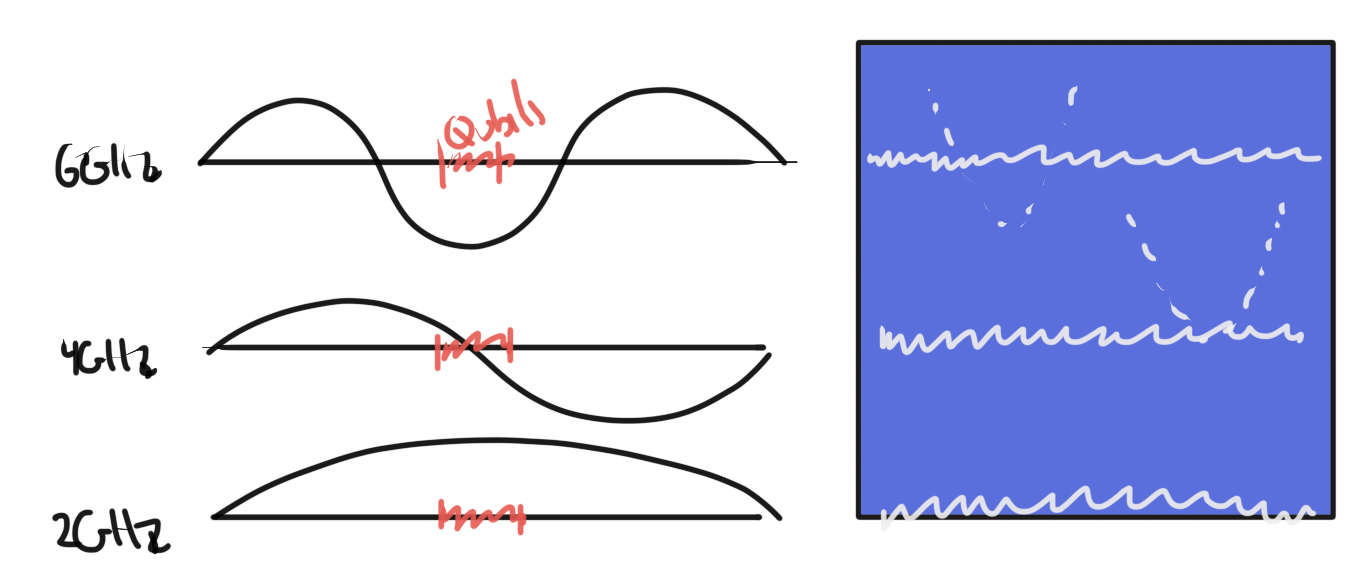
\includegraphics[height=5cm]{qubit_resonator1.png}
    \end{center}
    \noindent Tune  the VNA  (probe) to the  best resonance
    for your position of the qubit in \red{\textbf{two-tone
        measurements.}}
  \end{enumerate}
\end{framed}

\begin{framed}\noindent
  When making a resonator:
  \begin{enumerate}
  \item The length of  the resonator effects the wavelength
    $\lambda$ of the standing waves;
    
  \item Speed is determined by
    \begin{equation}
      \label{eq:resonator2}
      v = \frac{1}{\sqrt{LC}}.
    \end{equation}

    \noindent and in turn

    \begin{equation}
      \label{eq:resonator3}
      L      \propto  R \propto  \text{length}/\text{width};
    \end{equation}
    
  \item  Thus, in  order to  raise the  resonator frequency
    \red{\textbf{while keeping  the same standing  wave for
        interaction  with the  qubit}}, make  the resonator
    \red{\textbf{wider}}.
  \end{enumerate}
\end{framed}

\noindent A useful way of  figuring out which resonance you
are  firing   with  the   first  tone,   is  to   look  for
\textbf{vertical  lines}  in  the spectrum.   Whenever  the
qubit  cross \textbf{your  resonance}  (e.g.  resonator  at
3GHz, and  we move  to field  where the  qubit is  at 6GHz)
\red{\textbf{then irrelevant of  what the generator sweeps,
    the qubit will always be giving a response so you get a
    vertical white line.}}

\subsection{Choosing power}
\label{sec:choosing-power}

\begin{enumerate}
\item  For two-tone  measurements,  make  the probe  signal
  \red{1st  tone} fairly  weak so  that there  is a  single
  photon in the resonator.

  Keep  raising the  power,  until  resonator lines  become
  distorted.

\item The  generator signal  \red{2nd tone} should  be weak
  enough  to  get  a  thin  response  from  resonator,  but
  powerful enough to get a response at all.
\end{enumerate}

\newpage%
\section{Creating a dark state in a 3-level system\label{sec:dark_state}\cite{sillanpaa2009}\cite{abdumalikov2010}}
\iframe{We drive a 3-level system in such as way that one of it's states is never populated.}

We can use a flux qubit, solved in Chapter~\ref{sec:rfSquid}, for the 3-level system.
 
   \begin{figure}[h]
   	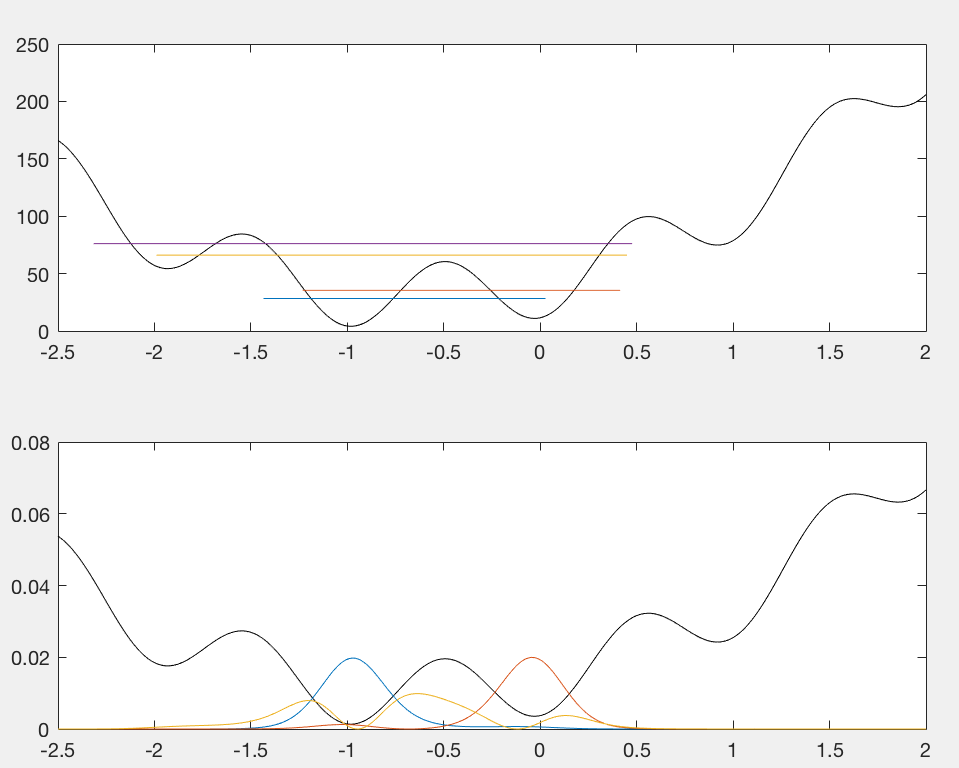
\includegraphics[height = 7cm]{rfSquid1} 	\includegraphics[height = 7cm]{rfSquid2}
   	\caption{\iket{0} migrates to the lower potential well as one increases the external flux. Black lines show the potential in the system.}
   	\label{fig:l3-myone}
   \end{figure}
  
 \subsection{Driving the three level atom\label{subsec:3LevelAtom}}  
  The Hamiltonian for a Three-Level atom, in a corresponding basis of eigenstates \iket{1}, \iket{2}, \iket{3}, by which the three levels are labelled, can be written as
  
  \begin{equation}
  \mathcal{H}_{\text{atom}} = \begin{pmatrix}
  E_1 & 0 & 0\\0& E_2 & 0 \\0&0&E_3
  \end{pmatrix}=\begin{pmatrix}
  E_3-\hbar\omega_{31} & 0 & 0\\0& E_3-\hbar\omega_{32} & 0 \\0&0&E_3
  \end{pmatrix},
  \label{rwaAtomicHamil}
  \end{equation}
  
  \noindent where $ \hbar\omega_{31} = E_3-E_1 $ and $ \hbar\omega_{32} = E_3-E_2$. Considering driving fields $ \Omega_{32} $, $ \Omega_{31} $ driving transitions \iket{2}\lra\iket{3} and \iket{1}\lra\iket{3} that arise due to capacitive or inductive coupling ($ \hbar\Omega_{ij} \propto \vartheta_{ij} $ is dervied in Chapter~\ref{sec:dipole_coupling})
  
  \begin{equation}
  \mathcal{H}_{\text{int}} = -\hbar\Omega_{31}\cos(\omega_{31}^{d}t) \begin{pmatrix}
  0 & 0 & 1\\0&0&0\\1&0&0
  \end{pmatrix}-\hbar\Omega_{32}\cos(\omega_{32}^{d}t) \begin{pmatrix}
  0 & 0 & 0\\0&0&1\\0&1&0
  \end{pmatrix},
  \label{rwaDriveHamiltonian}
  \end{equation}
  
  \noindent where the non-zero matrix elements indicate the states coupled by the fields. The total Hamiltonian, $ \mathcal{H}_{a} = \mathcal{H}_{\text{atom}}+\mathcal{H}_{\text{int}}$, is a sum of Eq.~\eqref{rwaAtomicHamil}, \eqref{rwaDriveHamiltonian}, written for convenience with complex exponentials,
  
  {\small \begin{equation}
  	\begin{aligned}
  	\mathcal{H}_{a}\ & {= \begin{pmatrix}
  		E_3-\hbar(\omega_{31}^{d}-\delta\omega_{31}) & 0 & -\frac{\hbar\Omega_{31}}{2}\bigg(e^{i\omega^{\text{d}}_{31}t}+e^{-i\omega^{\text{d}}_{31}t}\bigg)  \\   	0 & E_3-\hbar(\omega_{32}^{d}-\delta\omega_{32})  & -\frac{\hbar\Omega_{32}}{2}\bigg(e^{i\omega^{\text{d}}_{32}t}+e^{-i\omega^{\text{d}}_{32}t}\bigg)  \\   	-\frac{\hbar\Omega_{31}}{2}\bigg(e^{i\omega^{\text{d}}_{31}t}+e^{-i\omega^{\text{d}}_{31}t}\bigg)  & -\frac{\hbar\Omega_{32}}{2}\bigg(e^{i\omega^{\text{d}}_{32}t}+e^{-i\omega^{\text{d}}_{32}t}\bigg) & E_3 \\
  		\end{pmatrix}}\\& \qquad\qquad\qquad\qquad\qquad\qquad = \begin{pmatrix}
  	H_{11} & H_{12} & H_{13} \\   	H_{21} & H_{22} & H_{23} \\   	H_{31} & H_{32} & H_{33} \\
  	\end{pmatrix},
  	\end{aligned}
  	\label{rwaTotalHamiltonian}
  	\end{equation}}
  
  \noindent where $  \delta\omega_{31} = \omega_{31} - \omega^{\text{d}}_{31}, \delta\omega_{32} = \omega_{32} - \omega^{\text{d}}_{32}$ represent the detunings of the driving fields from the resonant frequencies of the atom. The Hamiltonian Eq.~\eqref{rwaTotalHamiltonian} governs the time evolution of the system state 
  
  \begin{equation}
  \ket{\varPsi} = c_1\ket{1}+c_2\ket{2}+c_3\ket{3},
  \end{equation} 
  
  \noindent through the standard \schrodinger equation, which takes on the matrix form
  
  \begin{equation}
  \begin{pmatrix}
  H_{11} & H_{12} & H_{13} \\   	H_{21} & H_{22} & H_{23} \\   	H_{31} & H_{32} & H_{33} \\
  \end{pmatrix}\begin{pmatrix}
  c_1\\c_2\\c_3
  \end{pmatrix} = i\hbar\begin{pmatrix}
  \dot{c_1} \\ \dot{c_2}\\\dot{c_3}
  \end{pmatrix}.
  \label{rwaTotalHamilMatrix}
  \end{equation}
  
  \noindent By applying a time dependent \red{\textbf{unitary transformation}}
  
  \begin{equation}
  \label{eqn:InteractionTransformation}
  \widetilde{c_i} = e^{i\phi_{i}(t)}c_i,
  \end{equation}
  
  \noindent where $ i=1,2,3 $, one can rewrite Eq.~\eqref{rwaTotalHamilMatrix} as
  
  \begin{equation}
  \begin{pmatrix}
  H_{11}-\hbar\dot{\phi}_1 & H_{12}e^{i\phi_{12}} & H_{13}e^{i\phi_{13}} \\  H_{21}e^{i\phi{21}} & H_{22}-\hbar\dot{\phi}_2 & H_{23}e^{i\phi{23}} \\   	H_{31}e^{i\phi{31}} & H_{32}e^{i\phi{32}} & H_{33}-\hbar\dot{\phi}_3 \\
  \end{pmatrix}\begin{pmatrix}
  \widetilde{c_1}\\\widetilde{c_2}\\\widetilde{c_3}
  \end{pmatrix} = i\hbar\begin{pmatrix}
  \dot{\widetilde{c_1}} \\ \dot{\widetilde{c_2}}\\\dot{\widetilde{c_3}}
  \end{pmatrix},
  \label{rawMatrixAfterTransformation}
  \end{equation}
  
  \noindent where $ e^{i\phi_{kj}} = e^{i(\phi_k-\phi_j)} $. Setting 
  
  \begin{equation}
  \phi_1 = \bigg(\frac{E_3}{\hbar}- \omega_{31}^d\bigg)t;\ \phi_2=\bigg(\frac{E_3}{\hbar}- \omega_{32}^d\bigg)t;\ \phi_3 = \frac{E_3}{\hbar}t,
  \label{rwaTransfomration}
  \end{equation}
  
  \noindent which effectively rotates the state vector components at the natural atomic evolution and detuning frequencies, \footnote{The full unitary transformation applied:
  	
  	$\qquad\qquad\quad U(t) = \exp\big[\frac{it}{\hbar}\left[({E_1}- \hbar\delta\omega_{31})\ketbra{1}{1}+({E_2}- \hbar\delta\omega_{32}\ketbra{2}{2})+E_{3}\ketbra{3}{3}\right]\big] $} will give a simple expression for the Hamiltonian
  
  \begin{equation}
  \widetilde{\mathcal{H}}_{a} = \begin{pmatrix}
  \hbar\delta\omega_{31} & 0 & -\frac{\hbar\Omega_{31}}{2}\\  0 & \hbar\delta\omega_{32} & -\frac{\hbar\Omega_{32}}{2} \\   	-\frac{\hbar\Omega_{31}}{2} & -\frac{\hbar\Omega_{32}}{2} & 0 \\
  \end{pmatrix} + \red{\begin{pmatrix}
  0 & 0 & -\frac{\hbar\Omega_{31}}{2}e^{-i2\omega^{d}_{31}t}\\  0 & 0 & -\frac{\hbar\Omega_{32}}{2}e^{-i2\omega^{d}_{32}t}  \\   	-\frac{\hbar\Omega_{31}}{2}e^{-i2\omega^{d}_{31}t} & -\frac{\hbar\Omega_{32}}{2}e^{-i2\omega^{d}_{32}t} & 0 \\
  \end{pmatrix}}.
  \label{rawTransformedFinal}
  \end{equation}
  
  \noindent In the rotating-wave-approximation, one ignores the contribution from the \red{fast rotating $ 2\omega^{d}_{31} $, $ 2\omega^{d}_{32} $} in the second term, since their oscillations will be averaged out at the time-scales of significant processes - physically they correspond to energy non-conserving processes. One is left with the following driving cases
  
  \begin{equation}
  \begin{aligned}
	  \label{rwaHamitlonianApprox}
	  \iket{1}\lra\iket{3} \text{ and } \iket{2}\lra\iket{3} & \quad 
	  	\widetilde{\mathcal{H}}_{a} = -\frac{\hbar}{2}
	  	\begin{pmatrix}
	  		-2\delta\omega_{31} & 0 & \Omega_{31}\\  0 & -2\delta\omega_{32} & \Omega_{32} \\   	\Omega_{31} & \Omega_{32} & 0
	  	\end{pmatrix};\\
	  \iket{1}\lra\iket{3} \text{ and } \iket{1}\lra\iket{2} & \quad 
	  	\widetilde{\mathcal{H}}_{b} = -\frac{\hbar}{2}
	  	\begin{pmatrix}
	  		0 & \Omega_{21} & \Omega_{31}\\  \Omega_{21} & 2\delta\omega_{21} & 0 \\   	\Omega_{31} & 0 & 2\delta\omega_{31}
	  	\end{pmatrix};\\
	  	\iket{1}\lra\iket{2} \text{ and } \iket{2}\lra\iket{3} & \quad 
	  		\widetilde{\mathcal{H}}_{c} = -\frac{\hbar}{2}
	  		\begin{pmatrix}
	  		0 & \Omega_{21} & 0\\  \Omega_{21} & 2\delta\omega_{21} & \Omega_{32} \\   	
	  		0 & \Omega_{32} & 2\delta\omega_{21} + 2\delta\omega_{32}
	  	\end{pmatrix}.
  \end{aligned}
  \end{equation}
  
  \noindent For various $ \delta\omega_{ij} \approxeq 0$, certain energy levels in the rotated frame become degenerate, shown in Fig.~\ref{theoRotation}b for a two level system. The off-diagonal terms induce a splitting $ \hbar\Omega $ between the eigenstates of the system,\footnote{For a Two-Level \iket{0}, \iket{1}, system,
  	
  	$\qquad\quad \mathcal{H} = \hbar\big(\begin{smallmatrix}0 & -\Omega/2\\-\Omega/2&0\end{smallmatrix}\big) $ has eigenenergies $ \pm\hbar\Omega $ and eigenstates $ \big(\iket{0}\mp\iket{1}\big)/\sqrt{2} $.} lifting this degeneracy. In the original unrotated frame, these Rabi splittings persist, resulting in a richer energy level structure as in Fig.~\ref{theoRotation}.
  
  \begin{figure}
  	\ifigure{4cm}{rotwave}
  	\caption{\textbf{The Rabi splitting of the energies in a Two-Level system.} A driving field with angular frequency $ \omega_{ij}^{d} $ and Rabi amplitude $ \Omega_{ij} $ in resonance with the atomic transition~$ \omega_{ij} $, couples the states \iket{i} and \iket{j}. In the rotated frame, the eigenstates $ \big(\iket{i}~\pm~\iket{j}\big)/\sqrt{2} $ are separated by an energy $ \hbar\Omega_{ij} $. Retuning to the original frame will map the Rabi splitting onto the original levels.}
  	\label{theoRotation}
  \end{figure}
  
  \newpage
  \subsection{Driving to the dark state\label{subsec:DoubleDrive}} 
  If $ \delta\omega_{32} = \delta\omega_{21} = 0 $ then Eq.~\eqref{rwaHamitlonianApprox} will read 
  
  \begin{equation}
	  \widetilde{\mathcal{H}}_{c} = -\frac{\hbar}{2}
	  \begin{pmatrix}
	  0 & \Omega_{21} & 0\\  \Omega_{21} & 0 & \Omega_{32} \\   	
	  0 & \Omega_{32} & 0
	  \end{pmatrix},
  \end{equation}
  
  \noindent with eigenvalues found from $ \det(\widetilde{\mathcal{H}}-\lambda\mathbb{I}) \equiv 0 $ and eigenvectors from $ (\widetilde{\mathcal{H}}-\lambda\mathbb{I})\vec{v} = 0 $:
   
   %  \eject \pdfpagewidth = 13in \pdfpageheight=10in
  \begin{equation}
	  \begin{aligned}
		  \red{E_0} &\red{= 0} & E_1 &= -\frac{\hbar}{2}\sqrt{\Omega_{21}^2+\Omega_{32}^2} & E_2 &= \frac{\hbar}{2}\sqrt{\Omega_{21}^2+\Omega_{32}^2}\\
		  \red{\vec{v}_0} & \red{= \frac{1}{\sqrt{\Omega_{21}^2 + \Omega_{32}^2}}
		  	\begin{pmatrix}
		  		\Omega_{32}\\0\\-\Omega_{21}
		  	\end{pmatrix}} & 
		  \vec{v}_1  & =
		  	\begin{pmatrix}
		  		\Omega_{21}\\ -\sqrt{\Omega_{21}^2 + \Omega_{32}^2} \\ \Omega_{32}
		  	\end{pmatrix} &
		 \vec{v}_2  & =
			 \begin{pmatrix}
		 		\Omega_{21}\\ \sqrt{\Omega_{21}^2 + \Omega_{32}^2} \\ \Omega_{32}
		 	\end{pmatrix},\\
	  \end{aligned}
  \end{equation}
   %    \eject \pdfpagewidth = 10in \pdfpageheight=10in
   
   \iframe{\noindent The state indicated in \red{red} is known as the dark state i.e. completely unpopulated \iket{1}. It happens when both the probe (\iket{0}\lra\iket{1}) and control (\iket{1}\lra\iket{2}) are on resonance:
   
   \[
   	\iket{\Psi_0} = \cos(\Theta)\iket{0} - \sin(\Theta)\iket{2};\qquad \tan(\Theta) = \frac{\Omega_{21}}{\Omega_{32}}.
   \]

	To get the ground state we do $ \sin(\Theta) = 0 \ra \Omega_p << \Omega_c $:
	\[
		\iket{\Psi_0}\approx \iket{0}
	\]
	}%

%% Quantum Phase Slip
\newpage

\section{Quantum phase slip \cite{mooij2005} \label{sec:qps}}

\subsection{Literature}
\begin{framed}\noindent
  \begin{itemize}
  \item \textbf{Charge control of blockade  of Cooper pair tunnelling in
      highly disordered TiN nanowires in an inductive environment}
    \begin{enumerate}
    \item Fabricate several thin superconducting bridges with meanders;
    \item Measure the  DC voltage, $ V  $, acorss then as  a function of
      the applied gate voltage, $ V_c $, from underneath the chip;
    \item Some samples have big oscillations  in $ V $ with gate voltage
      - Single  Electron Transistor regime, where  nanowire is compoased
      of grains, which feel a Coulomb Blockade;
    \item Quantum Phase Slip possible  in other samples, where there are
      no grains in the wire.
    \end{enumerate}
  \end{itemize}
\end{framed}

Initially quantum  phase slips  were a result  of thermal  activation in
thin wires.

\subsection{Cooper box duality}
The system  is dual to  the cooper pair  box system, where  the charging
energy  creates  a parabollic  dependence,  and  the Josephson  coupling
energy   $   E_J    $   mixes   states   lifting    degeneracy   as   in
Sec~\ref{sec:cooper_pair_box}:

 \begin{equation}\label{key}
   \mathcal{H} = E_c(\hat{n} - n_g)^2 - \frac{E_J}{2}\left[\iketbra{n+1}{n} + \iketbra{n}{n+1}\right].
 \end{equation}

 \noindent In the qunatum phase slip, we do the same thing, but now with
 inductor-component energy, $ E_L  = \frac{\Phi_0^2}{2L} $, is parabolic
 and degeneracy is lifted by the coupling, $ E_s $, due to the tunneling
 of fluxes (we do not specify yet the exact derivation of this energy):

 \begin{equation}\label{eq:hamiltonian-cqps-standalone}
   \mathcal{H} = E_L(\hat{n} - f)^2 - \frac{E_s}{2}\left[\iketbra{n+1}{n} + \iketbra{n}{n+1}\right],
 \end{equation}

 \noindent with $ f = \Phi/\Phi_0 $.

 \begin{framed}\noindent
   \noindent  The discussion  them stems  off into  how the  Cooper pair
   tunneling is  dual to the phase  slip, how one gets  similar steps in
   voltage current  characterisitics. There  is a lot  of math,  which I
   don't want to get into.
 \end{framed}

 \subsection{Mooij 2006 paper \cite{mooij2005}}
 \label{sec:mooij-2006-paper}

 \begin{equation}
   \begin{aligned}
     E_{L} & \equiv E_C\\
     E_{J} & \equiv E_s \\
     n_{g} & \equiv f
   \end{aligned}
 \end{equation}

 \noindent


\begin{figure}[h]
  \centering
  \includegraphics[height=7cm]{quantum-phase-slip/mooij_2005_energy_graphs}
  \caption{\small  The energy  spectra are  dual for  the two  systems -
    from. In  a) $E_C  >> E_J$  so that charge  is the  relevant quantum
    number  and  in  b) $E_L  >>  E_s$  so  that  phase is  the  quantum
    number. \cite{mooij2005}. \label{fig:mooij_2005_energy_graphs}}
\end{figure}

\subsection{Derivation}
\label{sec:derivation}

There  is  a  theory  written   in  the  book  \textbf{Devoret:  Quantum
  Fluctuation  in  electrical  circuits} about  how  \textbf{any  linear
  circuit   can  be   presented  by   an  equivalent   circuit  with   a
  frequency-dependent resistor}.

\begin{itemize}
\item  Current  biased: Resistor  is  in  parallel \hfill  Phase  across
  junction
\item Voltage biased: Resistor is in series \hfill No of CP transfered.
\end{itemize}

\begin{figure}[h]
  \centering
  \includegraphics[height=7cm]{quantum-phase-slip/mooij_2005_biases}
  \caption{\small  \textbf{JJ on  left} vs  \textbf{CQPS on  right}. The
    capacitor is replaced with an inductor to make phase the new defined
    quantum variable. \label{fig:mooij_2005_biases}}
\end{figure}

The main  transformation applied  that links the  following hamiltonians
(we    simply    match    the    inductive   and    QPS    terms    from
\autoref{eq:hamiltonian-cqps-standalone})  and  we   add  the  necessary
2$\pi$ factors
\begin{equation}
  \begin{aligned}
    \mathcal{H}_{JJ} & = E_C\hat{q}^2 - E_J\cos\hat{\varphi} \\
    \mathcal{H}_{CQPS}   &  =   E_L\frac{\hat{\varphi}^2}{(2\pi)^{2}}  -
    E_S\cos(2\pi\hat{q})
  \end{aligned}
\end{equation}

\noindent This requires the following set of transformations:

\begin{itemize}
\item $\hat{q} \rightarrow - \frac{\varphi}{2\pi}$
\item $\hat{\varphi} \rightarrow 2\pi q$
\item $E_s \rightarrow E_J$
\item $E_L \rightarrow E_C$
\item $I \Leftrightarrow \frac{V}{R_{q}}$
\item $Y(\omega) \Leftrightarrow \frac{Z(\omega)}{R_q^2}$
\end{itemize}

\subsection{Inverse shapiro steps}
\label{sec:inverse-shap-steps}

Now  if we  take  the  aforementioned mappings  and  apply  them to  the
equation used to model a typical JJ

\begin{figure}[h]
  \centering \inkfig{8cm}{typical_jj_setup}
  \caption{\small Modelling a JJ\label{fig:typical_jj_setup}}
\end{figure}

\begin{equation}
  I(t) = \red{I_c\sin\varphi} + \frac{\Phi_{0}}{2\pi}\left[ \green{C \frac{d^2\varphi}{dt^{2}}} + \blue{\frac{1}{R}\frac{d\varphi}{dt}} \right]
\end{equation}

\noindent  which  leads  to  Shapiro steps.  \red{Add  explanation  from
  metrology notes}.

Upon subbing in
\begin{equation}
  V(t) = \red{V_c\sin(2\pi q)} + 2e\left[ \green{L \frac{d^2q}{dt^{2}}} + \blue{R\frac{dq}{dt}} \right]
\end{equation}

\noindent where we  now deal with the voltage drops  across the CQPS (in
becomes a linear circuit). \textbf{Valid when the charge is the relevant
  quantum number (just like for JJ phase is the quantum number as we are
  localised in a potential minimum)}

\red{TODO: Plasma frequency in JJ.}

\newpage

%%% Local Variables:
%%% mode: latex
%%% TeX-master: "all_the_notes"
%%% End:
%
\newpage
\section{Single Photon}
\label{sec:single-photon}

\begin{itemize}
\item High efficiency;
\item On-demand, deterministic operation;
\item Low timing jitter;
\item Control shape of wave packet \cite{Forn_D_az_2017}
\end{itemize}

\subsection{What is spectral density}
\label{sec:what-spectr-dens}

An excellent  paper \cite{Hoi_2015} says  that \textbf{for an atom  to transition
  \iket{1} \ira \iket{0} the rate of transition, according to \red{Fermi's golden
    rule}, is proportional to the spectral density of electromagnetic modes}.

\begin{framed}\noindent
  Thus,  measuring lifetime  of  an  atom probes  the  local  strength of  vacuum
  fluctuations  at that  transition  frequency.  \textbf{The  frequency-dependent
    spatial structure of the vacuum}
\end{framed}

Once a relaxation occurs, a photon of frequency $\omega_{\text{qubit}}$ and wavelength

\begin{equation}
  \lambda(\Phi) = \frac{2\pi v}{\omega_{\text{qubit}}}, \quad v = \frac{1}{\sqrt{lc}}
\end{equation}

\noindent is emitted into the line.

\subsection{Making measurement}
\label{sec:making-measurement}

For normalisation,  subtract the reference when  the photon source it  turned off
for the different measurements \cite{Pechal_2016}:
\begin{itemize}
\item Power (\iabs{V})
\item $\left|\iaverage{a}\right|$
\item $\iaverage{a^{\dagger}a}$
\item $\iaverage{a^{\dagger}a^{\dagger}aa}$
\end{itemize}

\begin{figure}[h]
  \centering
  \includegraphics[height=8cm]{2016_pechal_superconducting-switch-for-fast-on-chip-routing-of-quantum-microwave-fields/single-photon-moments}
  \caption{\small Ignore  the green line.   $a \propto $ equator  component (coherent),
    and      $a^{\dagger}a     \propto      $     relaxation      from     excited      state
    (incoherent) \label{fig:single-photon-moments}}
\end{figure}

\noindent

%%% Local Variables:
%%% mode: latex
%%% TeX-master: "all_the_notes"
%%% End:
%

%%% Hard theory
\newpage
\section{Simulating circuits \label{sec:simulating_circuits}}
 Oleg went through how one would simulate a circuit, such as the one below (in fact this is the setup for the inverse Shapiro step):
 
  \ipic{5cm}{circuit_inverse_shapiro}
 
 \noindent Constraints in this system are that we solve the current for
 \begin{itemize}
 	\item Work with $ n $ \hfill number of CP of charge $ \mathbf{2e} $;
 	\item $ V $ \hfill the DC voltage that we fix;
 	\item $f$ \hfill is the frequency of the rf-bias.
 	\item \red{Ignore that large capacitance $ C $} - it's so large that it has no effect on the whole system.
 \end{itemize}
 
 \noindent Next we write out a system of simultaneous equations that Oleg solves numerically in \verb|Mathematica| for $ n(t) $.
 
 \begin{equation}\label{key}
 	\left\lbrace\begin{aligned}
 		V & = \red{2eR\dot{n}} + \blue{\frac{2e}{C_a}n_2}\\
 		V & = \red{L\frac{d}{dt}(\dot{n}-\dot{n}_2)} + \blue{\frac{2e}{C_b}(n_3 - n_4)}  \green{- V_{rf}\cos(2\pi ft)}\\
		V & = \red{L\frac{d}{dt}(\dot{n}-\dot{n}_2)} + \blue{\frac{2e}{C_c}n_3}
 	\end{aligned}\right.
 \end{equation}
 \begin{itemize}
 		\item \red{Charge passing through resistor $ R $ and inductor, $ V = L\dot{I} $};
 		\item \blue{Potential difference across capacitors due to onset charge};
 		\item \green{RF-voltage source in action}.
 \end{itemize}
 
 \noindent What we find if oscillations in this charge number $ n_1(t) $. Evaluating $ \iaverage{I(V)} = \int_{t_1}^{t_2}2e n(t)dt $ for different bias voltages $ V $, we can plot a $ V \text{ vs } \iaverage{I(V)} $ graph, which will show Shapiro steps.
 
 \ipic{4cm}{inverseShapiro_oscillations}.%
\section{Properties of photons}
 If we have a decay of radiation
 \begin{equation}\label{key}
 	E^{(+)}(t) = E_0e^{-2\pi i \nu_0t}e^{-\frac{\kappa}{2}t}
 \end{equation}
 
 \noindent and take its Fourier transform, we get a Lorentzian, with an intensity
 
 \begin{equation}\label{key}
 	\iabsSquared{f(\nu)} = \frac{4\iabs{E_0}^2}{\kappa^2 + \iabsSquared{4\pi(\nu_0 - \nu)}}.
 \end{equation}
 
 \iframe{
 	It has a half-width of
 	\begin{equation}\label{key}
 		\Delta\nu = \frac{\kappa}{2\pi},
 	\end{equation}
 	\noindent and since $ \Delta t = \kappa^{-1} $, we get the relationship
 	
 	\begin{equation}\label{key}
 		\Delta\nu\Delta t \approx \frac{1}{2\pi}
 	\end{equation}
	}

 \subsection{Emission and line broadening}
  Classically, we have en ensembled of atom, the relaxing \iket{2}\ra\iket{1}. If we hit particles to take away the `unradiated' energy, the relaxation terminates, and atoms emit only part of the full energy $ \hbar\omega_{21} $. Because this is an ensembled, on average the energy $ \hbar\omega_{21} $ will still be emitted, just with a smaller $ \Delta t $, so the line broadens.
  
  Quantum mechanically, we cannot emit `parts' of $ \hbar\omega_{21} $. Either the photon is emitted, or the photon is not. \red{Absurdly, if tha atom has been emitting for a certain time, and then the energy is taken away (say during a collision), then it is free to \textbf{track back} and not release the photon, or release it fully.}
 
 \subsection{Classical vs Quantum pulses}
  Suppose that an atom emits a photon of frequency $ hf $ and we start catching it by a localised detector (or just leave it to interact with the environment, which implicitly performs measurements for us)
  \begin{itemize}
  	\item \underline{Classically} the energy is spread out over space \ra \textbf{we never measure the total energy of the pulse};
  	\item \underline{Quantum} the photon will be absorbed or not absorbed at different points in space. Performing an average over all the positions, we find an exponential decay with a vertical front.
  \end{itemize}
 
 Now, when emission takes place, the wavefunction evolves from $ \Psi_2\Phi_{\text{vacuum}} $ to
 
 \begin{equation}\label{key}
 	e^{-\frac{\Gamma}{2}t}\Psi_2\Phi_{\text{vacuum}} + \sqrt{1-e^{-\Gamma t}}\Psi_1\Phi_{\text{photon}(t)}.
 	 \end{equation}
 
 What is important here?
 \begin{itemize}
 	\item Upon measurement, the wavefunction collapses to one of the two states: 1) either the atom is still excited; 2) the photon has been emitted;
 	\item As the relaxation occurs, $ \Phi_{\text{photon}}(t) $ evolves, to have a smaller and smaller `tail' in the atom. The change occurs over a time $ \Gamma^{-1} $.
 	 \iframe{When the atom gives all its excitation energy away during a collision and nothing is left to the radiation field, the atom need not “reel back” any field because, until that moment, no real emission took place. The latter emission happened only virtually – whatever that
 		might mean!}
 	\item If we leave the system for long enough, it will, by itself, transfer irreversibly to state $ \Psi_1\Phi_\text{photon} $ (normally quantum mechanics is reversible, as long as measurement is not made);
 	\item The photon has a size
 	\begin{equation}\label{key}
 		cT = \frac{c}{\Gamma}.
 	\end{equation}
 	\noindent This extension explains interference effects
 	\iframe{
 		The photon is spread over space \textbf{before} measurement, with a distribution:
 		\begin{equation}\label{key}
 			\iaverage{\hat{E}^{(-)}(\mathbf{r},t)\hat{E}^{(+)}(\mathbf{r},t)},
 		\end{equation}
 		\noindent \red{and the probability of detectors response is propotional to it}.
 		
 		\red{\textbf{Upon each measurement the photon will be localised in a single space, as the wavefunction collapses.}} Two important errors are:
 		\begin{itemize}
 			\item The photon is not localised before measurement - it's not a particle, it's a wavefunciton with collapses only upon detection;
 			\item The photons energy is not spread out - it's not a wave, it's a wavefunction.
 		\end{itemize}
 	}
 	\item Photons are never split \ra in this case we would have photons of energy $ \frac{1}{2}hf $, which would dissapear from the observable world, as they have no atoms to be absorbed with.
 	\item For interference we need two beams from the same source, so that phase fluctuations are the same - same as in the master beam.

 	\iframe{But what if now, we measure over a timescale \red{of the order of the coherence time}, preventing washing out of the pattern? This was done with lasers (enough power to have many photons for clear interference) and an interference pattern was setup.}
 	
 	\item A really cool way to measure interference patterns with very weak sources, is to take two beams, and beam split each one. 
 	\begin{itemize}
 		\item The stronger beams should intefere on a controlled detector. The interference pattern will constantly change (as the phase changes randomly in each beam). We pick on such pattern, and produced a square pulse \textbf{only} when it is formed;
 		\item This pulse is used to open a shutter on another screen, where the weaker beams are sent through. Thus, we will be building up a pattern of the two beams at a fixed phase, even though they come from two sources!
 	\end{itemize}
 	Note that for such weak intensities, the photon picture of light completely fails - if they were partciles then its extremely improbable that both will be passing throught the shutter at the same time to interfere with one another. Here light behaves more like a wave.
 \end{itemize}

 \subsection{More about photons}
  We can also apply laser pulses to form superpositions of 2 atomic states. It is possible for the system to transition into one energy level simultaneously. \red{The emitted photon will have elements of both excited atomic states - this will show up as the photon having two frequencies!}
  
  \ipicCaption{6cm}{photon_beating}{Suppose that we create a superposition in the atom $ \frac{\iket{1}+\iket{2}}{\sqrt{2}} $. Then there are two possible ways for the atom to decay to the ground energy state and create an outgoing photon. When we measure the intensity of the photon, with the outgoing detector, the photons 1\ra0 and 2\ra0 components will interfere to produed beatings. The photon is thus imprinting the full information of the atomic excitation. \red{Oh, did I mention this is a single photon? Classically this would be impossible to do with a single photon.}}

 \begin{itemize}
 	\item \textbf{Parametric fluorescence:} during parametric down conversion in a non-linear medium, a single photon spontanesouly decays into two more (idler and signal), abiding energy and momentum conservation:
 	
 	\begin{equation}\label{key}
 		\begin{aligned}
	 		\hbar(\omega_p) & = \hbar(\omega_i + \omega_s);\\
	 		\hbar\mathbf{k_p} & = \hbar(\mathbf{k_i} + \mathbf{k_s}).
 		\end{aligned}
 	\end{equation}
 	
 	\noindent The emitted photons become entangled and will have a very strong correlation in terms of total energy and simultaneous mesasurement.
 	
 	Such fluorescence photons are good to use as single photon sources - registering the idler photon, we can be 100\% sure that a corresponding signal photon is flying in a specific direction
 	\item Now consider forming an interference pattern with photons. The clarity of the interference pattern depends on the uncertainty of the phase, $ \Delta\phi $. The phase and photon number abide the relationship
 	\begin{equation}\label{key}
 		\Delta n\Delta\phi \ge\frac{1}{2},
 	\end{equation}
 	\noindent so surely with decreasing photon number (decreasing $ \Delta n $), the phase should diverge and wash out interference! \iRa In reality the phase uncertainty accumulates in the vacuum state \iket{0}, which does not contribute to the interferene pattern.
 	\item To ensure good matching of frequencies from two sources, one can measure beats in interference patterns, and only open the shutter when the beats oscillate slowly (good frequency matching).
 \end{itemize}

 \subsection{Photon bunching}
  We begun with discussing that when observing stars. We use something similar to an interferometer, and pick up an interference pattern on the telescope screen.
  
  Now consider a second light source (different part of the planet). It will fly in at an ever small different angle, and \textbf{its' pattern will be shifted, relative to the initial one}. An overlap will occur if we increse the separation of the telescope mirrors (increasing the phase difference between the patterns). \red{This is called the coherence length - separation at which interference vanishes}
  
  \iframe{Probability that two photons arrive at the same place shrotly one after another i.e. $ \tau < t_{\text{coh}} $ is higher than if they arrive with a larger time delay $ \tau > t_\text{coh}. $

	\textbf{\Huge This is exactly analogous to the coherene length above, except in time!}
}
  
  If one thinks in the photon pitcture, this implies that photon sources communicate with each other to release photons in pairs. \red{\textbf{But this is seriously wrong!} It is actually do do with inteference between the waves emitted by completely different atoms!}

 \subsection{Types of light}
 \iframe{\red{\textbf{Coherence volume}} \red{or time} is over which the \textbf{instantaenous} phase does not change significantly within it.
 \newline
 
 The photon number is related to the mode volume $ V_\text{coherence} $. In experiments we must be working within this volume, or within the related time $ T $, over which coherence persists. \red{If a fraction of the volume (time) is observed, then only a fraction of photons present are observed}
}
  \begin{enumerate}
  	\item   \textbf{Thermal light, is formed of partial waves with random phases.} The intensity fluctuates in time. \red{The bandwidth of scattered light is very narrow}, giving a large $ \Delta t $ for intensity correlation measurements.
  	
  	It follows a Bose einstein distribution which is very broad and \textbf{the photons are subject to bunching!}
  	
  	\item \textbf{Laser light} has a constant amplitude (intensity) and follows a Poisson distribution, which is much narrower than the Bose one for thermal light.
  	
  	\ipic{6cm}{photon_distribution}
  	
  	Laser light does not tend to bunch (unlike thermal light) with the coincidence photon rate being the same as the random one - same probability of detecting photons for all kinds of different time delays.
  \end{enumerate}

 \subsection{Photon antibunching}
  \iframe{Occurs with photons with a sharp photon number \iaverage{n}.}
  So now consider the case of a detector, which accumulates over a time (or volume) $ V_\text{obs} $. It has probability
  
  \begin{equation}\label{eqn:bookQO_1}
  	t = \frac{V_\text{obs}}{V_\text{coh}}\eta,
  \end{equation}
  
  \noindent of detecting a photon, which depends on the ratio of the observed to the coherence volume (\textbf{recall that photon numbers are associated with the mode volume $ V_\text{coh} $, so if we observe a smaller volume, than we register a fraction of the photons.})
  
  The detector either detects or photon (with probabiltiy $ t $) or it doesn't. So the probability of transmitting $ k $ out of $ n $ photons follows a binomial distribution
  
  \begin{equation}\label{key}
  	\text{Prob(k photons)} = \imatrixcol{n}{k}t^{k}r^{n-k},
  \end{equation}
  
  \noindent which has a variance
  
  \begin{equation}\label{key}
  	\Delta k^2 = (1-t)\iaverage{k} \qquad (\equiv \iaverage{k^2} - \iaverage{k}^2).
  \end{equation}
  
  \noindent Now, look out!
  \begin{itemize}
  	\item The lower the detection probabulity in Eq.~\eqref{eqn:bookQO_1}, due to shorter integration time or lower efficiency, the large the variance $ \Delta k^2 $.
  	\item If however we are able to detect all photon in the mode volume $ V_\text{coh} $, then there should be no variance.
  \end{itemize}

 \iframe{\red{Unlike with bunched light, where photon number is undefined, the ratio of random clicks to simulatneous clicks}
 
 \begin{equation}\label{key}
 	R = \frac{\Delta n^2 - \iaverage{n}}{\iaverage{n}^2},
 \end{equation}
 \noindent \red{can be negative! \textbf{Negative relative to the counts we would measure outside the coherence time/volume, where statistics were random.}}
 
 This is showing photon antibunching, whereby photon do not tend to be simultaneously detected in the same coherence volume.
}
 
 Let us disuss this more fully
 \begin{itemize}
 	\item Classically the coincidence coutning rate (simultaneous clicks) $ \propto I(t)I(t+\tau) $, which has a maximum at $ \tau = 0 $ (opposite of antibunching);
 	\item \textbf{Antibunching:} (Sub-)Poisson statistics for \iaverage{n} \ra 0. $ \Delta n < \iaverage{n}$. \red{Only when we fire single photons.};
 	\item \textbf{Bunching:} Poisson statistics for \iaverage{n} \ra $ \infty $. $ \Delta n > \iaverage{n} $.
 	\item 
 \end{itemize}

 \subsection{Creating antibunching}
  To create a stream of bullets (which is not how we imagined light classically - we used to think of it as a wave)
  \begin{itemize}
  	\item Use atoms flying through cavity \ra excite and allow some of them to relax \ra then measure with an ionisation detector to recover photon statistics from the de-excited atom statistics;
  	\item Create electron hole pairs and create light emission in a controlled way;
  \end{itemize}
 
 \subsection{Squeezed light}
  Squeezed light has a $ \Delta x $ or $ \Delta p $ smaller than vacuum. The other component is correspondingly blown up. These two quantities arise when we rewrite the field
  
  \begin{equation}\label{key}
  	\mathbf{E}(\vec{r},t) = Ae^{i(\vec{k}\vec{r} - \omega t)} + A^{*}e^{-i(\vec{k}\vec{r} - \omega t)},
  \end{equation}
  
  The quantum mechanical description of the field is
  \[
  	\hat{E} = \hat{E}^{(+)} + \hat{E}^{(-)} = e^{-i\omega t}\hat{a} + e^{i\omega t}\hat{a}\idagger,
  \]
  
  \noindent \red{where the amplitude is replaced with the quantum mechanical field operators, telling how many photons are in the field.} The energy of the field is
  
  \[
  	\hat{H} = \hbar\omega\hat{a}\idagger\hat{a}
  \]
  
  \iframe{\begin{itemize}
  		\item Electric field strength \iaverage{\hat{E}} = 0 for states with well defined photon number \iket{n}. (The $ \hat{a} $ operators raise and lower this number, so that the product of two different `kets' is 0.)
  \end{itemize}}
  
  \noindent in terms of two new variables $ x = \re{A}, p =\im{A} $
  
  \begin{equation}\label{key}
  	E(\vec{r},t) = C\bigg[x\cos(\omega t - \vec{k}\vec{r}) + p\sin(\omega t - \vec{k}\vec{r})\bigg]
  \end{equation}
  
 \subsection{Phase distribution}
  Say we want to measure the phase distribution of the field
  
  \begin{equation}\label{key}
  	E(z,t) \propto \cos(\omega t - \phi - kz),
  \end{equation}
  
  \noindent which we rewrite
  
  \begin{equation}\label{key}
  	\begin{aligned}
  		\cos(\phi)& \cos(\omega t - kz) &+ \sin(\phi)&\sin(\omega t - kz)\\
  		\frac{x}{\sqrt{x^2+p^2}} & \cos(\omega t - kz) &+ \frac{p}{\sqrt{x^2+p^2}}&\sin(\omega t - kz)\\
  	\end{aligned}.
  \end{equation}
  
  \iframe{So by measuring the quadrates of the field, we can map out the x and the p components. The are multiple ways of describing $ x,p $ distribution in phase space (where distance from axis, $ \rho $, is amplitude, and angle, $ \phi $:
  	\begin{itemize}
  		\item Through the Q function
  		\begin{equation}\label{key}
  			w(x,p) = \frac{1}{\pi}\iabsSquared{\bra{\psi}\ket{\alpha}},
  		\end{equation}
  		\noindent which looses some information about the $ x $ and $ p $ distribution, due to them being non commutable observables;
  		\item Wigner function, which gives full information about the state
  		\begin{equation}\label{key}
  			W(x,p) = \frac{1}{\pi}\int_{-\infty}^{\infty}e^{i2py}\psi(x-y)\psi^{*}(x+y)dy.
  		\end{equation}
  		\noindent This turns into the Q function, if we convolute it with a Gaussian, which smooths the function out.
  	\end{itemize}
  	)}
  
\newpage %

%%% Base theory i.e. I have a good understanding of this
\section{Interaction picture \label{sec:interaction}}
Given an eigenstates of $\hat{H}_0$, we can easily compute the system evolution 

\begin{equation}
\ket{\psi(t)} = \sum_j\alpha_je^{-iE_jt/\hbar}\ket{\phi_j}.
\end{equation} 

Now to find the state for a system with a Hamiltonian 

\begin{equation}
\hat{H} = {H}_0 +V,
\end{equation}

\noindent we define the interaction picture state

\begin{equation}
\ket{\psi(t)}_I = U_0(t)^\dagger\ket{\psi(t)}_S,
\end{equation}

\noindent Substituting $\ket{\psi(t)}_S = U_0(t)\ket{\psi(t)}_I$ into the Schrödinger equation $i\hbar\frac{\partial}{\partial t}\ket{\psi(t)}_S = \hat{H}\ket{\psi(t)}_S$

\begin{equation}
\begin{aligned}
i\hbar\frac{\partial}{\partial t}\left(U_0(t)\ket{\psi(t)}_I\right) = i\hbar\left(U_0(t)\frac{\partial\ket{\psi(t)}_I}{\partial t} + \frac{-iH_0}{\hbar}U_0(t)\ket{\psi(t)}_I\right) \equiv HU_0(t)\ket{\psi(t)}_I,
\end{aligned}
\end{equation}

\noindent multiplying by $U_0^\dagger(t)$

\begin{equation}\label{eqn:interactionPictureHamiltonian}
\begin{aligned}
i\hbar\ipartial{\ket{\psi(t)}_I}{t} & = H_I\ket{\psi(t)}_I\\
& H_i = U_0^\dagger(t)\left[H-H_0\right]U_0(t) = U_0^\dagger(t)\left[V\right]U_0(t).
\end{aligned}
\end{equation}

\red{\textbf{\large Ultimately, what we have found is that to solve for $H=H_0+V$, one needs to}}
\textcolor{red}{\begin{enumerate}
		\item Find $H_I = U_0^\dagger(t)VU_0(t)$
		\item Solve the interaction Scrodinger equation $i\hbar\ipartial{\ket{\psi(t)}_I}{t} = H_I\ket{\psi(t)}_I$
		\item Find the Schroinger picture states by unwinding i.e. $\ket{\psi(t)}_S = U_0(t)\ket{\psi(t)}_I$
\end{enumerate}} 

It can be easily shown that expectation values are preserved

\begin{equation}
_I\bra{\psi}\hat{O}_I\ket{\psi}_I = _S\bra{\psi}U_0U_0^\dagger\hat{O}_SU_0U_0^\dagger\ket{\psi}_s \equiv _S\bra{\psi}\hat{O}_S\ket{\psi}_S
\end{equation}

\newpage 
\section{Interaction between light and atom \label{sec:lightAtom}}
We construct the Hamiltonian for the full system

\begin{equation}
\hat{H} = \hat{H}_\text{atom} + \hat{H}_\text{light} + \hat{H}_\text{atom - light}. 
\end{equation}

\begin{itemize}
	\item $\hat{H}_\text{atom}$ comes from the energy levels of the atom
	\begin{equation}
	\label{eqn:atomHamiltonian}
	\hat{H}_\text{atom} = \hbar\omega_a\ketbra{e}{e}\otimes\mathbb{I}_\text{light},
	\end{equation}
	
	\item $\hat{H}_\text{light}$ from Sec.\ref{subsec:singleMode} is the Hamiltonian for the photon modes
	\begin{equation}
	\label{eqn:lightHamiltonian}
	\hat{H}_\text{light} = \mathbb{I}_\text{atom} \otimes \hbar\omega_j\left(\hat{a}^\dagger\hat{a}+\frac{1}{2}\right),
	\end{equation}
	
	\item and $\hat{H}_\text{atom - light} = - \hat{E}\cdot \hat{D} $ from Sec.\ref{sec:dipole}
	\begin{equation}
	\begin{aligned}
	\hat{H}_\text{atom - light} & = - \left(\mathbf{E_{0x}}(\hat{a}+\hat{a}^\dagger)\mathbf{\red{\sin(kz)}}\right)\left(\red{\mathbf{\vec{d}}}\left(\ketbra{g}{e}+\ketbra{e}{g}\right)\right)\\
	& = \mathbf{\red{\hbar g(\vec{r})}}\left(\hat{a}+\hat{a}^\dagger\right)\left(\ketbra{g}{e}+\ketbra{e}{g}\right),
	\end{aligned}
	\end{equation}	
\end{itemize}  

\noindent where \red{$\hbar g(\vec{r}) = E_{0x}\sin(kz)\vec{d}$} is the coupling strength. Although ideally we should be writing state via the tensor product notation, we shall do this instead save space and write

\begin{equation}
\ket{g,n}=\ket{g}\otimes\ket{n}
\end{equation}

\noindent The full Hamiltonian is then

\begin{equation}
\hat{H} = \hbar\omega_a\ketbra{e}{e} + \hbar\omega_j\left(\hat{a}^\dagger\hat{a}+\frac{1}{2}\right) + {\hbar g(\vec{r})}\left(\hat{a}+\hat{a}^\dagger\right)\left(\ketbra{g}{e}+\ketbra{e}{g}\right),
\end{equation}

\noindent which we split up into two parts, to use the interaction picture, covered in Sec.\ref{sec:interaction}

\begin{equation}
\left\lbrace 
\begin{aligned}
H & = H_0+\red{V}\\
H_0 & = \hbar\omega_a\ketbra{e}{e} + \hbar\omega_j\left(\hat{a}^\dagger\hat{a}+\frac{1}{2}\right)\\
\textcolor{red}{V} & \red{=} \textcolor{red}{{\hbar g(\vec{r})}\left(\hat{a}+\hat{a}^\dagger\right)\left(\ketbra{g}{e}+\ketbra{e}{g}\right)}
\end{aligned}\right.
\label{eqn:lightAtomHamiltonians}
\end{equation}

\noindent We compute the interaction Hamiltonian

\begin{equation}
\left\lbrace
\begin{aligned}
H_I & = U_0^\dagger V U_0 \\
U_0 & = \exp\left[-i\omega_j\left(\hat{a}^\dagger\hat{a}+{1}/{2}\right)t\right]\exp\left[-i\omega_a\ketbra{e}{e}t\right]
\end{aligned}\right. \Rightarrow
\end{equation}

\begin{multline}
\Rightarrow \textcolor{red}{\hbar g(\vec{r})} \times \\
\exp\left[+i\omega_j\left(\hat{a}^\dagger\hat{a}+{1}/{2}\right)t\right]\textcolor{red}{\left(\hat{a}+\hat{a}^\dagger\right)}\exp\left[-i\omega_j\left(\hat{a}^\dagger\hat{a}+{1}/{2}\right)t\right] \times\\
\exp\left[+i\omega_a\ketbra{e}{e}t\right]\textcolor{red}{\left(\ketbra{g}{e}+\ketbra{e}{g}\right)}\exp\left[-i\omega_a\ketbra{e}{e}t\right]
\end{multline}

\noindent Then we proceed term by term
\begin{itemize}
	\item $\exp\left[+i\omega_j\left(\hat{a}^\dagger\hat{a}+{1}/{2}\right)t\right]\textcolor{red}{\hat{a}}\exp\left[-i\omega_j\left(\hat{a}^\dagger\hat{a}+{1}/{2}\right)t\right] = \exp\left[+i\omega_j\hat{a}^\dagger\hat{a}t\right]\textcolor{red}{\hat{a}}\exp\left[-i\omega_j\hat{a}^\dagger\hat{a}t\right]$
	
	The lowering operator \textcolor{red}{
		\begin{equation}
		\begin{aligned}
		\hat{a} & =
		\begin{bmatrix}
		\bra{0}\hat{a}\ket{0} & \bra{0}\hat{a}\ket{1} & \cdots\\
		\bra{1}\hat{a}\ket{0} & \bra{1}\hat{a}\ket{1} & \cdots\\
		\bra{2}\hat{a}\ket{0} & \bra{2}\hat{a}\ket{1} & \cdots\\
		\vdots & \vdots & \ddots\\
		\end{bmatrix}
		= \begin{bmatrix}
		\bra{0}0 & \bra{0}\sqrt{1}\ket{0} & \cdots\\
		\bra{1}0 & \bra{1}\sqrt{1}\ket{0} & \cdots\\
		\bra{2}0 & \bra{2}\sqrt{1}\ket{0} & \cdots\\
		\vdots & \vdots & \ddots\\	
		\end{bmatrix}
		= \begin{bmatrix}
		0 & \sqrt{1} & \cdots\\
		0 & 0 & \cdots\\
		0 & 0 & \cdots\\
		\vdots & \vdots & \ddots\\	
		\end{bmatrix}\\
		& = \sum_n\sqrt{n}\ketbra{n-1}{n}
		\end{aligned}
		\end{equation}}
	
	\noindent and thus evaluating
	
	\begin{equation}
	\begin{aligned}
	e^{+i\omega_jt\hat{a}^\dagger\hat a} & \left[\sum_n\sqrt{n}\ketbra{n-1}{n}\right]e^{+i\omega_jt\hat{a}^\dagger\hat a}\\
	& = \sum_n \sqrt{n}e^{+i\omega_jt\hat{a}^\dagger\hat a}\ket{n-1}\bra{n}e^{-i\omega_jt\hat{a}^\dagger\hat a} \qquad \leftarrow\text{ expand exponential operator}\\
	& = \sum_n \sqrt{n}e^{+i\omega_j(n-1)t}\ket{n-1}\bra{n}e^{-i\omega_jnt}\\
	& = e^{+i\omega_j(n-1)t}\left[\sum_n \sqrt{n}\ket{n-1}\bra{n}\right]e^{-i\omega_jnt}\\
	& = e^{+i\omega_j(n-1)t}\hat{a}e^{-i\omega_jnt}\\ & \blue{\mathbf{\equiv  \text{\textbf{exp}}[-i\omega_jt]\hat{a}}}
	\end{aligned}
	\end{equation}
	
	\item $\exp\left[+i\omega_j\left(\hat{a}^\dagger\hat{a}+{1}/{2}\right)t\right]\textcolor{red}{\hat{a}^\dagger}\exp\left[-i\omega_j\left(\hat{a}^\dagger\hat{a}+{1}/{2}\right)t\right] = \blue{\mathbf{\text{\textbf{exp}}[+i\omega_jt]\hat{a}^\dagger}}$
	
	\item \begin{equation}
	\begin{aligned}
	\exp\left[+i\omega_a\ketbra{e}{e}t\right]&\textcolor{red}{\ketbra{g}{e}}\exp\left[-i\omega_a\ketbra{e}{e}t\right] \\
	& = \bigg[\exp\left[+i\omega_at\left(\mathbb{I} - \ketbra{g}{g}\right)\right]\textcolor{red}{\ket{g}}\bigg]\bigg[\textcolor{red}{\bra{e}}\exp\left[-i\omega_a\ketbra{e}{e}t\right]\bigg]\\
	& = \bigg[\exp\left[+i\omega_at\left(1 - 1\right)\right]\textcolor{red}{\ket{g}}\bigg]\bigg[\textcolor{red}{\bra{e}}\exp\left[-i\omega_a1t\right]\bigg]\\
	& = \bigg[\exp\left[+i\omega_at0\right]\bigg]\textcolor{red}{\ket{g}}\textcolor{red}{\bra{e}}\bigg[\exp\left[-i\omega_at\right]\bigg]\\
	& \blue{\mathbf{\equiv \text{\textbf{exp}}\left[-i\omega_at\right]\ketbra{g}{e}}}
	\end{aligned}
	\end{equation}
	\item $\exp\left[+i\omega_a\ketbra{e}{e}t\right]\textcolor{red}{\ketbra{g}{e}}\exp\left[-i\omega_a\ketbra{e}{e}t\right] \blue{\mathbf{\equiv \text{\textbf{exp}}\left[+i\omega_at\right]\ketbra{e}{g}}} $
\end{itemize}

Combining the results

\begin{equation}
\begin{aligned}
H_I & = \hbar g(\vec{r})\bigg[\blue{\exp^{-i\omega_jt}\hat{a}}+\blue{\exp^{+i\omega_jt}\hat{a}^\dagger}\bigg]\bigg[\blue{\exp^{-i\omega_at}\ketbra{g}{e}}+\blue{\exp^{+i\omega_at}\ketbra{e}{g}}\bigg] \\
& = \hbar g(\vec{r})\bigg(\mathbf{\exp\left[-i(\omega_j-\omega_a)t\right]\ \hat{a}\ketbra{e}{g}} \quad + \quad \mathbf{\exp\left[i(\omega_j-\omega_a)t\right]\ \hat{a}^\dagger\ketbra{g}{e}} \\
& \quad + \quad \mathbf{\exp\left[-i(\omega_j+\omega_a)t\right]\ \hat{a}\ketbra{g}{e}} \quad + \quad \mathbf{\exp\left[i(\omega_j+\omega_a)t\right]\ \hat{a}^\dagger\ketbra{e}{g}}\bigg)
\end{aligned}
\label{eqn:fullHamiltonianLightAtom}
\end{equation}

\subsection{Resonance}

Looking at Eq.\eqref{eqn:fullHamiltonianLightAtom} at resonance, i.e. \red{\Large $\mathbf{\omega_a = \omega_j = \omega}$}

\begin{equation}
H_I = \hbar g(\vec{r}) \bigg(\hat{a}\ketbra{e}{g} \quad+\quad \hat{a}^\dagger\ketbra{g}{e} \quad+\quad \textcolor{red}{\exp\left[-i2\omega t\right]\hat{a}\ketbra{g}{e}} \quad+\quad \textcolor{red}{\exp\left[i2\omega t\right]\hat{a}^\dagger\ketbra{e}{g}}\bigg),
\end{equation}

\noindent The two terms in \textcolor{red}{red} are neglected in the \textbf{\large ROTATING WAVE APPROXIMATION} - this is suitable for when the oscillations are much faster than the time-scales of the most significant physical processes.

Physically speaking, we keep energy conserving processes, where excitation/de-excitation processes pair up with photon destruction/creation.

\begin{equation}
H_I = \hbar g(\vec{r}) \bigg(\hat{a}\ketbra{e}{g} \quad+\quad \hat{a}^\dagger\ketbra{g}{e} \bigg).
\label{eqn:rwa1}
\end{equation}
\vspace{6ex}

\noindent Now we solve for the initial condition $\ket{\psi(0)}_I = \ket{g,1}$. Notice that since

\begin{equation}
\label{eqn:effect}
H_I\ket{g,1} = \hbar g\ket{e,0} \qquad H_I\ket{e,0} = \hbar g\ket{g,1},
\end{equation}

\noindent which means that there is only coupling between $\ket{g,1}$ and $\ket{e,0}$ states. As proof of this, recall the evolution of the density matrix from Eq.\eqref{eqn:denMatEvolution}, $\rho(t) = \sum_{i=1}^{n} p_iU(t)\Ket{\Psi_i}\Bra{\Psi_i}U(t)^{\dagger}$, and ``zooming-in'' on

\begin{equation}
\label{eqn:resonance4}
\begin{aligned}
U(t)\ket{\Psi_i} = e^{-i\frac{\hat{H}}{\hbar}t}\ket{\Psi_i} & = \sum_k \frac{\left( -i\frac{\hat{H}}{\hbar}t\right)^k }{k!}\ket{\Psi_i}\\
& = \sum_k \frac{\left(\frac{-it}{\hbar}\right)^k }{k!}\textcolor{red}{\hat{H}^k\ket{\Psi_i}},
\end{aligned}
\end{equation}

\noindent and thus if the only $\ket{\Psi_i}$ was $\ket{g,1}$, which we showed can only transform to something proportional to $\ket{e,0}$ in the \textcolor{red}{red}, these will be the only to states in the system.

Thus the general state of the system will be

\begin{equation}
\label{eqn:resonance_GeneralEquation}
\ket{\psi(t)}_I = \alpha(t)\ket{g,1} + \beta(t)\ket{e,0}.
\end{equation}

\noindent Substituting into the Schroedinger equation, using Eq.\eqref{eqn:rwa1} and Eq.\eqref{eqn:effect},

\begin{equation}
\begin{aligned}
\ipartial{\ket{\psi}_I}{t} & = -\frac{i}{\hbar}H_I\ket{\psi}_I\\
\ipartial{\alpha}{t}\ket{g,1} + \ipartial{\beta}{t}\ket{e,0} & = -\frac{i}{\hbar} \bigg(\alpha H_I\ket{g,1} + \beta H_I\ket{e,0} \bigg)\\
\ipartial{\alpha}{t}\ket{g,1} + \ipartial{\beta}{t}\ket{e,0} & = -ig\bigg(\alpha\ket{e,0} + \beta\ket{g,1} \bigg)\\
\end{aligned}
\end{equation}

\noindent Multiplying by $\ket{g,1}$ and $\ket{e,0}$

\begin{equation}
\left\lbrace
\begin{aligned}
\ipartial{\alpha}{t} & = -ig\beta\\
\ipartial{\beta}{t} & = -ig\alpha\\
\end{aligned}\right.
\Rightarrow \left\lbrace
\begin{aligned}
\ipartial{\alpha^2}{t} & = -ig\ipartial{\beta}{t} = -ig(-ig\alpha)=-g^2\alpha\\
\ipartial{\beta}{t^2} & = -ig\ipartial{\alpha}{t} = -ig(-ig\beta)=-g^2\beta\\
\end{aligned}\right.
\end{equation}

\noindent And solving for the initial conditions $\alpha(0) = 1, \beta(0) = 0$

\begin{equation}
\left\lbrace
\begin{aligned}
\alpha(t) & = \exp[igt]\\
\beta(t) & = \exp[igt]
\end{aligned}\right.
\Rightarrow
\left\lbrace
\begin{aligned}
\alpha(t) & = \cos(gt)\\
\beta(t) & = i\sin(gt)
\end{aligned}\right.,
\end{equation}

\noindent resulting in 

\begin{equation}
\begin{aligned}
\ket{\psi(t)}_I & = \cos(gt)\ket{g,1}+i\sin(gt)\ket{e,0}\\
\ket{\psi(t)}_S & = \cos(gt)U_0(t)\ket{g,1}+i\sin(gt)U_0(t)\ket{e,0}\\
& = \cos(gt)\exp[-it \hat{H}_0/\hbar]\ket{g,1}+i\sin(gt)\exp[-it \hat{H}_0/\hbar]\ket{e,0}.
\end{aligned}
\end{equation}

\noindent Using Eq.\eqref{eqn:lightAtomHamiltonians}

\begin{equation}
\begin{aligned}
\hat{H}_0\ket{g}\ket{1} & = \bigg[\hbar\omega\ketbra{e}{e}\otimes\mathbb{I}_\text{light} + \mathbb{I}_\text{atom}\otimes \hbar\omega\left(\hat{a}^\dagger\hat{a}+\frac{1}{2}\right)\bigg]\ket{g}\otimes\ket{1}  \\
& = \hbar\omega\ketbra{e}{e}\ket{g} \otimes \ket{1} + \ket{g}\otimes \hbar\omega\left(\hat{n}+\frac{1}{2}\right)\ket{1}\\
& = 0  \ket{g} \otimes\ket{1} + \ket{g} \otimes \hbar\omega(1+1/2)\ket{1}\\
& = \left(0+3\hbar\omega/2)\right)\ket{g,1} = \frac{3\hbar\omega}{2}\ket{g,1}\\
\hat{H}_0\ket{e}\ket{0} & = (\hbar\omega + \hbar\omega/2) = \frac{3\hbar\omega}{2}\ket{e,0}
\end{aligned}
\end{equation}

\noindent one gets a constant phase factor

\textcolor{red}{\begin{equation}
	\ket{\psi(t)}_s = \exp[-i3\omega t/2]\bigg[\cos(gt)\ket{g,1}+i\sin(gt)\ket{e,0}\bigg]
	\end{equation}}

\noindent For any arbitrary $n$, it can be shown that

\textcolor{red}{\begin{equation}
	\ket{\psi(t)}_I = \cos(\sqrt{n}gt)\ket{g,n}+i\sin(\sqrt{n}gt)\ket{e,n-1}
	\end{equation}}  

\newpage
%
\section{The dipole approximation \label{sec:dipole}}
Classically, for a dipole $\vec{D} = q\vec{r}$, for example an atom and an electron orbiting at a radius $\vec{r}$. In an electric field $\vec{E}$, is gives rise to an interaction energy

\iequation{U = - \vec{D}\cdot\vec{E}.}

\noindent The expression for $\vec{E}$ has already been found in Sec.\ref{subsec:singleMode} to be $E_{0x}(\hat{a}+\hat{a}^\dagger)\sin(kz)$.

As for the quantum operator for $\vec{D}$, we begin by assuming a two level atom, with a Hamiltonian

\begin{equation}
\begin{aligned}
\hat{H} = 0\ketbra{g}{g} + \hbar\omega_a\ketbra{e}{e},
\end{aligned}
\end{equation}

\noindent for a separation $\hbar\omega_a$ between the two levels. This approximation for a many level atom is good, as long as the photon mode energy $\hbar\omega_j=\hbar\omega_a$, with all other transitions off resonance. 

With such a two level system, the matrix for $\vec{D}$ will be

\begin{equation}
\begin{bmatrix}
\bra{g}\hat{D}\ket{g} & \bra{g}\hat{D}\ket{e} \\
\bra{e}\hat{D}\ket{g} & \bra{e}\hat{D}\ket{e}.
\end{bmatrix}
\end{equation}

\noindent However, from parity ($\vec{r}$ is odd),  $\bra{g}\hat{D}\ket{g}=\bra{e}\hat{D}\ket{e} \equiv 0$, and so only the off diagonal elements are non zero. We label $\bra{g}\hat{D}\ket{e} = \bra{e}\hat{D}\ket{g} \equiv \vec{d}$ resulting in

\begin{equation}
\textcolor{red}{\hat{D} =  \begin{bmatrix}
	0 & \vec{d}\\\vec{d} & 0
	\end{bmatrix} = \vec{d}\left(\ketbra{g}{e}+\ketbra{e}{g}\right).
	\label{eqn:dipole1}}
\end{equation}

\newpage
%
\section{Background on quantum mechanics principles}
 \subsection{The density matrix}
 First we introduce the concept of the density matrix, derived fully in \cite{quantum_course}. To begin with we consider a system with probabilities $p_1$ and $p_2$ of being in state \psiOne and a \psiTwo. The expectation value for the observable $\hat{O}$ is then

\begin{equation}
\Braket{\hat{O}} = p_1\Braket{\Psi_1|\hat{O}|\Psi_1} + p_2\Braket{\Psi_2|\hat{O}|\Psi_2}, 
\end{equation}

\noindent which is some form of numerical value. Taking the trace of this value, which can be viewed as a 1-dimensional matrix, and remembering trace is a linear operator and that its cyclic invariance, one gets

\begin{equation}
\begin{aligned} 
Tr\left( \Braket{\hat{O}}\right)  = & Tr\left( p_1\Braket{\Psi_1|\hat{O}|\Psi_1}\right)  + Tr\left( p_2\Braket{\Psi_2|\hat{O}|\Psi_2}\right)  \\
= & p_1Tr\left( \hat{O}\Ket{\Psi_1}\Bra{\Psi_1}\right)  + p_2Tr\left( \hat{O}\Ket{\Psi_2}\Bra{\Psi_2}\right) \\
= & Tr\left(p_1\hat{O}\Ket{\Psi_1}\Bra{\Psi_1} + p_2 \hat{O}\Ket{\Psi_2}\Bra{\Psi_2}\right) \\
= & Tr\left( \hat{O}\rho \right),
\end{aligned}
\end{equation}

\noindent where $\rho = p_1\Ket{\Psi_1}\Bra{\Psi_1} + p_2\Ket{\Psi_2}\Bra{\Psi_2}$ is the density operator. Generalising for $n$ states,

\textcolor{red}{\begin{equation}
	\begin{aligned}
	\rho & = \sum_{i=1}^{n} p_i\Ket{\Psi_i}\Bra{\Psi_i}\\
	\textcolor{red}{\Braket{\hat{O}}} &  \textcolor{red}{= \text{Tr}\left( \hat{O}\rho\right).} 
	\end{aligned}
	\label{eqn:rawDensity}
	\end{equation}}

\noindent Note that the states do \textbf{not} need to be orthogonal. This notation is convenient when there is uncertainty in the preparation of states in our system. When the density matrix is

\begin{equation}
\rho = \Ket{\Psi}\Bra{\Psi},
\end{equation}

\noindent then it is a pure state, otherwise is is mixed. Generally one shall work in the matrix representation of the density matrix, in which case one inserts the closure relation $\sum\Ket{\phi}\Bra{\phi}$ to get

\begin{equation}
\begin{aligned}
\rho = & \sum_j\Ket{\phi_j}\Bra{\phi_j}\rho\sum_k\Ket{\phi_k}\Bra{\phi_k}\\
= & \sum_{jk}\rho_{jk} \Ket{\phi_j} \Bra{\phi_k},
\end{aligned}
\end{equation}

\noindent where $\rho{jk}=\Bra{\phi_j}\rho\Ket{\phi_k}$. In such a way, the density matrix can be written

\begin{equation}
\rho = \left( \begin{matrix}
\rho_{11} & \rho_{12} & \rho_{13} \\
\rho_{31} & \rho_{22} & \rho_{23} \\
\rho_{31} & \rho_{32} & \rho_{33} \\
\end{matrix}\right).
\end{equation}

\noindent The density matrix has several important properties.

\begin{itemize}
	\item $\rho = \rho^{\dagger}$
	\item $\rho$ has unit trace. This is seen by looking at Eqn.\eqref{eqn:rawDensity} and noting that in the basis of the given vectors, the trace must be 1, since the sum of the probabilities is 1. Trace is invariant under the basis that one chooses, so $\text{Tr}(\rho) = 1$
	\item Finally one can test for the purity of the system, by evaluating $\text{Tr}(\rho^2)$. From Eqn.\eqref{eqn:rawDensity} its is obvious that the diagonal elements will be squared. Since they are all $\le1$, summing them up will lead to
	\begin{itemize}
		\item $\text{Tr}(\rho^2) = 1$, in which case the state is pure (only one element, with $p=1$).
		\item $\text{Tr}(\rho^2) < 1$, in which case the state is mixed \textbf{and cannot be expressed via a single projector}
	\end{itemize}
	\textbf{\red{Purity does not change under unitary evolution}} (prove using cyclic invariance of trace)
\end{itemize}

An important operation involving the density matrix is the partial trace. Consider first a system in an entangled state - that is we consider two quantum systems \textit{A} and \textit{B} and observe their joint state. If this state \textbf{cannot} be factorised into distinct states for system \textit{A} and \textit{B}, then the system is entangled.

Next consider the density matrix for a compound system, which is represented in the orthonormal basis $\left\lbrace \Ket{a_j,b_k}\right\rbrace $ of the joint system

\begin{equation}
\rho = \sum_{j,k}\sum_{l,m} \rho_{j,k,l,m}\Ket{a_j,b_k}\Bra{a_l,b_m},
\end{equation}

with $\rho_{j,k,l,m} = \Bra{a_j,b_k}\rho\Ket{a_j,b_k}$. If one is dealing with an entangled states, then it is not possible to separate the state into an individual description of the two systems. What one can do, is trace out one of the system, while retaining all the information about the observable of the other. To see this, consider how one would find the expectation value of an observable in \textit{A}

\begin{equation}
\begin{aligned}
\Braket{\hat{O_A}} & = \trace\left( \hat{O}_A\otimes \mathbb{I} \rho_{AB}\right) \\
& = \sum_{jk} \Bra{a_j,b_k} \hat{O}_A\otimes \mathbb{I} \rho_{AB} \Ket{a_j,b_k}\\
& = \sum_j\Bra{a_j}\hat{O}_A\left( \sum_k\Bra{b_k}\rho_{AB}\Ket{b_k}\right) \Ket{a_j} \\
& = \sum_j\Bra{a_j}\hat{O}_A\rho_A \Ket{a_j}\\
& = \trace\left( \hat{O}_A\rho_A \right),
\end{aligned}
\end{equation}

\noindent where we defined $\rho_A = \trace_B(\rho_{AB}) = \sum_{k} \Bra{b_{k}}\rho_{AB}\Ket{b_{k}}$. This has effectively traced out/took partial trace to give a reduced state of the system. The action of the tracing out

\begin{equation}
\begin{aligned}
\textcolor{red}{\rho_A = \trace_B(\rho_{AB})} &  \textcolor{red}{= \sum_{k'} \Bra{b_{k'}}\rho_{AB}\Ket{b_{k'}}}\\
& = \sum_{jk}\sum_{lm}\sum_{k'} \Bra{b_{k'}}\rho_{j,k,l,m}\Ket{a_j,b_k}\Bra{a_l,b_m}\Ket{b_{k'}}\\
& = \sum_{jk}\sum_{lm}\sum_{k'} \rho_{j,k,l,m}\Ket{a_j}\Bra{b_{k'}}\Ket{b_k}\Bra{b_m}\Ket{b_{k'}}\Bra{a_l}\\
& = \sum_{jk}\sum_{lm}\sum_{k'} \rho_{j,k,l,m}\Ket{a_j}\Bra{a_l}\delta_{k'k}\delta_{mk'}\\
& = \sum_{j}\sum_{l}\sum_{k'} \rho_{j,k',l,k'}\Ket{a_j}\Bra{a_l}\\
& = \sum_{j}\sum_{l}\left( \sum_{k}\rho_{j,k',l,k'}\right) \Ket{a_j}\Bra{a_l},
\end{aligned}
\end{equation}

\noindent and in the last line we see that the result is a set of operators with weights $\sum_{k}\rho_{j,k',l,k'}$. The reduced state $\rho_A$ will only be pure if there was no entanglement. 

The evolution of the density matrix will be

\begin{equation}
\label{eqn:denMatEvolution}
\begin{aligned}
\rho(0) = \sum_{i=1}^{n} p_i\Ket{\Psi_i}\Bra{\Psi_i} \longrightarrow \rho(t) & = \sum_{i=1}^{n} p_iU(t)\Ket{\Psi_i}\Bra{\Psi_i}U(t)^{\dagger}\\
& =  \textcolor{red}{U(t)\rho(0)U^\dagger(t)},
\end{aligned}
\end{equation}

\noindent where $U(t) = e^{-i\frac{\hat{H}}{\hbar}t}$, which, as a reminder, can be written out in matrix form as

\begin{equation}
U(t) = e^{-i\frac{\hat{H}}{\hbar}t} = \sum_k \frac{\left( -i\frac{\hat{H}}{\hbar}t\right)^k }{k!}.
\end{equation}

\textbf{The most important question of why use it? It widens the state vector formalism to represent states prepared probabilistically, which do {\LARGE Cannot be described by a wavefunction.}}

One can get a version of the \schrodinger equation, by differentiating Eq.\eqref{eqn:denMatEvolution}

\begin{equation}
\label{eqn:vonNeuman}
\begin{aligned}
\ipartial{\rho(t)}{t} & = \dot{U}(t)\rho(0)U^\dagger(t) + {U}(t)\rho(0)\dot{U}^\dagger(t)\\
& = -\frac{i}{\hbar}\hat{H}{U}(t)\rho(0)U^\dagger(t) + \frac{i}{\hbar}\hat{H}{U}(t)\rho(0){U}^\dagger(t)\\
& =  \textcolor{red}{\frac{i}{\hbar}\ \big[\rho(t),\hat{H}\big]}
\end{aligned}
\end{equation}
\newpage  
%
\section{Open quantum systems\label{sec:textbook_open_quantum_systems}}
When system interacts with the environment, in other words the system is not isolated, then it becomes exceedingly hard to solve the \schrodinger for the whole system. There are too man interacting modes fir this to be feasible.

Such quantum systems are referred to as \textit{open quantum systems}. We wish to solve the evolution of this specific subsystem. A key point that in this case, states become entangled, and the global state can no longer be factored a specific environment and system states. The density matrix formalism allows one to overcome this (the reduced state of an entangled state is a mixed state, which density matrices can represent).

\subsection{How a mixed state arises}
Since unitary operators preserve purity, its impossible to create a mixed state from a pure one, using unitary evolution. \textbf{Now we examine quantum evolutions which allow this}

\begin{enumerate}
	\item \textbf{Classical Randomness}
	
	Start off with a pure state 
	
	\begin{equation}
	\rho = \ketbra{\Psi}{\Psi}.
	\end{equation}
	
	\noindent and perform a unitary transformation $U_j$ with probability $p_j$. The result is
	
	\begin{equation}
	\rho \rightarrow \rho'=\sum_jp_jU_j\rho U_j^\dagger,
	\end{equation}
	
	\noindent recall Eq.\eqref{eqn:denMatEvolution}. Thus classical randomness has prepared a mixed state.
	\item \textbf{From entanglement}
	Begin with an entangled state - tensor product of two density matrices
	
	\begin{equation}
	\hat{\rho}_{SB} = \hat{\rho}_{S} \otimes \hat{\rho}_{B}.
	\end{equation}
	
	Unitary evolution under the \textbf{Full} Hamiltonian
	
	\begin{equation}
	\rho_{SB}' = U\bigg[\rho_S(0)\otimes\rho_B(0)\bigg]U^\dagger,
	\end{equation}
	
	\noindent Then we trace out the unwanted $B$ component (by taking the sandwich with the basis vectors $\left\lbrace \ket{e_i} \right\rbrace )$
	
	\begin{equation}
	\begin{aligned}
	\rho'_S & = \text{Tr}_B\left\lbrace\rho_{SB}'\right\rbrace\\
	& = \sum_k\bra{e_k}U\bigg[\rho_S(0)\otimes\rho_B(0)\bigg]U^\dagger\ket{e_k}.
	\end{aligned}
	\end{equation}
	
	\noindent Assuming that $\mathbf{\rho_B(0) = \ketbra{e_0}{e_0}}$,
	
	\begin{equation}
	\begin{aligned}
	\rho'_S & = \sum_k\bigg[\bra{e_k}U\ket{e_0}\bigg]\rho_S(0)\bigg[\bra{e_0} U^\dagger\ket{e_k}\bigg]\\
	& = \sum_kS_k\ \rho_S(0)\ S_k^\dagger,
	\end{aligned}
	\end{equation}
	
	\noindent $S_k$ being introduced for the super-operator concept below.
\end{enumerate}

\subsection{Superoperators}
In parallel with the way that an operator maps one vector to another

\begin{equation}
\ket{\psi'}=\hat{O}\ket{\psi},
\end{equation}

\noindent a super-operator maps one operator (density matrix) into another

\begin{equation}
\rho'=S\big[\rho\big],
\end{equation}

\noindent for the two examples above it would have been

\begin{equation}
\rho' = S\big[\red{\rho}\big] = \quad
\begin{cases}
\sum_jp_jU_j\red{\rho} U_j^\dagger\\
\sum_k\big[\bra{e_k}U\ket{e_0}\big]\red{\rho}\big[\bra{e_0} U^\dagger\ket{e_k}\big].
\end{cases}
\end{equation}

\noindent\red{All superoperators in quantum mechanics can be written in the form}

\begin{equation}
\begin{aligned}
& \red{S\big[\rho\big] = \sum_jK_j\rho K_j^\dagger},\\
& \red{\sum_jK_j^\dagger K_j = \mathbb{I}.}
\end{aligned}
\end{equation}

\noindent For the above Example 1, $K_j = \sqrt{p_j}U_j$.

\red{{\large \textbf{Important properties}
		\begin{enumerate}
			\item Does NOT need to be unitary
			\item If $\rho$ is Hermitian, trace 1 and non negative eigenvalues, then $\rho'$ has the same properties.
		\end{enumerate}
}}

\subsection{Deriving equation for open quantum system}
We would like to derive an evolution equation of the form

\begin{equation}
\label{eqn:openDesire}
\dot{\rho}(t) = S\big[\rho(t)\big],
\end{equation}

\noindent i.e. find such a superoperator $S[]$, that returns the rate of change of the density matrix (analogy to \schrodinger is $\ket{\dot{\psi}(t)} = \frac{-i\hat{H}}{\hbar}\ket{\psi(t)}$). It only depends on the state of the system \textbf{immediately before}. 

{\Large A system, whose evolution only depends on the state RIGHT NOW, is known as Markovian. No dependence on $\rho(t')$ much earlier than $t$. An example is Snakes and Ladders.}

Furthemore, it should only depend on the reduced state of our system of interest (\textbf{not on the state of the other system}) $\equiv$ flow of information out of the system like the interaction of atoms with electromagnetic field - emitted photons will never return to the system practically.

\vspace{2ex}
\begin{center}
	\textbf{{\Large We make three assumptions to find an expression for
			\begin{equation}
			\dot{\rho}(t) = S\big[\rho(t)\big].
			\end{equation} }}
\end{center}

\begin{enumerate}
	\item We work with \red{$\rho(0)$} and \red{$\rho(\delta t)$}, instead of $\rho(t)$ and $\rho(t+\delta t)$.
	
	\item There is a superoperator which takes $\rho(0) \rightarrow \rho(\delta t)$ (i.e. Markovian evolution)
	
	\begin{equation}
	\red{\rho(\delta t) = S\big[\rho(0)\big] = \sum_jK_j(\delta t)\rho(0)K_j^\dagger(\delta t).}
	\label{eqn:openSuperoperator}
	\end{equation}
	
	\item 
	\begin{equation}
	\begin{aligned}
	\dot{\rho}(t) = \lim\limits_{\delta t\rightarrow0}\frac{\rho(t+\delta t)-\rho(t)}{\delta t} \quad & \Rightarrow \quad {\rho(t+\delta t) = \rho(t) + \dot{\rho}(t)\delta t}\\
	& \red{\Rightarrow\rho(\delta t) = \rho(0) + \underbrace{\dot{\rho}(0)}\delta t}
	\end{aligned}
	\label{eqn:openDerivatives}
	\end{equation}
	
	\noindent This is accurate in the limit $\delta t\rightarrow0$. The highlighted $\red{\dot{\rho}(0)}$ is what we want to find.
	
\end{enumerate}
\vspace{3ex}

\noindent In order for Eq.\eqref{eqn:openDerivatives} and Eq.\eqref{eqn:openSuperoperator} to be the same, the Krais operators must be

\begin{equation}
K_j = 
\begin{cases}
K_0 & = \mathbb{I} + \delta t A\\
K_j & = \sqrt{\delta t}L_j
\end{cases},
\end{equation}

\noindent where $A$ and $L_j$ are linear operators, and this is proven by direct substitution into Eq.\eqref{eqn:openSuperoperator}

\begin{equation}
\begin{aligned}
&\left\lbrace
\begin{aligned}
\text{\red{\textbf{Eq.\eqref{eqn:openSuperoperator}\ }}} \rho(\delta t) & = K_0\rho(0)K_0^\dagger + \sum_{j=1}^\infty K_j(\delta t)\rho(0)K_j^\dagger(\delta t)\\
& = \big(\mathbb{I} + \delta t A\big)\rho(0)\big(\mathbb{I} + \delta t A^\dagger\big) + \delta t\sum_{j=1}^\infty L_j\rho(0)L_j^\dagger\\
& = \rho(0) + \delta tA\rho(0) + \delta t\rho(0)A^\dagger + \underbrace{O(\delta t^2)} + \delta t\sum_{j=1}^\infty L_j\rho(0)L_j^\dagger\\
& = \rho(0) + \delta t\bigg(A\rho(0) + \rho(0)A^\dagger + \sum_{j=1}^\infty L_j\rho(0)L_j^\dagger\bigg)\\
\text{\red{\textbf{Eq.\eqref{eqn:openDerivatives}}}\ }\rho(\delta t) & = \rho(0) + {\dot{\rho}(0)}\delta t
\end{aligned}
\right. \Rightarrow\\
& \qquad \qquad \qquad \qquad \qquad \qquad \qquad \qquad \Rightarrow {\dot{\rho(0)} = A\rho(0) + \rho(0)A^\dagger + \sum_{j=1}^\infty L_j\rho(0)L_j^\dagger}\\
& \qquad \qquad \qquad \qquad \qquad \qquad \qquad \qquad  \red{\Rightarrow \dot{\rho(t)} = A\rho(t) + \rho(t)A^\dagger + \sum_{j=1}^\infty L_j\rho(t)L_j^\dagger}
\end{aligned}
\label{eqn:openMarkovianDerivation}
\end{equation}

\noindent Next, express the linear operator $A$ as a sum of \textbf{\red{Hermitian}} operators $H=H^\dagger, M = M^\dagger$

\begin{equation}
\red{A = -\frac{i}{\hbar}H+M \qquad \Rightarrow \qquad K_0 = \mathbb{I} + \delta t\big(-\frac{i}{\hbar}H+M\big)}.
\label{eqn:openAValueProposed}
\end{equation}

\noindent Recall, that Kraus operators must fulfil $\sum_jK_j^\dagger K_j=\mathbb{I}$, meaning that there is a constraint on the values of $H$ and $M$:

\begin{equation}
\begin{aligned}
\mathbb{I} & = \sum_jK_j^\dagger K_j = \bigg(\mathbb{I} + \delta t\big(+\frac{i}{\hbar}H+M\big)\bigg)\bigg(\mathbb{I} + \delta t\big(-\frac{i}{\hbar}H+M\big)\bigg) + \sum_j\sqrt{\delta t}L_j^\dagger\sqrt{\delta t}L_j\\
& = \mathbb{I} + \delta t\big(+\frac{i}{\hbar}H+M\big) + \delta t\big(-\frac{i}{\hbar}H+M\big) + \underbrace{O(\delta t^2)} + \delta t\sum_{j=1}^{\infty}L_j^\dagger L_j\\
& = \mathbb{I} + 2\delta tM + \delta t\sum_{j=1}^{\infty}L_j^\dagger L_j \qquad \qquad \qquad \qquad \qquad \red{\Rightarrow \qquad M = -\frac{1}{2}\sum_{j=1}^{\infty}L_j^\dagger L_j}.
\end{aligned}
\label{eqn:openAllowedMValues}
\end{equation}

\noindent Whoa, that's a lot. Lets tie in the results of Eq.\eqref{eqn:openMarkovianDerivation}, Eq.\eqref{eqn:openAValueProposed} and Eq.\eqref{eqn:openAllowedMValues}

\begin{equation}
%\left\lbrace
\begin{aligned}
\dot{\rho(t)} & = A\rho(t) + \rho(t)A^\dagger + \sum_{j=1}^\infty L_j\rho(t)L_j^\dagger\\
& = \bigg(-\frac{i}{\hbar}H +M\bigg)\rho(t) + \rho(t)\bigg(+\frac{i}{\hbar}H + M\bigg) + \sum_{j=1}^\infty L_j\rho(t)L_j^\dagger\\
& = -\frac{i}{\hbar}\bigg(H -i\frac{\hbar}{2}\sum_{j=1}^{\infty}L_j^\dagger L_j\bigg)\rho(t) + \frac{i}{\hbar} \rho(t)\bigg(H +i\frac{\hbar}{2}\sum_{j=1}^{\infty}L_j^\dagger L_j\bigg) + \sum_{j=1}^\infty L_j\rho(t)L_j^\dagger\\
& \Rightarrow \left\lbrace
\begin{aligned}
H_\text{eff} & = H - i\frac{\hbar}{2}\sum_{j=1}^{\infty}L_j^\dagger L_j\\
\dot{\rho}(t) & = -\frac{i}{\hbar}H_\text{eff}\rho(t) + \frac{i}{\hbar} \rho(t)H_\text{eff} + \sum_{j=1}^\infty L_j\rho(t)L_j^\dagger\\
\end{aligned}
\right.
\end{aligned},
\end{equation}

\noindent or fully, the Linbland form of the Master equation:

\red{{\large 
		\begin{equation}
		\label{eqn:openResult}
		\left\lbrace \begin{aligned}
		\dot{\rho}(t) & = -\frac{i}{\hbar}\big[H_\text{eff},\ \rho(t)\big] + \sum_{j=1}^\infty L_j\rho(t)L_j^\dagger \\
		H_\text{eff} & = H - i\frac{\hbar}{2}\sum_{j=1}^{\infty}L_j^\dagger L_j
		\end{aligned}\right. .
		\end{equation}
}}

\noindent Note that $H_\text{eff}$ is NOT Hermitian. But note how this is similar to the Von Neumann equation (Eq.\eqref{eqn:vonNeuman}) $\dot{\rho}(t) = -i\hbar\left[H,\rho(t)\right]$ form. This allows us to digest what the different parts of the master equation contribute:

\begin{itemize}
	\item \textbf{System Hamiltonian}
	
	\red{$-\frac{i}{\hbar}\big[H_\text{eff},\ \rho(t)\big]$} - the deterministic part of the equation, describing the evolution of closed system with Hamiltonian $H_\text{eff}$. It is
	\begin{enumerate}
		\item Deterministic (can predict evolution)
		\item Non-unitary, so purity is \textbf{\red{is not preserved}}.
	\end{enumerate}
	
	\item \textbf{Quantum jumps}
	
	\red{$\sum_{j=1}^\infty L_j\rho(t)L_j^\dagger$} - irreversible dynamics due to coupling with the environment.
\end{itemize}

\subsection{Example application}
As an example, consider spontaneous emission by an atom. We need to identify the two parts of Eq.\eqref{eqn:openResult}.

\begin{enumerate}
	\item The closed system, is that of an atom in state $\ket{e}$ or $\ket{g}$, with a Hamiltonian
	
	\begin{equation}
	\label{eqn:exampleH}
	H = \hbar\omega\ketbra{e}{e}.
	\end{equation}
	
	\item Irreversible dynamics occur due to the atom interacting with the modes in the surrounding electromagnetic field. We use the Jaynes-Cummings Hamiltonian for the single mode in Sec.\ref{sec:lightAtom}. In that case, the photon could be reabsorbed by the atom, \textbf{but not in this case}, so the evolution is Markovian. A single jump operator
	
	\begin{equation}
	\label{eqn:exampleJump}
	L = \gamma\ketbra{g}{e},
	\end{equation}
	
	\noindent is used, to embody the spontaneous decay of an atom. 
\end{enumerate}

Next we evaluate the effective Hamiltonian

\begin{equation}
\begin{aligned}
H_\text{eff} & = H - i\frac{\hbar}{2}\sum_{j=1}^{\infty}L_j^\dagger L_j\\
& = \hbar\omega\ketbra{e}{e} -i\frac{\hbar}{2}\big(\gamma\ketbra{g}{e}\big)^\dagger\big(\gamma\ketbra{g}{e}\big)\\
& = \hbar\omega\ketbra{e}{e} -i\frac{\hbar}{2}|\gamma|^2\ketbra{e}{g}\ketbra{g}{e}\\
& = \red{\bigg(\hbar\omega-\frac{i\hbar}{2}|\gamma|^2\bigg)\ketbra{e}{e}},
\end{aligned}
\end{equation}

\noindent and as an aside, we can see that $U = \exp\left[-i\frac{\hbar\omega_\text{eff}\ketbra{e}{e}}{\hbar}t\right] = \exp\bigg[-|\gamma|^2t\ketbra{e}{e}\bigg]\exp\bigg[i\omega t\ketbra{e}{e}\bigg]$ is not norm preserving (with and exponential decay).

We want to find the time evolving state of the form

\red{\begin{equation}
	\begin{aligned}
	\rho(t) & = \rho_\text{ee}(t)\ketbra{e}{e} + \rho_\text{gg}(t)\ketbra{g}{g}\\
	\dot{\rho}(t) & = \dot{\rho}_\text{ee}(t)\ketbra{e}{e} + \dot{\rho}_\text{gg}(t)\ketbra{g}{g}
	\end{aligned}.
	\label{eqn:exampleForm}
	\end{equation}}

Subbing Eq.\eqref{eqn:exampleH}, Eq.\eqref{eqn:exampleJump} and Eq.\eqref{eqn:exampleForm} into the master equation

\begin{equation}
\begin{aligned}
& \left\lbrace
\begin{aligned}
\red{\dot{\rho}(t)} & \red{= -\frac{i}{\hbar}\big[H_\text{eff}\rho(t)-\rho(t)H_\text{eff}^\dagger\big] + L\rho(t)L^\dagger}\\
& H_\text{eff}\rho(t) = \hbar\bigg(\omega-\frac{i}{2}|\gamma|^2\bigg)\rho_\text{ee}(t)\ketbra{e}{e}\\
& \rho(t)H_\text{eff}^\dagger = \hbar\bigg(\omega+\frac{i}{2}|\gamma|^2\bigg)\rho_\text{ee}(t)\ketbra{e}{e}\\
& L\rho(t)L^\dagger = \gamma\ketbra{g}{e}\bigg(\rho_\text{ee}(t)\ketbra{e}{e} + \rho_\text{gg}(t)\ketbra{g}{g}\bigg)\gamma^*\ketbra{e}{g} = |\gamma|^2\rho_\text{ee}(t)\ketbra{g}{g}
\end{aligned}
\right. \Rightarrow\\
& \qquad\qquad\qquad\qquad\qquad\qquad\Rightarrow \begin{aligned}
\dot{\rho}(t) & = -\frac{i}{\hbar}\bigg(-i\hbar|\gamma|^2\bigg)\rho_\text{ee}(t)\ketbra{e}{e}+|\gamma|^2\rho_\text{ee}(t)\ketbra{g}{g}\\
& = -|\gamma|^2\rho_\text{ee}(t)\ketbra{e}{e}+|\gamma|^2\rho_\text{ee}(t)\ketbra{g}{g}
\end{aligned}
\end{aligned},
\end{equation}

\noindent resulting in

\red{\begin{equation}
	\dot{\rho}(t) = 
	\left\lbrace
	\begin{aligned}
	&\dot{\rho}_\text{ee}(t)\ketbra{e}{e} + \dot{\rho}_\text{gg}(t)\ketbra{g}{g}\quad \leftarrow\text{desired soltuion}\\
	& -|\gamma|^2\rho_\text{ee}(t)\ketbra{e}{e}+|\gamma|^2\rho_\text{ee}(t)\ketbra{g}{g} \quad \leftarrow\text{Master equation}
	\end{aligned}
	\right. ,
	\end{equation}}

\noindent or in matrix form

\begin{equation}
\dot{\rho}(t) = 
\begin{bmatrix}
\dot{\rho}_\text{ee} & \dot{\rho}_\text{eg}\\
\dot{\rho}_\text{eg} & \dot{\rho}_\text{gg}\\
\end{bmatrix}
= 
\begin{bmatrix}
-|\gamma|^2\rho_\text{ee} & 0\\
0 & |\gamma|^2\rho_\text{ee}\\
\end{bmatrix}.
\end{equation}

\noindent These simple first order differential equations are solved for the initial state $\rho(0) = \ketbra{e}{e}$ to get (using the fact that trace sum must be 1, so $\rho_\text{gg} = 1 - \rho_\text{ee})$

\begin{equation}
\begin{aligned}
\rho_{ee}(t) & = e^{-|\gamma|^2t}\\
\rho_{ee}(t) & = 1 - e^{-|\gamma|^2t}\\
\end{aligned},
\end{equation}

\noindent so the probability of an atom being in the excited state decays, as expected.

\red{\subsection{Summary of method}
	\begin{enumerate}
		\item Find the Hamiltonian for the system $H$.
		\item Find the relevant jump operators $L_j$.
		\item Compute the effective Hamiltonian $H_\text{eff}=H - i\frac{\hbar}{2}\sum_{j=1}^{\infty}L_j^\dagger L_j$.
		\item Express the desired form of the state we want to find $\rho(t)$ e.g $\rho_\text{ee}(t)\ketbra{e}{e} + \rho_\text{gg}(t)\ketbra{g}{g} + \rho_\text{ge}(t)\ketbra{g}{e} + \rho_\text{eg}(t)\ketbra{e}{g}$.
		\item Substitute $\rho(t)$ and $H_\text{eff}$ into the master equation and evaluate the rate of change $\dot{\rho}(t) = -\frac{i}{\hbar}\left[H_\text{eff}\rho(t)-\rho(t)H_\text{eff}^\dagger\right] + L\rho(t)L^\dagger$.
		\item Integrate the density matrix, to get the state at any given time. {\Large Or for the stationary state $\dot{\rho}=0$, solve set of linear differential equations.}
\end{enumerate}}
\newpage



%
\section{Representing 2-level system as a spin}
\label{spin12}
We call the magnetic dipole the quantity

\begin{equation}\label{eqn:gqmMoment}
  \vec{\mu} = IA,
\end{equation}

\noindent  the product  of the  current around  a loop,  by the  area is
encompasses. It points perpendicular to the plane of the loop.

When placed  inside a uniform  magnetic field,  the torque on  the setup
will      be      (can      be     proven      by      geometry      and
$\vec{F} = l\cdot\ \vec{I}\times \vec{B}$

  \begin{equation}
    \tau = \vec{\mu}\times\vec{B},
  \end{equation}

  \noindent which  attempts to  rotate the moment  to the  lowest energy
  configuration,  when  the  magnetic  moment falls  in  line  with  the
  magnetic field. The energy of a magnetic moment we measure relative to
  the case  when the magnetic moment  is $\perp$ to the  magnetic field,
  and taking the integral $\int\tau d\theta$, one gets the energy

  \begin{equation}
    U = -\vec{\mu} \cdot \vec{B}.
  \end{equation}

  \noindent Evaluating the moment for a simple electron in orbit like in
  \autoref{eqn:gqmMoment}

  \begin{equation}
    \mu = \big[-|e|\frac{v}{2\pi r}\big]\pi r^2 = -\frac{|e|}{2}rv,
  \end{equation}

  \noindent and remembering that $mrv = L$ - the angular momentum

  \begin{equation}
    \vec{\mu}= -\frac{|e|}{2m}\vec{L} \qquad \qquad U = -\frac{|e|}{2m}\vec{L}.\vec{B}.
  \end{equation}

  \noindent  Following  commutation   relations  for  angular  momentum,
  follows the quantisation  of angular momentum into  ladder like states
  (we guess the  way that $L_z$ and $L^2$ act  on their eigenstates. The
  general direction  that this is  done for is the  z-direction, whereby
  $L_z$ and  $\hat{L}^2$ both become  quantised. In momentum  space this
  means that  for a  fixed angular  momentum in  one direction,  we know
  nothing of the other two components.

  The Stern-Gerlach experiment on measuring the deflection of electrons,
  resulted  in the  speculation that  there  was an  additional type  of
  `hidden' momentum - the spin. By analogy the magnetic moment from spin
  is

  \begin{equation}
    \vec{\mu}_s = -g_e\frac{|e|}{2m_e}\vec{S}.
    \label{eqn:gqmSpin}
  \end{equation}

  \noindent Using similar arguments, one finds two eigenvectors

  \begin{equation}
    \ket{s=1/2,m=+1/2} = \begin{bmatrix}
      1\\0
    \end{bmatrix}\qquad \ket{s=1/2,m=-1/2} = \begin{bmatrix}
      0 \\1
    \end{bmatrix},
  \end{equation}

  \noindent  which  are  expressed  in their  eigenbasis,  that  form  a
  complete set (as long as we don't introduce other degrees of freedom).


  Writing out the way spin operators affect these eigenstates (i.e. when
  we measure spin)

  \begin{equation}
    \begin{aligned}
      \hat{S}_z\ket{\uparrow} = +\frac{\hbar}{2}\ket{\uparrow} & \hat{S}_z\ket{\downarrow} = -\frac{\hbar}{2}\ket{\downarrow}\\
      \hat{S}^2\ket{\uparrow} = \frac{3}{4}\hbar^2\ket{\uparrow} & \hat{S}^2\ket{\downarrow} = \frac{3}{4}\hbar^2\ket{\downarrow}\\
      \hat{S}_+\ket{\uparrow} = 0 &
      \hat{S}_+\ket{\downarrow} = \hbar\ket{\uparrow}\\
      \hat{S}_-\ket{\uparrow} = \hbar\ket{\downarrow} &
      \hat{S}_-\ket{\downarrow} = 0\\
    \end{aligned},
  \end{equation}

  \noindent and taking the  sandwiches $\bra{\uparrow}S\ket{\downarrow}$ to evaluate the
  matrix elements (and using $S_x = \frac{S_++S_-}{2}$ etc)

  \begin{equation}
    \begin{aligned}
      \hat{S}_z = \frac{\hbar}{2}\sigma_x  \qquad \hat{S}_y = \frac{\hbar}{2}\sigma_y
      \qquad \hat{S}_z = \frac{\hbar}{2}\sigma_z
    \end{aligned}
    \label{eqn:gqmPauli}
  \end{equation}

  \noindent  Thus  the  general  spin operator  is  found  by  combining
  \eqref{eqn:gqmSpin} and Eq. \ref{eqn:gqmPauli}

  \begin{equation}
    \hat{\mu} = -g_e\frac{|e|}{2m_e}\hat{S} = -g_e\frac{|e|}{2m_e}\frac{\hbar}{2}\begin{bmatrix}
      \sigma_x\\\sigma_y\\\sigma_z
    \end{bmatrix} = -\mu\begin{bmatrix} \sigma_x\\\sigma_y\\\sigma_z
    \end{bmatrix}
  \end{equation}

  \noindent The Hamiltonian $\mathcal{H} = \hat{\mu}.\hat{B}$ is then

  \begin{equation}
    \begin{aligned}
      \mathcal{H} & = -\mu\left(B_x\sigma_x+B_y\sigma_y+B_z\sigma_z\right)\\
      &                          \red{\mathbf{                         =
          -\frac{\hbar}{2}\bigg(\omega_x\sigma_x+\omega_y\sigma_y+\omega_z\sigma_z\bigg)}}
    \end{aligned},
  \end{equation}

  \noindent where we introduced  a convenient frequency. \textbf{Any two
    level system has  this energy spectrum, with an  offset energy}. The
  dynamics are then:
  \begin{equation}\label{eqn:evolutionBloch}
    i\hbar\frac{d\vec{\sigma}}{dt} = \mathcal{H}\vec{\sigma} \propto \vec{B}\cdot\vec{\sigma}
  \end{equation}

  Further,  the density  matrix for  an arbitrary  two level  system can
  always   be    written   in    the   form    (remember   normalisation
  $|\alpha|^2+|\beta|^2 = 1$)

  \begin{equation}
    \begin{bmatrix}
      \alpha\\\beta
    \end{bmatrix}    \qquad\Rightarrow\qquad    \begin{aligned}   \rho    &
      = \begin{pmatrix} \alpha\\\beta
      \end{pmatrix}\begin{pmatrix}
        \alpha^* & \beta^*
      \end{pmatrix}       =      \begin{pmatrix}       |\alpha|^2      &
        \alpha\beta^*\\\beta\alpha^*&|\beta|^2
      \end{pmatrix}\\
      & = \begin{pmatrix}
        |\alpha|^2 & (\re{\alpha}+i\im{\alpha})(\re{\beta}-i\im{\beta})\\ (\re{\beta}+i\im{\beta})(\re{\alpha}-i\im{\alpha}) & |\beta|^2\\
      \end{pmatrix}\\
      & = \begin{pmatrix}
        |\alpha|^2 & \re{\alpha}\re{\beta} +\im{\alpha}\im{\beta} +i(\im{\alpha}-\im{\beta})\\ \re{\alpha}\re{\beta} + \im{\alpha}\im{\beta} -i(\im{\alpha}-\im{\beta}) & |\beta|^2\\
      \end{pmatrix}\\
      & = \begin{pmatrix}
        |\alpha|^2 & X + iY\\ X - iY & 1-|\alpha|^2\\
      \end{pmatrix}\\
      & = \begin{pmatrix} \frac{1}{2} & 0\\0&\frac{1}{2}
      \end{pmatrix}  + \begin{pmatrix}  |\alpha|^2-\frac{1}{2} &  0\\0 &
        -\bigg[|\alpha|^2-\frac{1}{2}\bigg]
      \end{pmatrix}+ \begin{pmatrix} 0 & X\\X&0
      \end{pmatrix} + \begin{pmatrix} 0 & +iY\\-iY&0
      \end{pmatrix}\\
      &      \mathbf{\red{\rho     =      \frac{1}{2}\bigg(\mathbb{I}     +
          u_x\sigma_x+u_y\sigma_y+u_z\sigma_z\bigg)}}
    \end{aligned}
  \end{equation}


  \newpage
%
\section{Rabi oscillations}
 Rabi oscillations - occur between two levels when subjected to their resonant transition frequency $ \omega_r $, and occur with a frequency of $ \Omega $ between the two levels i.e. \textbf{The Rabi frequency = Amplitude of the driving field}. In the original frame the state evolves between $ \iket{0} $ and \iket{1} in a cyclic manner. In the rotated frame, two eigenstates of the Hamiltonian are $ \big(\iket{0}\pm\iket{1}\big)/\sqrt{2} $ and the state also evolves coherently between them.
 
 This drive will also lead to the splitting of the energy levels, with a characteristic width $ \Omega $ as well. So the amplitude dictates the oscillation frequency and the splitting of the two level system.
 
 So one applies a pulse for a time $ t $ at a given power $ \Omega $, so that Rabi oscillations are driven for a time $ t $. Next one removes the drive, and measures the resulting state of the qubit (by measuring emission from the atom). The position of the final state on the Bloch sphere, determines the output signal. 
 
 Now, the data capturing device has a minimum bandwidth of 1Hz i.e. averages the signal over 1 second. We repeat the above experiment (same power and pulse length) 1 million times, and output the cumulative signal acquired. It will be proportional to the analytic probability of the qubit being in its final state.
 
 Then we elongate the length of the pulse, so that the state now finishes on a different part of the Bloch sphere. And repeat. We thus get oscillations, with Rabi period (from analytical calculations).
 
 Because of dephasing, longer pulses will mean that one acquires more and more random phases. When the pulses were short, the phases didn't have time to evolve freely and deviate from the exact value. For longer pulses, the separate measurements differ more and more in phase i.e. the integral of the different phases will get closer and closer to zero. This is the decay of the collective signal.
 
\newpage%
\section{Perturbation Theory}
\iframe{A \red{perturbation} applied to a system

\begin{equation}
\label{eqn:pertHamiltonian}
\hat{H}(t) = \hat{H}_0+\red{\lambda\hat{V}(t)}.
\end{equation}
\noindent We need to find the evolution of the initial state to the final state
\begin{equation}\label{key}
	\ket{\psi(0)} \ira \ket{\psi(t)}.
\end{equation}

\noindent \textbf{We use eigenstates $\ket{\phi}_i$ of the Hermetian operator $\hat{H}_0$ that form a basis.}
}

\begin{enumerate}
	\item The state at an arbitrary time is a weighted superposition
	\begin{equation}
		\label{eqn:pertStates}
		\begin{aligned}
		\ket{\psi(t)}_I & = \sum_j c_j(t)\ket{\phi_j}\qquad\hfill\text{interaction picture - operator evolves}\\
		\ket{\psi(t)}_S & = \sum_j c_j(t)\exp\left[\frac{-iE_j\hbar}{t}\right]\ket{\phi_j}\qquad \hfill\text{Schrodinger picture - state evolves}
		\end{aligned}
	\end{equation} 
	\item Solving the \schrodinger equation in the iteraction picture (see Chapter~\ref{sec:interaction})
	\begin{equation}\label{key}
		\begin{aligned}
			i\hbar\ipartial{\ket{\psi(t)}_I}{t} & = \bigg(U_0^\dagger\lambda\hat{V}(t)U_0\bigg)\ket{\psi(t)}_I \Rightarrow\\
			i\hbar\ipartial{}{t}\bigg[\sum_j c_j(t)\ket{\phi_j}\bigg] & = \bigg(U_0^\dagger\lambda\hat{V}(t)U_0\bigg)\bigg[\sum_k c_k(t)\ket{\phi_k}\bigg]\\
		\end{aligned}.
	\end{equation}
	\item Taking out the time dependent terms, and `sandwiching'
	\begin{equation}\label{key}
		\begin{aligned}
		\sum_j \ipartial{c_j(t)}{t}\textcolor{red}{\bra{\phi_m}}\ket{\phi_j} & = \frac{\lambda}{i\hbar} \sum_k \bigg[ \textcolor{red}{\bra{\phi_m}}U_0^\dagger\bigg]\hat{V}(t)c_k(t)\bigg[U_0\ket{\phi_k}\bigg]\Rightarrow\\
		\sum_j \ipartial{c_j(t)}{t}\ \delta_{\red{m}j} & = \frac{\lambda}{i\hbar} \sum_k \bigg[ \textcolor{red}{\bra{\phi_m}}e^{+i\red{E_m}t/\hbar}]\hat{V}(t)c_k(t)\bigg[e^{-iE_kt/\hbar}\ket{\phi_k}\bigg] \Rightarrow\\
		\end{aligned}
	\end{equation}
	\noindent where we used
	\begin{equation}\label{key}
		U(t)\ket{\psi(t)} = \exp[-i\hat{H}t/\hbar]\ket{\psi} = \sum_n\frac{1}{n!}\bigg[\frac{-i\hat{H}t}{\hbar}\bigg]^n\ket{\psi} = \sum_n\frac{1}{n!}\bigg[\frac{-iEt}{\hbar}\bigg]^n\ket{\psi} = \exp[-iEt/\hbar]\ket{\psi}.
	\end{equation}
	\item This evaluates to 
	\begin{equation}\label{eqn:use}
		\begin{aligned}
			\ipartial{c_{\red{m}}(t)}{t} & = \frac{\lambda}{i\hbar} \sum_k c_k(t)e^{i(\red{E_m}-E_k)t/\hbar} \red{\bra{\phi_m}}\hat{V}(t)\ket{\phi_k}\Rightarrow\\
			\ipartial{c_{\red{m}}(t)}{t} & = \frac{\lambda}{i\hbar} \sum_k c_k(t)e^{i(\red{E_m}-E_k)t/\hbar} \left\langle\hat{V}(t)\right\rangle_{\red{m}k}.
			\end{aligned}
	\end{equation}
	\item A useful thing to do now, is to expand the `weighting factors' $ c_m(t) $ as a power series of the small parameter $ \lambda $:
	\iframe{\begin{equation}\label{expansion}
		c_{m}(t) = c_{m}^{(0)}(t)+\lambda c_{m}^{(1)}(t)+\lambda^2c_m^{(2)}(t)+\cdots 
	\end{equation}}.
	\vspace{-1em}
	
	\textbf{\noindent Now lets sub in this expansion into Eq.~\ref{eqn:use} and compare terms with $ \lambda $ powers on the LHS and RHS}:
	\begin{enumerate}
		\item 
		\begin{equation}
			\mathbf{\lambda^{0}} \ira \difffrac{c^{(0)}_m(t)}{t} = 0.
		\end{equation}
		\noindent The initial state of the system before any perturbation ($ \lambda = 0 $) is an eigenstate $ \iket{\Psi(0)}~=~\iket{\phi_i} $. Since this initial weight $ c_j^{(0)} $ doesn't change:
		\iframe{\begin{equation}\label{lam0}
		\red{\mathbf{c^{(0)}_m}(t) = \text{ constant } = \braket{\phi_m|\Psi(0)} = \delta_{m,i}.}
		\end{equation}}
		
		\item $ \mathbf{\lambda^{1}} $
		\begin{equation}\label{lam1}
		\begin{aligned}
		\difffrac{c^{(1)}_m(t)}{t} & = \frac{1}{i\hbar}\sum_{k}c_{k}^{(0)}(t)e^{i\omega_{mk}t} \left\langle\hat{V}(t)\right\rangle_{mk}\\
		& = \frac{1}{i\hbar}\sum_{k}\delta_{k,i}e^{i\omega_{mk}t} \left\langle\hat{V}(t)\right\rangle_{mk}\\
		& = \frac{1}{i\hbar}e^{i\omega_{mi}t} \left\langle\hat{V}(t)\right\rangle_{mi}\\
		\end{aligned}
		\end{equation}
		
		\noindent giving weights of the for the initial state component, $ c_i^{(1)}(t) $ and the others that arise, $ c_m^{(1)}(t) $:
		
		\iframe{
			\begin{equation}\label{key}
				\begin{aligned}
					c_{i}^{(1)}(\tau) & = \frac{1}{i\hbar}\int_{0}^{\tau}dt\hat{V}_{ii}(t)\\
					c_{m}^{(1)}(\tau) & = \frac{1}{i\hbar}\int_{0}^{\tau}dt\hat{V}_{mi}(t)\exp\left[i\omega_{mi}t\right]
				\end{aligned}
			\end{equation}	
		}
	\end{enumerate}
\end{enumerate}
\noindent 

 \noindent 
  
 \begin{enumerate}
 
 	\item $ \mathbf{\lambda^{2}} $
 	\begin{equation}\label{lam2}
 	\begin{aligned}
 	\difffrac{c^{(2)}_m(t)}{t} & = \frac{1}{i\hbar}\sum_{k}c_{k}^{(1)}(t)e^{i\omega_{mk}t} \left\langle\hat{V}(t)\right\rangle_{mk}\\
 	& = \frac{1}{i\hbar}\sum_{k}\bigg[\frac{1}{i\hbar}\int_{0}^{t}dt\hat{V}_{mi}(t)\exp\left[i\omega_{mi}t\right]\bigg]e^{i\omega_{mk}t} \left\langle\hat{V}(t)\right\rangle_{mk}
 	\end{aligned}
 	\end{equation}
 	
 \end{enumerate}

\subsection{Fermi's golden rule}
 \iframe{So up to this point, we have determined that we have the evolution following a perturbation in the interactin picture
 	
 	\begin{equation}\label{key}
 		\begin{aligned}
 		\ket{i} & \ira \iket{\Psi(t)} = \sum_m c_m(t)\ket{m} \equiv \iket{i} + \sum_m c_{m}^{(1)}(t)\iket{m}\\
			& c_{m}(t) = c_{m}^{(0)}(t)+\lambda c_{m}^{(1)}(t)+\lambda^2c_m^{(2)}(t)+\cdots\\
			& c_{m}^{(0)}(t) = \text{ const } = \delta_{m,i}\\
			& c_{i}^{(1)}(\tau) = \frac{1}{i\hbar}\int_{0}^{\tau}dt\hat{V}_{ii}(t)\\
			& c_{m}^{(1)}(\tau) = \frac{1}{i\hbar}\int_{0}^{\tau}dt\hat{V}_{mi}(t)\exp\left[i\omega_{mi}t\right]
 		\end{aligned}
 	\end{equation}	
 }

\noindent The probability that upon measurement, we collapse into state \iket{j}:

\begin{equation}\label{key}
	\begin{aligned}
		\text{Prob(collapsing into $ \iket{j} $)} = \iabsSquared{\bra{j}\ket{\Psi(t)}} = \iabsSquared{\bra{j}\left(\red{\ket{i}} + \blue{\lambda\sum_m c_{m}^{(1)}(t)\iket{m}}\right)}.
	\end{aligned}
\end{equation}

\noindent The \red{first term} goes to zero, as states \iket{i}, \iket{j} are othogonal, and in the \blue{second term} only \iket{m}=\iket{j} will be selected:

\iframe{\begin{equation}\label{key}
 \begin{aligned}
 \text{Prob collapsing into $ \iket{j} $} & = \iabsSquared{\lambda c_j^{(1)}(t)}\\
	& c_j^{(1)}(t) = \frac{1}{i\hbar}\int_{0}^{\tau}dt\hat{V}_{mi}(t)\exp\left[i\omega_{ji}t\right]\\
	& \hat{V}_{ji}(t) = \bra{j}\hat{V}(t)\iket{i}
 \end{aligned}
\end{equation}}

\red{\textbf{In the special case, that the perturbation has a frequency corresponding to the energy separation of states \iket{i}, \iket{j}}}:
\begin{equation}\label{key}
	\lambda \hat{V}(t) = {\hat{A}}e^{-i\omega_{ji} t},
\end{equation}

\noindent the rotation in the integral cancels out, leaving:
\begin{equation}\label{key}
\begin{aligned}
\text{Prob collapsing into $ \iket{j} $} & = \iabsSquared{\frac{1}{i\hbar}\bra{j}\hat{A}\ket{i}\tau}
& \propto \iabsSquared{\bra{j}\hat{A}\ket{i}}.
\end{aligned}
\end{equation}

\iframe{Driving something in resonane between two states, will mean that the probability of transition (transition rate) is proprtional to 
	\begin{equation}\label{key}
		t_{ij} \propto \iabsSquared{\bra{j}\hat{A}\ket{i}}.
	\end{equation}
	}%
\section{Changing the basis}
\begin{center}
	An operator is \textbf{unitary} if its Hermetian conjugate is its inverse i.e. $UU^{\dagger} = U^{\dagger}U = \mathbb{I}$
\end{center}

Unitary operators are 
\begin{itemize}
	\item Norm preserving;
	\item Inner product preserving,
\end{itemize}

Making then ideal for transformation of basis to

\begin{center}
	\textbf{One can always transforms from $\left\lbrace \ket{\beta_i} \right\rbrace$ to $\left\lbrace \ket{\alpha} \right\rbrace$ by $\mathbf{U\ket{\beta_i} = \ket{\alpha_i}}$.}
\end{center}

Let us find the matrix form of the operator $U$ that results in $\iket{\alpha_i} \xrightarrow{U} \iket{\beta_i}$.

We begin with 

\begin{equation}
\iket{\Psi} = \sum_jc_j\iket{\alpha_i},
\end{equation}

and apply the closure relation, using the $\left\lbrace \ket{\beta_i} \right\rbrace$ basis.

\begin{equation}
\begin{aligned}
\iket{\Psi} & = \sum_jc_j\left( \sum_k \ket{\beta_k}\bra{\beta_k} \right) \ket{\alpha_j} \\
& = \sum_k \left(\sum_jc_j \braket{\beta_k|\alpha_j} \right) \ket{\beta_k}\\
& = \sum_{j,k} c_j\red{U_{kj}\iket{\beta_k}},
\end{aligned}
\end{equation}

\noindent the result of which is the transformation of \iket{\Psi_{\left\lbrace \ket{\alpha_j} \right\rbrace}} to \iket{\Psi_{\left\lbrace \ket{\beta_j} \right\rbrace}}, by applying suitable weightings $U_kj$ in the new basis.

The elements $U_{k,j} = \braket{\beta_k|\alpha_j}$ are the matrix elements on the unitary of operator

\begin{equation}
\begin{aligned}
U & = \begin{bmatrix}
U_{00} & U_{01} & U_{02} & \cdots & U_{0n}\\
U_{10} & U_{11} & U_{12} & \cdots & U_{1n}\\
\vdots & \vdots & \vdots & \ddots & \vdots\\
U_{m0} & U_{m1} & U_{m2} & \cdots & U_{mn}
\end{bmatrix}
= \begin{bmatrix}
\braket{\beta_0|\alpha_0} & \braket{\beta_0|\alpha_1} & \braket{\beta_0|\alpha_2} & \cdots & \braket{\beta_0|\alpha_n}\\
\braket{\beta_1|\alpha_0} & \braket{\beta_1|\alpha_1} & \braket{\beta_1|\alpha_2} & \cdots & \braket{\beta_1|\alpha_n}\\
\vdots & \vdots & \vdots & \ddots & \vdots\\
\braket{\beta_m|\alpha_0} & \braket{\beta_m|\alpha_1} & \braket{\beta_m|\alpha_2} & \cdots & \braket{\beta_m|\alpha_n}\\
\end{bmatrix}
\end{aligned}
\end{equation}

Thus when one perform the unitary operation

\begin{equation}
\begin{aligned}
\red{\ket{\alpha_k} = U\iket{\beta_k}} & \equiv \red{U_{kj}\iket{\beta_k}} = 
\begin{bmatrix}
\braket{\beta_0|\alpha_0} & \braket{\beta_0|\alpha_1} & \braket{\beta_0|\alpha_2} & \cdots & \braket{\beta_0|\alpha_n}\\
\braket{\beta_1|\alpha_0} & \braket{\beta_1|\alpha_1} & \braket{\beta_1|\alpha_2} & \cdots & \braket{\beta_1|\alpha_n}\\
\vdots & \vdots & \vdots & \ddots & \vdots\\
\braket{\beta_m|\alpha_0} & \braket{\beta_m|\alpha_1} & \braket{\beta_m|\alpha_2} & \cdots & \braket{\beta_m|\alpha_n}\\
\end{bmatrix} 
\left[ \begin{matrix}
0\\0\\\vdots\\ 1\\\vdots
\end{matrix}\right] \leftarrow \text{in $\left\lbrace \ket{\beta_j} \right\rbrace$ basis}\\
& = \begin{bmatrix}
\braket{\beta_0|\alpha_k} \\\braket{\beta_1|\alpha_k}\\\vdots\\\braket{\beta_m|\alpha_k}
\end{bmatrix}\leftarrow \text{now expressed in the $\left\lbrace \ket{\alpha_j} \right\rbrace$ basis}\\
& = \sum_j \braket{\beta_j|\alpha_k} \ket{\beta_j},
\end{aligned}
\end{equation}

so one has effectively projected \iket{\alpha_k} onto \textbf{every single component} of the $\left\lbrace \ket{\beta_i} \right\rbrace$ basis. 
\newpage 

%
\section{Fluctuation dissapation theory from Brian Cowans Notes}
\label{sec:fluctuationDissapation}

\subsection{Summary}
\begin{itemize}
\item  How  correlation  functions  of   voltage  and  current  can  be
  integrated to give the resistances in a given circuit:
  \[
    {R}                                                               =
    \frac{1}{2kT}\int\iaverage{V(0)V(t)}dt\qquad\frac{1}{R}=\frac{1}{2kT}\int\iaverage{I(0)I(t)}dt.
  \]
\item  When  a system  feels  an  effect $  B(\tau)  $,  it responds  with
  $ M(t) $ according to the dynamical susceptibility $ X $.

  \begin{framed}\noindent
    \begin{equation}\label{eqn:response_2}
      M(t) = \int_{-\infty}^{t}X(t - \tau)B(\tau)d\tau.
    \end{equation}
  \end{framed}
\item  For a  sinusidal  excitation  $ B(t)  =  be^{-i\omega  t} $  the
  response is
  \begin{framed}\noindent
    \begin{equation}\label{eqn:response_3}
      \begin{aligned}.M(t)    &=    be^{-i\omega   t}\chi(\omega)\\    \chi(\omega)    &=
        \int_{-\infty}^{\infty}X(\tau)e^{i\omega t}dt
      \end{aligned}
    \end{equation}
  \end{framed}

  The real and imaginary parts of dynamical susceptibility are even and
  add respectively.

\item Working in frequency domain
  \begin{framed}\noindent
    Given  a superposition  of forces  (expressed by  $ b(\omega)  $ in  the
    frequency range)
    \begin{equation}\label{eqn:freq_2}
      B(t)     =    \frac{1}{2\pi}\int_{-\infty}^{\infty}b(\omega)e^{-i\omega
        t}d\omega,
    \end{equation}
    \noindent the response  can be found by evaluating  the response at
    frequency:
    \begin{equation}\label{eqn:freq_3}
      m(\omega) = \chi(\omega)b(\omega),
    \end{equation}
    \noindent and `summing' them up,  which is equivalent to taking the
    fourier transform
    \begin{equation}\label{eqn:freq_4}
      M(t)     =    \frac{1}{2\pi}\int_{-\infty}^{\infty}m(\omega)e^{-i\omega
        t}d\omega.
    \end{equation}
  \end{framed}
\end{itemize}


  \subsection{Correltion function}
  The correlation function
  \begin{equation}\label{eqn:corr1}
    g(\tau) = \iaverage{X(0)X(\tau)} - \iaverage{X^2},
  \end{equation}

  \noindent  measures how  fast variations  in a  system will  go away.
  Effectively what  is happening  is we  are averaging  the fluctuation
  $ X(t)  $ over time from  its equilibrium value $  \iaverage{X} $. Of
  course, a  decay should slowly decay  (on average, and hence  that is
  why we take the expectation value $ \iaverage{X(t)} $).

\begin{figure}[h]
  \centering \includegraphics[height=5cm]{g1_decay}
\end{figure}

\noindent

\red{Because fluctuations are symmetrical  about the equilibrium value,
  we need to multiiply the fluctuation by its initial value $ X(0) $ to
  avoid  averaging out  to  0.   \textit{This is  a  very clever  trick
    indeed.}}

 \subsection{Fluctuation dissapation theory}\label{subsec:fluctuationDissapation}
 This is  a very general theory,  applied here for current  and voltage
 respectively. The idea  is to write out the dynamics  of one variable,
 and equate the  energy found to the energy  available.  This contrains
 the value of some of the parameters.

 \begin{enumerate}
 \item Write out the equation of motion:
   \begin{equation}\label{eqn:corr_2}
     L\frac{dI}{dt} + RI(t) = V(t) \quad (\text{Kirchoffs 2nd})\qquad\qquad C\frac{dV}{dt} + \frac{1}{R}V(t) = I(t) \quad \text{(Kirchoffs 1st)}.
   \end{equation}
 \item Propose a trial solution  (this is called the integrating factor
   method, and I covered on Wikipedia):
   \begin{equation}\label{eqn:corr_3}
     I(t) = I(0)e^{-tR/L} + \frac{1}{L}\int_0^t e^{({u-t})\frac{R}{L}}V(u)du\qquad\qquad V(t) = V(0)e^{-t/CR} + \frac{1}{C}\int_0^t e^{({u-t})/{CR}{}}I(u)du
   \end{equation}
 \item Assume  that the correlation  of the random fluctuation  is very
   short:
   \begin{equation}\label{eqn:corr_4}
     \iaverage{I(t_1)I(t_2)} = I^2\delta(t_1-t_2)\qquad\qquad \iaverage{V(t_1)V(t_2)} = V^2\delta(t_1-t_2)
   \end{equation}
 \item  Compute the  mean power  depisited from  Eq.~\eqref{eqn:corr_3}
   after  a long  time (so  the first  exponentially decaying  terms go
   away):
   \begin{equation}
     \begin{aligned}
       \iaverage{I^2} & =\red{ \frac{1}{L}2e^{-2Rt/L}\int_0^{t}e^{uR/L} \iaverage{I(0)V(u)}du} + \blue{\frac{e^{-2Rt/L}}{L^2}\int_0^tdu\int_0^tdw\ e^{(u+v)R/L}\iaverage{V(u)V(w)}}\\
       \iaverage{V^2} & =\red{ \frac{1}{C}2e^{-2t/RC}\int_0^{t}e^{u/RC} \iaverage{V(0)I(u)}du} + \blue{\frac{e^{-2t/RC}}{C^2}\int_0^tdu\int_0^tdw\ e^{(u+v)/RC}\iaverage{I(u)I(w)}}.\\
     \end{aligned}
   \end{equation}
   \noindent  The  \red{red}  terms  dissapear,  because  there  is  no
   correlation between current and voltage
   \[
     \iaverage{V(t_1)I(t_2)} = 0,
   \]
   \noindent  while  for   the  \blue{blue}  terms,  we   need  to  use
   Eq.~\eqref{eqn:corr_4} to get cancelation of one of the integrals:
   \begin{equation}\label{eqn:corr_5}
     \begin{aligned}
       \iaverage{I^2}& = {V^2\frac{e^{-2Rt/L}}{L^2}\int_0^tdu e^{2uR/L}} = V^2\frac{1}{2RL}(1-e^{-2Rt/L}) \iratext{t $\ira \infty$} \frac{V^2}{2RL}\\
       \iaverage{V^2} & = {I^2\frac{e^{-2t/RC}}{C^2}\int_0^tdu e^{2u/RC}} = I^2\frac{R}{2C}(1-e^{-2t/RC})\iratext{t $\ira \infty$} = \frac{I^2R}{2C}\\
     \end{aligned}
   \end{equation}

 \item  In  thermal   equilibrium,  a  system  in   an  environment  at
   temperature  $  T  $,  will  have  $  \frac{1}{2}k_bT  $  of  energy
   associated with each degree of  freedom in the system.  For circuits
   there is  one degree  of freedom (curret  or voltage  determines the
   value of the other), and so

    \begin{equation}
      \frac{1}{2}k_bT=\frac{1}{2}L\iaverage{I}^2 \quad(\text{inductor})\qquad\qquad \frac{1}{2}k_bT = \frac{1}{2}C\iaverage{V}^2,
    \end{equation}

    \noindent Combined with Eq.~\eqref{eqn:corr_5} this gives
    \begin{equation}\label{eqn:corr_6}
      \frac{V^2}{2R} = kT\qquad \frac{I^2R}{2} = kT.
    \end{equation}

  \item Combining Eq.~\eqref{eqn:corr_6} with Eq.~\eqref{eqn:corr_4} we
    wind up at the result fluctuation disspaation result:
    \begin{framed}\noindent

    \[
      {R}                                                             =
      \frac{1}{2kT}\int\iaverage{V(0)V(t)}dt\qquad\frac{1}{R}=\frac{1}{2kT}\int\iaverage{I(0)I(t)}dt.
    \]
    \textbf{Expression  of  dissapation  through  the  area  under  the
      correlations.}

  \end{framed}
\end{enumerate}

\newpage\subsection{Responses}
\begin{framed}\noindent

  In  the following  sections  we consider  the dynamic  susceptibility
  $ \red{X} $, that transforms an input $ B $ to an output $ M $.

\end{framed}
The response of a system, $ M$, to  an external force $ B $ we treat by
assuming  that the  system responds  to the  history $  B(\tau) $  via the
\textbf{dynamical susceptibility} function
\begin{equation}\label{eqn:response_1}
  X(t-\tau).
\end{equation}

\noindent We write  out the history of the forces,  and use the mapping
Eq.~\eqref{eqn:response_1}, to find how  each of these forces manifests
itself at time $ t $.

\begin{figure}[h]
  \centering \includegraphics[height=5cm]{susceptibility}
  \caption{\small  We break  up the  force in  time, and  mapping their
    effect  using  the susceptibility  function,  we  can evaluate  the
    response of the system at a later time.}
\end{figure}

Two assumptions are made:
\begin{itemize}
\item Linearity - the effect of the different forces $ X(t-t_i)B(t_i) $
  is linearly summed up to find the resultant;
\item  Causality implies  that $  t_i  < t  $, since  the force  cannot
  preceed its own effet.
\end{itemize}

\noindent to write the formula:

\begin{framed}\noindent
  \begin{equation}\label{eqn:response_2}
    M(t) = \int_{-\infty}^{t}X(t - \tau)B(\tau)d\tau.
  \end{equation}
\end{framed}

 \subsubsection{Sinusoidal Excitation}
 An excitation of the form:
 \begin{equation}
   B(t) = b\cos(\omega t) - ib\sin(\omega t) = be^{-i\omega t},
 \end{equation}

 \noindent results  in the  response (where  we will  remmeber manually
 that  $ X(t)  =  0  $ if  $  t<0  $, so  the  limits  are change  from
 Eq.~\eqref{eqn:response_2})

 \begin{equation}
   \begin{aligned}
     M(t) &= b\int_{-\infty}^{+\infty}X(t - \tau)e^{-i\omega \tau}d\tau\quad\text{chang of var}&\\
     & = be^{-i\omega t}\int_{-\infty}^{\infty}X(\tau)e^{ii\omega\tau}d\tau&\\
   \end{aligned}
 \end{equation}

 \noindent or more compactly
 \begin{framed}\noindent

   \begin{equation}\label{eqn:response_3}
     \begin{aligned}.M(t) &= be^{-i\omega t}\chi(\omega)\\ \chi(\omega) &= \int_{-\infty}^{\infty}X(\tau)e^{i\omega t}dt
     \end{aligned}
   \end{equation}

 \end{framed}

 \noindent Because  response is  linear, if we  split up  the frequency
 domain susceptibility into real and imaginary components

  \begin{equation}
    \chi(\omega) = \chi'(\omega) + i\chi''(\omega),
  \end{equation}

  \noindent then the response to

  \begin{equation}\label{eqn:response_4}
    b\cos(\omega t) = \Re[be^{-i\omega t}]  =\Re[M(t)] = b\big[\red{\cos(\omega t)\chi'(\omega)} + \blue{\sin(\omega t)\chi''(\omega)}\big],
  \end{equation}

  \noindent with an \red{in-phase} and \blue{quadrature} components.

  Moreso, the unbound limits of Eq.~\eqref{eqn:response_3} mean that

  \begin{equation}
    \begin{aligned}
      \chi(\omega) & = \chi^{*}(-\omega)\\
      \chi'(\omega) = \chi'(-\omega)\\
      \chi''(\omega) = -\chi''(-\omega)\\
    \end{aligned}
  \end{equation}

  \noindent  meaning that  the real  and imaginary  parts of  dynamical
  susceptibility are even and add respectively.

\begin{figure}[h]
  \centering \includegraphics[height=5cm]{susceptibility_1}
\end{figure}

\newpage\subsubsection{Frequency representation}
\begin{framed}\noindent
  For this section we shall use definition of the FT:
  \[
    \begin{aligned}X(t) & = \frac{1}{2\pi}\int X(\omega)e^{-i\omega t}d\omega\\
      X(\omega) & = \int X(t)e^{i\omega t}dt
    \end{aligned}
  \]

\end{framed}
Eq.~\eqref{eqn:response_3}   describes  the   response   to  a   single
sinusoidal  exciation. Now  let us  consider  that the  exciation is  a
superposition of such sinusoids :

   \begin{equation}
     be^{-i\omega t} \iRa B(t) = \frac{1}{2\pi}\int_{-\infty}^{\infty}b(\omega)e^{-i\omega t}d\omega.
   \end{equation}

   Defining  $ m(\omega)e^{i\omega  t} $  as the  response to  one of  these
   sinusoids (in
   Eq.~\eqref{eqn:response_3}) %(\red{we redefined the $ \pm $ in the exponentials for consistency})
   \begin{equation}\label{eqn:freq_1}
     \begin{aligned}
       {m(\omega)e^{-i\omega      t}      =     b(\omega)e^{-i\omega      t}\chi(\omega)}
       \iratext{integrating         over         all        $         \omega
         $      +      normalising}       &\\\\      \      M(t)      =
       \frac{1}{2\pi}\int_{-\infty}^{\infty}m(\omega)e^{-i\omega   t}d\omega   &=
       \int_{-\infty}^{\infty}\chi(\omega)b(\omega)e^{-i\omega t}d\omega.
     \end{aligned}
   \end{equation}

   \noindent Fully this will all read

\begin{framed}\noindent
  Given  a superposition  of  forces  (expressed by  $  b(\omega)  $ in  the
  frequency range)
  \begin{equation}\label{eqn:freq_2}
    B(t) = \frac{1}{2\pi}\int_{-\infty}^{\infty}b(\omega)e^{-i\omega t}d\omega,
  \end{equation}
  \noindent the  response can  be found by  evaluating the  response at
  frequency:
  \begin{equation}\label{eqn:freq_3}
    m(\omega) = \chi(\omega)b(\omega),
  \end{equation}
  \noindent and  `summing' them up,  which is equivalent to  taking the
  fourier transform
  \begin{equation}\label{eqn:freq_4}
    M(t) = \frac{1}{2\pi}\int_{-\infty}^{\infty}m(\omega)e^{-i\omega t}d\omega.
  \end{equation}
\end{framed}

\newpage \subsubsection{Step  excitation} A step excitation  is removed
from the system at time $ t = 0 $

  \begin{equation}
    B(\tau) = b \text{ only for } \tau < 0.
  \end{equation}

  \noindent Evaluating Eq.~\eqref{eqn:response_2}

  \begin{framed}\noindent
    \begin{equation}\label{eqn:step_1}
      \begin{aligned}
        M_\text{step}(t)  \equiv& = b\int_{-\infty}^{0}X(t-\tau)d\tau\\
        & = b\red{\int_{t}^{\infty} X(\tau)d\tau} = b \red{\varPhi(t)} \\
        & \red{\Phi(t) \text{ - resonse of system to step function}}
        % & = b\varPhi(t) \qquad\qquad \varPhi(t) = \int_{t}^{\infty}
        % X(\tau)d\tau.
      \end{aligned}
    \end{equation}
  \end{framed}
  \subsubsection{Delta exciation}
  A delta excitation is only switched on at a certain time.
  \begin{equation}
    B(\tau) = b\delta(\tau)
  \end{equation}
  \noindent The selection mechanism of this function results in

  \begin{framed}\noindent
    \begin{equation}\label{eqn:delta}
      \begin{aligned}
        M_\delta(t) & = b\blue{X(t)} \equiv -b\frac{d}{dt}\red{\Phi(t)}\\
        & \blue{X(t) \text{ - resonse of system to delta
            function}} %\iratext{Eq.~\eqref{eqn:step_1}} M_\delta(t) = -b\frac{d}{dt}M_\text{step}(t) \red{= - \frac{d}{dt}}
      \end{aligned}
    \end{equation}
  \end{framed}

  \subsection{Summary}
  \begin{table}[h]
    \centering
    \caption{Refference table for responses\label{tab:responses}}
    \begin{tabular}{|c|c|c|}
      \hline\textbf{Excitation} & \textbf{Response} $ M(t) $ & \textbf{Special Response for b = 1}\\\hline
      $ b\cos(\omega \tau) $ & $ b\big[{\cos(\omega t)\chi'(\omega)} + {\sin(\omega t)\chi''(\omega)}\big] $ & \\
      $ b\theta_-(\tau) $ & $ b\int_{t}^{\infty}X(\tau)d\tau $ & $ \Phi(t) $\\
      $ b\delta(\tau) $ & $ bX(t) $ & $ X(t) $\\\hline
    \end{tabular}
  \end{table}

  \red{The  delta function  is minus  the derivative  of the  step down
    function
    \[
      \delta(\tau) = -\frac{d}{dt}\theta_-(\tau).
    \]

    \textbf{Because  our system  is  linear, any  relation between  the
      excitation will mirror itself in the response}

   \begin{equation}\label{eqn:delta_2}
     X(t) = -\frac{d}{dt}\Phi(t).
   \end{equation}}

\subsection{Energy}
If we treat  $ B(t) $ as a force  and $ M $ as a  displacement, then we
can in general write that
\begin{equation}\label{eqn:energy_1}
  B = \frac{\partial\text{Energy}}{\partial M},
\end{equation}

\noindent and the power dissapation is then:

 \begin{equation}
   P = \iaverage{\ipartial{\text{Energy}}{t}} = \iaverage{B\frac{\partial M}{\partial t}}.
 \end{equation}

 \noindent Using  an excitation of  the from for the  response function
 $ M(t) $ we get

 \begin{equation}
   \begin{aligned}
     B & = b\cos(\omega t)\\
     M(t) & = b\big[{\cos(\omega t)\chi'(\omega)} + {\sin(\omega t)\chi''(\omega)}\big]
   \end{aligned}
   \iRa P = \omega b^2\big[-\chi'(\omega)\iaverage{\sin(2\omega t)/2} + \chi''(\omega)\iaverage{\cos^2(\omega t)}\big]
 \end{equation}

 \noindent which evalutes to ($  \iaverage{\sin(2\omega t)/2} = 0 $ and
 $ \iaverage{\cos^2(\omega t)} = 1/2 $)


 \begin{framed}\noindent
   \begin{equation}\label{eqn:energy_2}
     P = \frac{1}{2}b^2\omega\red{\chi''(\omega)}.
   \end{equation}
   \textbf{\red{Disspation  that occurs  is  proportional to  imaginary
       part of the susceptibility, $ \chi''(\omega) $.}}

\end{framed}
Using  the  definitions   for  working  out  the   units  of  different
quantities:
\begin{equation}
  \begin{aligned} \ira [\chi] = [M^2]/[\text{energy}].
    [M] &= [\chi][B] &&\text{from Eq.\eqref{eqn:response_3}}\\
    [B] & = [\text{energy}]/[M] &&\text{from Eq.~\eqref{eqn:energy_1}}
  \end{aligned}
\end{equation}
\begin{equation}\label{eqn:unit1}
  \begin{aligned} \ira [X] = [M^2]/[\text{energy}][\text{time}], [\Phi] = [M^2]/[\text{energy}].
    [M] &= [X][B][\text{time}] &&\text{from Eq.\eqref{eqn:response_2}}\\
    [B] & = [\text{energy}]/[M] &&\text{from Eq.~\eqref{eqn:energy_1}}
  \end{aligned}
\end{equation}


\begin{center}
  \begin{tabular}{|c|c|c|}
    \hline
    $ [\chi] $ & $ [X] $ & $ [\Phi] $\\
    $ [M^2]/[\text{energy}] $&$ [M^2]/[\text{energy}][\text{time}] $ & $ [M^2]/[\text{energy}] $\\\hline
  \end{tabular}
\end{center}

\newpage \subsection{Onsager's hypothesis}
%  \textbf{Let  us  derive  and expression  for  the  frequency  domain
% susceptibility $ \chi(\omega) $ from the observed correlation function of the
% systems response, be it voltage, current, etc}.
\begin{framed}\noindent
  \textbf{Let us make an assumption,  (that Onsager made), that after a
    step-like distrubrance,  a system, $ M_\text{step}(t)  $, regresses
    to its equilibrium state in the same way as it would under a random
    fluctuation.
    % In other words, we can study the state of Xnon-equilibrium system
    % with an equilibrium approach. Which is understandable - at the
    % microscopic level, there is no concept of an equilibirum state
  }
\end{framed}
\begin{equation}
  \left\lbrace\begin{aligned}
      M_\text{step}(t) & = \beta\iaverage{M(0)M(t)} && \text{according to Onsager, regression same as equilibium one}\\
      M_\text{step}(t) & = \beta\Phi(t) && \text{when we deal with step excitation as in Table.~\ref{tab:responses}}\\
      X(t) & = -\frac{d}{dt}\Phi(t) && \text{definition of dynamical susceptibility}
    \end{aligned}\right.,
\end{equation}

\noindent where $ \beta $ is a constant, which for classical mechanics, and
quantum treatment at high temperatures, reduces to $ \frac{1}{kT} $.

The Fourier Transform (only need to do  it after the reponse at t=0 has
occured)

\begin{equation}\label{eqn:susceptibility_from_response_0}
  \begin{aligned}
    \chi(\omega) & = \int X(t)e^{i\omega t} dt\\
    & = -\frac{1}{kT}\int_0^\infty\iaverage{M(0)\dot{M}(t)}e^{i\omega t}dt\\
    & = \left.\iaverage{M(0)M(t)}e^{i\omega t} \right|_0^\infty - - \frac{1}{kT}i\omega\int_{0}^\infty\iaverage{M(0)M(t)}e^{i\omega t}dt\\
    & = \chi_0 + \frac{i\omega}{kT}\int_{0}^\infty\iaverage{M(0)M(t)}e^{i\omega t}dt\\
  \end{aligned}
  % -\frac{1}{kT}
\end{equation}

\begin{framed}\noindent
  For  a step  like  disturbance, the  susceptibility  function in  the
  frequency domain can be evaluated using
  \begin{equation}\label{eqn:susceptibility_from_response}
    \chi(\omega) = \chi_0 + \frac{i\omega}{kT}\int_{0}^\infty\iaverage{M(0)M(t)}e^{i\omega t}dt
  \end{equation}

\end{framed}

\noindent   Converting  to   the  usage   of  $   \Phi(t)  $   instead  of
$ M_\text{step}(t) $,  we need to add  a normalisation factor $  \beta $ to
keep the units from Eq.~\eqref{eqn:unit1}

\begin{equation}\label{key}
  \begin{aligned} \ira X(t) = -\frac{1}{kT}\iaverage{M(0)\dot{M}(t)}
    \Phi(t) &= \beta\iaverage{M(0)M(t)}\\
    \Phi(t) &= -\frac{dX(t)}{dt}
  \end{aligned}
  % \chi(\omega) = \int_{-\infty}^{+\infty}X(\tau)e^{i\omega t}dt =
\end{equation}

\noindent    where,    without    going   into    too    much    depth,
$ \beta = \frac{1}{kT} $ from equipartition (derived in the last chapter of
the  book).   The dynamical  susceptibility,  evaluated  for after  the
excitation,

\begin{framed}\noindent
  \begin{equation}\label{eqn:onsager_1}
    \chi(\omega) =
    -\frac{1}{kT}\int_{0}^{\infty}\iaverage{M(0)\dot{M}(t)} %\xi_0+\frac{i\omega}{kT}\int_{0}^{\infty}\iaverage{M(0){M}(t)}e^{i\omega t}dt
  \end{equation}
  \red{So  if  we  know  the  autocorrelation  function  of  a  systems
    response, we can evaluate the dynamic susceptibility,}

\end{framed}

 \subsection{Charge and current}
 Consider the  step to be voltage,  $ B \ilra  V $, and the  response a
 charge, $  M \ilra Q $.   \textbf{\red{We can monitor the  charge Q}}.
 Like Eq.\eqref{eqn:freq_2},\eqref{eqn:freq_3}:

 \begin{equation}\label{key}
   \begin{aligned}
     Q(t) & = \int X(t-\tau)V(t)d\tau\\
     q(\omega) & = \chi(\omega)v(\omega),
   \end{aligned}
 \end{equation}

 \noindent \red{$ \chi(\omega) $ being the frequency dependent capacitance}. As
 we saw  in Eq~\eqref{eqn:energy_2},  its imaginary  part will  lead to
 dissapation,
 $   P   =\iaverage{B\frac{dM}{dt}}   =   \iaverage{V\frac{dQ}{dt}   }=
 \frac{1}{2}b^2\omega\red{\chi''(\omega)}. $

 Above in  Eq.~\eqref{eqn:susceptibility_from_response_0} we  have seen
 how this capacitance susceptibility, $  \chi(\omega) $, can be calculated from
 the response, $ Q(t) $

 \begin{equation}\label{key}
   \begin{aligned}
     \chi(\omega) & = -\frac{1}{kT}\int_{0}^\infty\iaverage{Q(0)\dot{Q}(t)}e^{i\omega t}dt = -\frac{1}{kT}\int_{0}^\infty\iaverage{Q(0)\green{I(t)}}\green{e^{i\omega t}}dt \\
     & \text{not trivial, but you don't need to do it}\\
     &   =  \frac{i\omega}{kT}\int_{0}^{\infty}\iaverage{I(0)I(t)}e^{i\omega
       t}dt
     % & = \left.\iaverage{Q(0)\green{Q(t)}}\green{e^{i\omega
     %   t}\frac{1}{i\omega}}\right|_0^\infty +
     % \frac{1}{kT\green{i\omega}}\int_{0}^{\infty} \\
     % & = \left.\iaverage{M(0)M(t)}e^{i\omega t} \right|_0^\infty - -
     % \frac{1}{kT}i\omega\int_{0}^\infty\iaverage{M(0)M(t)}e^{i\omega
     % t}dt\\
   \end{aligned}
   % \frac{1}{Z(\omega)} = i\omega c(\omega) = i\omega \chi(\omega)
   % \frac{-i\omega}{kT}\int_{0}^{\infty}\iaverage{Q(0)\dot{Q}(t)}e^{i\omega
   % t}dt.
 \end{equation}

 \begin{framed}\noindent
   \noindent      Or      in      terms      of      the      Impedance
   $ Z = \frac{1}{i\omega \chi(\omega)} $ (equation for capactitive impedance)

  \begin{equation}\label{key}
    \frac{1}{Z(\omega)} = \frac{1}{kT}\int_{0}^{\infty}\iaverage{I(0)I(t)}e^{i\omega t}dt.
  \end{equation}
  The impedance of  an object is related to the  area under the current
  autocorrelation graph.

  And         this         is        different         from         the
  $  \frac{1}{R}=\frac{1}{2kT}\int\iaverage{I(0)I(t)}dt   $  expression
  form before, because now we are getting the impedance at a particular
  frequency, not  just the general  one.  (In  fact its just  the above
  intergrated for all the frequencies).

\end{framed}

\newpage
%

\phantomsection%
\printbibliography

\end{document}
